\chapter{DUNE long-baseline analysis}
\label{sec:dune_lbl}

%%% Overall point of this chapter: How do our uncertainties relate to our ability to measure CPV
As covered in \citechap{sec:dune}, DUNE's primary goal is to make a measurement of CP violation (CPV) in the lepton sector.
Secondary to this are other goals such as the determination of the neutrino mass hierarchy and the precision measurement of some of the other parameters governing neutrino oscillations.

Prior to any construction of the experiment, it is important to assess DUNE's eventual sensitivity to both CPV and other oscillation physics.
In order to do this, sensitivity studies must be undertaken using simulated Monte Carlo data, which attempts to represent the data that DUNE is likely to gather during its operational phase.

In order to properly assess these sensitivities, a set of systematic uncertainties is evaluated, covering all parts of the DUNE experiment.
This chapter provides a brief description of these systematic uncertainties and their origins in \citesec{sec:dune_lbl:systs}.

Following on from this, \citesec{sec:dune_lbl:sensitivities} provides a description of the methods used to extract DUNE's sensitivities.
Also in this section, results are presented showing DUNE's sensitivity to both CPV in the lepton sector and the neutrino mass hierarchy.

\section{Summary of DUNE systematic uncertainties}
\label{sec:dune_lbl:systs}

This section gives a summary of the systematic uncertainties used in DUNE's long baseline analysis and where they are derived from.
\citesec{sec:dune_lbl:systs:flux} details the systematics deriving from lack of knowledge about the neutrino beam (commonly referred to as the `flux' systematics).
\citesec{sec:dune_lbl:systs:xsec} gives details of those systematics relating to lack of knowledge surrounding neutrino interactions with matter (commonly referred to as the cross-section systematics).
Finally, \citesec{sec:dune_lbl:systs:det} outlines the systematic uncertainties which derive from the uncertainty surrounding detector effects, for example the reconstructed energies of charged particles in the detector.

\subsection{Flux}
\label{sec:dune_lbl:systs:flux}

Uncertainties in the neutrino beam flux primarily arise from two sources: uncertainties in the production of hadrons by protons striking the beam target and uncertainties in the design parameters of the beam such as the horn currents or positioning (commonly referred to as the `focussing uncertainties').

The focussing uncertainties are evaluated by varying the beam line parameters within their tolerances and observing the resulting changes in the neutrino fluxes.
Hadron production uncertainties are estimated using uncertainties from thin target data experiments such as NA49~\cite{na49} with large uncertainties assigned to those interactions that are not covered by data.

\citefig{fig:fluxUncertainties} shows these uncertainties as a function of neutrino energy for the \numu and \anumu fluxes in both neutrino and antineutrino mode.
These can be compared with the FD neutrino fluxes shown in \citefig{fig:fdFlux}.
One can see that, at nearly all energies, hadron production uncertainties are larger than focussing uncertainties.
The spike in the focussing uncertainties at roughly \SI{5}{\GeV} for right-sign \numu and \anumu results from the uncertainty in the magnetic horn current~\cite{tdrVol2} which is sharply peaked at this point.

\begin{figure}[h]
  \centering
  \includegraphics[width=.8\linewidth]{files/figures/dune_detector/fluxUncertainties}
  \caption[Far detector flux uncertainties for \numu and \anumu]{Far detector \numu and \anumu flux uncertainties as a function of neutrino energy, from~\cite{tdrVol2}. The uncertainties are separated into those resulting from hadron production and those resulting from the focussing uncertainties.}
  \label{fig:fluxUncertainties}
\end{figure}

The flux uncertainties are evaluated by running many simulations with variations of the hadron production and focussing uncertainties mentioned above and then using this information to build a covariance matrix.
This matrix is binned in neutrino energy and flavour and has dimensions of $208 \times 208$ bins.
The matrix is then diagonalised to give 208 principal components, along with their eigenvalues.
The largest 30 of these principal components (when ordered by the size of their eigenvalues) are used as the flux systematic uncertainties.
The eigenvalues rapidly decrease (the 10th principal component has an eigenvalue which is 1\% the size of the 0th component's eigenvalue~\cite{tdrVol2}) and thus this saves on computation time without affecting the result. 
Further details are available in Ref.~\cite{duneFluxUncertainties}.

These flux uncertainties can be compared with those from the T2K experiment, shown in \citefig{fig:t2kFluxUnc}.
The total flux uncertainties in the peak region of the unoscillated flux (a true neutrino energy of about \SI{0.6}{\GeV}) are about 15\%, slightly larger than those expected for DUNE (about 12\% at the flux peak).
The largest uncertainties at \SI{0.6}{\GeV} result from pion and kaon production, similar to DUNE where hadron production uncertainties dominate.
Furthermore, NOvA reports flux uncertainties of 21\% in the peak region of the neutrino flux~\cite{novaFluxUnc}, again larger than those expected by DUNE.
This indicates that DUNE's expected flux uncertainties are similar or slightly smaller than thos of of the T2K experiment.

\begin{figure}[h]
  \centering
  \includegraphics[width=.9\linewidth]{files/figures/dune_lbl/t2kFluxUncertainties}
  \caption[Fractional errors on beam neutrino fluxes in Super-Kamiokande]{Fractional errors on the beam neutrino fluxes in the Super-Kamiokande detector as a function of true neutrino energy, from~\cite{t2kFluxUnc}. The unoscillated neutrino flux peaks at \SI{0.6}{\GeV}. Left: Muon neutrinos. Right: Electron neutrinos.}
  \label{fig:t2kFluxUnc}
\end{figure}


\subsection{Neutrino interaction (cross-section)}
\label{sec:dune_lbl:systs:xsec}

%Uncertainties in the neutrino interaction model come from a variety of sources. 
The primary model used in the DUNE long-baseline analysis is that provided by the chosen neutrino interaction generator, Generates Events for Neutrino Interaction Experiments (GENIE)~\cite{genie}.
The version of GENIE used in the DUNE long-baseline analysis is v2.12.0.

The interaction model takes a neutrino flux and outputs the final state particles produced by said neutrinos interacting with the target medium.
For the most part, these interactions are modelled as factorising the interaction into three parts: an initial nuclear state, the neutrino interaction with a nucleon and the propagation of final state particles through the nucleus.
The systematic uncertainties used in this analysis relate to all three elements of this modelling picture, among other categories.

Many of the systematic uncertainties are included as standard in GENIE, while others are developed specifically for the DUNE long-baseline analysis.
These uncertainties take the form of either continuous weights or discrete model comparisons.
These uncertainties are derived from a variety of sources, including freedoms in theoretical models, current experimental measurements and observed discrepancies between models and experiments.

\subsection{Detector}
\label{sec:dune_lbl:systs:det}

Detector systematics in the DUNE long-baseline analysis primarily take the form of bin-to-bin energy shifts, rather than the weights typically used for the flux and cross-section systematics.
These are expressed as multi-parameter energy scale shifts for various final state particles species and are of the form
\begin{equation}
E_{\alpha,~\text{reco}}' = E_{\alpha,~\text{reco}} \left( p_{0} + p_{1} \sqrt{E_{\alpha,~\text{reco}}} + \frac{p_{2}}{\sqrt{E_{\alpha,~\text{reco}}+0.1}} \right) \, ,
\label{eq:energyResponse}	
\end{equation}
where the $p_{n}$ are allowed to vary in any fits.

\citetab{tab:energyScaleParams} shows the $1\sigma$ values of the $p_{n}$ for each of the particle types.
All of these uncertainties are treated as uncorrelated between the near and far detectors.
This decision is made due to the differences in detector technologies and likely calibration strategies between near and far detectors.

The first term of \citeeq{eq:energyResponse} remains constant with energy while the second and third are dominant at high and low particle energies respectively.
Uncertainties of the kind likely to be represented by the first term are uncertainties in any calibration scale.
An uncertainty represented by the second term is the possible difficulty in reconstructing low energy particles, perhaps due to short tracks in the detector.
Finally, the third term represents those uncertainties which do not affect low energy particles but come to dominate at high energies.
For example, high energy hadrons may scatter inelastically, knocking out neutrons which are very difficult to accurately reconstruct.

The values of the $p_{0}$ (the absolute scale factors) are motivated by those values achieved in current long baseline neutrino experiments which use similar reconstruction techniques.
For example, the NOvA experiment quotes an absolute muon energy scale of $<1\%$ and a proton energy scale of 5\%~\cite{nova2018}.

\begin{table}
	\caption[$1\sigma$ uncertainties for the detector energy response used in the DUNE long baseline analysis]{$1\sigma$ uncertainties for the detector energy response used in the DUNE long baseline analysis. The muon curvature uncertainty only applies to those muons in the near detector which pass into the magnetised section of the detector. Conversely, the uncertainty on the energy scale of muons measured by range only applies for those muons which stop in ND-LAr.}
	\label{tab:energyScaleParams}
	\centering
	\begin{tabular}{c c c c}
		\hline
		\hline
		Particle types & \multicolumn{3}{c}{$1\sigma$ variation} \\
		& $p_{0}$ & $p_{1}$ & $p_{2}$ \\
		\hline
		All, except muons      & 2\%   & 1\%   & 2\%   \\
		$\mu$ (range)          & 2\%   & 2\%   & 2\%   \\
		$\mu$ (curvature)      & 1\%   & 1\%   & 1\%   \\
		$p$, \pipm             & 5\%   & 5\%   & 5\%   \\
		$e$, $\gamma$, \pizero & 2.5\% & 2.5\% & 2.5\% \\
		$n$                    & 20\%  & 30\%  & 30\% \\
		\hline
	\end{tabular}
\end{table}

$p_{1}$ and $p_{2}$ provide freedom in the shape of the energy response as a function of energy.
These coefficients are taken to be the same or similar to the size of $p_{0}$.

\citefig{fig:protonEScale} shows the $\pm1\sigma$ uncertainty on the energies of $p$ and \pipm as a function of energy.
This is produced by throwing the $p_{n}$ of \citeeq{eq:energyResponse} independently according to a Gaussian distribution with the appropriate width from \citetab{tab:energyScaleParams}. The function is then evaluated the centre of each energy bin.
This process is repeated \num{10000} times and a Gaussian is fitted to the distribution produced in each energy bin.
The value of $\sigma$ for each Gaussian is plotted as the size of the band.
One can see that there is significant variation in the uncertainty as a function of energy, caused by the different energy dependencies of the terms in \citeeq{eq:energyResponse}.
Additionally, central values of the distributions (black points) all lie close to 0.
In the actual fits, the full bin-to-bin correlations are kept and this plot is purely to illustrate the rough shape (in particle energy) of the energy scale uncertainties.

\begin{figure}[h]
  \begin{adjustbox}{max totalsize=.6\textwidth, center}
    \begin{tikzpicture}
\pgfdeclareplotmark{cross} {
\pgfpathmoveto{\pgfpoint{-0.3\pgfplotmarksize}{\pgfplotmarksize}}
\pgfpathlineto{\pgfpoint{+0.3\pgfplotmarksize}{\pgfplotmarksize}}
\pgfpathlineto{\pgfpoint{+0.3\pgfplotmarksize}{0.3\pgfplotmarksize}}
\pgfpathlineto{\pgfpoint{+1\pgfplotmarksize}{0.3\pgfplotmarksize}}
\pgfpathlineto{\pgfpoint{+1\pgfplotmarksize}{-0.3\pgfplotmarksize}}
\pgfpathlineto{\pgfpoint{+0.3\pgfplotmarksize}{-0.3\pgfplotmarksize}}
\pgfpathlineto{\pgfpoint{+0.3\pgfplotmarksize}{-1.\pgfplotmarksize}}
\pgfpathlineto{\pgfpoint{-0.3\pgfplotmarksize}{-1.\pgfplotmarksize}}
\pgfpathlineto{\pgfpoint{-0.3\pgfplotmarksize}{-0.3\pgfplotmarksize}}
\pgfpathlineto{\pgfpoint{-1.\pgfplotmarksize}{-0.3\pgfplotmarksize}}
\pgfpathlineto{\pgfpoint{-1.\pgfplotmarksize}{0.3\pgfplotmarksize}}
\pgfpathlineto{\pgfpoint{-0.3\pgfplotmarksize}{0.3\pgfplotmarksize}}
\pgfpathclose
\pgfusepathqstroke
}
\pgfdeclareplotmark{cross*} {
\pgfpathmoveto{\pgfpoint{-0.3\pgfplotmarksize}{\pgfplotmarksize}}
\pgfpathlineto{\pgfpoint{+0.3\pgfplotmarksize}{\pgfplotmarksize}}
\pgfpathlineto{\pgfpoint{+0.3\pgfplotmarksize}{0.3\pgfplotmarksize}}
\pgfpathlineto{\pgfpoint{+1\pgfplotmarksize}{0.3\pgfplotmarksize}}
\pgfpathlineto{\pgfpoint{+1\pgfplotmarksize}{-0.3\pgfplotmarksize}}
\pgfpathlineto{\pgfpoint{+0.3\pgfplotmarksize}{-0.3\pgfplotmarksize}}
\pgfpathlineto{\pgfpoint{+0.3\pgfplotmarksize}{-1.\pgfplotmarksize}}
\pgfpathlineto{\pgfpoint{-0.3\pgfplotmarksize}{-1.\pgfplotmarksize}}
\pgfpathlineto{\pgfpoint{-0.3\pgfplotmarksize}{-0.3\pgfplotmarksize}}
\pgfpathlineto{\pgfpoint{-1.\pgfplotmarksize}{-0.3\pgfplotmarksize}}
\pgfpathlineto{\pgfpoint{-1.\pgfplotmarksize}{0.3\pgfplotmarksize}}
\pgfpathlineto{\pgfpoint{-0.3\pgfplotmarksize}{0.3\pgfplotmarksize}}
\pgfpathclose
\pgfusepathqfillstroke
}
\pgfdeclareplotmark{newstar} {
\pgfpathmoveto{\pgfqpoint{0pt}{\pgfplotmarksize}}
\pgfpathlineto{\pgfqpointpolar{44}{0.5\pgfplotmarksize}}
\pgfpathlineto{\pgfqpointpolar{18}{\pgfplotmarksize}}
\pgfpathlineto{\pgfqpointpolar{-20}{0.5\pgfplotmarksize}}
\pgfpathlineto{\pgfqpointpolar{-54}{\pgfplotmarksize}}
\pgfpathlineto{\pgfqpointpolar{-90}{0.5\pgfplotmarksize}}
\pgfpathlineto{\pgfqpointpolar{234}{\pgfplotmarksize}}
\pgfpathlineto{\pgfqpointpolar{198}{0.5\pgfplotmarksize}}
\pgfpathlineto{\pgfqpointpolar{162}{\pgfplotmarksize}}
\pgfpathlineto{\pgfqpointpolar{134}{0.5\pgfplotmarksize}}
\pgfpathclose
\pgfusepathqstroke
}
\pgfdeclareplotmark{newstar*} {
\pgfpathmoveto{\pgfqpoint{0pt}{\pgfplotmarksize}}
\pgfpathlineto{\pgfqpointpolar{44}{0.5\pgfplotmarksize}}
\pgfpathlineto{\pgfqpointpolar{18}{\pgfplotmarksize}}
\pgfpathlineto{\pgfqpointpolar{-20}{0.5\pgfplotmarksize}}
\pgfpathlineto{\pgfqpointpolar{-54}{\pgfplotmarksize}}
\pgfpathlineto{\pgfqpointpolar{-90}{0.5\pgfplotmarksize}}
\pgfpathlineto{\pgfqpointpolar{234}{\pgfplotmarksize}}
\pgfpathlineto{\pgfqpointpolar{198}{0.5\pgfplotmarksize}}
\pgfpathlineto{\pgfqpointpolar{162}{\pgfplotmarksize}}
\pgfpathlineto{\pgfqpointpolar{134}{0.5\pgfplotmarksize}}
\pgfpathclose
\pgfusepathqfillstroke
}
\definecolor{c}{rgb}{1,1,1};
\draw [color=c, fill=c] (0,0) rectangle (20,13.639);
\draw [color=c, fill=c] (3,2.04585) rectangle (18,12.2751);
\definecolor{c}{rgb}{0,0,0};
\draw [c,line width=0.9] (3,2.04585) -- (3,12.2751) -- (18,12.2751) -- (18,2.04585) -- (3,2.04585);
\definecolor{c}{rgb}{1,1,1};
\draw [color=c, fill=c] (3,2.04585) rectangle (18,12.2751);
\definecolor{c}{rgb}{0,0,0};
\draw [c,line width=0.9] (3,2.04585) -- (3,12.2751) -- (18,12.2751) -- (18,2.04585) -- (3,2.04585);
\draw [c,line width=0.9] (3,2.04585) -- (18,2.04585);
\draw [c,line width=0.9] (3,2.35272) -- (3,2.04585);
\draw [c,line width=0.9] (3.74925,2.19928) -- (3.74925,2.04585);
\draw [c,line width=0.9] (4.4985,2.19928) -- (4.4985,2.04585);
\draw [c,line width=0.9] (5.24775,2.19928) -- (5.24775,2.04585);
\draw [c,line width=0.9] (5.997,2.35272) -- (5.997,2.04585);
\draw [c,line width=0.9] (6.74625,2.19928) -- (6.74625,2.04585);
\draw [c,line width=0.9] (7.4955,2.19928) -- (7.4955,2.04585);
\draw [c,line width=0.9] (8.24476,2.19928) -- (8.24476,2.04585);
\draw [c,line width=0.9] (8.99401,2.35272) -- (8.99401,2.04585);
\draw [c,line width=0.9] (9.74326,2.19928) -- (9.74326,2.04585);
\draw [c,line width=0.9] (10.4925,2.19928) -- (10.4925,2.04585);
\draw [c,line width=0.9] (11.2418,2.19928) -- (11.2418,2.04585);
\draw [c,line width=0.9] (11.991,2.35272) -- (11.991,2.04585);
\draw [c,line width=0.9] (12.7403,2.19928) -- (12.7403,2.04585);
\draw [c,line width=0.9] (13.4895,2.19928) -- (13.4895,2.04585);
\draw [c,line width=0.9] (14.2388,2.19928) -- (14.2388,2.04585);
\draw [c,line width=0.9] (14.988,2.35272) -- (14.988,2.04585);
\draw [c,line width=0.9] (15.7373,2.19928) -- (15.7373,2.04585);
\draw [c,line width=0.9] (16.4865,2.19928) -- (16.4865,2.04585);
\draw [c,line width=0.9] (17.2358,2.19928) -- (17.2358,2.04585);
\draw [c,line width=0.9] (17.985,2.35272) -- (17.985,2.04585);
\draw [c,line width=0.9] (17.985,2.35272) -- (17.985,2.04585);
\draw [anchor=base] (3,1.43209) node[scale=1.52731, color=c, rotate=0]{0};
\draw [anchor=base] (5.997,1.43209) node[scale=1.52731, color=c, rotate=0]{2};
\draw [anchor=base] (8.99401,1.43209) node[scale=1.52731, color=c, rotate=0]{4};
\draw [anchor=base] (11.991,1.43209) node[scale=1.52731, color=c, rotate=0]{6};
\draw [anchor=base] (14.988,1.43209) node[scale=1.52731, color=c, rotate=0]{8};
\draw [anchor=base] (17.985,1.43209) node[scale=1.52731, color=c, rotate=0]{10};
\draw [anchor= east] (18,0.954728) node[scale=1.52731, color=c, rotate=0]{$E_{p,~\text{reco}}$};
\draw [c,line width=0.9] (3,2.04585) -- (3,12.2751);
\draw [c,line width=0.9] (3.45,2.94133) -- (3,2.94133);
\draw [c,line width=0.9] (3.225,3.2221) -- (3,3.2221);
\draw [c,line width=0.9] (3.225,3.50287) -- (3,3.50287);
\draw [c,line width=0.9] (3.225,3.78364) -- (3,3.78364);
\draw [c,line width=0.9] (3.225,4.06441) -- (3,4.06441);
\draw [c,line width=0.9] (3.45,4.34518) -- (3,4.34518);
\draw [c,line width=0.9] (3.225,4.62595) -- (3,4.62595);
\draw [c,line width=0.9] (3.225,4.90672) -- (3,4.90672);
\draw [c,line width=0.9] (3.225,5.18749) -- (3,5.18749);
\draw [c,line width=0.9] (3.225,5.46826) -- (3,5.46826);
\draw [c,line width=0.9] (3.45,5.74903) -- (3,5.74903);
\draw [c,line width=0.9] (3.225,6.0298) -- (3,6.0298);
\draw [c,line width=0.9] (3.225,6.31057) -- (3,6.31057);
\draw [c,line width=0.9] (3.225,6.59134) -- (3,6.59134);
\draw [c,line width=0.9] (3.225,6.87211) -- (3,6.87211);
\draw [c,line width=0.9] (3.45,7.15288) -- (3,7.15288);
\draw [c,line width=0.9] (3.225,7.43365) -- (3,7.43365);
\draw [c,line width=0.9] (3.225,7.71442) -- (3,7.71442);
\draw [c,line width=0.9] (3.225,7.99519) -- (3,7.99519);
\draw [c,line width=0.9] (3.225,8.27596) -- (3,8.27596);
\draw [c,line width=0.9] (3.45,8.55673) -- (3,8.55673);
\draw [c,line width=0.9] (3.225,8.8375) -- (3,8.8375);
\draw [c,line width=0.9] (3.225,9.11827) -- (3,9.11827);
\draw [c,line width=0.9] (3.225,9.39904) -- (3,9.39904);
\draw [c,line width=0.9] (3.225,9.67981) -- (3,9.67981);
\draw [c,line width=0.9] (3.45,9.96058) -- (3,9.96058);
\draw [c,line width=0.9] (3.225,10.2413) -- (3,10.2413);
\draw [c,line width=0.9] (3.225,10.5221) -- (3,10.5221);
\draw [c,line width=0.9] (3.225,10.8029) -- (3,10.8029);
\draw [c,line width=0.9] (3.225,11.0837) -- (3,11.0837);
\draw [c,line width=0.9] (3.45,11.3644) -- (3,11.3644);
\draw [c,line width=0.9] (3.45,2.94133) -- (3,2.94133);
\draw [c,line width=0.9] (3.225,2.66056) -- (3,2.66056);
\draw [c,line width=0.9] (3.225,2.37979) -- (3,2.37979);
\draw [c,line width=0.9] (3.225,2.09902) -- (3,2.09902);
\draw [c,line width=0.9] (3.45,11.3644) -- (3,11.3644);
\draw [c,line width=0.9] (3.225,11.6452) -- (3,11.6452);
\draw [c,line width=0.9] (3.225,11.926) -- (3,11.926);
\draw [c,line width=0.9] (3.225,12.2067) -- (3,12.2067);
\draw [anchor= east] (2.9,2.94133) node[scale=1.52731, color=c, rotate=0]{-0.15};
\draw [anchor= east] (2.9,4.34518) node[scale=1.52731, color=c, rotate=0]{-0.1};
\draw [anchor= east] (2.9,5.74903) node[scale=1.52731, color=c, rotate=0]{-0.05};
\draw [anchor= east] (2.9,7.15288) node[scale=1.52731, color=c, rotate=0]{0};
\draw [anchor= east] (2.9,8.55673) node[scale=1.52731, color=c, rotate=0]{0.05};
\draw [anchor= east] (2.9,9.96058) node[scale=1.52731, color=c, rotate=0]{0.1};
\draw [anchor= east] (2.9,11.3644) node[scale=1.52731, color=c, rotate=0]{0.15};
\draw [anchor= east] (0.481375,12.2751) node[scale=1.52731, color=c, rotate=90]{$\sigma_{E}/E$};
\definecolor{c}{rgb}{1,0,0};
\draw [pattern=crosshatch dots, draw=none, pattern color=c] (3,4.31202) rectangle (3.74925,10.003);
\draw [pattern=crosshatch dots, draw=none, pattern color=c] (3.74925,4.75255) rectangle (4.4985,9.56371);
\draw [pattern=crosshatch dots, draw=none, pattern color=c] (4.4985,4.74639) rectangle (4.87313,9.5702);
\draw [pattern=crosshatch dots, draw=none, pattern color=c] (4.87313,4.70103) rectangle (5.24775,9.61613);
\draw [pattern=crosshatch dots, draw=none, pattern color=c] (5.24775,4.6412) rectangle (5.62238,9.67731);
\draw [pattern=crosshatch dots, draw=none, pattern color=c] (5.62238,4.57235) rectangle (5.997,9.74835);
\draw [pattern=crosshatch dots, draw=none, pattern color=c] (5.997,4.49933) rectangle (6.37163,9.82123);
\draw [pattern=crosshatch dots, draw=none, pattern color=c] (6.37163,4.42445) rectangle (6.74625,9.89683);
\draw [pattern=crosshatch dots, draw=none, pattern color=c] (6.74625,4.34955) rectangle (7.12088,9.97172);
\draw [pattern=crosshatch dots, draw=none, pattern color=c] (7.12088,4.27444) rectangle (7.4955,10.0475);
\draw [pattern=crosshatch dots, draw=none, pattern color=c] (7.4955,4.19855) rectangle (7.87013,10.1233);
\draw [pattern=crosshatch dots, draw=none, pattern color=c] (7.87013,4.12202) rectangle (8.24476,10.1995);
\draw [pattern=crosshatch dots, draw=none, pattern color=c] (8.24476,4.04843) rectangle (8.61938,10.2757);
\draw [pattern=crosshatch dots, draw=none, pattern color=c] (8.61938,3.97272) rectangle (8.99401,10.3503);
\draw [pattern=crosshatch dots, draw=none, pattern color=c] (8.99401,3.79364) rectangle (10.4925,10.5283);
\draw [pattern=crosshatch dots, draw=none, pattern color=c] (10.4925,3.52162) rectangle (11.991,10.8036);
\draw [pattern=crosshatch dots, draw=none, pattern color=c] (11.991,2.89828) rectangle (17.985,11.4226);
\definecolor{c}{rgb}{0,0,0};
\foreach \P in {(3.37463,7.15752), (4.12388,7.15813), (4.68581,7.1583), (5.06044,7.15858), (5.43506,7.15925), (5.80969,7.16035), (6.18432,7.16028), (6.55894,7.16064), (6.93357,7.16064), (7.30819,7.16099), (7.68282,7.16093), (8.05744,7.16074),
 (8.43207,7.16208), (8.80669,7.16151), (9.74326,7.16099), (11.2418,7.16262), (14.988,7.16046)}{\draw[mark options={color=c,fill=c},mark size=2.402402pt, line width=0.000000pt, mark=*] plot coordinates {\P};}
\end{tikzpicture}

  \end{adjustbox}
  \caption[Charged hadron energy scale uncertainty as a function of energy.]{Charged hadron energy scale uncertainty as a function of energy, generated from \num{10000} evaluations of \citeeq{eq:energyResponse} with Gaussian throws for $p_{0}$, $p_{1}$ and $p_{2}$. The red area indicates the $1\sigma$ fractional energy uncertainty while the black points indicate the central value for each energy bin. In the actual fits, the bin-to-bin correlations are kept.}
  \label{fig:protonEScale}
\end{figure}

Additionally, a 2\% uncertainty is assigned to the the resolution of muons, charged hadrons and electromagnetic objects while a 40\% uncertainty is applied to the resolution of neutrons.
These uncertainties can be expressed as energy shifts of the form
\begin{equation}
	E_{\alpha,~\text{reco}}' = E_{\alpha,~\text{reco}} + \left( E_{\alpha,~\text{true}} - E_{\alpha,~\text{reco}} \right) \times p_{\text{res}} \, ,
\end{equation}
where $E_{\alpha,~\text{true}}$ is the true energy of the particle in question and $p_{\text{res}}$ is allowed to vary in the fits.
The $1\sigma$ values for $p_{\text{res}}$ (the aforementioned 2\% and 40\%) are conservative estimates. 
The value for neutrons is much higher due to the large uncertainties in the amount of energy deposited by neutrons.

These uncertainties on particle energy scales are expected to derive from a variety of sources.
Some are inherent errors in the detector calibration such as a miscalculation of the electron lifetime, which will cause a bias in the energy scale of particles reconstructed using calorimetric methods.
Distortions in the electric field which are unaccounted for will also lead to these issues. 
They may also lead to errors in the reconstruction of track lengths, giving biased energy estimates for particles reconstructed from their range.

There are however, some detector systematics which are implemented as weights. 
Notably, a normalisation uncertainty of 1\% is applied to both \numu and \nue events.
This represents an estimate of the uncertainty on the fiducial volume of the FD.

Furthermore, systematic uncertainties for the near detector acceptance are devised based upon simulation of neutrino interactions in ND-LAr.
The acceptance of the DUNE ND is quite different to that of the FD due to the vastly different dimensions of the two detectors.
The muon acceptance of the DUNE near detector as a function of muon transverse and longitudinal momentum is shown in \citefigL{fig:ndAcceptance}. 
Muons are considered to be accepted if they either stop within ND-LAr or if they exit ND-LAr and pass into ND-GAr where their momentum may be measured from track curvature.
Those muons which exit ND-LAr without passing into ND-GAr are not accepted.

Neutrino events are rejected where they produce deposits of more than \SI{30}{\MeV} in the veto region of ND-LAr.
This veto region is defined as the outer \SI{30}{\cm} of the active region on all sides.
The resulting hadronic acceptance is shown in \citefigR{fig:ndAcceptance}.
One can see that the acceptance declines sharply as hadronic energy increases.

\begin{figure}[h]
	\begin{minipage}[t]{.5\textwidth}
		\begin{adjustbox}{max totalsize=\linewidth, center}
			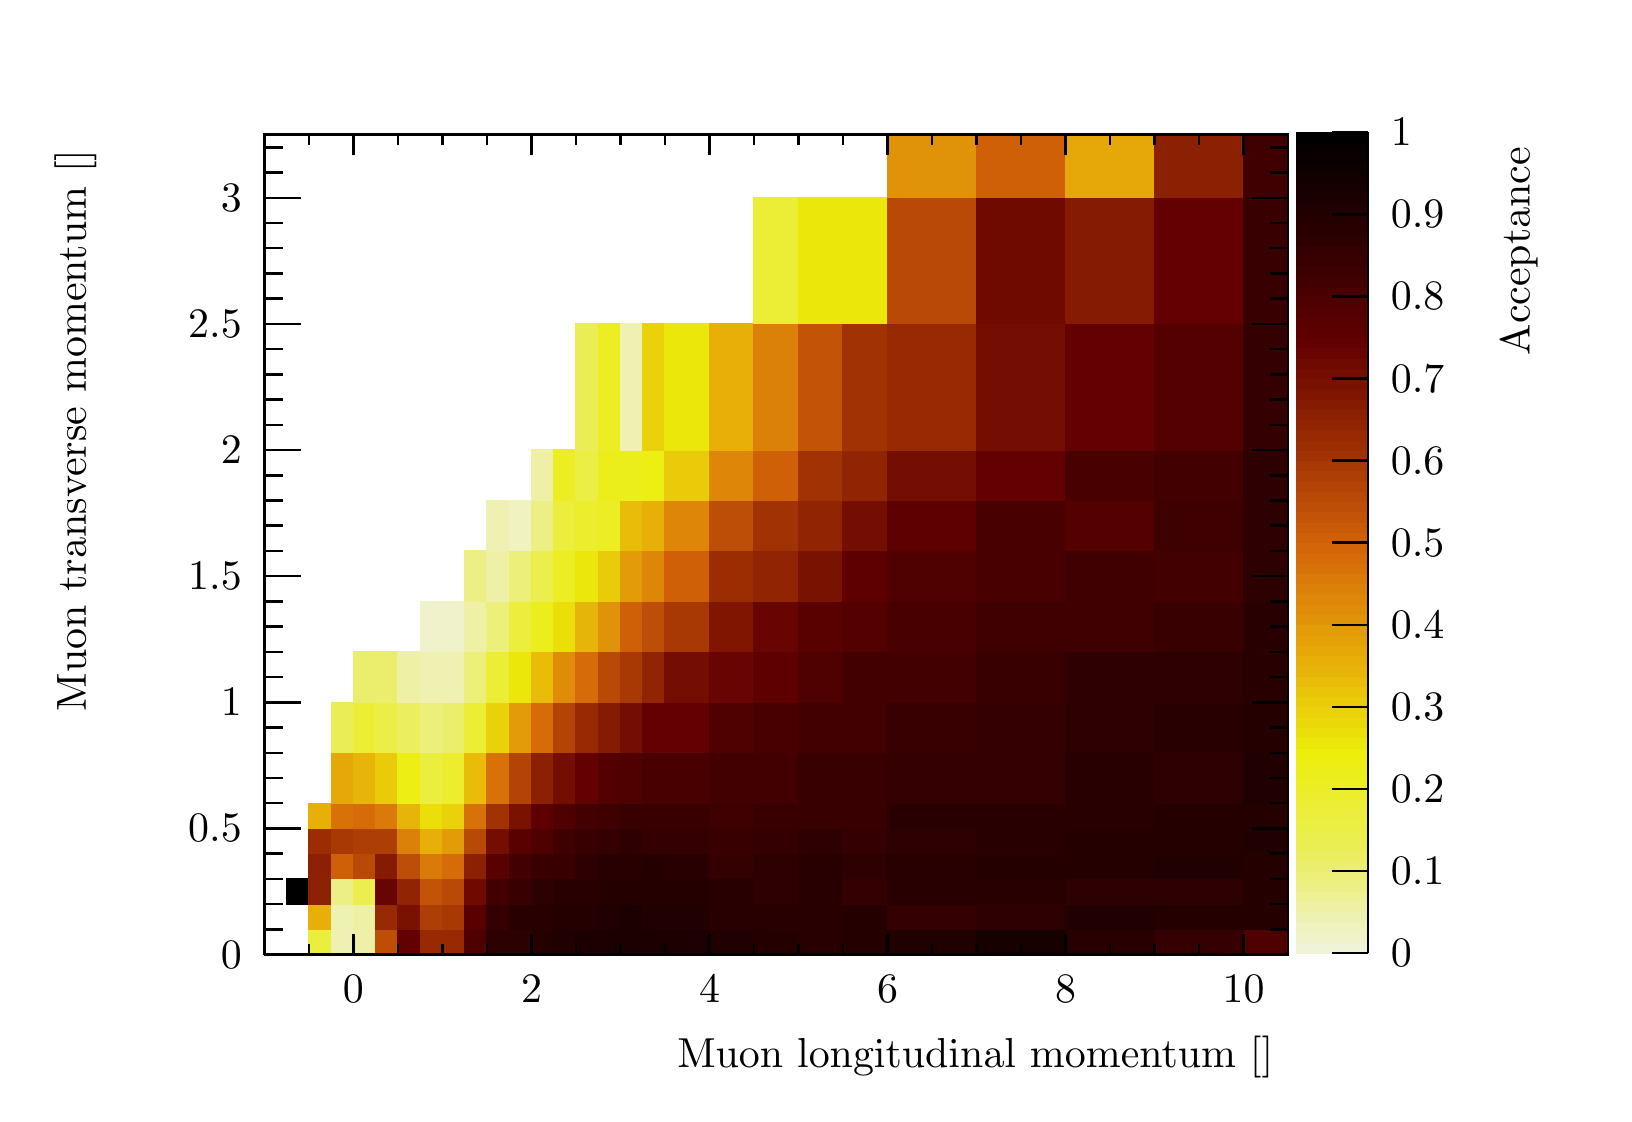
\begin{tikzpicture}
\pgfdeclareplotmark{cross} {
\pgfpathmoveto{\pgfpoint{-0.3\pgfplotmarksize}{\pgfplotmarksize}}
\pgfpathlineto{\pgfpoint{+0.3\pgfplotmarksize}{\pgfplotmarksize}}
\pgfpathlineto{\pgfpoint{+0.3\pgfplotmarksize}{0.3\pgfplotmarksize}}
\pgfpathlineto{\pgfpoint{+1\pgfplotmarksize}{0.3\pgfplotmarksize}}
\pgfpathlineto{\pgfpoint{+1\pgfplotmarksize}{-0.3\pgfplotmarksize}}
\pgfpathlineto{\pgfpoint{+0.3\pgfplotmarksize}{-0.3\pgfplotmarksize}}
\pgfpathlineto{\pgfpoint{+0.3\pgfplotmarksize}{-1.\pgfplotmarksize}}
\pgfpathlineto{\pgfpoint{-0.3\pgfplotmarksize}{-1.\pgfplotmarksize}}
\pgfpathlineto{\pgfpoint{-0.3\pgfplotmarksize}{-0.3\pgfplotmarksize}}
\pgfpathlineto{\pgfpoint{-1.\pgfplotmarksize}{-0.3\pgfplotmarksize}}
\pgfpathlineto{\pgfpoint{-1.\pgfplotmarksize}{0.3\pgfplotmarksize}}
\pgfpathlineto{\pgfpoint{-0.3\pgfplotmarksize}{0.3\pgfplotmarksize}}
\pgfpathclose
\pgfusepathqstroke
}
\pgfdeclareplotmark{cross*} {
\pgfpathmoveto{\pgfpoint{-0.3\pgfplotmarksize}{\pgfplotmarksize}}
\pgfpathlineto{\pgfpoint{+0.3\pgfplotmarksize}{\pgfplotmarksize}}
\pgfpathlineto{\pgfpoint{+0.3\pgfplotmarksize}{0.3\pgfplotmarksize}}
\pgfpathlineto{\pgfpoint{+1\pgfplotmarksize}{0.3\pgfplotmarksize}}
\pgfpathlineto{\pgfpoint{+1\pgfplotmarksize}{-0.3\pgfplotmarksize}}
\pgfpathlineto{\pgfpoint{+0.3\pgfplotmarksize}{-0.3\pgfplotmarksize}}
\pgfpathlineto{\pgfpoint{+0.3\pgfplotmarksize}{-1.\pgfplotmarksize}}
\pgfpathlineto{\pgfpoint{-0.3\pgfplotmarksize}{-1.\pgfplotmarksize}}
\pgfpathlineto{\pgfpoint{-0.3\pgfplotmarksize}{-0.3\pgfplotmarksize}}
\pgfpathlineto{\pgfpoint{-1.\pgfplotmarksize}{-0.3\pgfplotmarksize}}
\pgfpathlineto{\pgfpoint{-1.\pgfplotmarksize}{0.3\pgfplotmarksize}}
\pgfpathlineto{\pgfpoint{-0.3\pgfplotmarksize}{0.3\pgfplotmarksize}}
\pgfpathclose
\pgfusepathqfillstroke
}
\pgfdeclareplotmark{newstar} {
\pgfpathmoveto{\pgfqpoint{0pt}{\pgfplotmarksize}}
\pgfpathlineto{\pgfqpointpolar{44}{0.5\pgfplotmarksize}}
\pgfpathlineto{\pgfqpointpolar{18}{\pgfplotmarksize}}
\pgfpathlineto{\pgfqpointpolar{-20}{0.5\pgfplotmarksize}}
\pgfpathlineto{\pgfqpointpolar{-54}{\pgfplotmarksize}}
\pgfpathlineto{\pgfqpointpolar{-90}{0.5\pgfplotmarksize}}
\pgfpathlineto{\pgfqpointpolar{234}{\pgfplotmarksize}}
\pgfpathlineto{\pgfqpointpolar{198}{0.5\pgfplotmarksize}}
\pgfpathlineto{\pgfqpointpolar{162}{\pgfplotmarksize}}
\pgfpathlineto{\pgfqpointpolar{134}{0.5\pgfplotmarksize}}
\pgfpathclose
\pgfusepathqstroke
}
\pgfdeclareplotmark{newstar*} {
\pgfpathmoveto{\pgfqpoint{0pt}{\pgfplotmarksize}}
\pgfpathlineto{\pgfqpointpolar{44}{0.5\pgfplotmarksize}}
\pgfpathlineto{\pgfqpointpolar{18}{\pgfplotmarksize}}
\pgfpathlineto{\pgfqpointpolar{-20}{0.5\pgfplotmarksize}}
\pgfpathlineto{\pgfqpointpolar{-54}{\pgfplotmarksize}}
\pgfpathlineto{\pgfqpointpolar{-90}{0.5\pgfplotmarksize}}
\pgfpathlineto{\pgfqpointpolar{234}{\pgfplotmarksize}}
\pgfpathlineto{\pgfqpointpolar{198}{0.5\pgfplotmarksize}}
\pgfpathlineto{\pgfqpointpolar{162}{\pgfplotmarksize}}
\pgfpathlineto{\pgfqpointpolar{134}{0.5\pgfplotmarksize}}
\pgfpathclose
\pgfusepathqfillstroke
}
\definecolor{c}{rgb}{1,1,1};
\draw [color=c, fill=c] (0,0) rectangle (20,13.5227);
\draw [color=c, fill=c] (3,1.75795) rectangle (16,12.1705);
\definecolor{c}{rgb}{0,0,0};
\draw [c,line width=0.9] (3,1.75795) -- (3,12.1705) -- (16,12.1705) -- (16,1.75795) -- (3,1.75795);
\definecolor{c}{rgb}{1,1,1};
\draw [color=c, fill=c] (3,1.75795) rectangle (16,12.1705);
\definecolor{c}{rgb}{0,0,0};
\draw [c,line width=0.9] (3,1.75795) -- (3,12.1705) -- (16,12.1705) -- (16,1.75795) -- (3,1.75795);
\definecolor{c}{rgb}{0.922426,0.933333,0.238725};
\draw [color=c, fill=c] (3.56522,1.75795) rectangle (3.84783,2.07834);
\definecolor{c}{rgb}{0.936875,0.945351,0.697027};
\draw [color=c, fill=c] (3.84783,1.75795) rectangle (4.13043,2.07834);
\definecolor{c}{rgb}{0.933839,0.943453,0.645794};
\draw [color=c, fill=c] (4.13043,1.75795) rectangle (4.41304,2.07834);
\definecolor{c}{rgb}{0.742157,0.306863,0.0257353};
\draw [color=c, fill=c] (4.41304,1.75795) rectangle (4.69565,2.07834);
\definecolor{c}{rgb}{0.388235,0,0.00392157};
\draw [color=c, fill=c] (4.69565,1.75795) rectangle (4.97826,2.07834);
\definecolor{c}{rgb}{0.590809,0.159926,0.0110294};
\draw [color=c, fill=c] (4.97826,1.75795) rectangle (5.26087,2.07834);
\draw [color=c, fill=c] (5.26087,1.75795) rectangle (5.54348,2.07834);
\definecolor{c}{rgb}{0.308824,0,0.00392157};
\draw [color=c, fill=c] (5.54348,1.75795) rectangle (5.82609,2.07834);
\definecolor{c}{rgb}{0.176471,0,0.00392157};
\draw [color=c, fill=c] (5.82609,1.75795) rectangle (6.1087,2.07834);
\draw [color=c, fill=c] (6.1087,1.75795) rectangle (6.3913,2.07834);
\definecolor{c}{rgb}{0.143382,0,0.00318627};
\draw [color=c, fill=c] (6.3913,1.75795) rectangle (6.67391,2.07834);
\definecolor{c}{rgb}{0.126838,0,0.00281863};
\draw [color=c, fill=c] (6.67391,1.75795) rectangle (6.95652,2.07834);
\definecolor{c}{rgb}{0.110294,0,0.00245098};
\draw [color=c, fill=c] (6.95652,1.75795) rectangle (7.23913,2.07834);
\draw [color=c, fill=c] (7.23913,1.75795) rectangle (7.52174,2.07834);
\draw [color=c, fill=c] (7.52174,1.75795) rectangle (7.80435,2.07834);
\draw [color=c, fill=c] (7.80435,1.75795) rectangle (8.08696,2.07834);
\draw [color=c, fill=c] (8.08696,1.75795) rectangle (8.65217,2.07834);
\definecolor{c}{rgb}{0.126838,0,0.00281863};
\draw [color=c, fill=c] (8.65217,1.75795) rectangle (9.21739,2.07834);
\definecolor{c}{rgb}{0.143382,0,0.00318627};
\draw [color=c, fill=c] (9.21739,1.75795) rectangle (9.78261,2.07834);
\definecolor{c}{rgb}{0.159926,0,0.00355392};
\draw [color=c, fill=c] (9.78261,1.75795) rectangle (10.3478,2.07834);
\definecolor{c}{rgb}{0.143382,0,0.00318627};
\draw [color=c, fill=c] (10.3478,1.75795) rectangle (10.913,2.07834);
\definecolor{c}{rgb}{0.126838,0,0.00281863};
\draw [color=c, fill=c] (10.913,1.75795) rectangle (12.0435,2.07834);
\definecolor{c}{rgb}{0.0882353,0,0.00196078};
\draw [color=c, fill=c] (12.0435,1.75795) rectangle (13.1739,2.07834);
\definecolor{c}{rgb}{0.159926,0,0.00355392};
\draw [color=c, fill=c] (13.1739,1.75795) rectangle (14.3043,2.07834);
\definecolor{c}{rgb}{0.202941,0,0.00392157};
\draw [color=c, fill=c] (14.3043,1.75795) rectangle (15.4348,2.07834);
\definecolor{c}{rgb}{0.308824,0,0.00392157};
\draw [color=c, fill=c] (15.4348,1.75795) rectangle (16,2.07834);
\definecolor{c}{rgb}{0.904534,0.684559,0.0324755};
\draw [color=c, fill=c] (3.56522,2.07834) rectangle (3.84783,2.39872);
\definecolor{c}{rgb}{0.936875,0.945351,0.697027};
\draw [color=c, fill=c] (3.84783,2.07834) rectangle (4.13043,2.39872);
\definecolor{c}{rgb}{0.933839,0.943453,0.645794};
\draw [color=c, fill=c] (4.13043,2.07834) rectangle (4.41304,2.39872);
\definecolor{c}{rgb}{0.590809,0.159926,0.0110294};
\draw [color=c, fill=c] (4.41304,2.07834) rectangle (4.69565,2.39872);
\definecolor{c}{rgb}{0.479044,0.0716912,0.00710784};
\draw [color=c, fill=c] (4.69565,2.07834) rectangle (4.97826,2.39872);
\definecolor{c}{rgb}{0.680392,0.245098,0.0191176};
\draw [color=c, fill=c] (4.97826,2.07834) rectangle (5.26087,2.39872);
\definecolor{c}{rgb}{0.659804,0.22451,0.0169118};
\draw [color=c, fill=c] (5.26087,2.07834) rectangle (5.54348,2.39872);
\definecolor{c}{rgb}{0.348529,0,0.00392157};
\draw [color=c, fill=c] (5.54348,2.07834) rectangle (5.82609,2.39872);
\definecolor{c}{rgb}{0.202941,0,0.00392157};
\draw [color=c, fill=c] (5.82609,2.07834) rectangle (6.1087,2.39872);
\definecolor{c}{rgb}{0.159926,0,0.00355392};
\draw [color=c, fill=c] (6.1087,2.07834) rectangle (6.3913,2.39872);
\draw [color=c, fill=c] (6.3913,2.07834) rectangle (6.67391,2.39872);
\definecolor{c}{rgb}{0.143382,0,0.00318627};
\draw [color=c, fill=c] (6.67391,2.07834) rectangle (6.95652,2.39872);
\draw [color=c, fill=c] (6.95652,2.07834) rectangle (7.23913,2.39872);
\definecolor{c}{rgb}{0.126838,0,0.00281863};
\draw [color=c, fill=c] (7.23913,2.07834) rectangle (7.52174,2.39872);
\definecolor{c}{rgb}{0.110294,0,0.00245098};
\draw [color=c, fill=c] (7.52174,2.07834) rectangle (7.80435,2.39872);
\definecolor{c}{rgb}{0.126838,0,0.00281863};
\draw [color=c, fill=c] (7.80435,2.07834) rectangle (8.08696,2.39872);
\draw [color=c, fill=c] (8.08696,2.07834) rectangle (8.65217,2.39872);
\definecolor{c}{rgb}{0.159926,0,0.00355392};
\draw [color=c, fill=c] (8.65217,2.07834) rectangle (9.21739,2.39872);
\draw [color=c, fill=c] (9.21739,2.07834) rectangle (9.78261,2.39872);
\draw [color=c, fill=c] (9.78261,2.07834) rectangle (10.3478,2.39872);
\definecolor{c}{rgb}{0.143382,0,0.00318627};
\draw [color=c, fill=c] (10.3478,2.07834) rectangle (10.913,2.39872);
\definecolor{c}{rgb}{0.202941,0,0.00392157};
\draw [color=c, fill=c] (10.913,2.07834) rectangle (12.0435,2.39872);
\definecolor{c}{rgb}{0.176471,0,0.00392157};
\draw [color=c, fill=c] (12.0435,2.07834) rectangle (13.1739,2.39872);
\definecolor{c}{rgb}{0.126838,0,0.00281863};
\draw [color=c, fill=c] (13.1739,2.07834) rectangle (14.3043,2.39872);
\definecolor{c}{rgb}{0.143382,0,0.00318627};
\draw [color=c, fill=c] (14.3043,2.07834) rectangle (15.4348,2.39872);
\draw [color=c, fill=c] (15.4348,2.07834) rectangle (16,2.39872);
\definecolor{c}{rgb}{0.00551471,0,0.000122549};
\draw [color=c, fill=c] (3.28261,2.39872) rectangle (3.56522,2.71911);
\definecolor{c}{rgb}{0.548897,0.126838,0.00955882};
\draw [color=c, fill=c] (3.56522,2.39872) rectangle (3.84783,2.71911);
\definecolor{c}{rgb}{0.926755,0.939026,0.526249};
\draw [color=c, fill=c] (3.84783,2.39872) rectangle (4.13043,2.71911);
\definecolor{c}{rgb}{0.920221,0.933333,0.30049};
\draw [color=c, fill=c] (4.13043,2.39872) rectangle (4.41304,2.71911);
\definecolor{c}{rgb}{0.409191,0.0165441,0.00465686};
\draw [color=c, fill=c] (4.41304,2.39872) rectangle (4.69565,2.71911);
\definecolor{c}{rgb}{0.569853,0.143382,0.0102941};
\draw [color=c, fill=c] (4.69565,2.39872) rectangle (4.97826,2.71911);
\definecolor{c}{rgb}{0.762745,0.327451,0.0279412};
\draw [color=c, fill=c] (4.97826,2.39872) rectangle (5.26087,2.71911);
\definecolor{c}{rgb}{0.721569,0.286275,0.0235294};
\draw [color=c, fill=c] (5.26087,2.39872) rectangle (5.54348,2.71911);
\definecolor{c}{rgb}{0.437132,0.0386029,0.00563726};
\draw [color=c, fill=c] (5.54348,2.39872) rectangle (5.82609,2.71911);
\definecolor{c}{rgb}{0.2625,0,0.00392157};
\draw [color=c, fill=c] (5.82609,2.39872) rectangle (6.1087,2.71911);
\definecolor{c}{rgb}{0.222794,0,0.00392157};
\draw [color=c, fill=c] (6.1087,2.39872) rectangle (6.3913,2.71911);
\definecolor{c}{rgb}{0.176471,0,0.00392157};
\draw [color=c, fill=c] (6.3913,2.39872) rectangle (6.67391,2.71911);
\definecolor{c}{rgb}{0.159926,0,0.00355392};
\draw [color=c, fill=c] (6.67391,2.39872) rectangle (6.95652,2.71911);
\draw [color=c, fill=c] (6.95652,2.39872) rectangle (7.23913,2.71911);
\definecolor{c}{rgb}{0.143382,0,0.00318627};
\draw [color=c, fill=c] (7.23913,2.39872) rectangle (7.52174,2.71911);
\draw [color=c, fill=c] (7.52174,2.39872) rectangle (7.80435,2.71911);
\draw [color=c, fill=c] (7.80435,2.39872) rectangle (8.08696,2.71911);
\draw [color=c, fill=c] (8.08696,2.39872) rectangle (8.65217,2.71911);
\definecolor{c}{rgb}{0.159926,0,0.00355392};
\draw [color=c, fill=c] (8.65217,2.39872) rectangle (9.21739,2.71911);
\definecolor{c}{rgb}{0.176471,0,0.00392157};
\draw [color=c, fill=c] (9.21739,2.39872) rectangle (9.78261,2.71911);
\definecolor{c}{rgb}{0.159926,0,0.00355392};
\draw [color=c, fill=c] (9.78261,2.39872) rectangle (10.3478,2.71911);
\definecolor{c}{rgb}{0.202941,0,0.00392157};
\draw [color=c, fill=c] (10.3478,2.39872) rectangle (10.913,2.71911);
\definecolor{c}{rgb}{0.159926,0,0.00355392};
\draw [color=c, fill=c] (10.913,2.39872) rectangle (12.0435,2.71911);
\draw [color=c, fill=c] (12.0435,2.39872) rectangle (13.1739,2.71911);
\definecolor{c}{rgb}{0.176471,0,0.00392157};
\draw [color=c, fill=c] (13.1739,2.39872) rectangle (14.3043,2.71911);
\draw [color=c, fill=c] (14.3043,2.39872) rectangle (15.4348,2.71911);
\definecolor{c}{rgb}{0.143382,0,0.00318627};
\draw [color=c, fill=c] (15.4348,2.39872) rectangle (16,2.71911);
\definecolor{c}{rgb}{0.548897,0.126838,0.00955882};
\draw [color=c, fill=c] (3.56522,2.71911) rectangle (3.84783,3.03949);
\definecolor{c}{rgb}{0.810784,0.37549,0.0330882};
\draw [color=c, fill=c] (3.84783,2.71911) rectangle (4.13043,3.03949);
\definecolor{c}{rgb}{0.721569,0.286275,0.0235294};
\draw [color=c, fill=c] (4.13043,2.71911) rectangle (4.41304,3.03949);
\definecolor{c}{rgb}{0.520956,0.104779,0.00857843};
\draw [color=c, fill=c] (4.41304,2.71911) rectangle (4.69565,3.03949);
\definecolor{c}{rgb}{0.742157,0.306863,0.0257353};
\draw [color=c, fill=c] (4.69565,2.71911) rectangle (4.97826,3.03949);
\definecolor{c}{rgb}{0.853431,0.478186,0.0340686};
\draw [color=c, fill=c] (4.97826,2.71911) rectangle (5.26087,3.03949);
\definecolor{c}{rgb}{0.83799,0.420711,0.0349265};
\draw [color=c, fill=c] (5.26087,2.71911) rectangle (5.54348,3.03949);
\definecolor{c}{rgb}{0.548897,0.126838,0.00955882};
\draw [color=c, fill=c] (5.54348,2.71911) rectangle (5.82609,3.03949);
\definecolor{c}{rgb}{0.348529,0,0.00392157};
\draw [color=c, fill=c] (5.82609,2.71911) rectangle (6.1087,3.03949);
\definecolor{c}{rgb}{0.2625,0,0.00392157};
\draw [color=c, fill=c] (6.1087,2.71911) rectangle (6.3913,3.03949);
\definecolor{c}{rgb}{0.222794,0,0.00392157};
\draw [color=c, fill=c] (6.3913,2.71911) rectangle (6.67391,3.03949);
\draw [color=c, fill=c] (6.67391,2.71911) rectangle (6.95652,3.03949);
\definecolor{c}{rgb}{0.176471,0,0.00392157};
\draw [color=c, fill=c] (6.95652,2.71911) rectangle (7.23913,3.03949);
\definecolor{c}{rgb}{0.159926,0,0.00355392};
\draw [color=c, fill=c] (7.23913,2.71911) rectangle (7.52174,3.03949);
\draw [color=c, fill=c] (7.52174,2.71911) rectangle (7.80435,3.03949);
\definecolor{c}{rgb}{0.143382,0,0.00318627};
\draw [color=c, fill=c] (7.80435,2.71911) rectangle (8.08696,3.03949);
\definecolor{c}{rgb}{0.159926,0,0.00355392};
\draw [color=c, fill=c] (8.08696,2.71911) rectangle (8.65217,3.03949);
\definecolor{c}{rgb}{0.202941,0,0.00392157};
\draw [color=c, fill=c] (8.65217,2.71911) rectangle (9.21739,3.03949);
\definecolor{c}{rgb}{0.176471,0,0.00392157};
\draw [color=c, fill=c] (9.21739,2.71911) rectangle (9.78261,3.03949);
\definecolor{c}{rgb}{0.159926,0,0.00355392};
\draw [color=c, fill=c] (9.78261,2.71911) rectangle (10.3478,3.03949);
\definecolor{c}{rgb}{0.176471,0,0.00392157};
\draw [color=c, fill=c] (10.3478,2.71911) rectangle (10.913,3.03949);
\definecolor{c}{rgb}{0.159926,0,0.00355392};
\draw [color=c, fill=c] (10.913,2.71911) rectangle (12.0435,3.03949);
\definecolor{c}{rgb}{0.143382,0,0.00318627};
\draw [color=c, fill=c] (12.0435,2.71911) rectangle (13.1739,3.03949);
\draw [color=c, fill=c] (13.1739,2.71911) rectangle (14.3043,3.03949);
\definecolor{c}{rgb}{0.126838,0,0.00281863};
\draw [color=c, fill=c] (14.3043,2.71911) rectangle (15.4348,3.03949);
\definecolor{c}{rgb}{0.143382,0,0.00318627};
\draw [color=c, fill=c] (15.4348,2.71911) rectangle (16,3.03949);
\definecolor{c}{rgb}{0.611765,0.176471,0.0117647};
\draw [color=c, fill=c] (3.56522,3.03949) rectangle (3.84783,3.35988);
\definecolor{c}{rgb}{0.659804,0.22451,0.0169118};
\draw [color=c, fill=c] (3.84783,3.03949) rectangle (4.13043,3.35988);
\definecolor{c}{rgb}{0.680392,0.245098,0.0191176};
\draw [color=c, fill=c] (4.13043,3.03949) rectangle (4.41304,3.35988);
\draw [color=c, fill=c] (4.41304,3.03949) rectangle (4.69565,3.35988);
\definecolor{c}{rgb}{0.860049,0.502819,0.033701};
\draw [color=c, fill=c] (4.69565,3.03949) rectangle (4.97826,3.35988);
\definecolor{c}{rgb}{0.904534,0.684559,0.0324755};
\draw [color=c, fill=c] (4.97826,3.03949) rectangle (5.26087,3.35988);
\definecolor{c}{rgb}{0.888726,0.609559,0.0321078};
\draw [color=c, fill=c] (5.26087,3.03949) rectangle (5.54348,3.35988);
\definecolor{c}{rgb}{0.721569,0.286275,0.0235294};
\draw [color=c, fill=c] (5.54348,3.03949) rectangle (5.82609,3.35988);
\definecolor{c}{rgb}{0.458088,0.0551471,0.00637255};
\draw [color=c, fill=c] (5.82609,3.03949) rectangle (6.1087,3.35988);
\definecolor{c}{rgb}{0.348529,0,0.00392157};
\draw [color=c, fill=c] (6.1087,3.03949) rectangle (6.3913,3.35988);
\definecolor{c}{rgb}{0.308824,0,0.00392157};
\draw [color=c, fill=c] (6.3913,3.03949) rectangle (6.67391,3.35988);
\definecolor{c}{rgb}{0.242647,0,0.00392157};
\draw [color=c, fill=c] (6.67391,3.03949) rectangle (6.95652,3.35988);
\definecolor{c}{rgb}{0.222794,0,0.00392157};
\draw [color=c, fill=c] (6.95652,3.03949) rectangle (7.23913,3.35988);
\definecolor{c}{rgb}{0.202941,0,0.00392157};
\draw [color=c, fill=c] (7.23913,3.03949) rectangle (7.52174,3.35988);
\definecolor{c}{rgb}{0.176471,0,0.00392157};
\draw [color=c, fill=c] (7.52174,3.03949) rectangle (7.80435,3.35988);
\definecolor{c}{rgb}{0.202941,0,0.00392157};
\draw [color=c, fill=c] (7.80435,3.03949) rectangle (8.08696,3.35988);
\draw [color=c, fill=c] (8.08696,3.03949) rectangle (8.65217,3.35988);
\definecolor{c}{rgb}{0.222794,0,0.00392157};
\draw [color=c, fill=c] (8.65217,3.03949) rectangle (9.21739,3.35988);
\definecolor{c}{rgb}{0.202941,0,0.00392157};
\draw [color=c, fill=c] (9.21739,3.03949) rectangle (9.78261,3.35988);
\definecolor{c}{rgb}{0.176471,0,0.00392157};
\draw [color=c, fill=c] (9.78261,3.03949) rectangle (10.3478,3.35988);
\definecolor{c}{rgb}{0.202941,0,0.00392157};
\draw [color=c, fill=c] (10.3478,3.03949) rectangle (10.913,3.35988);
\definecolor{c}{rgb}{0.176471,0,0.00392157};
\draw [color=c, fill=c] (10.913,3.03949) rectangle (12.0435,3.35988);
\definecolor{c}{rgb}{0.159926,0,0.00355392};
\draw [color=c, fill=c] (12.0435,3.03949) rectangle (13.1739,3.35988);
\definecolor{c}{rgb}{0.143382,0,0.00318627};
\draw [color=c, fill=c] (13.1739,3.03949) rectangle (14.3043,3.35988);
\draw [color=c, fill=c] (14.3043,3.03949) rectangle (15.4348,3.35988);
\definecolor{c}{rgb}{0.126838,0,0.00281863};
\draw [color=c, fill=c] (15.4348,3.03949) rectangle (16,3.35988);
\definecolor{c}{rgb}{0.904534,0.684559,0.0324755};
\draw [color=c, fill=c] (3.56522,3.35988) rectangle (3.84783,3.68026);
\definecolor{c}{rgb}{0.844608,0.445343,0.0345588};
\draw [color=c, fill=c] (3.84783,3.35988) rectangle (4.13043,3.68026);
\definecolor{c}{rgb}{0.83799,0.420711,0.0349265};
\draw [color=c, fill=c] (4.13043,3.35988) rectangle (4.41304,3.68026);
\definecolor{c}{rgb}{0.853431,0.478186,0.0340686};
\draw [color=c, fill=c] (4.41304,3.35988) rectangle (4.69565,3.68026);
\definecolor{c}{rgb}{0.907108,0.710294,0.0335784};
\draw [color=c, fill=c] (4.69565,3.35988) rectangle (4.97826,3.68026);
\definecolor{c}{rgb}{0.923407,0.873284,0.0405637};
\draw [color=c, fill=c] (4.97826,3.35988) rectangle (5.26087,3.68026);
\definecolor{c}{rgb}{0.91826,0.821814,0.0383578};
\draw [color=c, fill=c] (5.26087,3.35988) rectangle (5.54348,3.68026);
\definecolor{c}{rgb}{0.844608,0.445343,0.0345588};
\draw [color=c, fill=c] (5.54348,3.35988) rectangle (5.82609,3.68026);
\definecolor{c}{rgb}{0.632353,0.197059,0.0139706};
\draw [color=c, fill=c] (5.82609,3.35988) rectangle (6.1087,3.68026);
\definecolor{c}{rgb}{0.479044,0.0716912,0.00710784};
\draw [color=c, fill=c] (6.1087,3.35988) rectangle (6.3913,3.68026);
\definecolor{c}{rgb}{0.368382,0,0.00392157};
\draw [color=c, fill=c] (6.3913,3.35988) rectangle (6.67391,3.68026);
\definecolor{c}{rgb}{0.308824,0,0.00392157};
\draw [color=c, fill=c] (6.67391,3.35988) rectangle (6.95652,3.68026);
\definecolor{c}{rgb}{0.2625,0,0.00392157};
\draw [color=c, fill=c] (6.95652,3.35988) rectangle (7.23913,3.68026);
\definecolor{c}{rgb}{0.242647,0,0.00392157};
\draw [color=c, fill=c] (7.23913,3.35988) rectangle (7.52174,3.68026);
\definecolor{c}{rgb}{0.222794,0,0.00392157};
\draw [color=c, fill=c] (7.52174,3.35988) rectangle (7.80435,3.68026);
\draw [color=c, fill=c] (7.80435,3.35988) rectangle (8.08696,3.68026);
\draw [color=c, fill=c] (8.08696,3.35988) rectangle (8.65217,3.68026);
\definecolor{c}{rgb}{0.242647,0,0.00392157};
\draw [color=c, fill=c] (8.65217,3.35988) rectangle (9.21739,3.68026);
\definecolor{c}{rgb}{0.222794,0,0.00392157};
\draw [color=c, fill=c] (9.21739,3.35988) rectangle (9.78261,3.68026);
\draw [color=c, fill=c] (9.78261,3.35988) rectangle (10.3478,3.68026);
\draw [color=c, fill=c] (10.3478,3.35988) rectangle (10.913,3.68026);
\definecolor{c}{rgb}{0.159926,0,0.00355392};
\draw [color=c, fill=c] (10.913,3.35988) rectangle (12.0435,3.68026);
\draw [color=c, fill=c] (12.0435,3.35988) rectangle (13.1739,3.68026);
\draw [color=c, fill=c] (13.1739,3.35988) rectangle (14.3043,3.68026);
\definecolor{c}{rgb}{0.143382,0,0.00318627};
\draw [color=c, fill=c] (14.3043,3.35988) rectangle (15.4348,3.68026);
\draw [color=c, fill=c] (15.4348,3.35988) rectangle (16,3.68026);
\definecolor{c}{rgb}{0.901961,0.658824,0.0313726};
\draw [color=c, fill=c] (3.84783,3.68026) rectangle (4.13043,4.32103);
\definecolor{c}{rgb}{0.907108,0.710294,0.0335784};
\draw [color=c, fill=c] (4.13043,3.68026) rectangle (4.41304,4.32103);
\definecolor{c}{rgb}{0.915686,0.796078,0.0372549};
\draw [color=c, fill=c] (4.41304,3.68026) rectangle (4.69565,4.32103);
\definecolor{c}{rgb}{0.928309,0.933333,0.0740196};
\draw [color=c, fill=c] (4.69565,3.68026) rectangle (4.97826,4.32103);
\definecolor{c}{rgb}{0.922426,0.933333,0.238725};
\draw [color=c, fill=c] (4.97826,3.68026) rectangle (5.26087,4.32103);
\definecolor{c}{rgb}{0.924632,0.933333,0.176961};
\draw [color=c, fill=c] (5.26087,3.68026) rectangle (5.54348,4.32103);
\definecolor{c}{rgb}{0.909681,0.736029,0.0346814};
\draw [color=c, fill=c] (5.54348,3.68026) rectangle (5.82609,4.32103);
\definecolor{c}{rgb}{0.844608,0.445343,0.0345588};
\draw [color=c, fill=c] (5.82609,3.68026) rectangle (6.1087,4.32103);
\definecolor{c}{rgb}{0.70098,0.265686,0.0213235};
\draw [color=c, fill=c] (6.1087,3.68026) rectangle (6.3913,4.32103);
\definecolor{c}{rgb}{0.548897,0.126838,0.00955882};
\draw [color=c, fill=c] (6.3913,3.68026) rectangle (6.67391,4.32103);
\definecolor{c}{rgb}{0.458088,0.0551471,0.00637255};
\draw [color=c, fill=c] (6.67391,3.68026) rectangle (6.95652,4.32103);
\definecolor{c}{rgb}{0.388235,0,0.00392157};
\draw [color=c, fill=c] (6.95652,3.68026) rectangle (7.23913,4.32103);
\definecolor{c}{rgb}{0.328676,0,0.00392157};
\draw [color=c, fill=c] (7.23913,3.68026) rectangle (7.52174,4.32103);
\definecolor{c}{rgb}{0.308824,0,0.00392157};
\draw [color=c, fill=c] (7.52174,3.68026) rectangle (7.80435,4.32103);
\definecolor{c}{rgb}{0.282353,0,0.00392157};
\draw [color=c, fill=c] (7.80435,3.68026) rectangle (8.08696,4.32103);
\draw [color=c, fill=c] (8.08696,3.68026) rectangle (8.65217,4.32103);
\definecolor{c}{rgb}{0.2625,0,0.00392157};
\draw [color=c, fill=c] (8.65217,3.68026) rectangle (9.21739,4.32103);
\draw [color=c, fill=c] (9.21739,3.68026) rectangle (9.78261,4.32103);
\definecolor{c}{rgb}{0.222794,0,0.00392157};
\draw [color=c, fill=c] (9.78261,3.68026) rectangle (10.3478,4.32103);
\draw [color=c, fill=c] (10.3478,3.68026) rectangle (10.913,4.32103);
\definecolor{c}{rgb}{0.202941,0,0.00392157};
\draw [color=c, fill=c] (10.913,3.68026) rectangle (12.0435,4.32103);
\draw [color=c, fill=c] (12.0435,3.68026) rectangle (13.1739,4.32103);
\definecolor{c}{rgb}{0.159926,0,0.00355392};
\draw [color=c, fill=c] (13.1739,3.68026) rectangle (14.3043,4.32103);
\definecolor{c}{rgb}{0.176471,0,0.00392157};
\draw [color=c, fill=c] (14.3043,3.68026) rectangle (15.4348,4.32103);
\definecolor{c}{rgb}{0.126838,0,0.00281863};
\draw [color=c, fill=c] (15.4348,3.68026) rectangle (16,4.32103);
\definecolor{c}{rgb}{0.919118,0.933333,0.331373};
\draw [color=c, fill=c] (3.84783,4.32103) rectangle (4.13043,4.9618);
\definecolor{c}{rgb}{0.923529,0.933333,0.207843};
\draw [color=c, fill=c] (4.13043,4.32103) rectangle (4.41304,4.9618);
\definecolor{c}{rgb}{0.921324,0.933333,0.269608};
\draw [color=c, fill=c] (4.41304,4.32103) rectangle (4.69565,4.9618);
\definecolor{c}{rgb}{0.917647,0.933333,0.372549};
\draw [color=c, fill=c] (4.69565,4.32103) rectangle (4.97826,4.9618);
\definecolor{c}{rgb}{0.923719,0.937128,0.475016};
\draw [color=c, fill=c] (4.97826,4.32103) rectangle (5.26087,4.9618);
\definecolor{c}{rgb}{0.920683,0.935231,0.423782};
\draw [color=c, fill=c] (5.26087,4.32103) rectangle (5.54348,4.9618);
\definecolor{c}{rgb}{0.923529,0.933333,0.207843};
\draw [color=c, fill=c] (5.54348,4.32103) rectangle (5.82609,4.9618);
\definecolor{c}{rgb}{0.91826,0.821814,0.0383578};
\draw [color=c, fill=c] (5.82609,4.32103) rectangle (6.1087,4.9618);
\definecolor{c}{rgb}{0.888726,0.609559,0.0321078};
\draw [color=c, fill=c] (6.1087,4.32103) rectangle (6.3913,4.9618);
\definecolor{c}{rgb}{0.83799,0.420711,0.0349265};
\draw [color=c, fill=c] (6.3913,4.32103) rectangle (6.67391,4.9618);
\definecolor{c}{rgb}{0.70098,0.265686,0.0213235};
\draw [color=c, fill=c] (6.67391,4.32103) rectangle (6.95652,4.9618);
\definecolor{c}{rgb}{0.590809,0.159926,0.0110294};
\draw [color=c, fill=c] (6.95652,4.32103) rectangle (7.23913,4.9618);
\definecolor{c}{rgb}{0.520956,0.104779,0.00857843};
\draw [color=c, fill=c] (7.23913,4.32103) rectangle (7.52174,4.9618);
\definecolor{c}{rgb}{0.458088,0.0551471,0.00637255};
\draw [color=c, fill=c] (7.52174,4.32103) rectangle (7.80435,4.9618);
\definecolor{c}{rgb}{0.388235,0,0.00392157};
\draw [color=c, fill=c] (7.80435,4.32103) rectangle (8.08696,4.9618);
\draw [color=c, fill=c] (8.08696,4.32103) rectangle (8.65217,4.9618);
\definecolor{c}{rgb}{0.308824,0,0.00392157};
\draw [color=c, fill=c] (8.65217,4.32103) rectangle (9.21739,4.9618);
\definecolor{c}{rgb}{0.282353,0,0.00392157};
\draw [color=c, fill=c] (9.21739,4.32103) rectangle (9.78261,4.9618);
\definecolor{c}{rgb}{0.2625,0,0.00392157};
\draw [color=c, fill=c] (9.78261,4.32103) rectangle (10.3478,4.9618);
\draw [color=c, fill=c] (10.3478,4.32103) rectangle (10.913,4.9618);
\definecolor{c}{rgb}{0.222794,0,0.00392157};
\draw [color=c, fill=c] (10.913,4.32103) rectangle (12.0435,4.9618);
\definecolor{c}{rgb}{0.202941,0,0.00392157};
\draw [color=c, fill=c] (12.0435,4.32103) rectangle (13.1739,4.9618);
\definecolor{c}{rgb}{0.176471,0,0.00392157};
\draw [color=c, fill=c] (13.1739,4.32103) rectangle (14.3043,4.9618);
\definecolor{c}{rgb}{0.159926,0,0.00355392};
\draw [color=c, fill=c] (14.3043,4.32103) rectangle (15.4348,4.9618);
\definecolor{c}{rgb}{0.143382,0,0.00318627};
\draw [color=c, fill=c] (15.4348,4.32103) rectangle (16,4.9618);
\definecolor{c}{rgb}{0.920683,0.935231,0.423782};
\draw [color=c, fill=c] (4.13043,4.9618) rectangle (4.41304,5.60257);
\draw [color=c, fill=c] (4.41304,4.9618) rectangle (4.69565,5.60257);
\definecolor{c}{rgb}{0.933839,0.943453,0.645794};
\draw [color=c, fill=c] (4.69565,4.9618) rectangle (4.97826,5.60257);
\definecolor{c}{rgb}{0.936875,0.945351,0.697027};
\draw [color=c, fill=c] (4.97826,4.9618) rectangle (5.26087,5.60257);
\draw [color=c, fill=c] (5.26087,4.9618) rectangle (5.54348,5.60257);
\definecolor{c}{rgb}{0.923719,0.937128,0.475016};
\draw [color=c, fill=c] (5.54348,4.9618) rectangle (5.82609,5.60257);
\definecolor{c}{rgb}{0.923529,0.933333,0.207843};
\draw [color=c, fill=c] (5.82609,4.9618) rectangle (6.1087,5.60257);
\definecolor{c}{rgb}{0.926838,0.907598,0.0420343};
\draw [color=c, fill=c] (6.1087,4.9618) rectangle (6.3913,5.60257);
\definecolor{c}{rgb}{0.909681,0.736029,0.0346814};
\draw [color=c, fill=c] (6.3913,4.9618) rectangle (6.67391,5.60257);
\definecolor{c}{rgb}{0.873284,0.552083,0.0329657};
\draw [color=c, fill=c] (6.67391,4.9618) rectangle (6.95652,5.60257);
\definecolor{c}{rgb}{0.83799,0.420711,0.0349265};
\draw [color=c, fill=c] (6.95652,4.9618) rectangle (7.23913,5.60257);
\definecolor{c}{rgb}{0.721569,0.286275,0.0235294};
\draw [color=c, fill=c] (7.23913,4.9618) rectangle (7.52174,5.60257);
\definecolor{c}{rgb}{0.659804,0.22451,0.0169118};
\draw [color=c, fill=c] (7.52174,4.9618) rectangle (7.80435,5.60257);
\definecolor{c}{rgb}{0.569853,0.143382,0.0102941};
\draw [color=c, fill=c] (7.80435,4.9618) rectangle (8.08696,5.60257);
\definecolor{c}{rgb}{0.458088,0.0551471,0.00637255};
\draw [color=c, fill=c] (8.08696,4.9618) rectangle (8.65217,5.60257);
\definecolor{c}{rgb}{0.409191,0.0165441,0.00465686};
\draw [color=c, fill=c] (8.65217,4.9618) rectangle (9.21739,5.60257);
\definecolor{c}{rgb}{0.368382,0,0.00392157};
\draw [color=c, fill=c] (9.21739,4.9618) rectangle (9.78261,5.60257);
\definecolor{c}{rgb}{0.308824,0,0.00392157};
\draw [color=c, fill=c] (9.78261,4.9618) rectangle (10.3478,5.60257);
\definecolor{c}{rgb}{0.2625,0,0.00392157};
\draw [color=c, fill=c] (10.3478,4.9618) rectangle (10.913,5.60257);
\draw [color=c, fill=c] (10.913,4.9618) rectangle (12.0435,5.60257);
\definecolor{c}{rgb}{0.222794,0,0.00392157};
\draw [color=c, fill=c] (12.0435,4.9618) rectangle (13.1739,5.60257);
\definecolor{c}{rgb}{0.176471,0,0.00392157};
\draw [color=c, fill=c] (13.1739,4.9618) rectangle (14.3043,5.60257);
\draw [color=c, fill=c] (14.3043,4.9618) rectangle (15.4348,5.60257);
\definecolor{c}{rgb}{0.159926,0,0.00355392};
\draw [color=c, fill=c] (15.4348,4.9618) rectangle (16,5.60257);
\definecolor{c}{rgb}{0.942948,0.949146,0.799494};
\draw [color=c, fill=c] (4.97826,5.60257) rectangle (5.26087,6.24334);
\draw [color=c, fill=c] (5.26087,5.60257) rectangle (5.54348,6.24334);
\definecolor{c}{rgb}{0.933839,0.943453,0.645794};
\draw [color=c, fill=c] (5.54348,5.60257) rectangle (5.82609,6.24334);
\definecolor{c}{rgb}{0.923719,0.937128,0.475016};
\draw [color=c, fill=c] (5.82609,5.60257) rectangle (6.1087,6.24334);
\definecolor{c}{rgb}{0.922426,0.933333,0.238725};
\draw [color=c, fill=c] (6.1087,5.60257) rectangle (6.3913,6.24334);
\definecolor{c}{rgb}{0.927206,0.933333,0.104902};
\draw [color=c, fill=c] (6.3913,5.60257) rectangle (6.67391,6.24334);
\definecolor{c}{rgb}{0.923407,0.873284,0.0405637};
\draw [color=c, fill=c] (6.67391,5.60257) rectangle (6.95652,6.24334);
\definecolor{c}{rgb}{0.907108,0.710294,0.0335784};
\draw [color=c, fill=c] (6.95652,5.60257) rectangle (7.23913,6.24334);
\definecolor{c}{rgb}{0.879902,0.576716,0.032598};
\draw [color=c, fill=c] (7.23913,5.60257) rectangle (7.52174,6.24334);
\definecolor{c}{rgb}{0.810784,0.37549,0.0330882};
\draw [color=c, fill=c] (7.52174,5.60257) rectangle (7.80435,6.24334);
\definecolor{c}{rgb}{0.742157,0.306863,0.0257353};
\draw [color=c, fill=c] (7.80435,5.60257) rectangle (8.08696,6.24334);
\definecolor{c}{rgb}{0.659804,0.22451,0.0169118};
\draw [color=c, fill=c] (8.08696,5.60257) rectangle (8.65217,6.24334);
\definecolor{c}{rgb}{0.5,0.0882353,0.00784314};
\draw [color=c, fill=c] (8.65217,5.60257) rectangle (9.21739,6.24334);
\definecolor{c}{rgb}{0.409191,0.0165441,0.00465686};
\draw [color=c, fill=c] (9.21739,5.60257) rectangle (9.78261,6.24334);
\definecolor{c}{rgb}{0.348529,0,0.00392157};
\draw [color=c, fill=c] (9.78261,5.60257) rectangle (10.3478,6.24334);
\definecolor{c}{rgb}{0.328676,0,0.00392157};
\draw [color=c, fill=c] (10.3478,5.60257) rectangle (10.913,6.24334);
\definecolor{c}{rgb}{0.282353,0,0.00392157};
\draw [color=c, fill=c] (10.913,5.60257) rectangle (12.0435,6.24334);
\definecolor{c}{rgb}{0.242647,0,0.00392157};
\draw [color=c, fill=c] (12.0435,5.60257) rectangle (13.1739,6.24334);
\draw [color=c, fill=c] (13.1739,5.60257) rectangle (14.3043,6.24334);
\definecolor{c}{rgb}{0.222794,0,0.00392157};
\draw [color=c, fill=c] (14.3043,5.60257) rectangle (15.4348,6.24334);
\definecolor{c}{rgb}{0.159926,0,0.00355392};
\draw [color=c, fill=c] (15.4348,5.60257) rectangle (16,6.24334);
\definecolor{c}{rgb}{0.926755,0.939026,0.526249};
\draw [color=c, fill=c] (5.54348,6.24334) rectangle (5.82609,6.88411);
\definecolor{c}{rgb}{0.933839,0.943453,0.645794};
\draw [color=c, fill=c] (5.82609,6.24334) rectangle (6.1087,6.88411);
\definecolor{c}{rgb}{0.923719,0.937128,0.475016};
\draw [color=c, fill=c] (6.1087,6.24334) rectangle (6.3913,6.88411);
\definecolor{c}{rgb}{0.920221,0.933333,0.30049};
\draw [color=c, fill=c] (6.3913,6.24334) rectangle (6.67391,6.88411);
\definecolor{c}{rgb}{0.926103,0.933333,0.135784};
\draw [color=c, fill=c] (6.67391,6.24334) rectangle (6.95652,6.88411);
\definecolor{c}{rgb}{0.926838,0.907598,0.0420343};
\draw [color=c, fill=c] (6.95652,6.24334) rectangle (7.23913,6.88411);
\definecolor{c}{rgb}{0.915686,0.796078,0.0372549};
\draw [color=c, fill=c] (7.23913,6.24334) rectangle (7.52174,6.88411);
\definecolor{c}{rgb}{0.888726,0.609559,0.0321078};
\draw [color=c, fill=c] (7.52174,6.24334) rectangle (7.80435,6.88411);
\definecolor{c}{rgb}{0.866667,0.527451,0.0333333};
\draw [color=c, fill=c] (7.80435,6.24334) rectangle (8.08696,6.88411);
\definecolor{c}{rgb}{0.810784,0.37549,0.0330882};
\draw [color=c, fill=c] (8.08696,6.24334) rectangle (8.65217,6.88411);
\definecolor{c}{rgb}{0.611765,0.176471,0.0117647};
\draw [color=c, fill=c] (8.65217,6.24334) rectangle (9.21739,6.88411);
\definecolor{c}{rgb}{0.569853,0.143382,0.0102941};
\draw [color=c, fill=c] (9.21739,6.24334) rectangle (9.78261,6.88411);
\definecolor{c}{rgb}{0.479044,0.0716912,0.00710784};
\draw [color=c, fill=c] (9.78261,6.24334) rectangle (10.3478,6.88411);
\definecolor{c}{rgb}{0.368382,0,0.00392157};
\draw [color=c, fill=c] (10.3478,6.24334) rectangle (10.913,6.88411);
\definecolor{c}{rgb}{0.308824,0,0.00392157};
\draw [color=c, fill=c] (10.913,6.24334) rectangle (12.0435,6.88411);
\definecolor{c}{rgb}{0.282353,0,0.00392157};
\draw [color=c, fill=c] (12.0435,6.24334) rectangle (13.1739,6.88411);
\definecolor{c}{rgb}{0.242647,0,0.00392157};
\draw [color=c, fill=c] (13.1739,6.24334) rectangle (14.3043,6.88411);
\definecolor{c}{rgb}{0.2625,0,0.00392157};
\draw [color=c, fill=c] (14.3043,6.24334) rectangle (15.4348,6.88411);
\definecolor{c}{rgb}{0.176471,0,0.00392157};
\draw [color=c, fill=c] (15.4348,6.24334) rectangle (16,6.88411);
\definecolor{c}{rgb}{0.936875,0.945351,0.697027};
\draw [color=c, fill=c] (5.82609,6.88411) rectangle (6.1087,7.52488);
\definecolor{c}{rgb}{0.939911,0.947249,0.748261};
\draw [color=c, fill=c] (6.1087,6.88411) rectangle (6.3913,7.52488);
\definecolor{c}{rgb}{0.926755,0.939026,0.526249};
\draw [color=c, fill=c] (6.3913,6.88411) rectangle (6.67391,7.52488);
\definecolor{c}{rgb}{0.922426,0.933333,0.238725};
\draw [color=c, fill=c] (6.67391,6.88411) rectangle (6.95652,7.52488);
\definecolor{c}{rgb}{0.924632,0.933333,0.176961};
\draw [color=c, fill=c] (6.95652,6.88411) rectangle (7.23913,7.52488);
\definecolor{c}{rgb}{0.926103,0.933333,0.135784};
\draw [color=c, fill=c] (7.23913,6.88411) rectangle (7.52174,7.52488);
\definecolor{c}{rgb}{0.909681,0.736029,0.0346814};
\draw [color=c, fill=c] (7.52174,6.88411) rectangle (7.80435,7.52488);
\definecolor{c}{rgb}{0.904534,0.684559,0.0324755};
\draw [color=c, fill=c] (7.80435,6.88411) rectangle (8.08696,7.52488);
\definecolor{c}{rgb}{0.866667,0.527451,0.0333333};
\draw [color=c, fill=c] (8.08696,6.88411) rectangle (8.65217,7.52488);
\definecolor{c}{rgb}{0.742157,0.306863,0.0257353};
\draw [color=c, fill=c] (8.65217,6.88411) rectangle (9.21739,7.52488);
\definecolor{c}{rgb}{0.632353,0.197059,0.0139706};
\draw [color=c, fill=c] (9.21739,6.88411) rectangle (9.78261,7.52488);
\definecolor{c}{rgb}{0.569853,0.143382,0.0102941};
\draw [color=c, fill=c] (9.78261,6.88411) rectangle (10.3478,7.52488);
\definecolor{c}{rgb}{0.458088,0.0551471,0.00637255};
\draw [color=c, fill=c] (10.3478,6.88411) rectangle (10.913,7.52488);
\definecolor{c}{rgb}{0.368382,0,0.00392157};
\draw [color=c, fill=c] (10.913,6.88411) rectangle (12.0435,7.52488);
\definecolor{c}{rgb}{0.282353,0,0.00392157};
\draw [color=c, fill=c] (12.0435,6.88411) rectangle (13.1739,7.52488);
\definecolor{c}{rgb}{0.328676,0,0.00392157};
\draw [color=c, fill=c] (13.1739,6.88411) rectangle (14.3043,7.52488);
\definecolor{c}{rgb}{0.242647,0,0.00392157};
\draw [color=c, fill=c] (14.3043,6.88411) rectangle (15.4348,7.52488);
\definecolor{c}{rgb}{0.176471,0,0.00392157};
\draw [color=c, fill=c] (15.4348,6.88411) rectangle (16,7.52488);
\definecolor{c}{rgb}{0.933839,0.943453,0.645794};
\draw [color=c, fill=c] (6.3913,7.52488) rectangle (6.67391,8.16565);
\definecolor{c}{rgb}{0.926103,0.933333,0.135784};
\draw [color=c, fill=c] (6.67391,7.52488) rectangle (6.95652,8.16565);
\definecolor{c}{rgb}{0.921324,0.933333,0.269608};
\draw [color=c, fill=c] (6.95652,7.52488) rectangle (7.23913,8.16565);
\definecolor{c}{rgb}{0.927206,0.933333,0.104902};
\draw [color=c, fill=c] (7.23913,7.52488) rectangle (7.52174,8.16565);
\draw [color=c, fill=c] (7.52174,7.52488) rectangle (7.80435,8.16565);
\definecolor{c}{rgb}{0.928309,0.933333,0.0740196};
\draw [color=c, fill=c] (7.80435,7.52488) rectangle (8.08696,8.16565);
\definecolor{c}{rgb}{0.915686,0.796078,0.0372549};
\draw [color=c, fill=c] (8.08696,7.52488) rectangle (8.65217,8.16565);
\definecolor{c}{rgb}{0.866667,0.527451,0.0333333};
\draw [color=c, fill=c] (8.65217,7.52488) rectangle (9.21739,8.16565);
\definecolor{c}{rgb}{0.810784,0.37549,0.0330882};
\draw [color=c, fill=c] (9.21739,7.52488) rectangle (9.78261,8.16565);
\definecolor{c}{rgb}{0.632353,0.197059,0.0139706};
\draw [color=c, fill=c] (9.78261,7.52488) rectangle (10.3478,8.16565);
\definecolor{c}{rgb}{0.569853,0.143382,0.0102941};
\draw [color=c, fill=c] (10.3478,7.52488) rectangle (10.913,8.16565);
\definecolor{c}{rgb}{0.458088,0.0551471,0.00637255};
\draw [color=c, fill=c] (10.913,7.52488) rectangle (12.0435,8.16565);
\definecolor{c}{rgb}{0.388235,0,0.00392157};
\draw [color=c, fill=c] (12.0435,7.52488) rectangle (13.1739,8.16565);
\definecolor{c}{rgb}{0.282353,0,0.00392157};
\draw [color=c, fill=c] (13.1739,7.52488) rectangle (14.3043,8.16565);
\definecolor{c}{rgb}{0.2625,0,0.00392157};
\draw [color=c, fill=c] (14.3043,7.52488) rectangle (15.4348,8.16565);
\definecolor{c}{rgb}{0.176471,0,0.00392157};
\draw [color=c, fill=c] (15.4348,7.52488) rectangle (16,8.16565);
\definecolor{c}{rgb}{0.919118,0.933333,0.331373};
\draw [color=c, fill=c] (6.95652,8.16565) rectangle (7.23913,9.76757);
\definecolor{c}{rgb}{0.926103,0.933333,0.135784};
\draw [color=c, fill=c] (7.23913,8.16565) rectangle (7.52174,9.76757);
\definecolor{c}{rgb}{0.936875,0.945351,0.697027};
\draw [color=c, fill=c] (7.52174,8.16565) rectangle (7.80435,9.76757);
\definecolor{c}{rgb}{0.91826,0.821814,0.0383578};
\draw [color=c, fill=c] (7.80435,8.16565) rectangle (8.08696,9.76757);
\definecolor{c}{rgb}{0.926838,0.907598,0.0420343};
\draw [color=c, fill=c] (8.08696,8.16565) rectangle (8.65217,9.76757);
\definecolor{c}{rgb}{0.904534,0.684559,0.0324755};
\draw [color=c, fill=c] (8.65217,8.16565) rectangle (9.21739,9.76757);
\definecolor{c}{rgb}{0.860049,0.502819,0.033701};
\draw [color=c, fill=c] (9.21739,8.16565) rectangle (9.78261,9.76757);
\definecolor{c}{rgb}{0.762745,0.327451,0.0279412};
\draw [color=c, fill=c] (9.78261,8.16565) rectangle (10.3478,9.76757);
\definecolor{c}{rgb}{0.632353,0.197059,0.0139706};
\draw [color=c, fill=c] (10.3478,8.16565) rectangle (10.913,9.76757);
\definecolor{c}{rgb}{0.590809,0.159926,0.0110294};
\draw [color=c, fill=c] (10.913,8.16565) rectangle (12.0435,9.76757);
\definecolor{c}{rgb}{0.458088,0.0551471,0.00637255};
\draw [color=c, fill=c] (12.0435,8.16565) rectangle (13.1739,9.76757);
\definecolor{c}{rgb}{0.388235,0,0.00392157};
\draw [color=c, fill=c] (13.1739,8.16565) rectangle (14.3043,9.76757);
\definecolor{c}{rgb}{0.328676,0,0.00392157};
\draw [color=c, fill=c] (14.3043,8.16565) rectangle (15.4348,9.76757);
\definecolor{c}{rgb}{0.202941,0,0.00392157};
\draw [color=c, fill=c] (15.4348,8.16565) rectangle (16,9.76757);
\definecolor{c}{rgb}{0.923529,0.933333,0.207843};
\draw [color=c, fill=c] (9.21739,9.76757) rectangle (9.78261,11.3695);
\definecolor{c}{rgb}{0.926838,0.907598,0.0420343};
\draw [color=c, fill=c] (9.78261,9.76757) rectangle (10.3478,11.3695);
\draw [color=c, fill=c] (10.3478,9.76757) rectangle (10.913,11.3695);
\definecolor{c}{rgb}{0.721569,0.286275,0.0235294};
\draw [color=c, fill=c] (10.913,9.76757) rectangle (12.0435,11.3695);
\definecolor{c}{rgb}{0.437132,0.0386029,0.00563726};
\draw [color=c, fill=c] (12.0435,9.76757) rectangle (13.1739,11.3695);
\definecolor{c}{rgb}{0.520956,0.104779,0.00857843};
\draw [color=c, fill=c] (13.1739,9.76757) rectangle (14.3043,11.3695);
\definecolor{c}{rgb}{0.388235,0,0.00392157};
\draw [color=c, fill=c] (14.3043,9.76757) rectangle (15.4348,11.3695);
\definecolor{c}{rgb}{0.222794,0,0.00392157};
\draw [color=c, fill=c] (15.4348,9.76757) rectangle (16,11.3695);
\definecolor{c}{rgb}{0.879902,0.576716,0.032598};
\draw [color=c, fill=c] (10.913,11.3695) rectangle (12.0435,12.1705);
\definecolor{c}{rgb}{0.810784,0.37549,0.0330882};
\draw [color=c, fill=c] (12.0435,11.3695) rectangle (13.1739,12.1705);
\definecolor{c}{rgb}{0.901961,0.658824,0.0313726};
\draw [color=c, fill=c] (13.1739,11.3695) rectangle (14.3043,12.1705);
\definecolor{c}{rgb}{0.548897,0.126838,0.00955882};
\draw [color=c, fill=c] (14.3043,11.3695) rectangle (15.4348,12.1705);
\definecolor{c}{rgb}{0.242647,0,0.00392157};
\draw [color=c, fill=c] (15.4348,11.3695) rectangle (16,12.1705);
\definecolor{c}{rgb}{0,0,0};
\draw [c,line width=0.9] (3,1.75795) -- (16,1.75795);
\draw [c,line width=0.9] (4.13043,2.02165) -- (4.13043,1.75795);
\draw [c,line width=0.9] (4.69565,1.8898) -- (4.69565,1.75795);
\draw [c,line width=0.9] (5.26087,1.8898) -- (5.26087,1.75795);
\draw [c,line width=0.9] (5.82609,1.8898) -- (5.82609,1.75795);
\draw [c,line width=0.9] (6.3913,2.02165) -- (6.3913,1.75795);
\draw [c,line width=0.9] (6.95652,1.8898) -- (6.95652,1.75795);
\draw [c,line width=0.9] (7.52174,1.8898) -- (7.52174,1.75795);
\draw [c,line width=0.9] (8.08696,1.8898) -- (8.08696,1.75795);
\draw [c,line width=0.9] (8.65217,2.02165) -- (8.65217,1.75795);
\draw [c,line width=0.9] (9.21739,1.8898) -- (9.21739,1.75795);
\draw [c,line width=0.9] (9.78261,1.8898) -- (9.78261,1.75795);
\draw [c,line width=0.9] (10.3478,1.8898) -- (10.3478,1.75795);
\draw [c,line width=0.9] (10.913,2.02165) -- (10.913,1.75795);
\draw [c,line width=0.9] (11.4783,1.8898) -- (11.4783,1.75795);
\draw [c,line width=0.9] (12.0435,1.8898) -- (12.0435,1.75795);
\draw [c,line width=0.9] (12.6087,1.8898) -- (12.6087,1.75795);
\draw [c,line width=0.9] (13.1739,2.02165) -- (13.1739,1.75795);
\draw [c,line width=0.9] (13.7391,1.8898) -- (13.7391,1.75795);
\draw [c,line width=0.9] (14.3043,1.8898) -- (14.3043,1.75795);
\draw [c,line width=0.9] (14.8696,1.8898) -- (14.8696,1.75795);
\draw [c,line width=0.9] (15.4348,2.02165) -- (15.4348,1.75795);
\draw [c,line width=0.9] (4.13043,2.02165) -- (4.13043,1.75795);
\draw [c,line width=0.9] (3.56522,1.8898) -- (3.56522,1.75795);
\draw [c,line width=0.9] (15.4348,2.02165) -- (15.4348,1.75795);
\draw [anchor=base] (4.13043,1.14943) node[scale=1.5143, color=c, rotate=0]{0};
\draw [anchor=base] (6.3913,1.14943) node[scale=1.5143, color=c, rotate=0]{2};
\draw [anchor=base] (8.65217,1.14943) node[scale=1.5143, color=c, rotate=0]{4};
\draw [anchor=base] (10.913,1.14943) node[scale=1.5143, color=c, rotate=0]{6};
\draw [anchor=base] (13.1739,1.14943) node[scale=1.5143, color=c, rotate=0]{8};
\draw [anchor=base] (15.4348,1.14943) node[scale=1.5143, color=c, rotate=0]{10};
\draw [anchor= east] (16,0.459773) node[scale=1.5143, color=c, rotate=0]{Muon longitudinal momentum [\si{\GeV\per\clight}]};
\draw [c,line width=0.9] (3,12.1705) -- (16,12.1705);
\draw [c,line width=0.9] (4.13043,11.9068) -- (4.13043,12.1705);
\draw [c,line width=0.9] (4.69565,12.0386) -- (4.69565,12.1705);
\draw [c,line width=0.9] (5.26087,12.0386) -- (5.26087,12.1705);
\draw [c,line width=0.9] (5.82609,12.0386) -- (5.82609,12.1705);
\draw [c,line width=0.9] (6.3913,11.9068) -- (6.3913,12.1705);
\draw [c,line width=0.9] (6.95652,12.0386) -- (6.95652,12.1705);
\draw [c,line width=0.9] (7.52174,12.0386) -- (7.52174,12.1705);
\draw [c,line width=0.9] (8.08696,12.0386) -- (8.08696,12.1705);
\draw [c,line width=0.9] (8.65217,11.9068) -- (8.65217,12.1705);
\draw [c,line width=0.9] (9.21739,12.0386) -- (9.21739,12.1705);
\draw [c,line width=0.9] (9.78261,12.0386) -- (9.78261,12.1705);
\draw [c,line width=0.9] (10.3478,12.0386) -- (10.3478,12.1705);
\draw [c,line width=0.9] (10.913,11.9068) -- (10.913,12.1705);
\draw [c,line width=0.9] (11.4783,12.0386) -- (11.4783,12.1705);
\draw [c,line width=0.9] (12.0435,12.0386) -- (12.0435,12.1705);
\draw [c,line width=0.9] (12.6087,12.0386) -- (12.6087,12.1705);
\draw [c,line width=0.9] (13.1739,11.9068) -- (13.1739,12.1705);
\draw [c,line width=0.9] (13.7391,12.0386) -- (13.7391,12.1705);
\draw [c,line width=0.9] (14.3043,12.0386) -- (14.3043,12.1705);
\draw [c,line width=0.9] (14.8696,12.0386) -- (14.8696,12.1705);
\draw [c,line width=0.9] (15.4348,11.9068) -- (15.4348,12.1705);
\draw [c,line width=0.9] (4.13043,11.9068) -- (4.13043,12.1705);
\draw [c,line width=0.9] (3.56522,12.0386) -- (3.56522,12.1705);
\draw [c,line width=0.9] (15.4348,11.9068) -- (15.4348,12.1705);
\draw [c,line width=0.9] (3,1.75795) -- (3,12.1705);
\draw [c,line width=0.9] (3.462,1.75795) -- (3,1.75795);
\draw [c,line width=0.9] (3.231,2.07834) -- (3,2.07834);
\draw [c,line width=0.9] (3.231,2.39872) -- (3,2.39872);
\draw [c,line width=0.9] (3.231,2.71911) -- (3,2.71911);
\draw [c,line width=0.9] (3.231,3.03949) -- (3,3.03949);
\draw [c,line width=0.9] (3.462,3.35988) -- (3,3.35988);
\draw [c,line width=0.9] (3.231,3.68026) -- (3,3.68026);
\draw [c,line width=0.9] (3.231,4.00065) -- (3,4.00065);
\draw [c,line width=0.9] (3.231,4.32103) -- (3,4.32103);
\draw [c,line width=0.9] (3.231,4.64142) -- (3,4.64142);
\draw [c,line width=0.9] (3.462,4.9618) -- (3,4.9618);
\draw [c,line width=0.9] (3.231,5.28219) -- (3,5.28219);
\draw [c,line width=0.9] (3.231,5.60257) -- (3,5.60257);
\draw [c,line width=0.9] (3.231,5.92295) -- (3,5.92295);
\draw [c,line width=0.9] (3.231,6.24334) -- (3,6.24334);
\draw [c,line width=0.9] (3.462,6.56372) -- (3,6.56372);
\draw [c,line width=0.9] (3.231,6.88411) -- (3,6.88411);
\draw [c,line width=0.9] (3.231,7.20449) -- (3,7.20449);
\draw [c,line width=0.9] (3.231,7.52488) -- (3,7.52488);
\draw [c,line width=0.9] (3.231,7.84526) -- (3,7.84526);
\draw [c,line width=0.9] (3.462,8.16565) -- (3,8.16565);
\draw [c,line width=0.9] (3.231,8.48603) -- (3,8.48603);
\draw [c,line width=0.9] (3.231,8.80642) -- (3,8.80642);
\draw [c,line width=0.9] (3.231,9.1268) -- (3,9.1268);
\draw [c,line width=0.9] (3.231,9.44719) -- (3,9.44719);
\draw [c,line width=0.9] (3.462,9.76757) -- (3,9.76757);
\draw [c,line width=0.9] (3.231,10.088) -- (3,10.088);
\draw [c,line width=0.9] (3.231,10.4083) -- (3,10.4083);
\draw [c,line width=0.9] (3.231,10.7287) -- (3,10.7287);
\draw [c,line width=0.9] (3.231,11.0491) -- (3,11.0491);
\draw [c,line width=0.9] (3.462,11.3695) -- (3,11.3695);
\draw [c,line width=0.9] (3.462,11.3695) -- (3,11.3695);
\draw [c,line width=0.9] (3.231,11.6899) -- (3,11.6899);
\draw [c,line width=0.9] (3.231,12.0103) -- (3,12.0103);
\draw [anchor= east] (2.9,1.75795) node[scale=1.5143, color=c, rotate=0]{0};
\draw [anchor= east] (2.9,3.35988) node[scale=1.5143, color=c, rotate=0]{0.5};
\draw [anchor= east] (2.9,4.9618) node[scale=1.5143, color=c, rotate=0]{1};
\draw [anchor= east] (2.9,6.56372) node[scale=1.5143, color=c, rotate=0]{1.5};
\draw [anchor= east] (2.9,8.16565) node[scale=1.5143, color=c, rotate=0]{2};
\draw [anchor= east] (2.9,9.76757) node[scale=1.5143, color=c, rotate=0]{2.5};
\draw [anchor= east] (2.9,11.3695) node[scale=1.5143, color=c, rotate=0]{3};
\draw [anchor= east] (0.6,12.1705) node[scale=1.5143, color=c, rotate=90]{Muon transverse momentum [\si{\GeV\per\clight}] };
\draw [c,line width=0.9] (16,1.75795) -- (16,12.1705);
\draw [c,line width=0.9] (15.538,1.75795) -- (16,1.75795);
\draw [c,line width=0.9] (15.769,2.07834) -- (16,2.07834);
\draw [c,line width=0.9] (15.769,2.39872) -- (16,2.39872);
\draw [c,line width=0.9] (15.769,2.71911) -- (16,2.71911);
\draw [c,line width=0.9] (15.769,3.03949) -- (16,3.03949);
\draw [c,line width=0.9] (15.538,3.35988) -- (16,3.35988);
\draw [c,line width=0.9] (15.769,3.68026) -- (16,3.68026);
\draw [c,line width=0.9] (15.769,4.00065) -- (16,4.00065);
\draw [c,line width=0.9] (15.769,4.32103) -- (16,4.32103);
\draw [c,line width=0.9] (15.769,4.64142) -- (16,4.64142);
\draw [c,line width=0.9] (15.538,4.9618) -- (16,4.9618);
\draw [c,line width=0.9] (15.769,5.28219) -- (16,5.28219);
\draw [c,line width=0.9] (15.769,5.60257) -- (16,5.60257);
\draw [c,line width=0.9] (15.769,5.92295) -- (16,5.92295);
\draw [c,line width=0.9] (15.769,6.24334) -- (16,6.24334);
\draw [c,line width=0.9] (15.538,6.56372) -- (16,6.56372);
\draw [c,line width=0.9] (15.769,6.88411) -- (16,6.88411);
\draw [c,line width=0.9] (15.769,7.20449) -- (16,7.20449);
\draw [c,line width=0.9] (15.769,7.52488) -- (16,7.52488);
\draw [c,line width=0.9] (15.769,7.84526) -- (16,7.84526);
\draw [c,line width=0.9] (15.538,8.16565) -- (16,8.16565);
\draw [c,line width=0.9] (15.769,8.48603) -- (16,8.48603);
\draw [c,line width=0.9] (15.769,8.80642) -- (16,8.80642);
\draw [c,line width=0.9] (15.769,9.1268) -- (16,9.1268);
\draw [c,line width=0.9] (15.769,9.44719) -- (16,9.44719);
\draw [c,line width=0.9] (15.538,9.76757) -- (16,9.76757);
\draw [c,line width=0.9] (15.769,10.088) -- (16,10.088);
\draw [c,line width=0.9] (15.769,10.4083) -- (16,10.4083);
\draw [c,line width=0.9] (15.769,10.7287) -- (16,10.7287);
\draw [c,line width=0.9] (15.769,11.0491) -- (16,11.0491);
\draw [c,line width=0.9] (15.538,11.3695) -- (16,11.3695);
\draw [c,line width=0.9] (15.538,11.3695) -- (16,11.3695);
\draw [c,line width=0.9] (15.769,11.6899) -- (16,11.6899);
\draw [c,line width=0.9] (15.769,12.0103) -- (16,12.0103);
\definecolor{c}{rgb}{0.945984,0.951044,0.850727};
\draw [color=c, fill=c] (16.108,1.77557) rectangle (17.017,1.90589);
\definecolor{c}{rgb}{0.942948,0.949146,0.799494};
\draw [color=c, fill=c] (16.108,1.90589) rectangle (17.017,2.03622);
\definecolor{c}{rgb}{0.939911,0.947249,0.748261};
\draw [color=c, fill=c] (16.108,2.03622) rectangle (17.017,2.16655);
\definecolor{c}{rgb}{0.936875,0.945351,0.697027};
\draw [color=c, fill=c] (16.108,2.16655) rectangle (17.017,2.29688);
\definecolor{c}{rgb}{0.933839,0.943453,0.645794};
\draw [color=c, fill=c] (16.108,2.29688) rectangle (17.017,2.4272);
\definecolor{c}{rgb}{0.929791,0.940923,0.577483};
\draw [color=c, fill=c] (16.108,2.4272) rectangle (17.017,2.55753);
\definecolor{c}{rgb}{0.926755,0.939026,0.526249};
\draw [color=c, fill=c] (16.108,2.55753) rectangle (17.017,2.68786);
\definecolor{c}{rgb}{0.923719,0.937128,0.475016};
\draw [color=c, fill=c] (16.108,2.68786) rectangle (17.017,2.81818);
\definecolor{c}{rgb}{0.920683,0.935231,0.423782};
\draw [color=c, fill=c] (16.108,2.81818) rectangle (17.017,2.94851);
\definecolor{c}{rgb}{0.917647,0.933333,0.372549};
\draw [color=c, fill=c] (16.108,2.94851) rectangle (17.017,3.07884);
\definecolor{c}{rgb}{0.919118,0.933333,0.331373};
\draw [color=c, fill=c] (16.108,3.07884) rectangle (17.017,3.20916);
\definecolor{c}{rgb}{0.920221,0.933333,0.30049};
\draw [color=c, fill=c] (16.108,3.20916) rectangle (17.017,3.33949);
\definecolor{c}{rgb}{0.921324,0.933333,0.269608};
\draw [color=c, fill=c] (16.108,3.33949) rectangle (17.017,3.46982);
\definecolor{c}{rgb}{0.922426,0.933333,0.238725};
\draw [color=c, fill=c] (16.108,3.46982) rectangle (17.017,3.60014);
\definecolor{c}{rgb}{0.923529,0.933333,0.207843};
\draw [color=c, fill=c] (16.108,3.60014) rectangle (17.017,3.73047);
\definecolor{c}{rgb}{0.924632,0.933333,0.176961};
\draw [color=c, fill=c] (16.108,3.73047) rectangle (17.017,3.8608);
\definecolor{c}{rgb}{0.926103,0.933333,0.135784};
\draw [color=c, fill=c] (16.108,3.8608) rectangle (17.017,3.99112);
\definecolor{c}{rgb}{0.927206,0.933333,0.104902};
\draw [color=c, fill=c] (16.108,3.99112) rectangle (17.017,4.12145);
\definecolor{c}{rgb}{0.928309,0.933333,0.0740196};
\draw [color=c, fill=c] (16.108,4.12145) rectangle (17.017,4.25178);
\definecolor{c}{rgb}{0.929412,0.933333,0.0431373};
\draw [color=c, fill=c] (16.108,4.25178) rectangle (17.017,4.3821);
\definecolor{c}{rgb}{0.926838,0.907598,0.0420343};
\draw [color=c, fill=c] (16.108,4.3821) rectangle (17.017,4.51243);
\definecolor{c}{rgb}{0.923407,0.873284,0.0405637};
\draw [color=c, fill=c] (16.108,4.51243) rectangle (17.017,4.64276);
\definecolor{c}{rgb}{0.920833,0.847549,0.0394608};
\draw [color=c, fill=c] (16.108,4.64276) rectangle (17.017,4.77308);
\definecolor{c}{rgb}{0.91826,0.821814,0.0383578};
\draw [color=c, fill=c] (16.108,4.77308) rectangle (17.017,4.90341);
\definecolor{c}{rgb}{0.915686,0.796078,0.0372549};
\draw [color=c, fill=c] (16.108,4.90341) rectangle (17.017,5.03374);
\definecolor{c}{rgb}{0.913113,0.770343,0.036152};
\draw [color=c, fill=c] (16.108,5.03374) rectangle (17.017,5.16406);
\definecolor{c}{rgb}{0.909681,0.736029,0.0346814};
\draw [color=c, fill=c] (16.108,5.16406) rectangle (17.017,5.29439);
\definecolor{c}{rgb}{0.907108,0.710294,0.0335784};
\draw [color=c, fill=c] (16.108,5.29439) rectangle (17.017,5.42472);
\definecolor{c}{rgb}{0.904534,0.684559,0.0324755};
\draw [color=c, fill=c] (16.108,5.42472) rectangle (17.017,5.55504);
\definecolor{c}{rgb}{0.901961,0.658824,0.0313726};
\draw [color=c, fill=c] (16.108,5.55504) rectangle (17.017,5.68537);
\definecolor{c}{rgb}{0.895343,0.634191,0.0317402};
\draw [color=c, fill=c] (16.108,5.68537) rectangle (17.017,5.8157);
\definecolor{c}{rgb}{0.888726,0.609559,0.0321078};
\draw [color=c, fill=c] (16.108,5.8157) rectangle (17.017,5.94602);
\definecolor{c}{rgb}{0.879902,0.576716,0.032598};
\draw [color=c, fill=c] (16.108,5.94602) rectangle (17.017,6.07635);
\definecolor{c}{rgb}{0.873284,0.552083,0.0329657};
\draw [color=c, fill=c] (16.108,6.07635) rectangle (17.017,6.20668);
\definecolor{c}{rgb}{0.866667,0.527451,0.0333333};
\draw [color=c, fill=c] (16.108,6.20668) rectangle (17.017,6.337);
\definecolor{c}{rgb}{0.860049,0.502819,0.033701};
\draw [color=c, fill=c] (16.108,6.337) rectangle (17.017,6.46733);
\definecolor{c}{rgb}{0.853431,0.478186,0.0340686};
\draw [color=c, fill=c] (16.108,6.46733) rectangle (17.017,6.59766);
\definecolor{c}{rgb}{0.844608,0.445343,0.0345588};
\draw [color=c, fill=c] (16.108,6.59766) rectangle (17.017,6.72798);
\definecolor{c}{rgb}{0.83799,0.420711,0.0349265};
\draw [color=c, fill=c] (16.108,6.72798) rectangle (17.017,6.85831);
\definecolor{c}{rgb}{0.831373,0.396078,0.0352941};
\draw [color=c, fill=c] (16.108,6.85831) rectangle (17.017,6.98864);
\definecolor{c}{rgb}{0.810784,0.37549,0.0330882};
\draw [color=c, fill=c] (16.108,6.98864) rectangle (17.017,7.11896);
\definecolor{c}{rgb}{0.790196,0.354902,0.0308824};
\draw [color=c, fill=c] (16.108,7.11896) rectangle (17.017,7.24929);
\definecolor{c}{rgb}{0.762745,0.327451,0.0279412};
\draw [color=c, fill=c] (16.108,7.24929) rectangle (17.017,7.37962);
\definecolor{c}{rgb}{0.742157,0.306863,0.0257353};
\draw [color=c, fill=c] (16.108,7.37962) rectangle (17.017,7.50994);
\definecolor{c}{rgb}{0.721569,0.286275,0.0235294};
\draw [color=c, fill=c] (16.108,7.50994) rectangle (17.017,7.64027);
\definecolor{c}{rgb}{0.70098,0.265686,0.0213235};
\draw [color=c, fill=c] (16.108,7.64027) rectangle (17.017,7.7706);
\definecolor{c}{rgb}{0.680392,0.245098,0.0191176};
\draw [color=c, fill=c] (16.108,7.7706) rectangle (17.017,7.90092);
\definecolor{c}{rgb}{0.659804,0.22451,0.0169118};
\draw [color=c, fill=c] (16.108,7.90092) rectangle (17.017,8.03125);
\definecolor{c}{rgb}{0.632353,0.197059,0.0139706};
\draw [color=c, fill=c] (16.108,8.03125) rectangle (17.017,8.16158);
\definecolor{c}{rgb}{0.611765,0.176471,0.0117647};
\draw [color=c, fill=c] (16.108,8.16158) rectangle (17.017,8.2919);
\definecolor{c}{rgb}{0.590809,0.159926,0.0110294};
\draw [color=c, fill=c] (16.108,8.2919) rectangle (17.017,8.42223);
\definecolor{c}{rgb}{0.569853,0.143382,0.0102941};
\draw [color=c, fill=c] (16.108,8.42223) rectangle (17.017,8.55256);
\definecolor{c}{rgb}{0.548897,0.126838,0.00955882};
\draw [color=c, fill=c] (16.108,8.55256) rectangle (17.017,8.68288);
\definecolor{c}{rgb}{0.520956,0.104779,0.00857843};
\draw [color=c, fill=c] (16.108,8.68288) rectangle (17.017,8.81321);
\definecolor{c}{rgb}{0.5,0.0882353,0.00784314};
\draw [color=c, fill=c] (16.108,8.81321) rectangle (17.017,8.94354);
\definecolor{c}{rgb}{0.479044,0.0716912,0.00710784};
\draw [color=c, fill=c] (16.108,8.94354) rectangle (17.017,9.07386);
\definecolor{c}{rgb}{0.458088,0.0551471,0.00637255};
\draw [color=c, fill=c] (16.108,9.07386) rectangle (17.017,9.20419);
\definecolor{c}{rgb}{0.437132,0.0386029,0.00563726};
\draw [color=c, fill=c] (16.108,9.20419) rectangle (17.017,9.33452);
\definecolor{c}{rgb}{0.409191,0.0165441,0.00465686};
\draw [color=c, fill=c] (16.108,9.33452) rectangle (17.017,9.46484);
\definecolor{c}{rgb}{0.388235,0,0.00392157};
\draw [color=c, fill=c] (16.108,9.46484) rectangle (17.017,9.59517);
\definecolor{c}{rgb}{0.368382,0,0.00392157};
\draw [color=c, fill=c] (16.108,9.59517) rectangle (17.017,9.7255);
\definecolor{c}{rgb}{0.348529,0,0.00392157};
\draw [color=c, fill=c] (16.108,9.7255) rectangle (17.017,9.85582);
\definecolor{c}{rgb}{0.328676,0,0.00392157};
\draw [color=c, fill=c] (16.108,9.85582) rectangle (17.017,9.98615);
\definecolor{c}{rgb}{0.308824,0,0.00392157};
\draw [color=c, fill=c] (16.108,9.98615) rectangle (17.017,10.1165);
\definecolor{c}{rgb}{0.282353,0,0.00392157};
\draw [color=c, fill=c] (16.108,10.1165) rectangle (17.017,10.2468);
\definecolor{c}{rgb}{0.2625,0,0.00392157};
\draw [color=c, fill=c] (16.108,10.2468) rectangle (17.017,10.3771);
\definecolor{c}{rgb}{0.242647,0,0.00392157};
\draw [color=c, fill=c] (16.108,10.3771) rectangle (17.017,10.5075);
\definecolor{c}{rgb}{0.222794,0,0.00392157};
\draw [color=c, fill=c] (16.108,10.5075) rectangle (17.017,10.6378);
\definecolor{c}{rgb}{0.202941,0,0.00392157};
\draw [color=c, fill=c] (16.108,10.6378) rectangle (17.017,10.7681);
\definecolor{c}{rgb}{0.176471,0,0.00392157};
\draw [color=c, fill=c] (16.108,10.7681) rectangle (17.017,10.8984);
\definecolor{c}{rgb}{0.159926,0,0.00355392};
\draw [color=c, fill=c] (16.108,10.8984) rectangle (17.017,11.0288);
\definecolor{c}{rgb}{0.143382,0,0.00318627};
\draw [color=c, fill=c] (16.108,11.0288) rectangle (17.017,11.1591);
\definecolor{c}{rgb}{0.126838,0,0.00281863};
\draw [color=c, fill=c] (16.108,11.1591) rectangle (17.017,11.2894);
\definecolor{c}{rgb}{0.110294,0,0.00245098};
\draw [color=c, fill=c] (16.108,11.2894) rectangle (17.017,11.4197);
\definecolor{c}{rgb}{0.0882353,0,0.00196078};
\draw [color=c, fill=c] (16.108,11.4197) rectangle (17.017,11.5501);
\definecolor{c}{rgb}{0.0716912,0,0.00159314};
\draw [color=c, fill=c] (16.108,11.5501) rectangle (17.017,11.6804);
\definecolor{c}{rgb}{0.0551471,0,0.00122549};
\draw [color=c, fill=c] (16.108,11.6804) rectangle (17.017,11.8107);
\definecolor{c}{rgb}{0.0386029,0,0.000857843};
\draw [color=c, fill=c] (16.108,11.8107) rectangle (17.017,11.9411);
\definecolor{c}{rgb}{0.0220588,0,0.000490196};
\draw [color=c, fill=c] (16.108,11.9411) rectangle (17.017,12.0714);
\definecolor{c}{rgb}{0.00551471,0,0.000122549};
\draw [color=c, fill=c] (16.108,12.0714) rectangle (17.017,12.2017);
\definecolor{c}{rgb}{0,0,0};
\draw [c,line width=0.9] (17.017,1.77557) -- (17.017,12.2017);
\draw [c,line width=0.9] (16.5544,1.77557) -- (17.017,1.77557);
\draw [c,line width=0.9] (16.5544,2.81818) -- (17.017,2.81818);
\draw [c,line width=0.9] (16.5544,3.8608) -- (17.017,3.8608);
\draw [c,line width=0.9] (16.5544,4.90341) -- (17.017,4.90341);
\draw [c,line width=0.9] (16.5544,5.94602) -- (17.017,5.94602);
\draw [c,line width=0.9] (16.5544,6.98864) -- (17.017,6.98864);
\draw [c,line width=0.9] (16.5544,8.03125) -- (17.017,8.03125);
\draw [c,line width=0.9] (16.5544,9.07386) -- (17.017,9.07386);
\draw [c,line width=0.9] (16.5544,10.1165) -- (17.017,10.1165);
\draw [c,line width=0.9] (16.5544,11.1591) -- (17.017,11.1591);
\draw [c,line width=0.9] (16.5544,12.2017) -- (17.017,12.2017);
\draw [anchor= west] (17.117,1.77557) node[scale=1.5143, color=c, rotate=0]{0};
\draw [anchor= west] (17.117,2.81818) node[scale=1.5143, color=c, rotate=0]{0.1};
\draw [anchor= west] (17.117,3.8608) node[scale=1.5143, color=c, rotate=0]{0.2};
\draw [anchor= west] (17.117,4.90341) node[scale=1.5143, color=c, rotate=0]{0.3};
\draw [anchor= west] (17.117,5.94602) node[scale=1.5143, color=c, rotate=0]{0.4};
\draw [anchor= west] (17.117,6.98864) node[scale=1.5143, color=c, rotate=0]{0.5};
\draw [anchor= west] (17.117,8.03125) node[scale=1.5143, color=c, rotate=0]{0.6};
\draw [anchor= west] (17.117,9.07386) node[scale=1.5143, color=c, rotate=0]{0.7};
\draw [anchor= west] (17.117,10.1165) node[scale=1.5143, color=c, rotate=0]{0.8};
\draw [anchor= west] (17.117,11.1591) node[scale=1.5143, color=c, rotate=0]{0.9};
\draw [anchor= west] (17.117,12.2017) node[scale=1.5143, color=c, rotate=0]{1};
\draw [anchor= east] (18.937,12.2017) node[scale=1.5143, color=c, rotate=90]{Acceptance};
\end{tikzpicture}

		\end{adjustbox}
	\end{minipage}
	\hfill
	\begin{minipage}[t]{.5\textwidth}
		\begin{adjustbox}{max totalsize=\linewidth, center}
			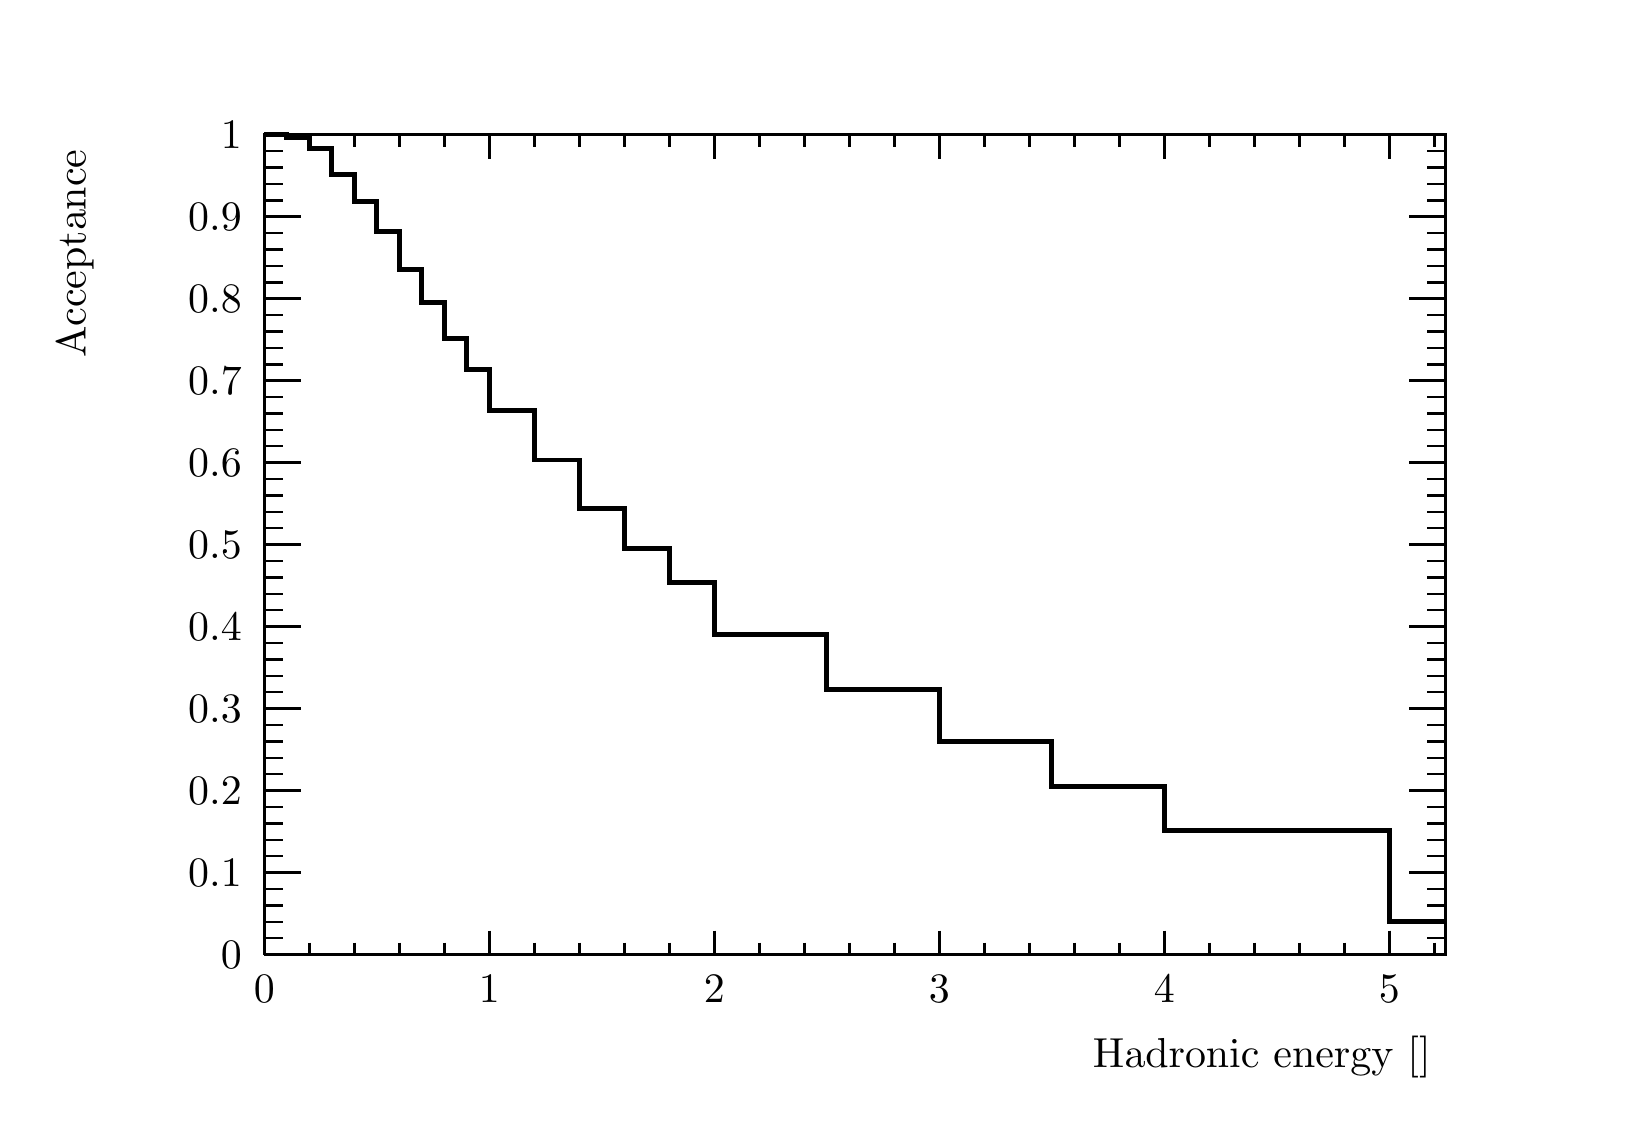
\begin{tikzpicture}
\pgfdeclareplotmark{cross} {
\pgfpathmoveto{\pgfpoint{-0.3\pgfplotmarksize}{\pgfplotmarksize}}
\pgfpathlineto{\pgfpoint{+0.3\pgfplotmarksize}{\pgfplotmarksize}}
\pgfpathlineto{\pgfpoint{+0.3\pgfplotmarksize}{0.3\pgfplotmarksize}}
\pgfpathlineto{\pgfpoint{+1\pgfplotmarksize}{0.3\pgfplotmarksize}}
\pgfpathlineto{\pgfpoint{+1\pgfplotmarksize}{-0.3\pgfplotmarksize}}
\pgfpathlineto{\pgfpoint{+0.3\pgfplotmarksize}{-0.3\pgfplotmarksize}}
\pgfpathlineto{\pgfpoint{+0.3\pgfplotmarksize}{-1.\pgfplotmarksize}}
\pgfpathlineto{\pgfpoint{-0.3\pgfplotmarksize}{-1.\pgfplotmarksize}}
\pgfpathlineto{\pgfpoint{-0.3\pgfplotmarksize}{-0.3\pgfplotmarksize}}
\pgfpathlineto{\pgfpoint{-1.\pgfplotmarksize}{-0.3\pgfplotmarksize}}
\pgfpathlineto{\pgfpoint{-1.\pgfplotmarksize}{0.3\pgfplotmarksize}}
\pgfpathlineto{\pgfpoint{-0.3\pgfplotmarksize}{0.3\pgfplotmarksize}}
\pgfpathclose
\pgfusepathqstroke
}
\pgfdeclareplotmark{cross*} {
\pgfpathmoveto{\pgfpoint{-0.3\pgfplotmarksize}{\pgfplotmarksize}}
\pgfpathlineto{\pgfpoint{+0.3\pgfplotmarksize}{\pgfplotmarksize}}
\pgfpathlineto{\pgfpoint{+0.3\pgfplotmarksize}{0.3\pgfplotmarksize}}
\pgfpathlineto{\pgfpoint{+1\pgfplotmarksize}{0.3\pgfplotmarksize}}
\pgfpathlineto{\pgfpoint{+1\pgfplotmarksize}{-0.3\pgfplotmarksize}}
\pgfpathlineto{\pgfpoint{+0.3\pgfplotmarksize}{-0.3\pgfplotmarksize}}
\pgfpathlineto{\pgfpoint{+0.3\pgfplotmarksize}{-1.\pgfplotmarksize}}
\pgfpathlineto{\pgfpoint{-0.3\pgfplotmarksize}{-1.\pgfplotmarksize}}
\pgfpathlineto{\pgfpoint{-0.3\pgfplotmarksize}{-0.3\pgfplotmarksize}}
\pgfpathlineto{\pgfpoint{-1.\pgfplotmarksize}{-0.3\pgfplotmarksize}}
\pgfpathlineto{\pgfpoint{-1.\pgfplotmarksize}{0.3\pgfplotmarksize}}
\pgfpathlineto{\pgfpoint{-0.3\pgfplotmarksize}{0.3\pgfplotmarksize}}
\pgfpathclose
\pgfusepathqfillstroke
}
\pgfdeclareplotmark{newstar} {
\pgfpathmoveto{\pgfqpoint{0pt}{\pgfplotmarksize}}
\pgfpathlineto{\pgfqpointpolar{44}{0.5\pgfplotmarksize}}
\pgfpathlineto{\pgfqpointpolar{18}{\pgfplotmarksize}}
\pgfpathlineto{\pgfqpointpolar{-20}{0.5\pgfplotmarksize}}
\pgfpathlineto{\pgfqpointpolar{-54}{\pgfplotmarksize}}
\pgfpathlineto{\pgfqpointpolar{-90}{0.5\pgfplotmarksize}}
\pgfpathlineto{\pgfqpointpolar{234}{\pgfplotmarksize}}
\pgfpathlineto{\pgfqpointpolar{198}{0.5\pgfplotmarksize}}
\pgfpathlineto{\pgfqpointpolar{162}{\pgfplotmarksize}}
\pgfpathlineto{\pgfqpointpolar{134}{0.5\pgfplotmarksize}}
\pgfpathclose
\pgfusepathqstroke
}
\pgfdeclareplotmark{newstar*} {
\pgfpathmoveto{\pgfqpoint{0pt}{\pgfplotmarksize}}
\pgfpathlineto{\pgfqpointpolar{44}{0.5\pgfplotmarksize}}
\pgfpathlineto{\pgfqpointpolar{18}{\pgfplotmarksize}}
\pgfpathlineto{\pgfqpointpolar{-20}{0.5\pgfplotmarksize}}
\pgfpathlineto{\pgfqpointpolar{-54}{\pgfplotmarksize}}
\pgfpathlineto{\pgfqpointpolar{-90}{0.5\pgfplotmarksize}}
\pgfpathlineto{\pgfqpointpolar{234}{\pgfplotmarksize}}
\pgfpathlineto{\pgfqpointpolar{198}{0.5\pgfplotmarksize}}
\pgfpathlineto{\pgfqpointpolar{162}{\pgfplotmarksize}}
\pgfpathlineto{\pgfqpointpolar{134}{0.5\pgfplotmarksize}}
\pgfpathclose
\pgfusepathqfillstroke
}
\definecolor{c}{rgb}{1,1,1};
\draw [color=c, fill=c] (0,0) rectangle (20,13.5227);
\draw [color=c, fill=c] (3,1.75795) rectangle (18,12.1705);
\definecolor{c}{rgb}{0,0,0};
\draw [c,line width=0.9] (3,1.75795) -- (3,12.1705) -- (18,12.1705) -- (18,1.75795) -- (3,1.75795);
\definecolor{c}{rgb}{1,1,1};
\draw [color=c, fill=c] (3,1.75795) rectangle (18,12.1705);
\definecolor{c}{rgb}{0,0,0};
\draw [c,line width=0.9] (3,1.75795) -- (3,12.1705) -- (18,12.1705) -- (18,1.75795) -- (3,1.75795);
\draw [c,line width=1.8] (3,12.1669) -- (3.28571,12.1669) -- (3.28571,12.1337) -- (3.57143,12.1337) -- (3.57143,11.9974) -- (3.85714,11.9974) -- (3.85714,11.6598) -- (4.14286,11.6598) -- (4.14286,11.3159) -- (4.42857,11.3159) -- (4.42857,10.9376) --
 (4.71429,10.9376) -- (4.71429,10.4567) -- (5,10.4567) -- (5,10.038) -- (5.28571,10.038) -- (5.28571,9.58251) -- (5.57143,9.58251) -- (5.57143,9.19266) -- (5.85714,9.19266) -- (5.85714,8.6728) -- (6.42857,8.6728) -- (6.42857,8.03916) -- (7,8.03916)
 -- (7,7.41873) -- (7.57143,7.41873) -- (7.57143,6.91137) -- (8.14286,6.91137) -- (8.14286,6.48146) -- (8.71429,6.48146) -- (8.71429,5.82387) -- (10.1429,5.82387) -- (10.1429,5.12498) -- (11.5714,5.12498) -- (11.5714,4.45809) -- (13,4.45809) --
 (13,3.88768) -- (14.4286,3.88768) -- (14.4286,3.33927) -- (17.2857,3.33927) -- (17.2857,2.18148) -- (18,2.18148);
\draw [c,line width=0.9] (3,1.75795) -- (18,1.75795);
\draw [c,line width=0.9] (3,2.06222) -- (3,1.75795);
\draw [c,line width=0.9] (3.57143,1.91009) -- (3.57143,1.75795);
\draw [c,line width=0.9] (4.14286,1.91009) -- (4.14286,1.75795);
\draw [c,line width=0.9] (4.71429,1.91009) -- (4.71429,1.75795);
\draw [c,line width=0.9] (5.28571,1.91009) -- (5.28571,1.75795);
\draw [c,line width=0.9] (5.85714,2.06222) -- (5.85714,1.75795);
\draw [c,line width=0.9] (6.42857,1.91009) -- (6.42857,1.75795);
\draw [c,line width=0.9] (7,1.91009) -- (7,1.75795);
\draw [c,line width=0.9] (7.57143,1.91009) -- (7.57143,1.75795);
\draw [c,line width=0.9] (8.14286,1.91009) -- (8.14286,1.75795);
\draw [c,line width=0.9] (8.71429,2.06222) -- (8.71429,1.75795);
\draw [c,line width=0.9] (9.28571,1.91009) -- (9.28571,1.75795);
\draw [c,line width=0.9] (9.85714,1.91009) -- (9.85714,1.75795);
\draw [c,line width=0.9] (10.4286,1.91009) -- (10.4286,1.75795);
\draw [c,line width=0.9] (11,1.91009) -- (11,1.75795);
\draw [c,line width=0.9] (11.5714,2.06222) -- (11.5714,1.75795);
\draw [c,line width=0.9] (12.1429,1.91009) -- (12.1429,1.75795);
\draw [c,line width=0.9] (12.7143,1.91009) -- (12.7143,1.75795);
\draw [c,line width=0.9] (13.2857,1.91009) -- (13.2857,1.75795);
\draw [c,line width=0.9] (13.8571,1.91009) -- (13.8571,1.75795);
\draw [c,line width=0.9] (14.4286,2.06222) -- (14.4286,1.75795);
\draw [c,line width=0.9] (15,1.91009) -- (15,1.75795);
\draw [c,line width=0.9] (15.5714,1.91009) -- (15.5714,1.75795);
\draw [c,line width=0.9] (16.1429,1.91009) -- (16.1429,1.75795);
\draw [c,line width=0.9] (16.7143,1.91009) -- (16.7143,1.75795);
\draw [c,line width=0.9] (17.2857,2.06222) -- (17.2857,1.75795);
\draw [c,line width=0.9] (17.2857,2.06222) -- (17.2857,1.75795);
\draw [c,line width=0.9] (17.8571,1.91009) -- (17.8571,1.75795);
\draw [anchor=base] (3,1.14943) node[scale=1.5143, color=c, rotate=0]{0};
\draw [anchor=base] (5.85714,1.14943) node[scale=1.5143, color=c, rotate=0]{1};
\draw [anchor=base] (8.71429,1.14943) node[scale=1.5143, color=c, rotate=0]{2};
\draw [anchor=base] (11.5714,1.14943) node[scale=1.5143, color=c, rotate=0]{3};
\draw [anchor=base] (14.4286,1.14943) node[scale=1.5143, color=c, rotate=0]{4};
\draw [anchor=base] (17.2857,1.14943) node[scale=1.5143, color=c, rotate=0]{5};
\draw [anchor= east] (18,0.459773) node[scale=1.5143, color=c, rotate=0]{Hadronic energy [\si{\GeV}] };
\draw [c,line width=0.9] (3,12.1705) -- (18,12.1705);
\draw [c,line width=0.9] (3,11.8662) -- (3,12.1705);
\draw [c,line width=0.9] (3.57143,12.0183) -- (3.57143,12.1705);
\draw [c,line width=0.9] (4.14286,12.0183) -- (4.14286,12.1705);
\draw [c,line width=0.9] (4.71429,12.0183) -- (4.71429,12.1705);
\draw [c,line width=0.9] (5.28571,12.0183) -- (5.28571,12.1705);
\draw [c,line width=0.9] (5.85714,11.8662) -- (5.85714,12.1705);
\draw [c,line width=0.9] (6.42857,12.0183) -- (6.42857,12.1705);
\draw [c,line width=0.9] (7,12.0183) -- (7,12.1705);
\draw [c,line width=0.9] (7.57143,12.0183) -- (7.57143,12.1705);
\draw [c,line width=0.9] (8.14286,12.0183) -- (8.14286,12.1705);
\draw [c,line width=0.9] (8.71429,11.8662) -- (8.71429,12.1705);
\draw [c,line width=0.9] (9.28571,12.0183) -- (9.28571,12.1705);
\draw [c,line width=0.9] (9.85714,12.0183) -- (9.85714,12.1705);
\draw [c,line width=0.9] (10.4286,12.0183) -- (10.4286,12.1705);
\draw [c,line width=0.9] (11,12.0183) -- (11,12.1705);
\draw [c,line width=0.9] (11.5714,11.8662) -- (11.5714,12.1705);
\draw [c,line width=0.9] (12.1429,12.0183) -- (12.1429,12.1705);
\draw [c,line width=0.9] (12.7143,12.0183) -- (12.7143,12.1705);
\draw [c,line width=0.9] (13.2857,12.0183) -- (13.2857,12.1705);
\draw [c,line width=0.9] (13.8571,12.0183) -- (13.8571,12.1705);
\draw [c,line width=0.9] (14.4286,11.8662) -- (14.4286,12.1705);
\draw [c,line width=0.9] (15,12.0183) -- (15,12.1705);
\draw [c,line width=0.9] (15.5714,12.0183) -- (15.5714,12.1705);
\draw [c,line width=0.9] (16.1429,12.0183) -- (16.1429,12.1705);
\draw [c,line width=0.9] (16.7143,12.0183) -- (16.7143,12.1705);
\draw [c,line width=0.9] (17.2857,11.8662) -- (17.2857,12.1705);
\draw [c,line width=0.9] (17.2857,11.8662) -- (17.2857,12.1705);
\draw [c,line width=0.9] (17.8571,12.0183) -- (17.8571,12.1705);
\draw [c,line width=0.9] (3,1.75795) -- (3,12.1705);
\draw [c,line width=0.9] (3.462,1.75795) -- (3,1.75795);
\draw [c,line width=0.9] (3.231,1.9662) -- (3,1.9662);
\draw [c,line width=0.9] (3.231,2.17445) -- (3,2.17445);
\draw [c,line width=0.9] (3.231,2.3827) -- (3,2.3827);
\draw [c,line width=0.9] (3.231,2.59095) -- (3,2.59095);
\draw [c,line width=0.9] (3.462,2.7992) -- (3,2.7992);
\draw [c,line width=0.9] (3.231,3.00745) -- (3,3.00745);
\draw [c,line width=0.9] (3.231,3.2157) -- (3,3.2157);
\draw [c,line width=0.9] (3.231,3.42395) -- (3,3.42395);
\draw [c,line width=0.9] (3.231,3.6322) -- (3,3.6322);
\draw [c,line width=0.9] (3.462,3.84045) -- (3,3.84045);
\draw [c,line width=0.9] (3.231,4.0487) -- (3,4.0487);
\draw [c,line width=0.9] (3.231,4.25695) -- (3,4.25695);
\draw [c,line width=0.9] (3.231,4.4652) -- (3,4.4652);
\draw [c,line width=0.9] (3.231,4.67345) -- (3,4.67345);
\draw [c,line width=0.9] (3.462,4.8817) -- (3,4.8817);
\draw [c,line width=0.9] (3.231,5.08995) -- (3,5.08995);
\draw [c,line width=0.9] (3.231,5.2982) -- (3,5.2982);
\draw [c,line width=0.9] (3.231,5.50645) -- (3,5.50645);
\draw [c,line width=0.9] (3.231,5.7147) -- (3,5.7147);
\draw [c,line width=0.9] (3.462,5.92295) -- (3,5.92295);
\draw [c,line width=0.9] (3.231,6.1312) -- (3,6.1312);
\draw [c,line width=0.9] (3.231,6.33945) -- (3,6.33945);
\draw [c,line width=0.9] (3.231,6.5477) -- (3,6.5477);
\draw [c,line width=0.9] (3.231,6.75595) -- (3,6.75595);
\draw [c,line width=0.9] (3.462,6.9642) -- (3,6.9642);
\draw [c,line width=0.9] (3.231,7.17245) -- (3,7.17245);
\draw [c,line width=0.9] (3.231,7.3807) -- (3,7.3807);
\draw [c,line width=0.9] (3.231,7.58895) -- (3,7.58895);
\draw [c,line width=0.9] (3.231,7.7972) -- (3,7.7972);
\draw [c,line width=0.9] (3.462,8.00545) -- (3,8.00545);
\draw [c,line width=0.9] (3.231,8.2137) -- (3,8.2137);
\draw [c,line width=0.9] (3.231,8.42195) -- (3,8.42195);
\draw [c,line width=0.9] (3.231,8.6302) -- (3,8.6302);
\draw [c,line width=0.9] (3.231,8.83845) -- (3,8.83845);
\draw [c,line width=0.9] (3.462,9.0467) -- (3,9.0467);
\draw [c,line width=0.9] (3.231,9.25495) -- (3,9.25495);
\draw [c,line width=0.9] (3.231,9.4632) -- (3,9.4632);
\draw [c,line width=0.9] (3.231,9.67145) -- (3,9.67145);
\draw [c,line width=0.9] (3.231,9.8797) -- (3,9.8797);
\draw [c,line width=0.9] (3.462,10.088) -- (3,10.088);
\draw [c,line width=0.9] (3.231,10.2962) -- (3,10.2962);
\draw [c,line width=0.9] (3.231,10.5045) -- (3,10.5045);
\draw [c,line width=0.9] (3.231,10.7127) -- (3,10.7127);
\draw [c,line width=0.9] (3.231,10.921) -- (3,10.921);
\draw [c,line width=0.9] (3.462,11.1292) -- (3,11.1292);
\draw [c,line width=0.9] (3.231,11.3375) -- (3,11.3375);
\draw [c,line width=0.9] (3.231,11.5457) -- (3,11.5457);
\draw [c,line width=0.9] (3.231,11.754) -- (3,11.754);
\draw [c,line width=0.9] (3.231,11.9622) -- (3,11.9622);
\draw [c,line width=0.9] (3.462,12.1705) -- (3,12.1705);
\draw [anchor= east] (2.9,1.75795) node[scale=1.5143, color=c, rotate=0]{0};
\draw [anchor= east] (2.9,2.7992) node[scale=1.5143, color=c, rotate=0]{0.1};
\draw [anchor= east] (2.9,3.84045) node[scale=1.5143, color=c, rotate=0]{0.2};
\draw [anchor= east] (2.9,4.8817) node[scale=1.5143, color=c, rotate=0]{0.3};
\draw [anchor= east] (2.9,5.92295) node[scale=1.5143, color=c, rotate=0]{0.4};
\draw [anchor= east] (2.9,6.9642) node[scale=1.5143, color=c, rotate=0]{0.5};
\draw [anchor= east] (2.9,8.00545) node[scale=1.5143, color=c, rotate=0]{0.6};
\draw [anchor= east] (2.9,9.0467) node[scale=1.5143, color=c, rotate=0]{0.7};
\draw [anchor= east] (2.9,10.088) node[scale=1.5143, color=c, rotate=0]{0.8};
\draw [anchor= east] (2.9,11.1292) node[scale=1.5143, color=c, rotate=0]{0.9};
\draw [anchor= east] (2.9,12.1705) node[scale=1.5143, color=c, rotate=0]{1};
\draw [anchor= east] (0.6,12.1705) node[scale=1.5143, color=c, rotate=90]{Acceptance};
\draw [c,line width=0.9] (18,1.75795) -- (18,12.1705);
\draw [c,line width=0.9] (17.538,1.75795) -- (18,1.75795);
\draw [c,line width=0.9] (17.769,1.9662) -- (18,1.9662);
\draw [c,line width=0.9] (17.769,2.17445) -- (18,2.17445);
\draw [c,line width=0.9] (17.769,2.3827) -- (18,2.3827);
\draw [c,line width=0.9] (17.769,2.59095) -- (18,2.59095);
\draw [c,line width=0.9] (17.538,2.7992) -- (18,2.7992);
\draw [c,line width=0.9] (17.769,3.00745) -- (18,3.00745);
\draw [c,line width=0.9] (17.769,3.2157) -- (18,3.2157);
\draw [c,line width=0.9] (17.769,3.42395) -- (18,3.42395);
\draw [c,line width=0.9] (17.769,3.6322) -- (18,3.6322);
\draw [c,line width=0.9] (17.538,3.84045) -- (18,3.84045);
\draw [c,line width=0.9] (17.769,4.0487) -- (18,4.0487);
\draw [c,line width=0.9] (17.769,4.25695) -- (18,4.25695);
\draw [c,line width=0.9] (17.769,4.4652) -- (18,4.4652);
\draw [c,line width=0.9] (17.769,4.67345) -- (18,4.67345);
\draw [c,line width=0.9] (17.538,4.8817) -- (18,4.8817);
\draw [c,line width=0.9] (17.769,5.08995) -- (18,5.08995);
\draw [c,line width=0.9] (17.769,5.2982) -- (18,5.2982);
\draw [c,line width=0.9] (17.769,5.50645) -- (18,5.50645);
\draw [c,line width=0.9] (17.769,5.7147) -- (18,5.7147);
\draw [c,line width=0.9] (17.538,5.92295) -- (18,5.92295);
\draw [c,line width=0.9] (17.769,6.1312) -- (18,6.1312);
\draw [c,line width=0.9] (17.769,6.33945) -- (18,6.33945);
\draw [c,line width=0.9] (17.769,6.5477) -- (18,6.5477);
\draw [c,line width=0.9] (17.769,6.75595) -- (18,6.75595);
\draw [c,line width=0.9] (17.538,6.9642) -- (18,6.9642);
\draw [c,line width=0.9] (17.769,7.17245) -- (18,7.17245);
\draw [c,line width=0.9] (17.769,7.3807) -- (18,7.3807);
\draw [c,line width=0.9] (17.769,7.58895) -- (18,7.58895);
\draw [c,line width=0.9] (17.769,7.7972) -- (18,7.7972);
\draw [c,line width=0.9] (17.538,8.00545) -- (18,8.00545);
\draw [c,line width=0.9] (17.769,8.2137) -- (18,8.2137);
\draw [c,line width=0.9] (17.769,8.42195) -- (18,8.42195);
\draw [c,line width=0.9] (17.769,8.6302) -- (18,8.6302);
\draw [c,line width=0.9] (17.769,8.83845) -- (18,8.83845);
\draw [c,line width=0.9] (17.538,9.0467) -- (18,9.0467);
\draw [c,line width=0.9] (17.769,9.25495) -- (18,9.25495);
\draw [c,line width=0.9] (17.769,9.4632) -- (18,9.4632);
\draw [c,line width=0.9] (17.769,9.67145) -- (18,9.67145);
\draw [c,line width=0.9] (17.769,9.8797) -- (18,9.8797);
\draw [c,line width=0.9] (17.538,10.088) -- (18,10.088);
\draw [c,line width=0.9] (17.769,10.2962) -- (18,10.2962);
\draw [c,line width=0.9] (17.769,10.5045) -- (18,10.5045);
\draw [c,line width=0.9] (17.769,10.7127) -- (18,10.7127);
\draw [c,line width=0.9] (17.769,10.921) -- (18,10.921);
\draw [c,line width=0.9] (17.538,11.1292) -- (18,11.1292);
\draw [c,line width=0.9] (17.769,11.3375) -- (18,11.3375);
\draw [c,line width=0.9] (17.769,11.5457) -- (18,11.5457);
\draw [c,line width=0.9] (17.769,11.754) -- (18,11.754);
\draw [c,line width=0.9] (17.769,11.9622) -- (18,11.9622);
\draw [c,line width=0.9] (17.538,12.1705) -- (18,12.1705);
\end{tikzpicture}

		\end{adjustbox}
	\end{minipage}
	\caption[Muonic and hadronic acceptance for CC neutrino interactions in ND-LAr]{Left: Muonic acceptance for CC muon neutrino interactions in ND-LAr as a function of transverse and longitudinal muon momentum. Right: Hadronic acceptance for CC muon neutrino interactions in ND-LAr as a function of true hadronic energy. Both from~\cite{Abi:2020qib}.}
	\label{fig:ndAcceptance}
\end{figure}

The uncertainty on the muon and hadron acceptance is produced from the respective plots in \citefig{fig:ndAcceptance} with a higher uncertainty in regions where the acceptance is rapidly changing and thus vulnerable to mismodelling.

Unlike their FD counterparts, the ND detector parameters are not allowed to vary in the fit.
Instead, they are incorporated into a covariance matrix.
This covariance matrix is formed by throwing all ND detector uncertainties simultaneously according to their documented uncertainties and comparing the resulting spectra with the nominal prediction.
The bin-to-bin covariance is then determined using these comparisons.

This method differs from that used for the FD due to significant differences in the development of the ND and FD simulation.
The FD simulation uses a full detector simulation along with a fully simulated energy reconstruction based upon the Pandora toolkit~\cite{pandora}.
The ND simulation is much simpler. 
Although neutrino interactions are simulated within the ND volume in the same manner as the FD, with the interaction products being propagated through the detector using a Geant4-based model~\cite{geant}, sufficient reconstruction software has not yet been developed for ND-LAr.
Therefore a parametrised reconstruction is used, taking as inputs the true simulated energy deposits.
The high statistics of the ND, combined with this simplified detector model, leads to over-constraining of the ND detector parameters, if included as nuisance parameters.
The decision is therefore made to use the above method for the ND detector systematics.
This method is unnecessary in the FD where a full reconstruction is used.

\section{DUNE sensitivites}
\label{sec:dune_lbl:sensitivities}

\subsection{CAFAna}
\label{sec:dune_lbl:sensitivities:cafana}

DUNE's oscillation sensitivities are computed using the CAFAna package, further details of which are given here.
This framework derives its name from the input files which are known as Common Analysis Files (CAFs).
These files typically contain higher level reconstructed variables typically used by analysers and consist of a \texttt{ROOT}~\cite{root} \texttt{TTree}, each entry of which represents a suspected neutrino interaction~\cite{backhouse2015}.

CAFAna was originally developed for the NOvA oscillation analysis but has since been ported for use by both the DUNE and Short-Baseline Neutrino (SBN) collaborations~\cite{cafana}.
Its primary functions are the creation of histograms from the input files and the derivation of oscillation parameters from those histograms.

Additionally, CAFAna allows the effect of systematic variations on each output histogram to be viewed. 
These systematics can take the form of either reweightings or bin-to-bin shifting of events and are implemented as 1D response functions for each analysis bin.
The response functions for bin-to-bin shifts are constructed by taking the calculating the content of each bin at $\pm 1 \sigma$, $\pm 2 \sigma$ and $\pm 3 \sigma$ and then performing a cubic interpolation between these points.

In terms of CAFAna's fitting components, a frequentist approach is adopted with the minimisation being performed by the \texttt{MINUIT}~\cite{minuit} package.

The entire framework is written in C++ and may be controlled by the user through \texttt{ROOT} macros.

\subsection{General sensitivity methods}
\label{sec:dune_lbl:sensitivities:general}

Oscillation sensitivities are computed by simultaneously fitting the oscillation parameters and nuisance parameters to four FD spectra (\numu disappearance, \anumu disappearance, \nue appearance and \anue appearance) and the nuisance parameters to the two ND spectra (\numu unoscillated and \anumu unoscillated).
In the current DUNE analysis the intrinsic \nue beam flux is not constrained by the ND due to the simplicity of the ND reconstruction.
However, in a real analysis it is expected that this would be included.

Examples of the four FD event rates as a function of reconstructed neutrino energy are shown in \citefig{fig:fdEventRatesWithErrorBand}.
In each case, the $\pm1\sigma$ systematic error band is also shown in red.
Furthermore, for the appearance samples, the different event rates resulting from different neutrino mass hierarchies and values of \dcp are shown, while for the disappearance samples the effect of varying \thetai{23} is shown.
One can see that the systematic errors are significant for all samples across the energy range.
The variation in the appearance rates with \dcp is larger than the expected variation due to the systematics.
However, the systematic uncertainty is comparable to the expected \thetai{23} variation, indicating that tight constraints of these systematics will be required to make precision measurements of this variable.

\begin{figure}
	\begin{minipage}[t]{.5\linewidth}
		\begin{adjustbox}{max totalsize=\linewidth, center}
			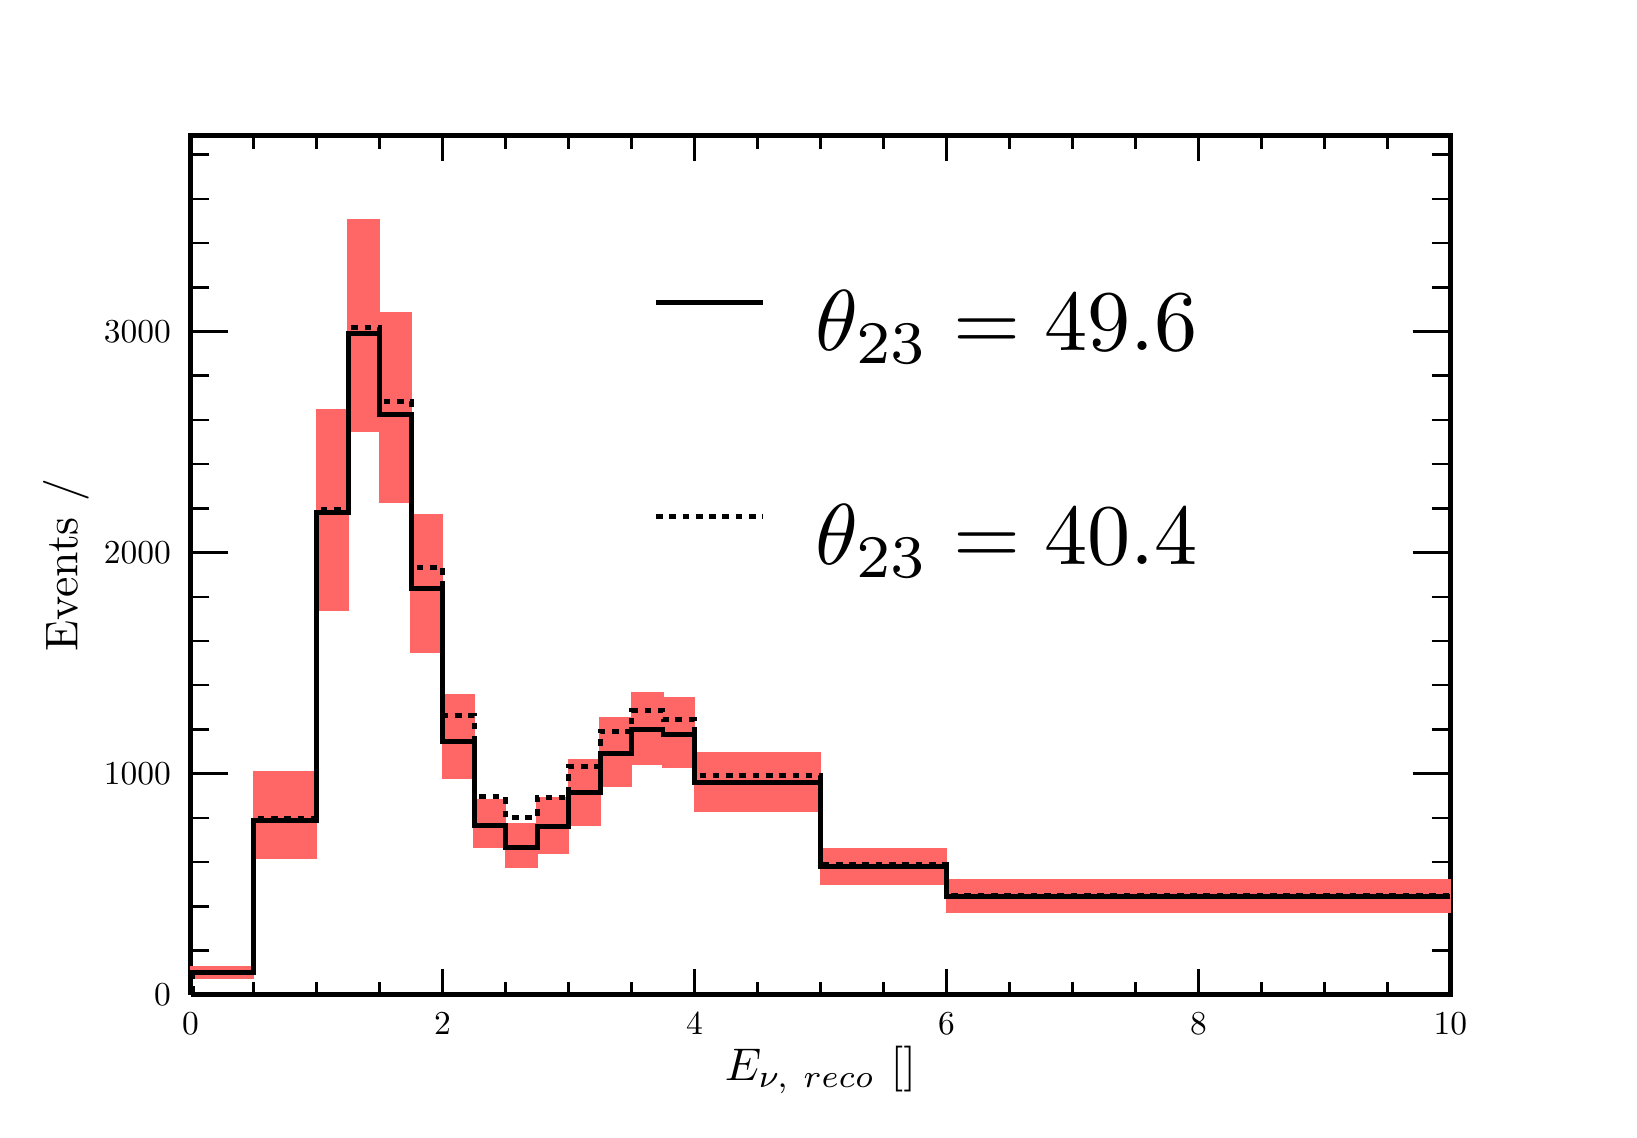
\begin{tikzpicture}
\pgfdeclareplotmark{cross} {
\pgfpathmoveto{\pgfpoint{-0.3\pgfplotmarksize}{\pgfplotmarksize}}
\pgfpathlineto{\pgfpoint{+0.3\pgfplotmarksize}{\pgfplotmarksize}}
\pgfpathlineto{\pgfpoint{+0.3\pgfplotmarksize}{0.3\pgfplotmarksize}}
\pgfpathlineto{\pgfpoint{+1\pgfplotmarksize}{0.3\pgfplotmarksize}}
\pgfpathlineto{\pgfpoint{+1\pgfplotmarksize}{-0.3\pgfplotmarksize}}
\pgfpathlineto{\pgfpoint{+0.3\pgfplotmarksize}{-0.3\pgfplotmarksize}}
\pgfpathlineto{\pgfpoint{+0.3\pgfplotmarksize}{-1.\pgfplotmarksize}}
\pgfpathlineto{\pgfpoint{-0.3\pgfplotmarksize}{-1.\pgfplotmarksize}}
\pgfpathlineto{\pgfpoint{-0.3\pgfplotmarksize}{-0.3\pgfplotmarksize}}
\pgfpathlineto{\pgfpoint{-1.\pgfplotmarksize}{-0.3\pgfplotmarksize}}
\pgfpathlineto{\pgfpoint{-1.\pgfplotmarksize}{0.3\pgfplotmarksize}}
\pgfpathlineto{\pgfpoint{-0.3\pgfplotmarksize}{0.3\pgfplotmarksize}}
\pgfpathclose
\pgfusepathqstroke
}
\pgfdeclareplotmark{cross*} {
\pgfpathmoveto{\pgfpoint{-0.3\pgfplotmarksize}{\pgfplotmarksize}}
\pgfpathlineto{\pgfpoint{+0.3\pgfplotmarksize}{\pgfplotmarksize}}
\pgfpathlineto{\pgfpoint{+0.3\pgfplotmarksize}{0.3\pgfplotmarksize}}
\pgfpathlineto{\pgfpoint{+1\pgfplotmarksize}{0.3\pgfplotmarksize}}
\pgfpathlineto{\pgfpoint{+1\pgfplotmarksize}{-0.3\pgfplotmarksize}}
\pgfpathlineto{\pgfpoint{+0.3\pgfplotmarksize}{-0.3\pgfplotmarksize}}
\pgfpathlineto{\pgfpoint{+0.3\pgfplotmarksize}{-1.\pgfplotmarksize}}
\pgfpathlineto{\pgfpoint{-0.3\pgfplotmarksize}{-1.\pgfplotmarksize}}
\pgfpathlineto{\pgfpoint{-0.3\pgfplotmarksize}{-0.3\pgfplotmarksize}}
\pgfpathlineto{\pgfpoint{-1.\pgfplotmarksize}{-0.3\pgfplotmarksize}}
\pgfpathlineto{\pgfpoint{-1.\pgfplotmarksize}{0.3\pgfplotmarksize}}
\pgfpathlineto{\pgfpoint{-0.3\pgfplotmarksize}{0.3\pgfplotmarksize}}
\pgfpathclose
\pgfusepathqfillstroke
}
\pgfdeclareplotmark{newstar} {
\pgfpathmoveto{\pgfqpoint{0pt}{\pgfplotmarksize}}
\pgfpathlineto{\pgfqpointpolar{44}{0.5\pgfplotmarksize}}
\pgfpathlineto{\pgfqpointpolar{18}{\pgfplotmarksize}}
\pgfpathlineto{\pgfqpointpolar{-20}{0.5\pgfplotmarksize}}
\pgfpathlineto{\pgfqpointpolar{-54}{\pgfplotmarksize}}
\pgfpathlineto{\pgfqpointpolar{-90}{0.5\pgfplotmarksize}}
\pgfpathlineto{\pgfqpointpolar{234}{\pgfplotmarksize}}
\pgfpathlineto{\pgfqpointpolar{198}{0.5\pgfplotmarksize}}
\pgfpathlineto{\pgfqpointpolar{162}{\pgfplotmarksize}}
\pgfpathlineto{\pgfqpointpolar{134}{0.5\pgfplotmarksize}}
\pgfpathclose
\pgfusepathqstroke
}
\pgfdeclareplotmark{newstar*} {
\pgfpathmoveto{\pgfqpoint{0pt}{\pgfplotmarksize}}
\pgfpathlineto{\pgfqpointpolar{44}{0.5\pgfplotmarksize}}
\pgfpathlineto{\pgfqpointpolar{18}{\pgfplotmarksize}}
\pgfpathlineto{\pgfqpointpolar{-20}{0.5\pgfplotmarksize}}
\pgfpathlineto{\pgfqpointpolar{-54}{\pgfplotmarksize}}
\pgfpathlineto{\pgfqpointpolar{-90}{0.5\pgfplotmarksize}}
\pgfpathlineto{\pgfqpointpolar{234}{\pgfplotmarksize}}
\pgfpathlineto{\pgfqpointpolar{198}{0.5\pgfplotmarksize}}
\pgfpathlineto{\pgfqpointpolar{162}{\pgfplotmarksize}}
\pgfpathlineto{\pgfqpointpolar{134}{0.5\pgfplotmarksize}}
\pgfpathclose
\pgfusepathqfillstroke
}
\definecolor{c}{rgb}{0.999,0.999,0.999};
\draw [color=c, fill=c] (0,0) rectangle (20,13.639);
\draw [color=c, fill=c] (2,1.3639) rectangle (18,12.2751);
\definecolor{c}{rgb}{0,0,0};
\draw [c,line width=1.8] (2,1.3639) -- (2,12.2751) -- (18,12.2751) -- (18,1.3639) -- (2,1.3639);
\definecolor{c}{rgb}{0.999,0.999,0.999};
\draw [color=c, fill=c] (2,1.3639) rectangle (18,12.2751);
\definecolor{c}{rgb}{0,0,0};
\draw [c,line width=1.8] (2,1.3639) -- (2,12.2751) -- (18,12.2751) -- (18,1.3639) -- (2,1.3639);
\draw [c,line width=1.8] (2,1.64499) -- (2.8,1.64499) -- (2.8,3.58066) -- (3.6,3.58066) -- (3.6,7.48952) -- (4,7.48952) -- (4,9.75711) -- (4.4,9.75711) -- (4.4,8.72912) -- (4.8,8.72912) -- (4.8,6.52389) -- (5.2,6.52389) -- (5.2,4.58459) --
 (5.6,4.58459) -- (5.6,3.51089) -- (6,3.51089) -- (6,3.23684) -- (6.4,3.23684) -- (6.4,3.5047) -- (6.8,3.5047) -- (6.8,3.93032) -- (7.2,3.93032) -- (7.2,4.42465) -- (7.6,4.42465) -- (7.6,4.73254) -- (8,4.73254) -- (8,4.6717) -- (8.4,4.6717) --
 (8.4,4.05577) -- (10,4.05577) -- (10,2.98825) -- (11.6,2.98825) -- (11.6,2.61432) -- (18,2.61432);
\draw [c,line width=0.9] (2,1.3639) -- (18,1.3639);
\draw [c,line width=0.9] (2,1.69123) -- (2,1.3639);
\draw [c,line width=0.9] (2.8,1.52756) -- (2.8,1.3639);
\draw [c,line width=0.9] (3.6,1.52756) -- (3.6,1.3639);
\draw [c,line width=0.9] (4.4,1.52756) -- (4.4,1.3639);
\draw [c,line width=0.9] (5.2,1.69123) -- (5.2,1.3639);
\draw [c,line width=0.9] (6,1.52756) -- (6,1.3639);
\draw [c,line width=0.9] (6.8,1.52756) -- (6.8,1.3639);
\draw [c,line width=0.9] (7.6,1.52756) -- (7.6,1.3639);
\draw [c,line width=0.9] (8.4,1.69123) -- (8.4,1.3639);
\draw [c,line width=0.9] (9.2,1.52756) -- (9.2,1.3639);
\draw [c,line width=0.9] (10,1.52756) -- (10,1.3639);
\draw [c,line width=0.9] (10.8,1.52756) -- (10.8,1.3639);
\draw [c,line width=0.9] (11.6,1.69123) -- (11.6,1.3639);
\draw [c,line width=0.9] (12.4,1.52756) -- (12.4,1.3639);
\draw [c,line width=0.9] (13.2,1.52756) -- (13.2,1.3639);
\draw [c,line width=0.9] (14,1.52756) -- (14,1.3639);
\draw [c,line width=0.9] (14.8,1.69123) -- (14.8,1.3639);
\draw [c,line width=0.9] (15.6,1.52756) -- (15.6,1.3639);
\draw [c,line width=0.9] (16.4,1.52756) -- (16.4,1.3639);
\draw [c,line width=0.9] (17.2,1.52756) -- (17.2,1.3639);
\draw [c,line width=0.9] (18,1.69123) -- (18,1.3639);
\draw [anchor=base] (2,0.859255) node[scale=1.20912, color=c, rotate=0]{0};
\draw [anchor=base] (5.2,0.859255) node[scale=1.20912, color=c, rotate=0]{2};
\draw [anchor=base] (8.4,0.859255) node[scale=1.20912, color=c, rotate=0]{4};
\draw [anchor=base] (11.6,0.859255) node[scale=1.20912, color=c, rotate=0]{6};
\draw [anchor=base] (14.8,0.859255) node[scale=1.20912, color=c, rotate=0]{8};
\draw [anchor=base] (18,0.859255) node[scale=1.20912, color=c, rotate=0]{10};
\draw (10,0.403714) node[scale=1.65459, color=c, rotate=0]{$E_{\nu,~\text{reco}}$ [\si{\GeV}]};
\draw [c,line width=0.9] (2,12.2751) -- (18,12.2751);
\draw [c,line width=0.9] (2,11.9477) -- (2,12.2751);
\draw [c,line width=0.9] (2.8,12.1114) -- (2.8,12.2751);
\draw [c,line width=0.9] (3.6,12.1114) -- (3.6,12.2751);
\draw [c,line width=0.9] (4.4,12.1114) -- (4.4,12.2751);
\draw [c,line width=0.9] (5.2,11.9477) -- (5.2,12.2751);
\draw [c,line width=0.9] (6,12.1114) -- (6,12.2751);
\draw [c,line width=0.9] (6.8,12.1114) -- (6.8,12.2751);
\draw [c,line width=0.9] (7.6,12.1114) -- (7.6,12.2751);
\draw [c,line width=0.9] (8.4,11.9477) -- (8.4,12.2751);
\draw [c,line width=0.9] (9.2,12.1114) -- (9.2,12.2751);
\draw [c,line width=0.9] (10,12.1114) -- (10,12.2751);
\draw [c,line width=0.9] (10.8,12.1114) -- (10.8,12.2751);
\draw [c,line width=0.9] (11.6,11.9477) -- (11.6,12.2751);
\draw [c,line width=0.9] (12.4,12.1114) -- (12.4,12.2751);
\draw [c,line width=0.9] (13.2,12.1114) -- (13.2,12.2751);
\draw [c,line width=0.9] (14,12.1114) -- (14,12.2751);
\draw [c,line width=0.9] (14.8,11.9477) -- (14.8,12.2751);
\draw [c,line width=0.9] (15.6,12.1114) -- (15.6,12.2751);
\draw [c,line width=0.9] (16.4,12.1114) -- (16.4,12.2751);
\draw [c,line width=0.9] (17.2,12.1114) -- (17.2,12.2751);
\draw [c,line width=0.9] (18,11.9477) -- (18,12.2751);
\draw [c,line width=0.9] (2,1.3639) -- (2,12.2751);
\draw [c,line width=0.9] (2.48,1.3639) -- (2,1.3639);
\draw [c,line width=0.9] (2.24,1.92548) -- (2,1.92548);
\draw [c,line width=0.9] (2.24,2.48706) -- (2,2.48706);
\draw [c,line width=0.9] (2.24,3.04864) -- (2,3.04864);
\draw [c,line width=0.9] (2.24,3.61021) -- (2,3.61021);
\draw [c,line width=0.9] (2.48,4.17179) -- (2,4.17179);
\draw [c,line width=0.9] (2.24,4.73337) -- (2,4.73337);
\draw [c,line width=0.9] (2.24,5.29495) -- (2,5.29495);
\draw [c,line width=0.9] (2.24,5.85653) -- (2,5.85653);
\draw [c,line width=0.9] (2.24,6.41811) -- (2,6.41811);
\draw [c,line width=0.9] (2.48,6.97969) -- (2,6.97969);
\draw [c,line width=0.9] (2.24,7.54127) -- (2,7.54127);
\draw [c,line width=0.9] (2.24,8.10285) -- (2,8.10285);
\draw [c,line width=0.9] (2.24,8.66443) -- (2,8.66443);
\draw [c,line width=0.9] (2.24,9.22601) -- (2,9.22601);
\draw [c,line width=0.9] (2.48,9.78759) -- (2,9.78759);
\draw [c,line width=0.9] (2.48,9.78759) -- (2,9.78759);
\draw [c,line width=0.9] (2.24,10.3492) -- (2,10.3492);
\draw [c,line width=0.9] (2.24,10.9107) -- (2,10.9107);
\draw [c,line width=0.9] (2.24,11.4723) -- (2,11.4723);
\draw [c,line width=0.9] (2.24,12.0339) -- (2,12.0339);
\draw [anchor= east] (1.9,1.3639) node[scale=1.20912, color=c, rotate=0]{0};
\draw [anchor= east] (1.9,4.17179) node[scale=1.20912, color=c, rotate=0]{1000};
\draw [anchor= east] (1.9,6.97969) node[scale=1.20912, color=c, rotate=0]{2000};
\draw [anchor= east] (1.9,9.78759) node[scale=1.20912, color=c, rotate=0]{3000};
\draw (0.416,6.81948) node[scale=1.65459, color=c, rotate=90]{Events / \si{\GeV}};
\draw [c,line width=0.9] (18,1.3639) -- (18,12.2751);
\draw [c,line width=0.9] (17.52,1.3639) -- (18,1.3639);
\draw [c,line width=0.9] (17.76,1.92548) -- (18,1.92548);
\draw [c,line width=0.9] (17.76,2.48706) -- (18,2.48706);
\draw [c,line width=0.9] (17.76,3.04864) -- (18,3.04864);
\draw [c,line width=0.9] (17.76,3.61021) -- (18,3.61021);
\draw [c,line width=0.9] (17.52,4.17179) -- (18,4.17179);
\draw [c,line width=0.9] (17.76,4.73337) -- (18,4.73337);
\draw [c,line width=0.9] (17.76,5.29495) -- (18,5.29495);
\draw [c,line width=0.9] (17.76,5.85653) -- (18,5.85653);
\draw [c,line width=0.9] (17.76,6.41811) -- (18,6.41811);
\draw [c,line width=0.9] (17.52,6.97969) -- (18,6.97969);
\draw [c,line width=0.9] (17.76,7.54127) -- (18,7.54127);
\draw [c,line width=0.9] (17.76,8.10285) -- (18,8.10285);
\draw [c,line width=0.9] (17.76,8.66443) -- (18,8.66443);
\draw [c,line width=0.9] (17.76,9.22601) -- (18,9.22601);
\draw [c,line width=0.9] (17.52,9.78759) -- (18,9.78759);
\draw [c,line width=0.9] (17.52,9.78759) -- (18,9.78759);
\draw [c,line width=0.9] (17.76,10.3492) -- (18,10.3492);
\draw [c,line width=0.9] (17.76,10.9107) -- (18,10.9107);
\draw [c,line width=0.9] (17.76,11.4723) -- (18,11.4723);
\draw [c,line width=0.9] (17.76,12.0339) -- (18,12.0339);
\definecolor{c}{rgb}{1,0.4,0.4};
\draw [color=c, fill=c] (2,1.56657) rectangle (2.8,1.72788);
\draw [color=c, fill=c] (2.8,3.09143) rectangle (3.6,4.1926);
\draw [color=c, fill=c] (3.6,6.24542) rectangle (4,8.79817);
\draw [color=c, fill=c] (4,8.51314) rectangle (4.4,11.2076);
\draw [color=c, fill=c] (4.4,7.61108) rectangle (4.8,10.0287);
\draw [color=c, fill=c] (4.8,5.70833) rectangle (5.2,7.46254);
\draw [color=c, fill=c] (5.2,4.11666) rectangle (5.6,5.18103);
\draw [color=c, fill=c] (5.6,3.23874) rectangle (6,3.84141);
\draw [color=c, fill=c] (6,2.97713) rectangle (6.4,3.54213);
\draw [color=c, fill=c] (6.4,3.15716) rectangle (6.8,3.86619);
\draw [color=c, fill=c] (6.8,3.51701) rectangle (7.2,4.35534);
\draw [color=c, fill=c] (7.2,4.00412) rectangle (7.6,4.88937);
\draw [color=c, fill=c] (7.6,4.2882) rectangle (8,5.20406);
\draw [color=c, fill=c] (8,4.25088) rectangle (8.4,5.13299);
\draw [color=c, fill=c] (8.4,3.68954) rectangle (10,4.4406);
\draw [color=c, fill=c] (10,2.76735) rectangle (11.6,3.22083);
\draw [color=c, fill=c] (11.6,2.40735) rectangle (18,2.82683);
\definecolor{c}{rgb}{0,0,0};
\draw [c,line width=1.8] (2,1.64499) -- (2.8,1.64499) -- (2.8,3.58066) -- (3.6,3.58066) -- (3.6,7.48952) -- (4,7.48952) -- (4,9.75711) -- (4.4,9.75711) -- (4.4,8.72912) -- (4.8,8.72912) -- (4.8,6.52389) -- (5.2,6.52389) -- (5.2,4.58459) --
 (5.6,4.58459) -- (5.6,3.51089) -- (6,3.51089) -- (6,3.23684) -- (6.4,3.23684) -- (6.4,3.5047) -- (6.8,3.5047) -- (6.8,3.93032) -- (7.2,3.93032) -- (7.2,4.42465) -- (7.6,4.42465) -- (7.6,4.73254) -- (8,4.73254) -- (8,4.6717) -- (8.4,4.6717) --
 (8.4,4.05577) -- (10,4.05577) -- (10,2.98825) -- (11.6,2.98825) -- (11.6,2.61432) -- (18,2.61432);
\draw [c,dash pattern=on 2.40pt off 2.40pt ,line width=1.8] (2.02865,1.39255) -- (2.02865,1.64142) -- (2.8,1.64142) -- (2.8,3.60363) -- (3.6,3.60363) -- (3.6,7.52839) -- (4,7.52839) -- (4,9.83991) -- (4.4,9.83991) -- (4.4,8.90358) -- (4.8,8.90358) --
 (4.8,6.78953) -- (5.2,6.78953) -- (5.2,4.91415) -- (5.6,4.91415) -- (5.6,3.87664) -- (6,3.87664) -- (6,3.6169) -- (6.4,3.6169) -- (6.4,3.86706) -- (6.8,3.86706) -- (6.8,4.262) -- (7.2,4.262) -- (7.2,4.70922) -- (7.6,4.70922) -- (7.6,4.97025) --
 (8,4.97025) -- (8,4.85524) -- (8.4,4.85524) -- (8.4,4.14909) -- (10,4.14909) -- (10,3.01286) -- (11.6,3.01286) -- (11.6,2.61976) -- (18,2.61976);
\definecolor{c}{rgb}{1,1,1};
\draw [color=c, fill=c] (7.62178,6.0745) rectangle (15.3582,11.5186);
\definecolor{c}{rgb}{0,0,0};
\draw [anchor=base west] (9.55587,9.54513) node[scale=3.11827, color=c, rotate=0]{$\theta_{23} = \ang{49.6}$};
\draw [c,line width=1.8] (7.91189,10.1576) -- (9.26576,10.1576);
\draw [anchor=base west] (9.55587,6.82307) node[scale=3.11827, color=c, rotate=0]{$\theta_{23} = \ang{40.4}$};
\draw [c,dash pattern=on 2.40pt off 2.40pt ,line width=1.8] (7.91189,7.43553) -- (9.26576,7.43553);
\end{tikzpicture}

		\end{adjustbox} \\
		\begin{adjustbox}{max totalsize=\linewidth, center}
			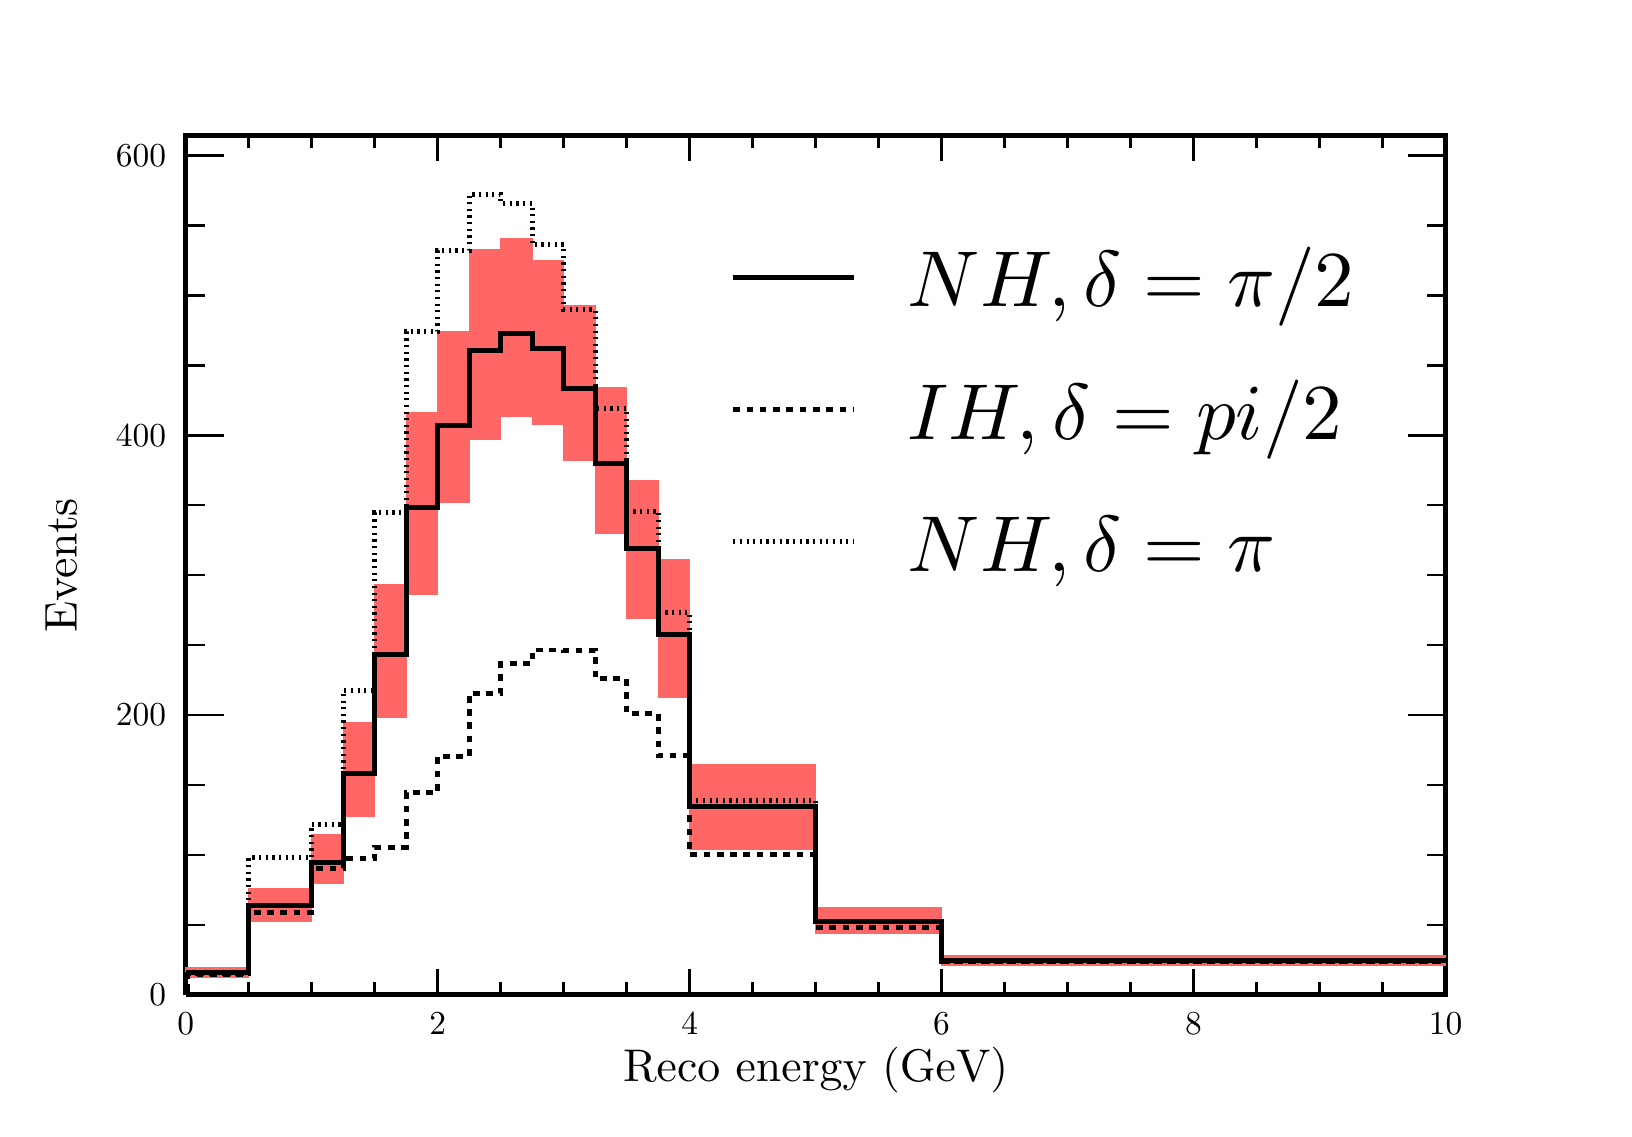
\begin{tikzpicture}
\pgfdeclareplotmark{cross} {
\pgfpathmoveto{\pgfpoint{-0.3\pgfplotmarksize}{\pgfplotmarksize}}
\pgfpathlineto{\pgfpoint{+0.3\pgfplotmarksize}{\pgfplotmarksize}}
\pgfpathlineto{\pgfpoint{+0.3\pgfplotmarksize}{0.3\pgfplotmarksize}}
\pgfpathlineto{\pgfpoint{+1\pgfplotmarksize}{0.3\pgfplotmarksize}}
\pgfpathlineto{\pgfpoint{+1\pgfplotmarksize}{-0.3\pgfplotmarksize}}
\pgfpathlineto{\pgfpoint{+0.3\pgfplotmarksize}{-0.3\pgfplotmarksize}}
\pgfpathlineto{\pgfpoint{+0.3\pgfplotmarksize}{-1.\pgfplotmarksize}}
\pgfpathlineto{\pgfpoint{-0.3\pgfplotmarksize}{-1.\pgfplotmarksize}}
\pgfpathlineto{\pgfpoint{-0.3\pgfplotmarksize}{-0.3\pgfplotmarksize}}
\pgfpathlineto{\pgfpoint{-1.\pgfplotmarksize}{-0.3\pgfplotmarksize}}
\pgfpathlineto{\pgfpoint{-1.\pgfplotmarksize}{0.3\pgfplotmarksize}}
\pgfpathlineto{\pgfpoint{-0.3\pgfplotmarksize}{0.3\pgfplotmarksize}}
\pgfpathclose
\pgfusepathqstroke
}
\pgfdeclareplotmark{cross*} {
\pgfpathmoveto{\pgfpoint{-0.3\pgfplotmarksize}{\pgfplotmarksize}}
\pgfpathlineto{\pgfpoint{+0.3\pgfplotmarksize}{\pgfplotmarksize}}
\pgfpathlineto{\pgfpoint{+0.3\pgfplotmarksize}{0.3\pgfplotmarksize}}
\pgfpathlineto{\pgfpoint{+1\pgfplotmarksize}{0.3\pgfplotmarksize}}
\pgfpathlineto{\pgfpoint{+1\pgfplotmarksize}{-0.3\pgfplotmarksize}}
\pgfpathlineto{\pgfpoint{+0.3\pgfplotmarksize}{-0.3\pgfplotmarksize}}
\pgfpathlineto{\pgfpoint{+0.3\pgfplotmarksize}{-1.\pgfplotmarksize}}
\pgfpathlineto{\pgfpoint{-0.3\pgfplotmarksize}{-1.\pgfplotmarksize}}
\pgfpathlineto{\pgfpoint{-0.3\pgfplotmarksize}{-0.3\pgfplotmarksize}}
\pgfpathlineto{\pgfpoint{-1.\pgfplotmarksize}{-0.3\pgfplotmarksize}}
\pgfpathlineto{\pgfpoint{-1.\pgfplotmarksize}{0.3\pgfplotmarksize}}
\pgfpathlineto{\pgfpoint{-0.3\pgfplotmarksize}{0.3\pgfplotmarksize}}
\pgfpathclose
\pgfusepathqfillstroke
}
\pgfdeclareplotmark{newstar} {
\pgfpathmoveto{\pgfqpoint{0pt}{\pgfplotmarksize}}
\pgfpathlineto{\pgfqpointpolar{44}{0.5\pgfplotmarksize}}
\pgfpathlineto{\pgfqpointpolar{18}{\pgfplotmarksize}}
\pgfpathlineto{\pgfqpointpolar{-20}{0.5\pgfplotmarksize}}
\pgfpathlineto{\pgfqpointpolar{-54}{\pgfplotmarksize}}
\pgfpathlineto{\pgfqpointpolar{-90}{0.5\pgfplotmarksize}}
\pgfpathlineto{\pgfqpointpolar{234}{\pgfplotmarksize}}
\pgfpathlineto{\pgfqpointpolar{198}{0.5\pgfplotmarksize}}
\pgfpathlineto{\pgfqpointpolar{162}{\pgfplotmarksize}}
\pgfpathlineto{\pgfqpointpolar{134}{0.5\pgfplotmarksize}}
\pgfpathclose
\pgfusepathqstroke
}
\pgfdeclareplotmark{newstar*} {
\pgfpathmoveto{\pgfqpoint{0pt}{\pgfplotmarksize}}
\pgfpathlineto{\pgfqpointpolar{44}{0.5\pgfplotmarksize}}
\pgfpathlineto{\pgfqpointpolar{18}{\pgfplotmarksize}}
\pgfpathlineto{\pgfqpointpolar{-20}{0.5\pgfplotmarksize}}
\pgfpathlineto{\pgfqpointpolar{-54}{\pgfplotmarksize}}
\pgfpathlineto{\pgfqpointpolar{-90}{0.5\pgfplotmarksize}}
\pgfpathlineto{\pgfqpointpolar{234}{\pgfplotmarksize}}
\pgfpathlineto{\pgfqpointpolar{198}{0.5\pgfplotmarksize}}
\pgfpathlineto{\pgfqpointpolar{162}{\pgfplotmarksize}}
\pgfpathlineto{\pgfqpointpolar{134}{0.5\pgfplotmarksize}}
\pgfpathclose
\pgfusepathqfillstroke
}
\definecolor{c}{rgb}{0.999,0.999,0.999};
\draw [color=c, fill=c] (0,0) rectangle (20,13.639);
\draw [color=c, fill=c] (2,1.3639) rectangle (18,12.2751);
\definecolor{c}{rgb}{0,0,0};
\draw [c,line width=1.8] (2,1.3639) -- (2,12.2751) -- (18,12.2751) -- (18,1.3639) -- (2,1.3639);
\definecolor{c}{rgb}{0.999,0.999,0.999};
\draw [color=c, fill=c] (2,1.3639) rectangle (18,12.2751);
\definecolor{c}{rgb}{0,0,0};
\draw [c,line width=1.8] (2,1.3639) -- (2,12.2751) -- (18,12.2751) -- (18,1.3639) -- (2,1.3639);
\draw [c,line width=1.8] (2,1.64385) -- (2.8,1.64385) -- (2.8,2.4955) -- (3.6,2.4955) -- (3.6,3.04067) -- (4,3.04067) -- (4,4.17002) -- (4.4,4.17002) -- (4.4,5.68074) -- (4.8,5.68074) -- (4.8,7.55117) -- (5.2,7.55117) -- (5.2,8.59541) --
 (5.6,8.59541) -- (5.6,9.54186) -- (6,9.54186) -- (6,9.75711) -- (6.4,9.75711) -- (6.4,9.57209) -- (6.8,9.57209) -- (6.8,9.0685) -- (7.2,9.0685) -- (7.2,8.10527) -- (7.6,8.10527) -- (7.6,7.03512) -- (8,7.03512) -- (8,5.93304) -- (8.4,5.93304) --
 (8.4,3.75508) -- (10,3.75508) -- (10,2.29637) -- (11.6,2.29637) -- (11.6,1.79751) -- (18,1.79751);
\draw [c,line width=0.9] (2,1.3639) -- (18,1.3639);
\draw [c,line width=0.9] (2,1.69123) -- (2,1.3639);
\draw [c,line width=0.9] (2.8,1.52756) -- (2.8,1.3639);
\draw [c,line width=0.9] (3.6,1.52756) -- (3.6,1.3639);
\draw [c,line width=0.9] (4.4,1.52756) -- (4.4,1.3639);
\draw [c,line width=0.9] (5.2,1.69123) -- (5.2,1.3639);
\draw [c,line width=0.9] (6,1.52756) -- (6,1.3639);
\draw [c,line width=0.9] (6.8,1.52756) -- (6.8,1.3639);
\draw [c,line width=0.9] (7.6,1.52756) -- (7.6,1.3639);
\draw [c,line width=0.9] (8.4,1.69123) -- (8.4,1.3639);
\draw [c,line width=0.9] (9.2,1.52756) -- (9.2,1.3639);
\draw [c,line width=0.9] (10,1.52756) -- (10,1.3639);
\draw [c,line width=0.9] (10.8,1.52756) -- (10.8,1.3639);
\draw [c,line width=0.9] (11.6,1.69123) -- (11.6,1.3639);
\draw [c,line width=0.9] (12.4,1.52756) -- (12.4,1.3639);
\draw [c,line width=0.9] (13.2,1.52756) -- (13.2,1.3639);
\draw [c,line width=0.9] (14,1.52756) -- (14,1.3639);
\draw [c,line width=0.9] (14.8,1.69123) -- (14.8,1.3639);
\draw [c,line width=0.9] (15.6,1.52756) -- (15.6,1.3639);
\draw [c,line width=0.9] (16.4,1.52756) -- (16.4,1.3639);
\draw [c,line width=0.9] (17.2,1.52756) -- (17.2,1.3639);
\draw [c,line width=0.9] (18,1.69123) -- (18,1.3639);
\draw [anchor=base] (2,0.859255) node[scale=1.20912, color=c, rotate=0]{0};
\draw [anchor=base] (5.2,0.859255) node[scale=1.20912, color=c, rotate=0]{2};
\draw [anchor=base] (8.4,0.859255) node[scale=1.20912, color=c, rotate=0]{4};
\draw [anchor=base] (11.6,0.859255) node[scale=1.20912, color=c, rotate=0]{6};
\draw [anchor=base] (14.8,0.859255) node[scale=1.20912, color=c, rotate=0]{8};
\draw [anchor=base] (18,0.859255) node[scale=1.20912, color=c, rotate=0]{10};
\draw (10,0.403714) node[scale=1.65459, color=c, rotate=0]{Reco energy (GeV)};
\draw [c,line width=0.9] (2,12.2751) -- (18,12.2751);
\draw [c,line width=0.9] (2,11.9477) -- (2,12.2751);
\draw [c,line width=0.9] (2.8,12.1114) -- (2.8,12.2751);
\draw [c,line width=0.9] (3.6,12.1114) -- (3.6,12.2751);
\draw [c,line width=0.9] (4.4,12.1114) -- (4.4,12.2751);
\draw [c,line width=0.9] (5.2,11.9477) -- (5.2,12.2751);
\draw [c,line width=0.9] (6,12.1114) -- (6,12.2751);
\draw [c,line width=0.9] (6.8,12.1114) -- (6.8,12.2751);
\draw [c,line width=0.9] (7.6,12.1114) -- (7.6,12.2751);
\draw [c,line width=0.9] (8.4,11.9477) -- (8.4,12.2751);
\draw [c,line width=0.9] (9.2,12.1114) -- (9.2,12.2751);
\draw [c,line width=0.9] (10,12.1114) -- (10,12.2751);
\draw [c,line width=0.9] (10.8,12.1114) -- (10.8,12.2751);
\draw [c,line width=0.9] (11.6,11.9477) -- (11.6,12.2751);
\draw [c,line width=0.9] (12.4,12.1114) -- (12.4,12.2751);
\draw [c,line width=0.9] (13.2,12.1114) -- (13.2,12.2751);
\draw [c,line width=0.9] (14,12.1114) -- (14,12.2751);
\draw [c,line width=0.9] (14.8,11.9477) -- (14.8,12.2751);
\draw [c,line width=0.9] (15.6,12.1114) -- (15.6,12.2751);
\draw [c,line width=0.9] (16.4,12.1114) -- (16.4,12.2751);
\draw [c,line width=0.9] (17.2,12.1114) -- (17.2,12.2751);
\draw [c,line width=0.9] (18,11.9477) -- (18,12.2751);
\draw [c,line width=0.9] (2,1.3639) -- (2,12.2751);
\draw [c,line width=0.9] (2.48,1.3639) -- (2,1.3639);
\draw [c,line width=0.9] (2.24,2.25207) -- (2,2.25207);
\draw [c,line width=0.9] (2.24,3.14024) -- (2,3.14024);
\draw [c,line width=0.9] (2.24,4.02841) -- (2,4.02841);
\draw [c,line width=0.9] (2.48,4.91657) -- (2,4.91657);
\draw [c,line width=0.9] (2.24,5.80474) -- (2,5.80474);
\draw [c,line width=0.9] (2.24,6.69291) -- (2,6.69291);
\draw [c,line width=0.9] (2.24,7.58108) -- (2,7.58108);
\draw [c,line width=0.9] (2.48,8.46925) -- (2,8.46925);
\draw [c,line width=0.9] (2.24,9.35742) -- (2,9.35742);
\draw [c,line width=0.9] (2.24,10.2456) -- (2,10.2456);
\draw [c,line width=0.9] (2.24,11.1338) -- (2,11.1338);
\draw [c,line width=0.9] (2.48,12.0219) -- (2,12.0219);
\draw [c,line width=0.9] (2.48,12.0219) -- (2,12.0219);
\draw [anchor= east] (1.9,1.3639) node[scale=1.20912, color=c, rotate=0]{0};
\draw [anchor= east] (1.9,4.91657) node[scale=1.20912, color=c, rotate=0]{200};
\draw [anchor= east] (1.9,8.46925) node[scale=1.20912, color=c, rotate=0]{400};
\draw [anchor= east] (1.9,12.0219) node[scale=1.20912, color=c, rotate=0]{600};
\draw (0.416,6.81948) node[scale=1.65459, color=c, rotate=90]{Events};
\draw [c,line width=0.9] (18,1.3639) -- (18,12.2751);
\draw [c,line width=0.9] (17.52,1.3639) -- (18,1.3639);
\draw [c,line width=0.9] (17.76,2.25207) -- (18,2.25207);
\draw [c,line width=0.9] (17.76,3.14024) -- (18,3.14024);
\draw [c,line width=0.9] (17.76,4.02841) -- (18,4.02841);
\draw [c,line width=0.9] (17.52,4.91657) -- (18,4.91657);
\draw [c,line width=0.9] (17.76,5.80474) -- (18,5.80474);
\draw [c,line width=0.9] (17.76,6.69291) -- (18,6.69291);
\draw [c,line width=0.9] (17.76,7.58108) -- (18,7.58108);
\draw [c,line width=0.9] (17.52,8.46925) -- (18,8.46925);
\draw [c,line width=0.9] (17.76,9.35742) -- (18,9.35742);
\draw [c,line width=0.9] (17.76,10.2456) -- (18,10.2456);
\draw [c,line width=0.9] (17.76,11.1338) -- (18,11.1338);
\draw [c,line width=0.9] (17.52,12.0219) -- (18,12.0219);
\draw [c,line width=0.9] (17.52,12.0219) -- (18,12.0219);
\definecolor{c}{rgb}{1,0.4,0.4};
\draw [color=c, fill=c] (2,1.58015) rectangle (2.8,1.7134);
\draw [color=c, fill=c] (2.8,2.29213) rectangle (3.6,2.71872);
\draw [color=c, fill=c] (3.6,2.78395) rectangle (4,3.39413);
\draw [color=c, fill=c] (4,3.62681) rectangle (4.4,4.82152);
\draw [color=c, fill=c] (4.4,4.88881) rectangle (4.8,6.57058);
\draw [color=c, fill=c] (4.8,6.44707) rectangle (5.2,8.76228);
\draw [color=c, fill=c] (5.2,7.61558) rectangle (5.6,9.7925);
\draw [color=c, fill=c] (5.6,8.41168) rectangle (6,10.8229);
\draw [color=c, fill=c] (6,8.70899) rectangle (6.4,10.9686);
\draw [color=c, fill=c] (6.4,8.60219) rectangle (6.8,10.6924);
\draw [color=c, fill=c] (6.8,8.15486) rectangle (7.2,10.1205);
\draw [color=c, fill=c] (7.2,7.21737) rectangle (7.6,9.06911);
\draw [color=c, fill=c] (7.6,6.1376) rectangle (8,7.89091);
\draw [color=c, fill=c] (8,5.13712) rectangle (8.4,6.88859);
\draw [color=c, fill=c] (8.4,3.20749) rectangle (10,4.28877);
\draw [color=c, fill=c] (10,2.14873) rectangle (11.6,2.46598);
\draw [color=c, fill=c] (11.6,1.73357) rectangle (18,1.86509);
\definecolor{c}{rgb}{0,0,0};
\draw [c,line width=1.8] (2,1.64385) -- (2.8,1.64385) -- (2.8,2.4955) -- (3.6,2.4955) -- (3.6,3.04067) -- (4,3.04067) -- (4,4.17002) -- (4.4,4.17002) -- (4.4,5.68074) -- (4.8,5.68074) -- (4.8,7.55117) -- (5.2,7.55117) -- (5.2,8.59541) --
 (5.6,8.59541) -- (5.6,9.54186) -- (6,9.54186) -- (6,9.75711) -- (6.4,9.75711) -- (6.4,9.57209) -- (6.8,9.57209) -- (6.8,9.0685) -- (7.2,9.0685) -- (7.2,8.10527) -- (7.6,8.10527) -- (7.6,7.03512) -- (8,7.03512) -- (8,5.93304) -- (8.4,5.93304) --
 (8.4,3.75508) -- (10,3.75508) -- (10,2.29637) -- (11.6,2.29637) -- (11.6,1.79751) -- (18,1.79751);
\draw [c,dash pattern=on 2.40pt off 2.40pt ,line width=1.8] (2.02865,1.39255) -- (2.02865,1.61977) -- (2.8,1.61977) -- (2.8,2.41107) -- (3.6,2.41107) -- (3.6,2.96834) -- (4,2.96834) -- (4,3.09236) -- (4.4,3.09236) -- (4.4,3.23892) -- (4.8,3.23892) --
 (4.8,3.933) -- (5.2,3.933) -- (5.2,4.396) -- (5.6,4.396) -- (5.6,5.1953) -- (6,5.1953) -- (6,5.56987) -- (6.4,5.56987) -- (6.4,5.74248) -- (6.8,5.74248) -- (6.8,5.73905) -- (7.2,5.73905) -- (7.2,5.37435) -- (7.6,5.37435) -- (7.6,4.93637) --
 (8,4.93637) -- (8,4.39961) -- (8.4,4.39961) -- (8.4,3.14541) -- (10,3.14541) -- (10,2.21288) -- (11.6,2.21288) -- (11.6,1.78649) -- (18,1.78649);
\draw [c,dash pattern=on 0.80pt off 1.60pt ,line width=1.8] (2.02865,1.39255) -- (2.02865,1.63661) -- (2.8,1.63661) -- (2.8,3.10507) -- (3.6,3.10507) -- (3.6,3.53228) -- (4,3.53228) -- (4,5.22798) -- (4.4,5.22798) -- (4.4,7.48346) -- (4.8,7.48346) --
 (4.8,9.78237) -- (5.2,9.78237) -- (5.2,10.8173) -- (5.6,10.8173) -- (5.6,11.5299) -- (6,11.5299) -- (6,11.4147) -- (6.4,11.4147) -- (6.4,10.8885) -- (6.8,10.8885) -- (6.8,10.0652) -- (7.2,10.0652) -- (7.2,8.81124) -- (7.6,8.81124) -- (7.6,7.50156)
 -- (8,7.50156) -- (8,6.22071) -- (8.4,6.22071) -- (8.4,3.82997) -- (10,3.82997) -- (10,2.29002) -- (11.6,2.29002) -- (11.6,1.79186) -- (18,1.79186);
\definecolor{c}{rgb}{1,1,1};
\draw [color=c, fill=c] (8.62464,6.27507) rectangle (17.3925,11.3181);
\definecolor{c}{rgb}{0,0,0};
\draw [anchor=base west] (10.8166,10.0993) node[scale=2.86371, color=c, rotate=0]{$NH, \delta = \pi/2$};
\draw [c,line width=1.8] (8.95344,10.4776) -- (10.4878,10.4776);
\draw [anchor=base west] (10.8166,8.41834) node[scale=2.86371, color=c, rotate=0]{$IH, \delta = pi/2$};
\draw [c,dash pattern=on 2.40pt off 2.40pt ,line width=1.8] (8.95344,8.79656) -- (10.4878,8.79656);
\draw [anchor=base west] (10.8166,6.73734) node[scale=2.86371, color=c, rotate=0]{$NH, \delta = \pi$};
\draw [c,dash pattern=on 0.80pt off 1.60pt ,line width=1.8] (8.95344,7.11557) -- (10.4878,7.11557);
\end{tikzpicture}

		\end{adjustbox}
	\end{minipage}
	\hfill
	\begin{minipage}[t]{.5\linewidth}
		\begin{adjustbox}{max totalsize=\linewidth, center}
			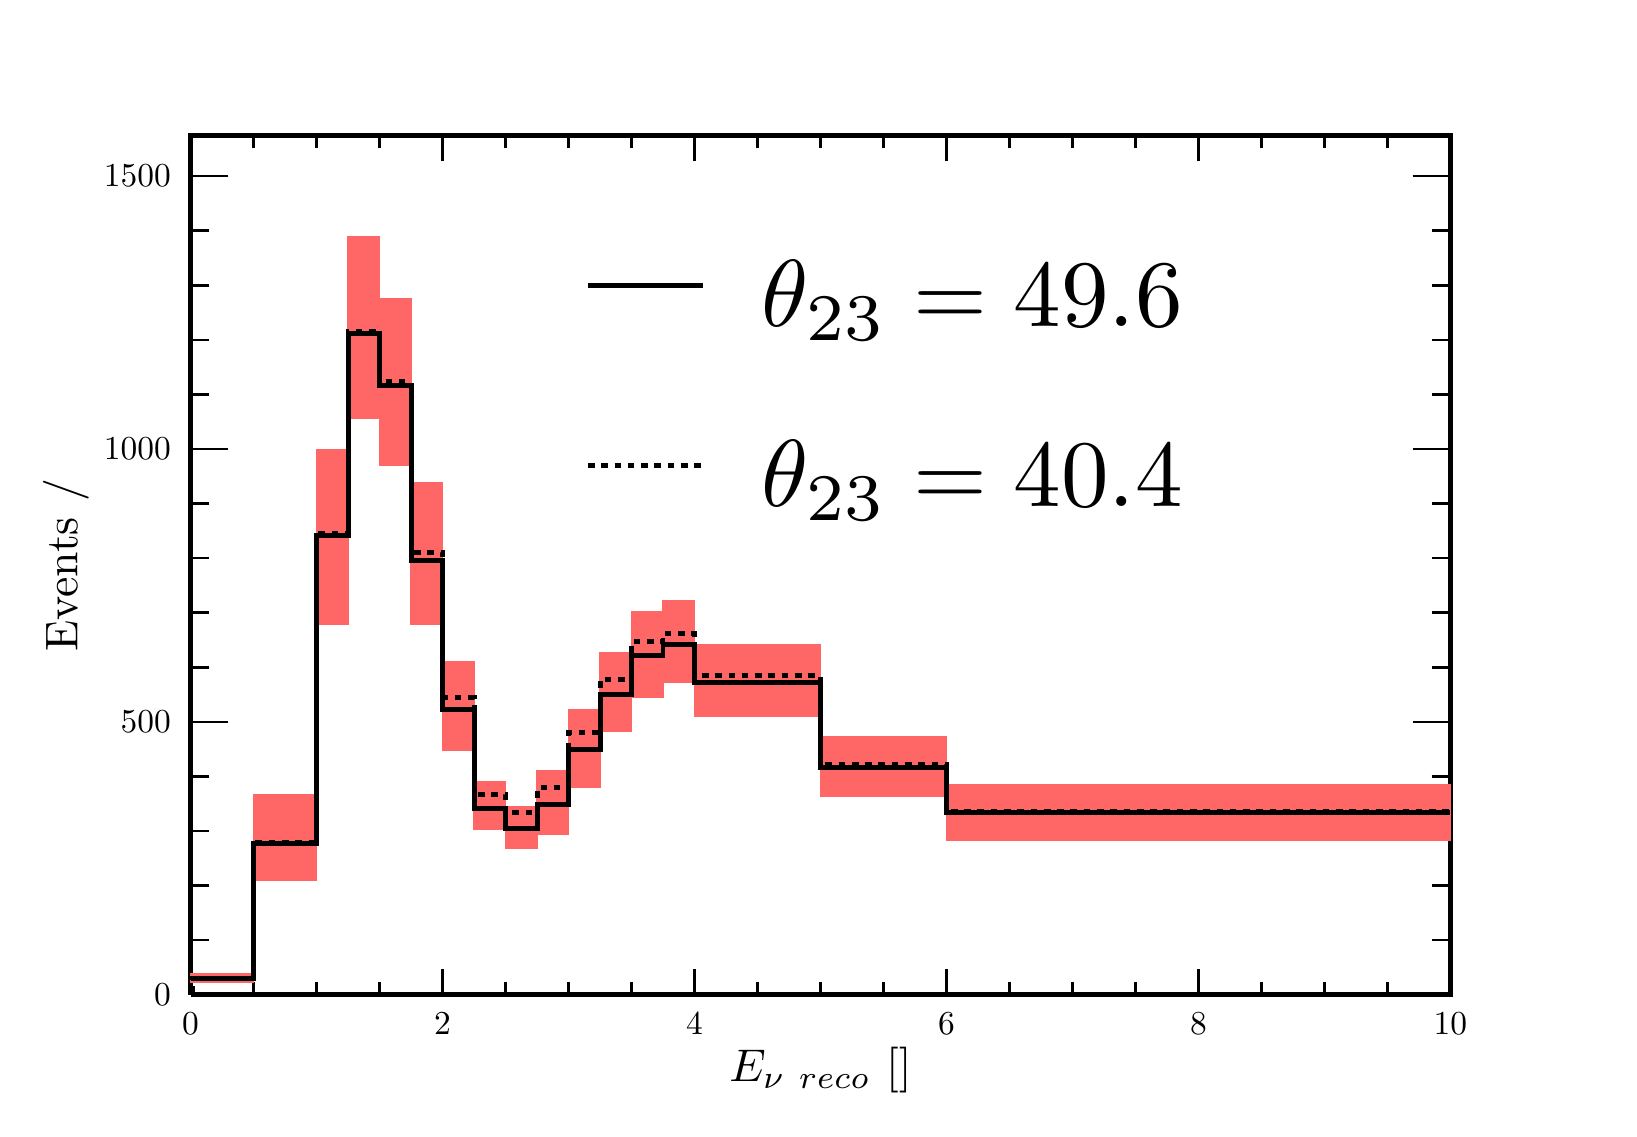
\begin{tikzpicture}
\pgfdeclareplotmark{cross} {
\pgfpathmoveto{\pgfpoint{-0.3\pgfplotmarksize}{\pgfplotmarksize}}
\pgfpathlineto{\pgfpoint{+0.3\pgfplotmarksize}{\pgfplotmarksize}}
\pgfpathlineto{\pgfpoint{+0.3\pgfplotmarksize}{0.3\pgfplotmarksize}}
\pgfpathlineto{\pgfpoint{+1\pgfplotmarksize}{0.3\pgfplotmarksize}}
\pgfpathlineto{\pgfpoint{+1\pgfplotmarksize}{-0.3\pgfplotmarksize}}
\pgfpathlineto{\pgfpoint{+0.3\pgfplotmarksize}{-0.3\pgfplotmarksize}}
\pgfpathlineto{\pgfpoint{+0.3\pgfplotmarksize}{-1.\pgfplotmarksize}}
\pgfpathlineto{\pgfpoint{-0.3\pgfplotmarksize}{-1.\pgfplotmarksize}}
\pgfpathlineto{\pgfpoint{-0.3\pgfplotmarksize}{-0.3\pgfplotmarksize}}
\pgfpathlineto{\pgfpoint{-1.\pgfplotmarksize}{-0.3\pgfplotmarksize}}
\pgfpathlineto{\pgfpoint{-1.\pgfplotmarksize}{0.3\pgfplotmarksize}}
\pgfpathlineto{\pgfpoint{-0.3\pgfplotmarksize}{0.3\pgfplotmarksize}}
\pgfpathclose
\pgfusepathqstroke
}
\pgfdeclareplotmark{cross*} {
\pgfpathmoveto{\pgfpoint{-0.3\pgfplotmarksize}{\pgfplotmarksize}}
\pgfpathlineto{\pgfpoint{+0.3\pgfplotmarksize}{\pgfplotmarksize}}
\pgfpathlineto{\pgfpoint{+0.3\pgfplotmarksize}{0.3\pgfplotmarksize}}
\pgfpathlineto{\pgfpoint{+1\pgfplotmarksize}{0.3\pgfplotmarksize}}
\pgfpathlineto{\pgfpoint{+1\pgfplotmarksize}{-0.3\pgfplotmarksize}}
\pgfpathlineto{\pgfpoint{+0.3\pgfplotmarksize}{-0.3\pgfplotmarksize}}
\pgfpathlineto{\pgfpoint{+0.3\pgfplotmarksize}{-1.\pgfplotmarksize}}
\pgfpathlineto{\pgfpoint{-0.3\pgfplotmarksize}{-1.\pgfplotmarksize}}
\pgfpathlineto{\pgfpoint{-0.3\pgfplotmarksize}{-0.3\pgfplotmarksize}}
\pgfpathlineto{\pgfpoint{-1.\pgfplotmarksize}{-0.3\pgfplotmarksize}}
\pgfpathlineto{\pgfpoint{-1.\pgfplotmarksize}{0.3\pgfplotmarksize}}
\pgfpathlineto{\pgfpoint{-0.3\pgfplotmarksize}{0.3\pgfplotmarksize}}
\pgfpathclose
\pgfusepathqfillstroke
}
\pgfdeclareplotmark{newstar} {
\pgfpathmoveto{\pgfqpoint{0pt}{\pgfplotmarksize}}
\pgfpathlineto{\pgfqpointpolar{44}{0.5\pgfplotmarksize}}
\pgfpathlineto{\pgfqpointpolar{18}{\pgfplotmarksize}}
\pgfpathlineto{\pgfqpointpolar{-20}{0.5\pgfplotmarksize}}
\pgfpathlineto{\pgfqpointpolar{-54}{\pgfplotmarksize}}
\pgfpathlineto{\pgfqpointpolar{-90}{0.5\pgfplotmarksize}}
\pgfpathlineto{\pgfqpointpolar{234}{\pgfplotmarksize}}
\pgfpathlineto{\pgfqpointpolar{198}{0.5\pgfplotmarksize}}
\pgfpathlineto{\pgfqpointpolar{162}{\pgfplotmarksize}}
\pgfpathlineto{\pgfqpointpolar{134}{0.5\pgfplotmarksize}}
\pgfpathclose
\pgfusepathqstroke
}
\pgfdeclareplotmark{newstar*} {
\pgfpathmoveto{\pgfqpoint{0pt}{\pgfplotmarksize}}
\pgfpathlineto{\pgfqpointpolar{44}{0.5\pgfplotmarksize}}
\pgfpathlineto{\pgfqpointpolar{18}{\pgfplotmarksize}}
\pgfpathlineto{\pgfqpointpolar{-20}{0.5\pgfplotmarksize}}
\pgfpathlineto{\pgfqpointpolar{-54}{\pgfplotmarksize}}
\pgfpathlineto{\pgfqpointpolar{-90}{0.5\pgfplotmarksize}}
\pgfpathlineto{\pgfqpointpolar{234}{\pgfplotmarksize}}
\pgfpathlineto{\pgfqpointpolar{198}{0.5\pgfplotmarksize}}
\pgfpathlineto{\pgfqpointpolar{162}{\pgfplotmarksize}}
\pgfpathlineto{\pgfqpointpolar{134}{0.5\pgfplotmarksize}}
\pgfpathclose
\pgfusepathqfillstroke
}
\definecolor{c}{rgb}{0.999,0.999,0.999};
\draw [color=c, fill=c] (0,0) rectangle (20,13.639);
\draw [color=c, fill=c] (2,1.3639) rectangle (18,12.2751);
\definecolor{c}{rgb}{0,0,0};
\draw [c,line width=1.8] (2,1.3639) -- (2,12.2751) -- (18,12.2751) -- (18,1.3639) -- (2,1.3639);
\definecolor{c}{rgb}{0.999,0.999,0.999};
\draw [color=c, fill=c] (2,1.3639) rectangle (18,12.2751);
\definecolor{c}{rgb}{0,0,0};
\draw [c,line width=1.8] (2,1.3639) -- (2,12.2751) -- (18,12.2751) -- (18,1.3639) -- (2,1.3639);
\draw [c,line width=1.8] (2,1.57169) -- (2.8,1.57169) -- (2.8,3.28175) -- (3.6,3.28175) -- (3.6,7.19234) -- (4,7.19234) -- (4,9.75711) -- (4.4,9.75711) -- (4.4,9.09746) -- (4.8,9.09746) -- (4.8,6.88525) -- (5.2,6.88525) -- (5.2,4.99266) --
 (5.6,4.99266) -- (5.6,3.73479) -- (6,3.73479) -- (6,3.47247) -- (6.4,3.47247) -- (6.4,3.78133) -- (6.8,3.78133) -- (6.8,4.48314) -- (7.2,4.48314) -- (7.2,5.17879) -- (7.6,5.17879) -- (7.6,5.67814) -- (8,5.67814) -- (8,5.81819) -- (8.4,5.81819) --
 (8.4,5.33518) -- (10,5.33518) -- (10,4.25465) -- (11.6,4.25465) -- (11.6,3.67823) -- (18,3.67823);
\draw [c,line width=0.9] (2,1.3639) -- (18,1.3639);
\draw [c,line width=0.9] (2,1.69123) -- (2,1.3639);
\draw [c,line width=0.9] (2.8,1.52756) -- (2.8,1.3639);
\draw [c,line width=0.9] (3.6,1.52756) -- (3.6,1.3639);
\draw [c,line width=0.9] (4.4,1.52756) -- (4.4,1.3639);
\draw [c,line width=0.9] (5.2,1.69123) -- (5.2,1.3639);
\draw [c,line width=0.9] (6,1.52756) -- (6,1.3639);
\draw [c,line width=0.9] (6.8,1.52756) -- (6.8,1.3639);
\draw [c,line width=0.9] (7.6,1.52756) -- (7.6,1.3639);
\draw [c,line width=0.9] (8.4,1.69123) -- (8.4,1.3639);
\draw [c,line width=0.9] (9.2,1.52756) -- (9.2,1.3639);
\draw [c,line width=0.9] (10,1.52756) -- (10,1.3639);
\draw [c,line width=0.9] (10.8,1.52756) -- (10.8,1.3639);
\draw [c,line width=0.9] (11.6,1.69123) -- (11.6,1.3639);
\draw [c,line width=0.9] (12.4,1.52756) -- (12.4,1.3639);
\draw [c,line width=0.9] (13.2,1.52756) -- (13.2,1.3639);
\draw [c,line width=0.9] (14,1.52756) -- (14,1.3639);
\draw [c,line width=0.9] (14.8,1.69123) -- (14.8,1.3639);
\draw [c,line width=0.9] (15.6,1.52756) -- (15.6,1.3639);
\draw [c,line width=0.9] (16.4,1.52756) -- (16.4,1.3639);
\draw [c,line width=0.9] (17.2,1.52756) -- (17.2,1.3639);
\draw [c,line width=0.9] (18,1.69123) -- (18,1.3639);
\draw [anchor=base] (2,0.859255) node[scale=1.20912, color=c, rotate=0]{0};
\draw [anchor=base] (5.2,0.859255) node[scale=1.20912, color=c, rotate=0]{2};
\draw [anchor=base] (8.4,0.859255) node[scale=1.20912, color=c, rotate=0]{4};
\draw [anchor=base] (11.6,0.859255) node[scale=1.20912, color=c, rotate=0]{6};
\draw [anchor=base] (14.8,0.859255) node[scale=1.20912, color=c, rotate=0]{8};
\draw [anchor=base] (18,0.859255) node[scale=1.20912, color=c, rotate=0]{10};
\draw (10,0.403714) node[scale=1.65459, color=c, rotate=0]{$E_{\nu~\text{reco}}$ [\si{\GeV}]};
\draw [c,line width=0.9] (2,12.2751) -- (18,12.2751);
\draw [c,line width=0.9] (2,11.9477) -- (2,12.2751);
\draw [c,line width=0.9] (2.8,12.1114) -- (2.8,12.2751);
\draw [c,line width=0.9] (3.6,12.1114) -- (3.6,12.2751);
\draw [c,line width=0.9] (4.4,12.1114) -- (4.4,12.2751);
\draw [c,line width=0.9] (5.2,11.9477) -- (5.2,12.2751);
\draw [c,line width=0.9] (6,12.1114) -- (6,12.2751);
\draw [c,line width=0.9] (6.8,12.1114) -- (6.8,12.2751);
\draw [c,line width=0.9] (7.6,12.1114) -- (7.6,12.2751);
\draw [c,line width=0.9] (8.4,11.9477) -- (8.4,12.2751);
\draw [c,line width=0.9] (9.2,12.1114) -- (9.2,12.2751);
\draw [c,line width=0.9] (10,12.1114) -- (10,12.2751);
\draw [c,line width=0.9] (10.8,12.1114) -- (10.8,12.2751);
\draw [c,line width=0.9] (11.6,11.9477) -- (11.6,12.2751);
\draw [c,line width=0.9] (12.4,12.1114) -- (12.4,12.2751);
\draw [c,line width=0.9] (13.2,12.1114) -- (13.2,12.2751);
\draw [c,line width=0.9] (14,12.1114) -- (14,12.2751);
\draw [c,line width=0.9] (14.8,11.9477) -- (14.8,12.2751);
\draw [c,line width=0.9] (15.6,12.1114) -- (15.6,12.2751);
\draw [c,line width=0.9] (16.4,12.1114) -- (16.4,12.2751);
\draw [c,line width=0.9] (17.2,12.1114) -- (17.2,12.2751);
\draw [c,line width=0.9] (18,11.9477) -- (18,12.2751);
\draw [c,line width=0.9] (2,1.3639) -- (2,12.2751);
\draw [c,line width=0.9] (2.48,1.3639) -- (2,1.3639);
\draw [c,line width=0.9] (2.24,2.05703) -- (2,2.05703);
\draw [c,line width=0.9] (2.24,2.75017) -- (2,2.75017);
\draw [c,line width=0.9] (2.24,3.4433) -- (2,3.4433);
\draw [c,line width=0.9] (2.24,4.13643) -- (2,4.13643);
\draw [c,line width=0.9] (2.48,4.82957) -- (2,4.82957);
\draw [c,line width=0.9] (2.24,5.5227) -- (2,5.5227);
\draw [c,line width=0.9] (2.24,6.21584) -- (2,6.21584);
\draw [c,line width=0.9] (2.24,6.90897) -- (2,6.90897);
\draw [c,line width=0.9] (2.24,7.60211) -- (2,7.60211);
\draw [c,line width=0.9] (2.48,8.29524) -- (2,8.29524);
\draw [c,line width=0.9] (2.24,8.98838) -- (2,8.98838);
\draw [c,line width=0.9] (2.24,9.68151) -- (2,9.68151);
\draw [c,line width=0.9] (2.24,10.3746) -- (2,10.3746);
\draw [c,line width=0.9] (2.24,11.0678) -- (2,11.0678);
\draw [c,line width=0.9] (2.48,11.7609) -- (2,11.7609);
\draw [c,line width=0.9] (2.48,11.7609) -- (2,11.7609);
\draw [anchor= east] (1.9,1.3639) node[scale=1.20912, color=c, rotate=0]{0};
\draw [anchor= east] (1.9,4.82957) node[scale=1.20912, color=c, rotate=0]{500};
\draw [anchor= east] (1.9,8.29524) node[scale=1.20912, color=c, rotate=0]{1000};
\draw [anchor= east] (1.9,11.7609) node[scale=1.20912, color=c, rotate=0]{1500};
\draw (0.416,6.81948) node[scale=1.65459, color=c, rotate=90]{Events / \si{\GeV}};
\draw [c,line width=0.9] (18,1.3639) -- (18,12.2751);
\draw [c,line width=0.9] (17.52,1.3639) -- (18,1.3639);
\draw [c,line width=0.9] (17.76,2.05703) -- (18,2.05703);
\draw [c,line width=0.9] (17.76,2.75017) -- (18,2.75017);
\draw [c,line width=0.9] (17.76,3.4433) -- (18,3.4433);
\draw [c,line width=0.9] (17.76,4.13643) -- (18,4.13643);
\draw [c,line width=0.9] (17.52,4.82957) -- (18,4.82957);
\draw [c,line width=0.9] (17.76,5.5227) -- (18,5.5227);
\draw [c,line width=0.9] (17.76,6.21584) -- (18,6.21584);
\draw [c,line width=0.9] (17.76,6.90897) -- (18,6.90897);
\draw [c,line width=0.9] (17.76,7.60211) -- (18,7.60211);
\draw [c,line width=0.9] (17.52,8.29524) -- (18,8.29524);
\draw [c,line width=0.9] (17.76,8.98838) -- (18,8.98838);
\draw [c,line width=0.9] (17.76,9.68151) -- (18,9.68151);
\draw [c,line width=0.9] (17.76,10.3746) -- (18,10.3746);
\draw [c,line width=0.9] (17.76,11.0678) -- (18,11.0678);
\draw [c,line width=0.9] (17.52,11.7609) -- (18,11.7609);
\draw [c,line width=0.9] (17.52,11.7609) -- (18,11.7609);
\definecolor{c}{rgb}{1,0.4,0.4};
\draw [color=c, fill=c] (2,1.52109) rectangle (2.8,1.63215);
\draw [color=c, fill=c] (2.8,2.80955) rectangle (3.6,3.90192);
\draw [color=c, fill=c] (3.6,6.06063) rectangle (4,8.2942);
\draw [color=c, fill=c] (4,8.6774) rectangle (4.4,10.9896);
\draw [color=c, fill=c] (4.4,8.08761) rectangle (4.8,10.2035);
\draw [color=c, fill=c] (4.8,6.06386) rectangle (5.2,7.86839);
\draw [color=c, fill=c] (5.2,4.46483) rectangle (5.6,5.58935);
\draw [color=c, fill=c] (5.6,3.46701) rectangle (6,4.06584);
\draw [color=c, fill=c] (6,3.22618) rectangle (6.4,3.75564);
\draw [color=c, fill=c] (6.4,3.39796) rectangle (6.8,4.21271);
\draw [color=c, fill=c] (6.8,4.0014) rectangle (7.2,4.99216);
\draw [color=c, fill=c] (7.2,4.70191) rectangle (7.6,5.70682);
\draw [color=c, fill=c] (7.6,5.1371) rectangle (8,6.22456);
\draw [color=c, fill=c] (8,5.33476) rectangle (8.4,6.369);
\draw [color=c, fill=c] (8.4,4.89629) rectangle (10,5.81331);
\draw [color=c, fill=c] (10,3.88193) rectangle (11.6,4.6433);
\draw [color=c, fill=c] (11.6,3.32745) rectangle (18,4.03945);
\definecolor{c}{rgb}{0,0,0};
\draw [c,line width=1.8] (2,1.57169) -- (2.8,1.57169) -- (2.8,3.28175) -- (3.6,3.28175) -- (3.6,7.19234) -- (4,7.19234) -- (4,9.75711) -- (4.4,9.75711) -- (4.4,9.09746) -- (4.8,9.09746) -- (4.8,6.88525) -- (5.2,6.88525) -- (5.2,4.99266) --
 (5.6,4.99266) -- (5.6,3.73479) -- (6,3.73479) -- (6,3.47247) -- (6.4,3.47247) -- (6.4,3.78133) -- (6.8,3.78133) -- (6.8,4.48314) -- (7.2,4.48314) -- (7.2,5.17879) -- (7.6,5.17879) -- (7.6,5.67814) -- (8,5.67814) -- (8,5.81819) -- (8.4,5.81819) --
 (8.4,5.33518) -- (10,5.33518) -- (10,4.25465) -- (11.6,4.25465) -- (11.6,3.67823) -- (18,3.67823);
\draw [c,dash pattern=on 2.40pt off 2.40pt ,line width=1.8] (2.02865,1.39255) -- (2.02865,1.56994) -- (2.8,1.56994) -- (2.8,3.29586) -- (3.6,3.29586) -- (3.6,7.2227) -- (4,7.2227) -- (4,9.78207) -- (4.4,9.78207) -- (4.4,9.14752) -- (4.8,9.14752) --
 (4.8,6.97999) -- (5.2,6.97999) -- (5.2,5.13514) -- (5.6,5.13514) -- (5.6,3.91218) -- (6,3.91218) -- (6,3.67435) -- (6.4,3.67435) -- (6.4,3.99324) -- (6.8,3.99324) -- (6.8,4.68989) -- (7.2,4.68989) -- (7.2,5.37035) -- (7.6,5.37035) -- (7.6,5.8458) --
 (8,5.8458) -- (8,5.95778) -- (8.4,5.95778) -- (8.4,5.41806) -- (10,5.41806) -- (10,4.28524) -- (11.6,4.28524) -- (11.6,3.68695) -- (18,3.68695);
\definecolor{c}{rgb}{1,1,1};
\draw [color=c, fill=c] (6.73352,6.9341) rectangle (15.1003,11.5186);
\definecolor{c}{rgb}{0,0,0};
\draw [anchor=base west] (8.82522,9.85673) node[scale=3.43646, color=c, rotate=0]{$\theta_{23} = \ang{49.6}$};
\draw [c,line width=1.8] (7.04728,10.3725) -- (8.51146,10.3725);
\draw [anchor=base west] (8.82522,7.56447) node[scale=3.43646, color=c, rotate=0]{$\theta_{23} = \ang{40.4}$};
\draw [c,dash pattern=on 2.40pt off 2.40pt ,line width=1.8] (7.04728,8.08023) -- (8.51146,8.08023);
\end{tikzpicture}

		\end{adjustbox} \\
		\begin{adjustbox}{max totalsize=\linewidth, center}
			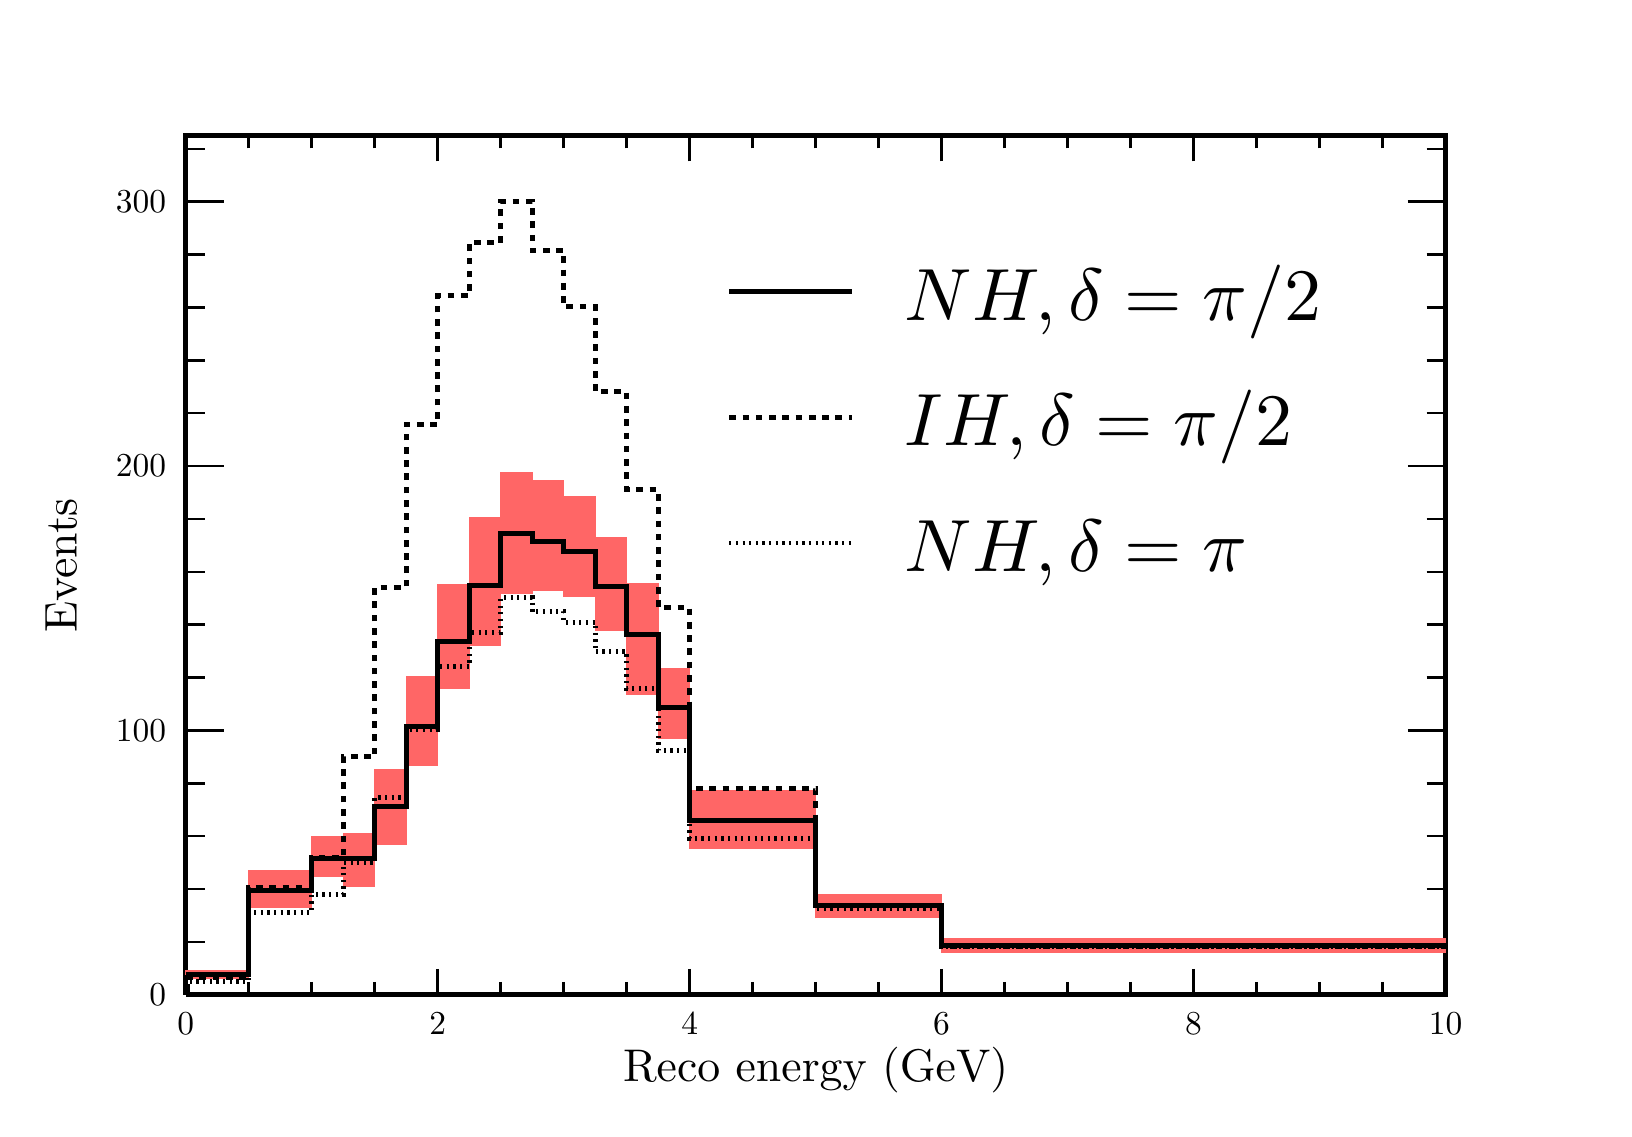
\begin{tikzpicture}
\pgfdeclareplotmark{cross} {
\pgfpathmoveto{\pgfpoint{-0.3\pgfplotmarksize}{\pgfplotmarksize}}
\pgfpathlineto{\pgfpoint{+0.3\pgfplotmarksize}{\pgfplotmarksize}}
\pgfpathlineto{\pgfpoint{+0.3\pgfplotmarksize}{0.3\pgfplotmarksize}}
\pgfpathlineto{\pgfpoint{+1\pgfplotmarksize}{0.3\pgfplotmarksize}}
\pgfpathlineto{\pgfpoint{+1\pgfplotmarksize}{-0.3\pgfplotmarksize}}
\pgfpathlineto{\pgfpoint{+0.3\pgfplotmarksize}{-0.3\pgfplotmarksize}}
\pgfpathlineto{\pgfpoint{+0.3\pgfplotmarksize}{-1.\pgfplotmarksize}}
\pgfpathlineto{\pgfpoint{-0.3\pgfplotmarksize}{-1.\pgfplotmarksize}}
\pgfpathlineto{\pgfpoint{-0.3\pgfplotmarksize}{-0.3\pgfplotmarksize}}
\pgfpathlineto{\pgfpoint{-1.\pgfplotmarksize}{-0.3\pgfplotmarksize}}
\pgfpathlineto{\pgfpoint{-1.\pgfplotmarksize}{0.3\pgfplotmarksize}}
\pgfpathlineto{\pgfpoint{-0.3\pgfplotmarksize}{0.3\pgfplotmarksize}}
\pgfpathclose
\pgfusepathqstroke
}
\pgfdeclareplotmark{cross*} {
\pgfpathmoveto{\pgfpoint{-0.3\pgfplotmarksize}{\pgfplotmarksize}}
\pgfpathlineto{\pgfpoint{+0.3\pgfplotmarksize}{\pgfplotmarksize}}
\pgfpathlineto{\pgfpoint{+0.3\pgfplotmarksize}{0.3\pgfplotmarksize}}
\pgfpathlineto{\pgfpoint{+1\pgfplotmarksize}{0.3\pgfplotmarksize}}
\pgfpathlineto{\pgfpoint{+1\pgfplotmarksize}{-0.3\pgfplotmarksize}}
\pgfpathlineto{\pgfpoint{+0.3\pgfplotmarksize}{-0.3\pgfplotmarksize}}
\pgfpathlineto{\pgfpoint{+0.3\pgfplotmarksize}{-1.\pgfplotmarksize}}
\pgfpathlineto{\pgfpoint{-0.3\pgfplotmarksize}{-1.\pgfplotmarksize}}
\pgfpathlineto{\pgfpoint{-0.3\pgfplotmarksize}{-0.3\pgfplotmarksize}}
\pgfpathlineto{\pgfpoint{-1.\pgfplotmarksize}{-0.3\pgfplotmarksize}}
\pgfpathlineto{\pgfpoint{-1.\pgfplotmarksize}{0.3\pgfplotmarksize}}
\pgfpathlineto{\pgfpoint{-0.3\pgfplotmarksize}{0.3\pgfplotmarksize}}
\pgfpathclose
\pgfusepathqfillstroke
}
\pgfdeclareplotmark{newstar} {
\pgfpathmoveto{\pgfqpoint{0pt}{\pgfplotmarksize}}
\pgfpathlineto{\pgfqpointpolar{44}{0.5\pgfplotmarksize}}
\pgfpathlineto{\pgfqpointpolar{18}{\pgfplotmarksize}}
\pgfpathlineto{\pgfqpointpolar{-20}{0.5\pgfplotmarksize}}
\pgfpathlineto{\pgfqpointpolar{-54}{\pgfplotmarksize}}
\pgfpathlineto{\pgfqpointpolar{-90}{0.5\pgfplotmarksize}}
\pgfpathlineto{\pgfqpointpolar{234}{\pgfplotmarksize}}
\pgfpathlineto{\pgfqpointpolar{198}{0.5\pgfplotmarksize}}
\pgfpathlineto{\pgfqpointpolar{162}{\pgfplotmarksize}}
\pgfpathlineto{\pgfqpointpolar{134}{0.5\pgfplotmarksize}}
\pgfpathclose
\pgfusepathqstroke
}
\pgfdeclareplotmark{newstar*} {
\pgfpathmoveto{\pgfqpoint{0pt}{\pgfplotmarksize}}
\pgfpathlineto{\pgfqpointpolar{44}{0.5\pgfplotmarksize}}
\pgfpathlineto{\pgfqpointpolar{18}{\pgfplotmarksize}}
\pgfpathlineto{\pgfqpointpolar{-20}{0.5\pgfplotmarksize}}
\pgfpathlineto{\pgfqpointpolar{-54}{\pgfplotmarksize}}
\pgfpathlineto{\pgfqpointpolar{-90}{0.5\pgfplotmarksize}}
\pgfpathlineto{\pgfqpointpolar{234}{\pgfplotmarksize}}
\pgfpathlineto{\pgfqpointpolar{198}{0.5\pgfplotmarksize}}
\pgfpathlineto{\pgfqpointpolar{162}{\pgfplotmarksize}}
\pgfpathlineto{\pgfqpointpolar{134}{0.5\pgfplotmarksize}}
\pgfpathclose
\pgfusepathqfillstroke
}
\definecolor{c}{rgb}{0.999,0.999,0.999};
\draw [color=c, fill=c] (0,0) rectangle (20,13.639);
\draw [color=c, fill=c] (2,1.3639) rectangle (18,12.2751);
\definecolor{c}{rgb}{0,0,0};
\draw [c,line width=1.8] (2,1.3639) -- (2,12.2751) -- (18,12.2751) -- (18,1.3639) -- (2,1.3639);
\definecolor{c}{rgb}{0.999,0.999,0.999};
\draw [color=c, fill=c] (2,1.3639) rectangle (18,12.2751);
\definecolor{c}{rgb}{0,0,0};
\draw [c,line width=1.8] (2,1.3639) -- (2,12.2751) -- (18,12.2751) -- (18,1.3639) -- (2,1.3639);
\draw [c,line width=1.8] (2,1.6177) -- (2.8,1.6177) -- (2.8,2.68844) -- (3.6,2.68844) -- (3.6,3.09122) -- (4,3.09122) -- (4,3.08849) -- (4.4,3.08849) -- (4.4,3.75008) -- (4.8,3.75008) -- (4.8,4.76675) -- (5.2,4.76675) -- (5.2,5.85521) --
 (5.6,5.85521) -- (5.6,6.56073) -- (6,6.56073) -- (6,7.21918) -- (6.4,7.21918) -- (6.4,7.12647) -- (6.8,7.12647) -- (6.8,6.99581) -- (7.2,6.99581) -- (7.2,6.54549) -- (7.6,6.54549) -- (7.6,5.94198) -- (8,5.94198) -- (8,5.00812) -- (8.4,5.00812) --
 (8.4,3.57712) -- (10,3.57712) -- (10,2.49612) -- (11.6,2.49612) -- (11.6,1.98899) -- (18,1.98899);
\draw [c,line width=0.9] (2,1.3639) -- (18,1.3639);
\draw [c,line width=0.9] (2,1.69123) -- (2,1.3639);
\draw [c,line width=0.9] (2.8,1.52756) -- (2.8,1.3639);
\draw [c,line width=0.9] (3.6,1.52756) -- (3.6,1.3639);
\draw [c,line width=0.9] (4.4,1.52756) -- (4.4,1.3639);
\draw [c,line width=0.9] (5.2,1.69123) -- (5.2,1.3639);
\draw [c,line width=0.9] (6,1.52756) -- (6,1.3639);
\draw [c,line width=0.9] (6.8,1.52756) -- (6.8,1.3639);
\draw [c,line width=0.9] (7.6,1.52756) -- (7.6,1.3639);
\draw [c,line width=0.9] (8.4,1.69123) -- (8.4,1.3639);
\draw [c,line width=0.9] (9.2,1.52756) -- (9.2,1.3639);
\draw [c,line width=0.9] (10,1.52756) -- (10,1.3639);
\draw [c,line width=0.9] (10.8,1.52756) -- (10.8,1.3639);
\draw [c,line width=0.9] (11.6,1.69123) -- (11.6,1.3639);
\draw [c,line width=0.9] (12.4,1.52756) -- (12.4,1.3639);
\draw [c,line width=0.9] (13.2,1.52756) -- (13.2,1.3639);
\draw [c,line width=0.9] (14,1.52756) -- (14,1.3639);
\draw [c,line width=0.9] (14.8,1.69123) -- (14.8,1.3639);
\draw [c,line width=0.9] (15.6,1.52756) -- (15.6,1.3639);
\draw [c,line width=0.9] (16.4,1.52756) -- (16.4,1.3639);
\draw [c,line width=0.9] (17.2,1.52756) -- (17.2,1.3639);
\draw [c,line width=0.9] (18,1.69123) -- (18,1.3639);
\draw [anchor=base] (2,0.859255) node[scale=1.20912, color=c, rotate=0]{0};
\draw [anchor=base] (5.2,0.859255) node[scale=1.20912, color=c, rotate=0]{2};
\draw [anchor=base] (8.4,0.859255) node[scale=1.20912, color=c, rotate=0]{4};
\draw [anchor=base] (11.6,0.859255) node[scale=1.20912, color=c, rotate=0]{6};
\draw [anchor=base] (14.8,0.859255) node[scale=1.20912, color=c, rotate=0]{8};
\draw [anchor=base] (18,0.859255) node[scale=1.20912, color=c, rotate=0]{10};
\draw (10,0.403714) node[scale=1.65459, color=c, rotate=0]{Reco energy (GeV)};
\draw [c,line width=0.9] (2,12.2751) -- (18,12.2751);
\draw [c,line width=0.9] (2,11.9477) -- (2,12.2751);
\draw [c,line width=0.9] (2.8,12.1114) -- (2.8,12.2751);
\draw [c,line width=0.9] (3.6,12.1114) -- (3.6,12.2751);
\draw [c,line width=0.9] (4.4,12.1114) -- (4.4,12.2751);
\draw [c,line width=0.9] (5.2,11.9477) -- (5.2,12.2751);
\draw [c,line width=0.9] (6,12.1114) -- (6,12.2751);
\draw [c,line width=0.9] (6.8,12.1114) -- (6.8,12.2751);
\draw [c,line width=0.9] (7.6,12.1114) -- (7.6,12.2751);
\draw [c,line width=0.9] (8.4,11.9477) -- (8.4,12.2751);
\draw [c,line width=0.9] (9.2,12.1114) -- (9.2,12.2751);
\draw [c,line width=0.9] (10,12.1114) -- (10,12.2751);
\draw [c,line width=0.9] (10.8,12.1114) -- (10.8,12.2751);
\draw [c,line width=0.9] (11.6,11.9477) -- (11.6,12.2751);
\draw [c,line width=0.9] (12.4,12.1114) -- (12.4,12.2751);
\draw [c,line width=0.9] (13.2,12.1114) -- (13.2,12.2751);
\draw [c,line width=0.9] (14,12.1114) -- (14,12.2751);
\draw [c,line width=0.9] (14.8,11.9477) -- (14.8,12.2751);
\draw [c,line width=0.9] (15.6,12.1114) -- (15.6,12.2751);
\draw [c,line width=0.9] (16.4,12.1114) -- (16.4,12.2751);
\draw [c,line width=0.9] (17.2,12.1114) -- (17.2,12.2751);
\draw [c,line width=0.9] (18,11.9477) -- (18,12.2751);
\draw [c,line width=0.9] (2,1.3639) -- (2,12.2751);
\draw [c,line width=0.9] (2.48,1.3639) -- (2,1.3639);
\draw [c,line width=0.9] (2.24,2.03535) -- (2,2.03535);
\draw [c,line width=0.9] (2.24,2.70681) -- (2,2.70681);
\draw [c,line width=0.9] (2.24,3.37827) -- (2,3.37827);
\draw [c,line width=0.9] (2.24,4.04972) -- (2,4.04972);
\draw [c,line width=0.9] (2.48,4.72118) -- (2,4.72118);
\draw [c,line width=0.9] (2.24,5.39264) -- (2,5.39264);
\draw [c,line width=0.9] (2.24,6.0641) -- (2,6.0641);
\draw [c,line width=0.9] (2.24,6.73555) -- (2,6.73555);
\draw [c,line width=0.9] (2.24,7.40701) -- (2,7.40701);
\draw [c,line width=0.9] (2.48,8.07847) -- (2,8.07847);
\draw [c,line width=0.9] (2.24,8.74992) -- (2,8.74992);
\draw [c,line width=0.9] (2.24,9.42138) -- (2,9.42138);
\draw [c,line width=0.9] (2.24,10.0928) -- (2,10.0928);
\draw [c,line width=0.9] (2.24,10.7643) -- (2,10.7643);
\draw [c,line width=0.9] (2.48,11.4358) -- (2,11.4358);
\draw [c,line width=0.9] (2.48,11.4358) -- (2,11.4358);
\draw [c,line width=0.9] (2.24,12.1072) -- (2,12.1072);
\draw [anchor= east] (1.9,1.3639) node[scale=1.20912, color=c, rotate=0]{0};
\draw [anchor= east] (1.9,4.72118) node[scale=1.20912, color=c, rotate=0]{100};
\draw [anchor= east] (1.9,8.07847) node[scale=1.20912, color=c, rotate=0]{200};
\draw [anchor= east] (1.9,11.4358) node[scale=1.20912, color=c, rotate=0]{300};
\draw (0.416,6.81948) node[scale=1.65459, color=c, rotate=90]{Events};
\draw [c,line width=0.9] (18,1.3639) -- (18,12.2751);
\draw [c,line width=0.9] (17.52,1.3639) -- (18,1.3639);
\draw [c,line width=0.9] (17.76,2.03535) -- (18,2.03535);
\draw [c,line width=0.9] (17.76,2.70681) -- (18,2.70681);
\draw [c,line width=0.9] (17.76,3.37827) -- (18,3.37827);
\draw [c,line width=0.9] (17.76,4.04972) -- (18,4.04972);
\draw [c,line width=0.9] (17.52,4.72118) -- (18,4.72118);
\draw [c,line width=0.9] (17.76,5.39264) -- (18,5.39264);
\draw [c,line width=0.9] (17.76,6.0641) -- (18,6.0641);
\draw [c,line width=0.9] (17.76,6.73555) -- (18,6.73555);
\draw [c,line width=0.9] (17.76,7.40701) -- (18,7.40701);
\draw [c,line width=0.9] (17.52,8.07847) -- (18,8.07847);
\draw [c,line width=0.9] (17.76,8.74992) -- (18,8.74992);
\draw [c,line width=0.9] (17.76,9.42138) -- (18,9.42138);
\draw [c,line width=0.9] (17.76,10.0928) -- (18,10.0928);
\draw [c,line width=0.9] (17.76,10.7643) -- (18,10.7643);
\draw [c,line width=0.9] (17.52,11.4358) -- (18,11.4358);
\draw [c,line width=0.9] (17.52,11.4358) -- (18,11.4358);
\draw [c,line width=0.9] (17.76,12.1072) -- (18,12.1072);
\definecolor{c}{rgb}{1,0.4,0.4};
\draw [color=c, fill=c] (2,1.56583) rectangle (2.8,1.67706);
\draw [color=c, fill=c] (2.8,2.47101) rectangle (3.6,2.93721);
\draw [color=c, fill=c] (3.6,2.86112) rectangle (4,3.3723);
\draw [color=c, fill=c] (4,2.74153) rectangle (4.4,3.40935);
\draw [color=c, fill=c] (4.4,3.27555) rectangle (4.8,4.21832);
\draw [color=c, fill=c] (4.8,4.27587) rectangle (5.2,5.40328);
\draw [color=c, fill=c] (5.2,5.25327) rectangle (5.6,6.57743);
\draw [color=c, fill=c] (5.6,5.80297) rectangle (6,7.42178);
\draw [color=c, fill=c] (6,6.46267) rectangle (6.4,7.99531);
\draw [color=c, fill=c] (6.4,6.4933) rectangle (6.8,7.90008);
\draw [color=c, fill=c] (6.8,6.42671) rectangle (7.2,7.69297);
\draw [color=c, fill=c] (7.2,5.98745) rectangle (7.6,7.16849);
\draw [color=c, fill=c] (7.6,5.17805) rectangle (8,6.58456);
\draw [color=c, fill=c] (8,4.61291) rectangle (8.4,5.51272);
\draw [color=c, fill=c] (8.4,3.2252) rectangle (10,3.9541);
\draw [color=c, fill=c] (10,2.3515) rectangle (11.6,2.64007);
\draw [color=c, fill=c] (11.6,1.89867) rectangle (18,2.08046);
\definecolor{c}{rgb}{0,0,0};
\draw [c,line width=1.8] (2,1.6177) -- (2.8,1.6177) -- (2.8,2.68844) -- (3.6,2.68844) -- (3.6,3.09122) -- (4,3.09122) -- (4,3.08849) -- (4.4,3.08849) -- (4.4,3.75008) -- (4.8,3.75008) -- (4.8,4.76675) -- (5.2,4.76675) -- (5.2,5.85521) --
 (5.6,5.85521) -- (5.6,6.56073) -- (6,6.56073) -- (6,7.21918) -- (6.4,7.21918) -- (6.4,7.12647) -- (6.8,7.12647) -- (6.8,6.99581) -- (7.2,6.99581) -- (7.2,6.54549) -- (7.6,6.54549) -- (7.6,5.94198) -- (8,5.94198) -- (8,5.00812) -- (8.4,5.00812) --
 (8.4,3.57712) -- (10,3.57712) -- (10,2.49612) -- (11.6,2.49612) -- (11.6,1.98899) -- (18,1.98899);
\draw [c,dash pattern=on 2.40pt off 2.40pt ,line width=1.8] (2.02865,1.39255) -- (2.02865,1.58348) -- (2.8,1.58348) -- (2.8,2.72171) -- (3.6,2.72171) -- (3.6,3.10463) -- (4,3.10463) -- (4,4.38373) -- (4.4,4.38373) -- (4.4,6.53775) -- (4.8,6.53775) --
 (4.8,8.6076) -- (5.2,8.6076) -- (5.2,10.2407) -- (5.6,10.2407) -- (5.6,10.9166) -- (6,10.9166) -- (6,11.4413) -- (6.4,11.4413) -- (6.4,10.8176) -- (6.8,10.8176) -- (6.8,10.1021) -- (7.2,10.1021) -- (7.2,9.02097) -- (7.6,9.02097) -- (7.6,7.78272) --
 (8,7.78272) -- (8,6.28234) -- (8.4,6.28234) -- (8.4,3.98728) -- (10,3.98728) -- (10,2.50318) -- (11.6,2.50318) -- (11.6,1.98241) -- (18,1.98241);
\draw [c,dash pattern=on 0.80pt off 1.60pt ,line width=1.8] (2.02865,1.39255) -- (2.02865,1.53772) -- (2.8,1.53772) -- (2.8,2.40784) -- (3.6,2.40784) -- (3.6,2.63669) -- (4,2.63669) -- (4,3.03935) -- (4.4,3.03935) -- (4.4,3.86671) -- (4.8,3.86671) --
 (4.8,4.73566) -- (5.2,4.73566) -- (5.2,5.52994) -- (5.6,5.52994) -- (5.6,5.9674) -- (6,5.9674) -- (6,6.40553) -- (6.4,6.40553) -- (6.4,6.22543) -- (6.8,6.22543) -- (6.8,6.09706) -- (7.2,6.09706) -- (7.2,5.71752) -- (7.6,5.71752) -- (7.6,5.24812) --
 (8,5.24812) -- (8,4.4707) -- (8.4,4.4707) -- (8.4,3.34666) -- (10,3.34666) -- (10,2.45385) -- (11.6,2.45385) -- (11.6,1.97765) -- (18,1.97765);
\definecolor{c}{rgb}{1,1,1};
\draw [color=c, fill=c] (8.56734,6.30372) rectangle (17.5072,11.0888);
\definecolor{c}{rgb}{0,0,0};
\draw [anchor=base west] (10.8023,9.93243) node[scale=2.6728, color=c, rotate=0]{$NH, \delta = \pi/2$};
\draw [c,line width=1.8] (8.90258,10.2913) -- (10.467,10.2913);
\draw [anchor=base west] (10.8023,8.33739) node[scale=2.6728, color=c, rotate=0]{$IH, \delta = \pi/2$};
\draw [c,dash pattern=on 2.40pt off 2.40pt ,line width=1.8] (8.90258,8.69627) -- (10.467,8.69627);
\draw [anchor=base west] (10.8023,6.74236) node[scale=2.6728, color=c, rotate=0]{$NH, \delta = \pi$};
\draw [c,dash pattern=on 0.80pt off 1.60pt ,line width=1.8] (8.90258,7.10124) -- (10.467,7.10124);
\end{tikzpicture}

		\end{adjustbox}
	\end{minipage}
	\caption[DUNE far detector event rates with systematic error bands.]{Event rates for each of the far detector samples. The red band indicates the $\pm1\sigma$ error systematic band for the normal hierarchy, $\dcp = \frac{\pi}{2}$ case. For the \nue event rates, results for different neutrino mass hierarchies and values of \dcp are shown. For the \numu event rates the effect of varying \thetai{23} is between the central value (\ang{49.6}) and a $3\sigma$ error (from Ref.~\cite{nufit4}) is shown. The \numu event rate does not depend on the hierarchy or the value of \dcp. The full MC statistics are used for these plots (with a scaling factor) with no fluctuations so the statistical uncertainty is not shown. Top left: \numu disappearance with the beam in FHC mode. Top right: \numu disappearance with the beam in RHC mode. Bottom left: \nue appearance with the beam in FHC mode. Bottom right: \nue appearance with the beam in RHC mode.}
	\label{fig:fdEventRatesWithErrorBand}
\end{figure}

The two ND samples are two dimensional, binned in reconstructed neutrino energy and reconstructed inelasticity, $y_{\text{reco}}$.
The reconstructed neutrino energy, $E_{\nu,~\text{reco}}$, is calculated by summing the reconstructed energy of the outgoing lepton ($E_{\mu,~\text{reco}}$) and the reconstructed energies of any final state hadrons ($E_{\text{had, reco}}$).
$y_{\text{reco}}$ is defined as
\begin{equation}
	y_{\text{reco}} = \frac{E_{\text{had, reco}}}{ E_{\text{had, reco}} + E_{\mu,~\text{reco}} } \, .
\end{equation}
These two-dimensional samples are shown in \citefig{fig:ndEventRates}.

\begin{figure}[h]
	\begin{minipage}[t]{.5\linewidth}
		\begin{adjustbox}{max totalsize=\linewidth, center}
			\input{files/figures/dune_lbl/h2NDNumuFHC}
		\end{adjustbox}
	\end{minipage}
	\hfill
	\begin{minipage}[t]{.5\linewidth}
		\begin{adjustbox}{max totalsize=\linewidth, center}
			\begin{tikzpicture}
\pgfdeclareplotmark{cross} {
\pgfpathmoveto{\pgfpoint{-0.3\pgfplotmarksize}{\pgfplotmarksize}}
\pgfpathlineto{\pgfpoint{+0.3\pgfplotmarksize}{\pgfplotmarksize}}
\pgfpathlineto{\pgfpoint{+0.3\pgfplotmarksize}{0.3\pgfplotmarksize}}
\pgfpathlineto{\pgfpoint{+1\pgfplotmarksize}{0.3\pgfplotmarksize}}
\pgfpathlineto{\pgfpoint{+1\pgfplotmarksize}{-0.3\pgfplotmarksize}}
\pgfpathlineto{\pgfpoint{+0.3\pgfplotmarksize}{-0.3\pgfplotmarksize}}
\pgfpathlineto{\pgfpoint{+0.3\pgfplotmarksize}{-1.\pgfplotmarksize}}
\pgfpathlineto{\pgfpoint{-0.3\pgfplotmarksize}{-1.\pgfplotmarksize}}
\pgfpathlineto{\pgfpoint{-0.3\pgfplotmarksize}{-0.3\pgfplotmarksize}}
\pgfpathlineto{\pgfpoint{-1.\pgfplotmarksize}{-0.3\pgfplotmarksize}}
\pgfpathlineto{\pgfpoint{-1.\pgfplotmarksize}{0.3\pgfplotmarksize}}
\pgfpathlineto{\pgfpoint{-0.3\pgfplotmarksize}{0.3\pgfplotmarksize}}
\pgfpathclose
\pgfusepathqstroke
}
\pgfdeclareplotmark{cross*} {
\pgfpathmoveto{\pgfpoint{-0.3\pgfplotmarksize}{\pgfplotmarksize}}
\pgfpathlineto{\pgfpoint{+0.3\pgfplotmarksize}{\pgfplotmarksize}}
\pgfpathlineto{\pgfpoint{+0.3\pgfplotmarksize}{0.3\pgfplotmarksize}}
\pgfpathlineto{\pgfpoint{+1\pgfplotmarksize}{0.3\pgfplotmarksize}}
\pgfpathlineto{\pgfpoint{+1\pgfplotmarksize}{-0.3\pgfplotmarksize}}
\pgfpathlineto{\pgfpoint{+0.3\pgfplotmarksize}{-0.3\pgfplotmarksize}}
\pgfpathlineto{\pgfpoint{+0.3\pgfplotmarksize}{-1.\pgfplotmarksize}}
\pgfpathlineto{\pgfpoint{-0.3\pgfplotmarksize}{-1.\pgfplotmarksize}}
\pgfpathlineto{\pgfpoint{-0.3\pgfplotmarksize}{-0.3\pgfplotmarksize}}
\pgfpathlineto{\pgfpoint{-1.\pgfplotmarksize}{-0.3\pgfplotmarksize}}
\pgfpathlineto{\pgfpoint{-1.\pgfplotmarksize}{0.3\pgfplotmarksize}}
\pgfpathlineto{\pgfpoint{-0.3\pgfplotmarksize}{0.3\pgfplotmarksize}}
\pgfpathclose
\pgfusepathqfillstroke
}
\pgfdeclareplotmark{newstar} {
\pgfpathmoveto{\pgfqpoint{0pt}{\pgfplotmarksize}}
\pgfpathlineto{\pgfqpointpolar{44}{0.5\pgfplotmarksize}}
\pgfpathlineto{\pgfqpointpolar{18}{\pgfplotmarksize}}
\pgfpathlineto{\pgfqpointpolar{-20}{0.5\pgfplotmarksize}}
\pgfpathlineto{\pgfqpointpolar{-54}{\pgfplotmarksize}}
\pgfpathlineto{\pgfqpointpolar{-90}{0.5\pgfplotmarksize}}
\pgfpathlineto{\pgfqpointpolar{234}{\pgfplotmarksize}}
\pgfpathlineto{\pgfqpointpolar{198}{0.5\pgfplotmarksize}}
\pgfpathlineto{\pgfqpointpolar{162}{\pgfplotmarksize}}
\pgfpathlineto{\pgfqpointpolar{134}{0.5\pgfplotmarksize}}
\pgfpathclose
\pgfusepathqstroke
}
\pgfdeclareplotmark{newstar*} {
\pgfpathmoveto{\pgfqpoint{0pt}{\pgfplotmarksize}}
\pgfpathlineto{\pgfqpointpolar{44}{0.5\pgfplotmarksize}}
\pgfpathlineto{\pgfqpointpolar{18}{\pgfplotmarksize}}
\pgfpathlineto{\pgfqpointpolar{-20}{0.5\pgfplotmarksize}}
\pgfpathlineto{\pgfqpointpolar{-54}{\pgfplotmarksize}}
\pgfpathlineto{\pgfqpointpolar{-90}{0.5\pgfplotmarksize}}
\pgfpathlineto{\pgfqpointpolar{234}{\pgfplotmarksize}}
\pgfpathlineto{\pgfqpointpolar{198}{0.5\pgfplotmarksize}}
\pgfpathlineto{\pgfqpointpolar{162}{\pgfplotmarksize}}
\pgfpathlineto{\pgfqpointpolar{134}{0.5\pgfplotmarksize}}
\pgfpathclose
\pgfusepathqfillstroke
}
\definecolor{c}{rgb}{1,1,1};
\draw [color=c, fill=c] (0,0) rectangle (20,13.639);
\draw [color=c, fill=c] (3,1.77307) rectangle (16,12.2751);
\definecolor{c}{rgb}{0,0,0};
\draw [c,line width=0.9] (3,1.77307) -- (3,12.2751) -- (16,12.2751) -- (16,1.77307) -- (3,1.77307);
\definecolor{c}{rgb}{1,1,1};
\draw [color=c, fill=c] (3,1.77307) rectangle (16,12.2751);
\definecolor{c}{rgb}{0,0,0};
\draw [c,line width=0.9] (3,1.77307) -- (3,12.2751) -- (16,12.2751) -- (16,1.77307) -- (3,1.77307);
\definecolor{c}{rgb}{0.945984,0.951044,0.850727};
\draw [color=c, fill=c] (3,1.77307) rectangle (3.65,2.82327);
\definecolor{c}{rgb}{0.929791,0.940923,0.577483};
\draw [color=c, fill=c] (3.65,1.77307) rectangle (4.3,2.82327);
\definecolor{c}{rgb}{0.922426,0.933333,0.238725};
\draw [color=c, fill=c] (4.3,1.77307) rectangle (4.625,2.82327);
\definecolor{c}{rgb}{0.907108,0.710294,0.0335784};
\draw [color=c, fill=c] (4.625,1.77307) rectangle (4.95,2.82327);
\definecolor{c}{rgb}{0.632353,0.197059,0.0139706};
\draw [color=c, fill=c] (4.95,1.77307) rectangle (5.275,2.82327);
\definecolor{c}{rgb}{0.308824,0,0.00392157};
\draw [color=c, fill=c] (5.275,1.77307) rectangle (5.6,2.82327);
\definecolor{c}{rgb}{0.0882353,0,0.00196078};
\draw [color=c, fill=c] (5.6,1.77307) rectangle (5.925,2.82327);
\definecolor{c}{rgb}{0.00551471,0,0.000122549};
\draw [color=c, fill=c] (5.925,1.77307) rectangle (6.25,2.82327);
\draw [color=c, fill=c] (6.25,1.77307) rectangle (6.575,2.82327);
\definecolor{c}{rgb}{0.0882353,0,0.00196078};
\draw [color=c, fill=c] (6.575,1.77307) rectangle (6.9,2.82327);
\definecolor{c}{rgb}{0.308824,0,0.00392157};
\draw [color=c, fill=c] (6.9,1.77307) rectangle (7.225,2.82327);
\definecolor{c}{rgb}{0.548897,0.126838,0.00955882};
\draw [color=c, fill=c] (7.225,1.77307) rectangle (7.55,2.82327);
\definecolor{c}{rgb}{0.790196,0.354902,0.0308824};
\draw [color=c, fill=c] (7.55,1.77307) rectangle (7.875,2.82327);
\definecolor{c}{rgb}{0.888726,0.609559,0.0321078};
\draw [color=c, fill=c] (7.875,1.77307) rectangle (8.2,2.82327);
\definecolor{c}{rgb}{0.927206,0.933333,0.104902};
\draw [color=c, fill=c] (8.2,1.77307) rectangle (9.5,2.82327);
\definecolor{c}{rgb}{0.926755,0.939026,0.526249};
\draw [color=c, fill=c] (9.5,1.77307) rectangle (10.8,2.82327);
\definecolor{c}{rgb}{0.936875,0.945351,0.697027};
\draw [color=c, fill=c] (10.8,1.77307) rectangle (16,2.82327);
\definecolor{c}{rgb}{0.945984,0.951044,0.850727};
\draw [color=c, fill=c] (3,2.82327) rectangle (3.65,3.87347);
\definecolor{c}{rgb}{0.933839,0.943453,0.645794};
\draw [color=c, fill=c] (3.65,2.82327) rectangle (4.3,3.87347);
\definecolor{c}{rgb}{0.923719,0.937128,0.475016};
\draw [color=c, fill=c] (4.3,2.82327) rectangle (4.625,3.87347);
\definecolor{c}{rgb}{0.923529,0.933333,0.207843};
\draw [color=c, fill=c] (4.625,2.82327) rectangle (4.95,3.87347);
\definecolor{c}{rgb}{0.904534,0.684559,0.0324755};
\draw [color=c, fill=c] (4.95,2.82327) rectangle (5.275,3.87347);
\definecolor{c}{rgb}{0.762745,0.327451,0.0279412};
\draw [color=c, fill=c] (5.275,2.82327) rectangle (5.6,3.87347);
\definecolor{c}{rgb}{0.590809,0.159926,0.0110294};
\draw [color=c, fill=c] (5.6,2.82327) rectangle (5.925,3.87347);
\definecolor{c}{rgb}{0.520956,0.104779,0.00857843};
\draw [color=c, fill=c] (5.925,2.82327) rectangle (6.25,3.87347);
\definecolor{c}{rgb}{0.590809,0.159926,0.0110294};
\draw [color=c, fill=c] (6.25,2.82327) rectangle (6.575,3.87347);
\definecolor{c}{rgb}{0.721569,0.286275,0.0235294};
\draw [color=c, fill=c] (6.575,2.82327) rectangle (6.9,3.87347);
\definecolor{c}{rgb}{0.853431,0.478186,0.0340686};
\draw [color=c, fill=c] (6.9,2.82327) rectangle (7.225,3.87347);
\definecolor{c}{rgb}{0.904534,0.684559,0.0324755};
\draw [color=c, fill=c] (7.225,2.82327) rectangle (7.55,3.87347);
\definecolor{c}{rgb}{0.923407,0.873284,0.0405637};
\draw [color=c, fill=c] (7.55,2.82327) rectangle (7.875,3.87347);
\definecolor{c}{rgb}{0.926103,0.933333,0.135784};
\draw [color=c, fill=c] (7.875,2.82327) rectangle (8.2,3.87347);
\definecolor{c}{rgb}{0.920683,0.935231,0.423782};
\draw [color=c, fill=c] (8.2,2.82327) rectangle (9.5,3.87347);
\definecolor{c}{rgb}{0.939911,0.947249,0.748261};
\draw [color=c, fill=c] (9.5,2.82327) rectangle (10.8,3.87347);
\definecolor{c}{rgb}{0.942948,0.949146,0.799494};
\draw [color=c, fill=c] (10.8,2.82327) rectangle (16,3.87347);
\definecolor{c}{rgb}{0.945984,0.951044,0.850727};
\draw [color=c, fill=c] (3,3.87347) rectangle (3.65,4.92367);
\definecolor{c}{rgb}{0.933839,0.943453,0.645794};
\draw [color=c, fill=c] (3.65,3.87347) rectangle (4.3,4.92367);
\definecolor{c}{rgb}{0.923719,0.937128,0.475016};
\draw [color=c, fill=c] (4.3,3.87347) rectangle (4.625,4.92367);
\definecolor{c}{rgb}{0.917647,0.933333,0.372549};
\draw [color=c, fill=c] (4.625,3.87347) rectangle (4.95,4.92367);
\definecolor{c}{rgb}{0.923529,0.933333,0.207843};
\draw [color=c, fill=c] (4.95,3.87347) rectangle (5.275,4.92367);
\definecolor{c}{rgb}{0.923407,0.873284,0.0405637};
\draw [color=c, fill=c] (5.275,3.87347) rectangle (5.6,4.92367);
\definecolor{c}{rgb}{0.909681,0.736029,0.0346814};
\draw [color=c, fill=c] (5.6,3.87347) rectangle (5.925,4.92367);
\definecolor{c}{rgb}{0.907108,0.710294,0.0335784};
\draw [color=c, fill=c] (5.925,3.87347) rectangle (6.25,4.92367);
\definecolor{c}{rgb}{0.913113,0.770343,0.036152};
\draw [color=c, fill=c] (6.25,3.87347) rectangle (6.575,4.92367);
\definecolor{c}{rgb}{0.920833,0.847549,0.0394608};
\draw [color=c, fill=c] (6.575,3.87347) rectangle (6.9,4.92367);
\definecolor{c}{rgb}{0.927206,0.933333,0.104902};
\draw [color=c, fill=c] (6.9,3.87347) rectangle (7.225,4.92367);
\definecolor{c}{rgb}{0.922426,0.933333,0.238725};
\draw [color=c, fill=c] (7.225,3.87347) rectangle (7.55,4.92367);
\definecolor{c}{rgb}{0.917647,0.933333,0.372549};
\draw [color=c, fill=c] (7.55,3.87347) rectangle (7.875,4.92367);
\definecolor{c}{rgb}{0.923719,0.937128,0.475016};
\draw [color=c, fill=c] (7.875,3.87347) rectangle (8.2,4.92367);
\definecolor{c}{rgb}{0.936875,0.945351,0.697027};
\draw [color=c, fill=c] (8.2,3.87347) rectangle (9.5,4.92367);
\definecolor{c}{rgb}{0.942948,0.949146,0.799494};
\draw [color=c, fill=c] (9.5,3.87347) rectangle (10.8,4.92367);
\definecolor{c}{rgb}{0.945984,0.951044,0.850727};
\draw [color=c, fill=c] (10.8,3.87347) rectangle (16,4.92367);
\draw [color=c, fill=c] (3,4.92367) rectangle (3.65,5.97387);
\definecolor{c}{rgb}{0.933839,0.943453,0.645794};
\draw [color=c, fill=c] (3.65,4.92367) rectangle (4.3,5.97387);
\definecolor{c}{rgb}{0.926755,0.939026,0.526249};
\draw [color=c, fill=c] (4.3,4.92367) rectangle (4.625,5.97387);
\draw [color=c, fill=c] (4.625,4.92367) rectangle (4.95,5.97387);
\draw [color=c, fill=c] (4.95,4.92367) rectangle (5.275,5.97387);
\definecolor{c}{rgb}{0.917647,0.933333,0.372549};
\draw [color=c, fill=c] (5.275,4.92367) rectangle (5.6,5.97387);
\definecolor{c}{rgb}{0.921324,0.933333,0.269608};
\draw [color=c, fill=c] (5.6,4.92367) rectangle (5.925,5.97387);
\definecolor{c}{rgb}{0.922426,0.933333,0.238725};
\draw [color=c, fill=c] (5.925,4.92367) rectangle (6.25,5.97387);
\definecolor{c}{rgb}{0.921324,0.933333,0.269608};
\draw [color=c, fill=c] (6.25,4.92367) rectangle (6.575,5.97387);
\definecolor{c}{rgb}{0.919118,0.933333,0.331373};
\draw [color=c, fill=c] (6.575,4.92367) rectangle (6.9,5.97387);
\definecolor{c}{rgb}{0.923719,0.937128,0.475016};
\draw [color=c, fill=c] (6.9,4.92367) rectangle (7.225,5.97387);
\definecolor{c}{rgb}{0.929791,0.940923,0.577483};
\draw [color=c, fill=c] (7.225,4.92367) rectangle (7.55,5.97387);
\definecolor{c}{rgb}{0.936875,0.945351,0.697027};
\draw [color=c, fill=c] (7.55,4.92367) rectangle (7.875,5.97387);
\definecolor{c}{rgb}{0.939911,0.947249,0.748261};
\draw [color=c, fill=c] (7.875,4.92367) rectangle (8.2,5.97387);
\definecolor{c}{rgb}{0.942948,0.949146,0.799494};
\draw [color=c, fill=c] (8.2,4.92367) rectangle (9.5,5.97387);
\definecolor{c}{rgb}{0.945984,0.951044,0.850727};
\draw [color=c, fill=c] (9.5,4.92367) rectangle (10.8,5.97387);
\draw [color=c, fill=c] (10.8,4.92367) rectangle (16,5.97387);
\definecolor{c}{rgb}{0.936875,0.945351,0.697027};
\draw [color=c, fill=c] (3.65,5.97387) rectangle (4.3,8.07427);
\definecolor{c}{rgb}{0.929791,0.940923,0.577483};
\draw [color=c, fill=c] (4.3,5.97387) rectangle (4.625,8.07427);
\draw [color=c, fill=c] (4.625,5.97387) rectangle (4.95,8.07427);
\definecolor{c}{rgb}{0.933839,0.943453,0.645794};
\draw [color=c, fill=c] (4.95,5.97387) rectangle (5.275,8.07427);
\definecolor{c}{rgb}{0.936875,0.945351,0.697027};
\draw [color=c, fill=c] (5.275,5.97387) rectangle (5.6,8.07427);
\draw [color=c, fill=c] (5.6,5.97387) rectangle (5.925,8.07427);
\draw [color=c, fill=c] (5.925,5.97387) rectangle (6.25,8.07427);
\definecolor{c}{rgb}{0.939911,0.947249,0.748261};
\draw [color=c, fill=c] (6.25,5.97387) rectangle (6.575,8.07427);
\draw [color=c, fill=c] (6.575,5.97387) rectangle (6.9,8.07427);
\definecolor{c}{rgb}{0.942948,0.949146,0.799494};
\draw [color=c, fill=c] (6.9,5.97387) rectangle (7.225,8.07427);
\draw [color=c, fill=c] (7.225,5.97387) rectangle (7.55,8.07427);
\draw [color=c, fill=c] (7.55,5.97387) rectangle (7.875,8.07427);
\definecolor{c}{rgb}{0.945984,0.951044,0.850727};
\draw [color=c, fill=c] (7.875,5.97387) rectangle (8.2,8.07427);
\draw [color=c, fill=c] (8.2,5.97387) rectangle (9.5,8.07427);
\draw [color=c, fill=c] (9.5,5.97387) rectangle (10.8,8.07427);
\draw [color=c, fill=c] (10.8,5.97387) rectangle (16,8.07427);
\draw [color=c, fill=c] (3,8.07427) rectangle (3.65,12.2751);
\draw [color=c, fill=c] (3.65,8.07427) rectangle (4.3,12.2751);
\definecolor{c}{rgb}{0.942948,0.949146,0.799494};
\draw [color=c, fill=c] (4.3,8.07427) rectangle (4.625,12.2751);
\draw [color=c, fill=c] (4.625,8.07427) rectangle (4.95,12.2751);
\draw [color=c, fill=c] (4.95,8.07427) rectangle (5.275,12.2751);
\draw [color=c, fill=c] (5.275,8.07427) rectangle (5.6,12.2751);
\definecolor{c}{rgb}{0.945984,0.951044,0.850727};
\draw [color=c, fill=c] (5.6,8.07427) rectangle (5.925,12.2751);
\draw [color=c, fill=c] (5.925,8.07427) rectangle (6.25,12.2751);
\draw [color=c, fill=c] (6.25,8.07427) rectangle (6.575,12.2751);
\draw [color=c, fill=c] (6.575,8.07427) rectangle (6.9,12.2751);
\draw [color=c, fill=c] (6.9,8.07427) rectangle (7.225,12.2751);
\draw [color=c, fill=c] (7.225,8.07427) rectangle (7.55,12.2751);
\draw [color=c, fill=c] (7.55,8.07427) rectangle (7.875,12.2751);
\draw [color=c, fill=c] (7.875,8.07427) rectangle (8.2,12.2751);
\draw [color=c, fill=c] (8.2,8.07427) rectangle (9.5,12.2751);
\draw [color=c, fill=c] (9.5,8.07427) rectangle (10.8,12.2751);
\draw [color=c, fill=c] (10.8,8.07427) rectangle (16,12.2751);
\definecolor{c}{rgb}{0,0,0};
\draw [c,line width=0.9] (3,1.77307) -- (16,1.77307);
\draw [c,line width=0.9] (3,2.03903) -- (3,1.77307);
\draw [c,line width=0.9] (3.65,1.90605) -- (3.65,1.77307);
\draw [c,line width=0.9] (4.3,1.90605) -- (4.3,1.77307);
\draw [c,line width=0.9] (4.95,1.90605) -- (4.95,1.77307);
\draw [c,line width=0.9] (5.6,2.03903) -- (5.6,1.77307);
\draw [c,line width=0.9] (6.25,1.90605) -- (6.25,1.77307);
\draw [c,line width=0.9] (6.9,1.90605) -- (6.9,1.77307);
\draw [c,line width=0.9] (7.55,1.90605) -- (7.55,1.77307);
\draw [c,line width=0.9] (8.2,2.03903) -- (8.2,1.77307);
\draw [c,line width=0.9] (8.85,1.90605) -- (8.85,1.77307);
\draw [c,line width=0.9] (9.5,1.90605) -- (9.5,1.77307);
\draw [c,line width=0.9] (10.15,1.90605) -- (10.15,1.77307);
\draw [c,line width=0.9] (10.8,2.03903) -- (10.8,1.77307);
\draw [c,line width=0.9] (11.45,1.90605) -- (11.45,1.77307);
\draw [c,line width=0.9] (12.1,1.90605) -- (12.1,1.77307);
\draw [c,line width=0.9] (12.75,1.90605) -- (12.75,1.77307);
\draw [c,line width=0.9] (13.4,2.03903) -- (13.4,1.77307);
\draw [c,line width=0.9] (14.05,1.90605) -- (14.05,1.77307);
\draw [c,line width=0.9] (14.7,1.90605) -- (14.7,1.77307);
\draw [c,line width=0.9] (15.35,1.90605) -- (15.35,1.77307);
\draw [c,line width=0.9] (16,2.03903) -- (16,1.77307);
\draw [anchor=base] (3,1.15931) node[scale=1.52731, color=c, rotate=0]{0};
\draw [anchor=base] (5.6,1.15931) node[scale=1.52731, color=c, rotate=0]{2};
\draw [anchor=base] (8.2,1.15931) node[scale=1.52731, color=c, rotate=0]{4};
\draw [anchor=base] (10.8,1.15931) node[scale=1.52731, color=c, rotate=0]{6};
\draw [anchor=base] (13.4,1.15931) node[scale=1.52731, color=c, rotate=0]{8};
\draw [anchor=base] (16,1.15931) node[scale=1.52731, color=c, rotate=0]{10};
\draw [anchor= east] (16,0.572837) node[scale=1.52731, color=c, rotate=0]{$E_{\nu~\text{reco}}$ [\si{\GeV}] };
\draw [c,line width=0.9] (3,12.2751) -- (16,12.2751);
\draw [c,line width=0.9] (3,12.0091) -- (3,12.2751);
\draw [c,line width=0.9] (3.65,12.1421) -- (3.65,12.2751);
\draw [c,line width=0.9] (4.3,12.1421) -- (4.3,12.2751);
\draw [c,line width=0.9] (4.95,12.1421) -- (4.95,12.2751);
\draw [c,line width=0.9] (5.6,12.0091) -- (5.6,12.2751);
\draw [c,line width=0.9] (6.25,12.1421) -- (6.25,12.2751);
\draw [c,line width=0.9] (6.9,12.1421) -- (6.9,12.2751);
\draw [c,line width=0.9] (7.55,12.1421) -- (7.55,12.2751);
\draw [c,line width=0.9] (8.2,12.0091) -- (8.2,12.2751);
\draw [c,line width=0.9] (8.85,12.1421) -- (8.85,12.2751);
\draw [c,line width=0.9] (9.5,12.1421) -- (9.5,12.2751);
\draw [c,line width=0.9] (10.15,12.1421) -- (10.15,12.2751);
\draw [c,line width=0.9] (10.8,12.0091) -- (10.8,12.2751);
\draw [c,line width=0.9] (11.45,12.1421) -- (11.45,12.2751);
\draw [c,line width=0.9] (12.1,12.1421) -- (12.1,12.2751);
\draw [c,line width=0.9] (12.75,12.1421) -- (12.75,12.2751);
\draw [c,line width=0.9] (13.4,12.0091) -- (13.4,12.2751);
\draw [c,line width=0.9] (14.05,12.1421) -- (14.05,12.2751);
\draw [c,line width=0.9] (14.7,12.1421) -- (14.7,12.2751);
\draw [c,line width=0.9] (15.35,12.1421) -- (15.35,12.2751);
\draw [c,line width=0.9] (16,12.0091) -- (16,12.2751);
\draw [c,line width=0.9] (3,1.77307) -- (3,12.2751);
\draw [c,line width=0.9] (3.462,1.77307) -- (3,1.77307);
\draw [c,line width=0.9] (3.231,2.29817) -- (3,2.29817);
\draw [c,line width=0.9] (3.231,2.82327) -- (3,2.82327);
\draw [c,line width=0.9] (3.231,3.34837) -- (3,3.34837);
\draw [c,line width=0.9] (3.462,3.87347) -- (3,3.87347);
\draw [c,line width=0.9] (3.231,4.39857) -- (3,4.39857);
\draw [c,line width=0.9] (3.231,4.92367) -- (3,4.92367);
\draw [c,line width=0.9] (3.231,5.44877) -- (3,5.44877);
\draw [c,line width=0.9] (3.462,5.97387) -- (3,5.97387);
\draw [c,line width=0.9] (3.231,6.49897) -- (3,6.49897);
\draw [c,line width=0.9] (3.231,7.02407) -- (3,7.02407);
\draw [c,line width=0.9] (3.231,7.54917) -- (3,7.54917);
\draw [c,line width=0.9] (3.462,8.07427) -- (3,8.07427);
\draw [c,line width=0.9] (3.231,8.59937) -- (3,8.59937);
\draw [c,line width=0.9] (3.231,9.12447) -- (3,9.12447);
\draw [c,line width=0.9] (3.231,9.64957) -- (3,9.64957);
\draw [c,line width=0.9] (3.462,10.1747) -- (3,10.1747);
\draw [c,line width=0.9] (3.231,10.6998) -- (3,10.6998);
\draw [c,line width=0.9] (3.231,11.2249) -- (3,11.2249);
\draw [c,line width=0.9] (3.231,11.75) -- (3,11.75);
\draw [c,line width=0.9] (3.462,12.2751) -- (3,12.2751);
\draw [c,line width=0.9] (3.462,12.2751) -- (3,12.2751);
\draw [anchor= east] (2.9,1.77307) node[scale=1.52731, color=c, rotate=0]{0};
\draw [anchor= east] (2.9,3.87347) node[scale=1.52731, color=c, rotate=0]{0.2};
\draw [anchor= east] (2.9,5.97387) node[scale=1.52731, color=c, rotate=0]{0.4};
\draw [anchor= east] (2.9,8.07427) node[scale=1.52731, color=c, rotate=0]{0.6};
\draw [anchor= east] (2.9,10.1747) node[scale=1.52731, color=c, rotate=0]{0.8};
\draw [anchor= east] (2.9,12.2751) node[scale=1.52731, color=c, rotate=0]{1};
\draw [anchor= east] (1.24,12.2751) node[scale=1.52731, color=c, rotate=90]{$y_{\text{reco}}$};
\draw [c,line width=0.9] (16,1.77307) -- (16,12.2751);
\draw [c,line width=0.9] (15.538,1.77307) -- (16,1.77307);
\draw [c,line width=0.9] (15.769,2.29817) -- (16,2.29817);
\draw [c,line width=0.9] (15.769,2.82327) -- (16,2.82327);
\draw [c,line width=0.9] (15.769,3.34837) -- (16,3.34837);
\draw [c,line width=0.9] (15.538,3.87347) -- (16,3.87347);
\draw [c,line width=0.9] (15.769,4.39857) -- (16,4.39857);
\draw [c,line width=0.9] (15.769,4.92367) -- (16,4.92367);
\draw [c,line width=0.9] (15.769,5.44877) -- (16,5.44877);
\draw [c,line width=0.9] (15.538,5.97387) -- (16,5.97387);
\draw [c,line width=0.9] (15.769,6.49897) -- (16,6.49897);
\draw [c,line width=0.9] (15.769,7.02407) -- (16,7.02407);
\draw [c,line width=0.9] (15.769,7.54917) -- (16,7.54917);
\draw [c,line width=0.9] (15.538,8.07427) -- (16,8.07427);
\draw [c,line width=0.9] (15.769,8.59937) -- (16,8.59937);
\draw [c,line width=0.9] (15.769,9.12447) -- (16,9.12447);
\draw [c,line width=0.9] (15.769,9.64957) -- (16,9.64957);
\draw [c,line width=0.9] (15.538,10.1747) -- (16,10.1747);
\draw [c,line width=0.9] (15.769,10.6998) -- (16,10.6998);
\draw [c,line width=0.9] (15.769,11.2249) -- (16,11.2249);
\draw [c,line width=0.9] (15.769,11.75) -- (16,11.75);
\draw [c,line width=0.9] (15.538,12.2751) -- (16,12.2751);
\draw [c,line width=0.9] (15.538,12.2751) -- (16,12.2751);
\definecolor{c}{rgb}{0.945984,0.951044,0.850727};
\draw [color=c, fill=c] (16.1032,1.79083) rectangle (17.0201,1.92228);
\definecolor{c}{rgb}{0.942948,0.949146,0.799494};
\draw [color=c, fill=c] (16.1032,1.92228) rectangle (17.0201,2.05373);
\definecolor{c}{rgb}{0.939911,0.947249,0.748261};
\draw [color=c, fill=c] (16.1032,2.05373) rectangle (17.0201,2.18517);
\definecolor{c}{rgb}{0.936875,0.945351,0.697027};
\draw [color=c, fill=c] (16.1032,2.18517) rectangle (17.0201,2.31662);
\definecolor{c}{rgb}{0.933839,0.943453,0.645794};
\draw [color=c, fill=c] (16.1032,2.31662) rectangle (17.0201,2.44807);
\definecolor{c}{rgb}{0.929791,0.940923,0.577483};
\draw [color=c, fill=c] (16.1032,2.44807) rectangle (17.0201,2.57951);
\definecolor{c}{rgb}{0.926755,0.939026,0.526249};
\draw [color=c, fill=c] (16.1032,2.57951) rectangle (17.0201,2.71096);
\definecolor{c}{rgb}{0.923719,0.937128,0.475016};
\draw [color=c, fill=c] (16.1032,2.71096) rectangle (17.0201,2.84241);
\definecolor{c}{rgb}{0.920683,0.935231,0.423782};
\draw [color=c, fill=c] (16.1032,2.84241) rectangle (17.0201,2.97385);
\definecolor{c}{rgb}{0.917647,0.933333,0.372549};
\draw [color=c, fill=c] (16.1032,2.97385) rectangle (17.0201,3.1053);
\definecolor{c}{rgb}{0.919118,0.933333,0.331373};
\draw [color=c, fill=c] (16.1032,3.1053) rectangle (17.0201,3.23675);
\definecolor{c}{rgb}{0.920221,0.933333,0.30049};
\draw [color=c, fill=c] (16.1032,3.23675) rectangle (17.0201,3.36819);
\definecolor{c}{rgb}{0.921324,0.933333,0.269608};
\draw [color=c, fill=c] (16.1032,3.36819) rectangle (17.0201,3.49964);
\definecolor{c}{rgb}{0.922426,0.933333,0.238725};
\draw [color=c, fill=c] (16.1032,3.49964) rectangle (17.0201,3.63109);
\definecolor{c}{rgb}{0.923529,0.933333,0.207843};
\draw [color=c, fill=c] (16.1032,3.63109) rectangle (17.0201,3.76254);
\definecolor{c}{rgb}{0.924632,0.933333,0.176961};
\draw [color=c, fill=c] (16.1032,3.76254) rectangle (17.0201,3.89398);
\definecolor{c}{rgb}{0.926103,0.933333,0.135784};
\draw [color=c, fill=c] (16.1032,3.89398) rectangle (17.0201,4.02543);
\definecolor{c}{rgb}{0.927206,0.933333,0.104902};
\draw [color=c, fill=c] (16.1032,4.02543) rectangle (17.0201,4.15688);
\definecolor{c}{rgb}{0.928309,0.933333,0.0740196};
\draw [color=c, fill=c] (16.1032,4.15688) rectangle (17.0201,4.28832);
\definecolor{c}{rgb}{0.929412,0.933333,0.0431373};
\draw [color=c, fill=c] (16.1032,4.28832) rectangle (17.0201,4.41977);
\definecolor{c}{rgb}{0.926838,0.907598,0.0420343};
\draw [color=c, fill=c] (16.1032,4.41977) rectangle (17.0201,4.55122);
\definecolor{c}{rgb}{0.923407,0.873284,0.0405637};
\draw [color=c, fill=c] (16.1032,4.55122) rectangle (17.0201,4.68266);
\definecolor{c}{rgb}{0.920833,0.847549,0.0394608};
\draw [color=c, fill=c] (16.1032,4.68266) rectangle (17.0201,4.81411);
\definecolor{c}{rgb}{0.91826,0.821814,0.0383578};
\draw [color=c, fill=c] (16.1032,4.81411) rectangle (17.0201,4.94556);
\definecolor{c}{rgb}{0.915686,0.796078,0.0372549};
\draw [color=c, fill=c] (16.1032,4.94556) rectangle (17.0201,5.07701);
\definecolor{c}{rgb}{0.913113,0.770343,0.036152};
\draw [color=c, fill=c] (16.1032,5.07701) rectangle (17.0201,5.20845);
\definecolor{c}{rgb}{0.909681,0.736029,0.0346814};
\draw [color=c, fill=c] (16.1032,5.20845) rectangle (17.0201,5.3399);
\definecolor{c}{rgb}{0.907108,0.710294,0.0335784};
\draw [color=c, fill=c] (16.1032,5.3399) rectangle (17.0201,5.47135);
\definecolor{c}{rgb}{0.904534,0.684559,0.0324755};
\draw [color=c, fill=c] (16.1032,5.47135) rectangle (17.0201,5.60279);
\definecolor{c}{rgb}{0.901961,0.658824,0.0313726};
\draw [color=c, fill=c] (16.1032,5.60279) rectangle (17.0201,5.73424);
\definecolor{c}{rgb}{0.895343,0.634191,0.0317402};
\draw [color=c, fill=c] (16.1032,5.73424) rectangle (17.0201,5.86569);
\definecolor{c}{rgb}{0.888726,0.609559,0.0321078};
\draw [color=c, fill=c] (16.1032,5.86569) rectangle (17.0201,5.99713);
\definecolor{c}{rgb}{0.879902,0.576716,0.032598};
\draw [color=c, fill=c] (16.1032,5.99713) rectangle (17.0201,6.12858);
\definecolor{c}{rgb}{0.873284,0.552083,0.0329657};
\draw [color=c, fill=c] (16.1032,6.12858) rectangle (17.0201,6.26003);
\definecolor{c}{rgb}{0.866667,0.527451,0.0333333};
\draw [color=c, fill=c] (16.1032,6.26003) rectangle (17.0201,6.39148);
\definecolor{c}{rgb}{0.860049,0.502819,0.033701};
\draw [color=c, fill=c] (16.1032,6.39148) rectangle (17.0201,6.52292);
\definecolor{c}{rgb}{0.853431,0.478186,0.0340686};
\draw [color=c, fill=c] (16.1032,6.52292) rectangle (17.0201,6.65437);
\definecolor{c}{rgb}{0.844608,0.445343,0.0345588};
\draw [color=c, fill=c] (16.1032,6.65437) rectangle (17.0201,6.78582);
\definecolor{c}{rgb}{0.83799,0.420711,0.0349265};
\draw [color=c, fill=c] (16.1032,6.78582) rectangle (17.0201,6.91726);
\definecolor{c}{rgb}{0.831373,0.396078,0.0352941};
\draw [color=c, fill=c] (16.1032,6.91726) rectangle (17.0201,7.04871);
\definecolor{c}{rgb}{0.810784,0.37549,0.0330882};
\draw [color=c, fill=c] (16.1032,7.04871) rectangle (17.0201,7.18016);
\definecolor{c}{rgb}{0.790196,0.354902,0.0308824};
\draw [color=c, fill=c] (16.1032,7.18016) rectangle (17.0201,7.3116);
\definecolor{c}{rgb}{0.762745,0.327451,0.0279412};
\draw [color=c, fill=c] (16.1032,7.3116) rectangle (17.0201,7.44305);
\definecolor{c}{rgb}{0.742157,0.306863,0.0257353};
\draw [color=c, fill=c] (16.1032,7.44305) rectangle (17.0201,7.5745);
\definecolor{c}{rgb}{0.721569,0.286275,0.0235294};
\draw [color=c, fill=c] (16.1032,7.5745) rectangle (17.0201,7.70595);
\definecolor{c}{rgb}{0.70098,0.265686,0.0213235};
\draw [color=c, fill=c] (16.1032,7.70595) rectangle (17.0201,7.83739);
\definecolor{c}{rgb}{0.680392,0.245098,0.0191176};
\draw [color=c, fill=c] (16.1032,7.83739) rectangle (17.0201,7.96884);
\definecolor{c}{rgb}{0.659804,0.22451,0.0169118};
\draw [color=c, fill=c] (16.1032,7.96884) rectangle (17.0201,8.10029);
\definecolor{c}{rgb}{0.632353,0.197059,0.0139706};
\draw [color=c, fill=c] (16.1032,8.10029) rectangle (17.0201,8.23173);
\definecolor{c}{rgb}{0.611765,0.176471,0.0117647};
\draw [color=c, fill=c] (16.1032,8.23173) rectangle (17.0201,8.36318);
\definecolor{c}{rgb}{0.590809,0.159926,0.0110294};
\draw [color=c, fill=c] (16.1032,8.36318) rectangle (17.0201,8.49463);
\definecolor{c}{rgb}{0.569853,0.143382,0.0102941};
\draw [color=c, fill=c] (16.1032,8.49463) rectangle (17.0201,8.62607);
\definecolor{c}{rgb}{0.548897,0.126838,0.00955882};
\draw [color=c, fill=c] (16.1032,8.62607) rectangle (17.0201,8.75752);
\definecolor{c}{rgb}{0.520956,0.104779,0.00857843};
\draw [color=c, fill=c] (16.1032,8.75752) rectangle (17.0201,8.88897);
\definecolor{c}{rgb}{0.5,0.0882353,0.00784314};
\draw [color=c, fill=c] (16.1032,8.88897) rectangle (17.0201,9.02042);
\definecolor{c}{rgb}{0.479044,0.0716912,0.00710784};
\draw [color=c, fill=c] (16.1032,9.02042) rectangle (17.0201,9.15186);
\definecolor{c}{rgb}{0.458088,0.0551471,0.00637255};
\draw [color=c, fill=c] (16.1032,9.15186) rectangle (17.0201,9.28331);
\definecolor{c}{rgb}{0.437132,0.0386029,0.00563726};
\draw [color=c, fill=c] (16.1032,9.28331) rectangle (17.0201,9.41476);
\definecolor{c}{rgb}{0.409191,0.0165441,0.00465686};
\draw [color=c, fill=c] (16.1032,9.41476) rectangle (17.0201,9.5462);
\definecolor{c}{rgb}{0.388235,0,0.00392157};
\draw [color=c, fill=c] (16.1032,9.5462) rectangle (17.0201,9.67765);
\definecolor{c}{rgb}{0.368382,0,0.00392157};
\draw [color=c, fill=c] (16.1032,9.67765) rectangle (17.0201,9.8091);
\definecolor{c}{rgb}{0.348529,0,0.00392157};
\draw [color=c, fill=c] (16.1032,9.8091) rectangle (17.0201,9.94054);
\definecolor{c}{rgb}{0.328676,0,0.00392157};
\draw [color=c, fill=c] (16.1032,9.94054) rectangle (17.0201,10.072);
\definecolor{c}{rgb}{0.308824,0,0.00392157};
\draw [color=c, fill=c] (16.1032,10.072) rectangle (17.0201,10.2034);
\definecolor{c}{rgb}{0.282353,0,0.00392157};
\draw [color=c, fill=c] (16.1032,10.2034) rectangle (17.0201,10.3349);
\definecolor{c}{rgb}{0.2625,0,0.00392157};
\draw [color=c, fill=c] (16.1032,10.3349) rectangle (17.0201,10.4663);
\definecolor{c}{rgb}{0.242647,0,0.00392157};
\draw [color=c, fill=c] (16.1032,10.4663) rectangle (17.0201,10.5978);
\definecolor{c}{rgb}{0.222794,0,0.00392157};
\draw [color=c, fill=c] (16.1032,10.5978) rectangle (17.0201,10.7292);
\definecolor{c}{rgb}{0.202941,0,0.00392157};
\draw [color=c, fill=c] (16.1032,10.7292) rectangle (17.0201,10.8607);
\definecolor{c}{rgb}{0.176471,0,0.00392157};
\draw [color=c, fill=c] (16.1032,10.8607) rectangle (17.0201,10.9921);
\definecolor{c}{rgb}{0.159926,0,0.00355392};
\draw [color=c, fill=c] (16.1032,10.9921) rectangle (17.0201,11.1236);
\definecolor{c}{rgb}{0.143382,0,0.00318627};
\draw [color=c, fill=c] (16.1032,11.1236) rectangle (17.0201,11.255);
\definecolor{c}{rgb}{0.126838,0,0.00281863};
\draw [color=c, fill=c] (16.1032,11.255) rectangle (17.0201,11.3865);
\definecolor{c}{rgb}{0.110294,0,0.00245098};
\draw [color=c, fill=c] (16.1032,11.3865) rectangle (17.0201,11.5179);
\definecolor{c}{rgb}{0.0882353,0,0.00196078};
\draw [color=c, fill=c] (16.1032,11.5179) rectangle (17.0201,11.6494);
\definecolor{c}{rgb}{0.0716912,0,0.00159314};
\draw [color=c, fill=c] (16.1032,11.6494) rectangle (17.0201,11.7808);
\definecolor{c}{rgb}{0.0551471,0,0.00122549};
\draw [color=c, fill=c] (16.1032,11.7808) rectangle (17.0201,11.9122);
\definecolor{c}{rgb}{0.0386029,0,0.000857843};
\draw [color=c, fill=c] (16.1032,11.9122) rectangle (17.0201,12.0437);
\definecolor{c}{rgb}{0.0220588,0,0.000490196};
\draw [color=c, fill=c] (16.1032,12.0437) rectangle (17.0201,12.1751);
\definecolor{c}{rgb}{0.00551471,0,0.000122549};
\draw [color=c, fill=c] (16.1032,12.1751) rectangle (17.0201,12.3066);
\definecolor{c}{rgb}{0,0,0};
\draw [c,line width=0.9] (17.0201,1.79083) -- (17.0201,12.3066);
\draw [c,line width=0.9] (16.5575,1.79083) -- (17.0201,1.79083);
\draw [c,line width=0.9] (16.5575,4.22381) -- (17.0201,4.22381);
\draw [c,line width=0.9] (16.5575,6.65679) -- (17.0201,6.65679);
\draw [c,line width=0.9] (16.5575,9.08976) -- (17.0201,9.08976);
\draw [c,line width=0.9] (16.5575,11.5227) -- (17.0201,11.5227);
\draw [c,line width=0.9] (16.5575,11.5227) -- (17.0201,11.5227);
\draw [anchor= west] (17.1201,1.79083) node[scale=1.52731, color=c, rotate=0]{0};
\draw [anchor= west] (17.1201,4.22381) node[scale=1.52731, color=c, rotate=0]{2000};
\draw [anchor= west] (17.1201,6.65679) node[scale=1.52731, color=c, rotate=0]{4000};
\draw [anchor= west] (17.1201,9.08976) node[scale=1.52731, color=c, rotate=0]{6000};
\draw [anchor= west] (17.1201,11.5227) node[scale=1.52731, color=c, rotate=0]{8000};
\draw [anchor=base west] (17.0201,12.3748) node[scale=1.52731, color=c, rotate=0]{$\times10^{3}$};
\draw [anchor= east] (19.1001,12.3066) node[scale=1.52731, color=c, rotate=90]{Events / \si{\GeV} / \si{\year} };
\end{tikzpicture}

		\end{adjustbox}
	\end{minipage}
	\caption[Two-dimensional DUNE ND event rates used in the long-baseline analysis]{Two-dimensional DUNE ND event rates used in the long-baseline analysis. Left: Sample with the beam in neutrino mode. Right: Sample with the beam in antineutrino mode.}
	\label{fig:ndEventRates}
\end{figure}

One-dimensional projections of the samples shown in \citefig{fig:ndEventRates} are shown in \citefig{fig:ndEventRatesWithError} along with the $\pm1\sigma$ error band generated by the systematic uncertainties.
\begin{figure}
	\begin{minipage}[t]{.5\linewidth}
		\begin{adjustbox}{max totalsize=\linewidth, center}
			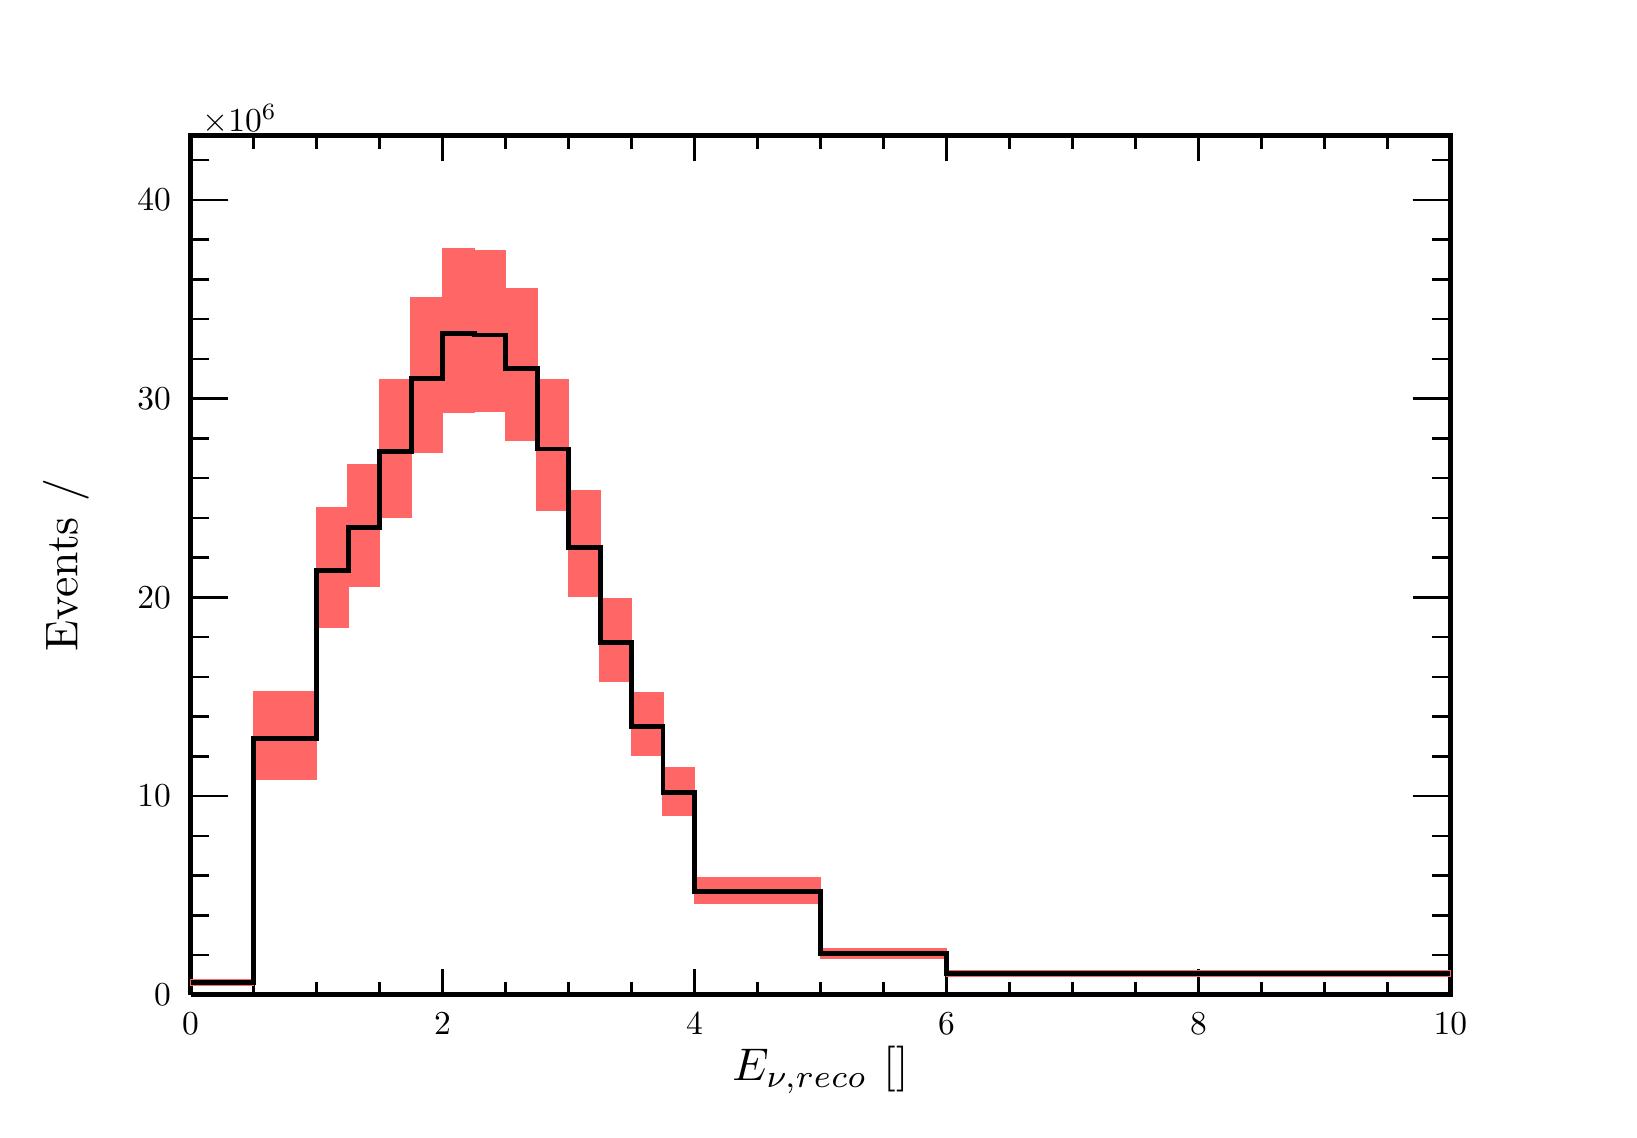
\begin{tikzpicture}
\pgfdeclareplotmark{cross} {
\pgfpathmoveto{\pgfpoint{-0.3\pgfplotmarksize}{\pgfplotmarksize}}
\pgfpathlineto{\pgfpoint{+0.3\pgfplotmarksize}{\pgfplotmarksize}}
\pgfpathlineto{\pgfpoint{+0.3\pgfplotmarksize}{0.3\pgfplotmarksize}}
\pgfpathlineto{\pgfpoint{+1\pgfplotmarksize}{0.3\pgfplotmarksize}}
\pgfpathlineto{\pgfpoint{+1\pgfplotmarksize}{-0.3\pgfplotmarksize}}
\pgfpathlineto{\pgfpoint{+0.3\pgfplotmarksize}{-0.3\pgfplotmarksize}}
\pgfpathlineto{\pgfpoint{+0.3\pgfplotmarksize}{-1.\pgfplotmarksize}}
\pgfpathlineto{\pgfpoint{-0.3\pgfplotmarksize}{-1.\pgfplotmarksize}}
\pgfpathlineto{\pgfpoint{-0.3\pgfplotmarksize}{-0.3\pgfplotmarksize}}
\pgfpathlineto{\pgfpoint{-1.\pgfplotmarksize}{-0.3\pgfplotmarksize}}
\pgfpathlineto{\pgfpoint{-1.\pgfplotmarksize}{0.3\pgfplotmarksize}}
\pgfpathlineto{\pgfpoint{-0.3\pgfplotmarksize}{0.3\pgfplotmarksize}}
\pgfpathclose
\pgfusepathqstroke
}
\pgfdeclareplotmark{cross*} {
\pgfpathmoveto{\pgfpoint{-0.3\pgfplotmarksize}{\pgfplotmarksize}}
\pgfpathlineto{\pgfpoint{+0.3\pgfplotmarksize}{\pgfplotmarksize}}
\pgfpathlineto{\pgfpoint{+0.3\pgfplotmarksize}{0.3\pgfplotmarksize}}
\pgfpathlineto{\pgfpoint{+1\pgfplotmarksize}{0.3\pgfplotmarksize}}
\pgfpathlineto{\pgfpoint{+1\pgfplotmarksize}{-0.3\pgfplotmarksize}}
\pgfpathlineto{\pgfpoint{+0.3\pgfplotmarksize}{-0.3\pgfplotmarksize}}
\pgfpathlineto{\pgfpoint{+0.3\pgfplotmarksize}{-1.\pgfplotmarksize}}
\pgfpathlineto{\pgfpoint{-0.3\pgfplotmarksize}{-1.\pgfplotmarksize}}
\pgfpathlineto{\pgfpoint{-0.3\pgfplotmarksize}{-0.3\pgfplotmarksize}}
\pgfpathlineto{\pgfpoint{-1.\pgfplotmarksize}{-0.3\pgfplotmarksize}}
\pgfpathlineto{\pgfpoint{-1.\pgfplotmarksize}{0.3\pgfplotmarksize}}
\pgfpathlineto{\pgfpoint{-0.3\pgfplotmarksize}{0.3\pgfplotmarksize}}
\pgfpathclose
\pgfusepathqfillstroke
}
\pgfdeclareplotmark{newstar} {
\pgfpathmoveto{\pgfqpoint{0pt}{\pgfplotmarksize}}
\pgfpathlineto{\pgfqpointpolar{44}{0.5\pgfplotmarksize}}
\pgfpathlineto{\pgfqpointpolar{18}{\pgfplotmarksize}}
\pgfpathlineto{\pgfqpointpolar{-20}{0.5\pgfplotmarksize}}
\pgfpathlineto{\pgfqpointpolar{-54}{\pgfplotmarksize}}
\pgfpathlineto{\pgfqpointpolar{-90}{0.5\pgfplotmarksize}}
\pgfpathlineto{\pgfqpointpolar{234}{\pgfplotmarksize}}
\pgfpathlineto{\pgfqpointpolar{198}{0.5\pgfplotmarksize}}
\pgfpathlineto{\pgfqpointpolar{162}{\pgfplotmarksize}}
\pgfpathlineto{\pgfqpointpolar{134}{0.5\pgfplotmarksize}}
\pgfpathclose
\pgfusepathqstroke
}
\pgfdeclareplotmark{newstar*} {
\pgfpathmoveto{\pgfqpoint{0pt}{\pgfplotmarksize}}
\pgfpathlineto{\pgfqpointpolar{44}{0.5\pgfplotmarksize}}
\pgfpathlineto{\pgfqpointpolar{18}{\pgfplotmarksize}}
\pgfpathlineto{\pgfqpointpolar{-20}{0.5\pgfplotmarksize}}
\pgfpathlineto{\pgfqpointpolar{-54}{\pgfplotmarksize}}
\pgfpathlineto{\pgfqpointpolar{-90}{0.5\pgfplotmarksize}}
\pgfpathlineto{\pgfqpointpolar{234}{\pgfplotmarksize}}
\pgfpathlineto{\pgfqpointpolar{198}{0.5\pgfplotmarksize}}
\pgfpathlineto{\pgfqpointpolar{162}{\pgfplotmarksize}}
\pgfpathlineto{\pgfqpointpolar{134}{0.5\pgfplotmarksize}}
\pgfpathclose
\pgfusepathqfillstroke
}
\definecolor{c}{rgb}{0.999,0.999,0.999};
\draw [color=c, fill=c] (0,0) rectangle (20,13.639);
\draw [color=c, fill=c] (2,1.3639) rectangle (18,12.2751);
\definecolor{c}{rgb}{0,0,0};
\draw [c,line width=1.8] (2,1.3639) -- (2,12.2751) -- (18,12.2751) -- (18,1.3639) -- (2,1.3639);
\definecolor{c}{rgb}{0.999,0.999,0.999};
\draw [color=c, fill=c] (2,1.3639) rectangle (18,12.2751);
\definecolor{c}{rgb}{0,0,0};
\draw [c,line width=1.8] (2,1.3639) -- (2,12.2751) -- (18,12.2751) -- (18,1.3639) -- (2,1.3639);
\draw [c,line width=1.8] (2,1.51493) -- (2.8,1.51493) -- (2.8,4.62211) -- (3.6,4.62211) -- (3.6,6.74706) -- (4,6.74706) -- (4,7.2923) -- (4.4,7.2923) -- (4.4,8.26899) -- (4.8,8.26899) -- (4.8,9.19574) -- (5.2,9.19574) -- (5.2,9.75711) --
 (5.6,9.75711) -- (5.6,9.74279) -- (6,9.74279) -- (6,9.31443) -- (6.4,9.31443) -- (6.4,8.29504) -- (6.8,8.29504) -- (6.8,7.04862) -- (7.2,7.04862) -- (7.2,5.83584) -- (7.6,5.83584) -- (7.6,4.77677) -- (8,4.77677) -- (8,3.92868) -- (8.4,3.92868) --
 (8.4,2.68015) -- (10,2.68015) -- (10,1.88528) -- (11.6,1.88528) -- (11.6,1.63144) -- (18,1.63144);
\draw [c,line width=0.9] (2,1.3639) -- (18,1.3639);
\draw [c,line width=0.9] (2,1.69123) -- (2,1.3639);
\draw [c,line width=0.9] (2.8,1.52756) -- (2.8,1.3639);
\draw [c,line width=0.9] (3.6,1.52756) -- (3.6,1.3639);
\draw [c,line width=0.9] (4.4,1.52756) -- (4.4,1.3639);
\draw [c,line width=0.9] (5.2,1.69123) -- (5.2,1.3639);
\draw [c,line width=0.9] (6,1.52756) -- (6,1.3639);
\draw [c,line width=0.9] (6.8,1.52756) -- (6.8,1.3639);
\draw [c,line width=0.9] (7.6,1.52756) -- (7.6,1.3639);
\draw [c,line width=0.9] (8.4,1.69123) -- (8.4,1.3639);
\draw [c,line width=0.9] (9.2,1.52756) -- (9.2,1.3639);
\draw [c,line width=0.9] (10,1.52756) -- (10,1.3639);
\draw [c,line width=0.9] (10.8,1.52756) -- (10.8,1.3639);
\draw [c,line width=0.9] (11.6,1.69123) -- (11.6,1.3639);
\draw [c,line width=0.9] (12.4,1.52756) -- (12.4,1.3639);
\draw [c,line width=0.9] (13.2,1.52756) -- (13.2,1.3639);
\draw [c,line width=0.9] (14,1.52756) -- (14,1.3639);
\draw [c,line width=0.9] (14.8,1.69123) -- (14.8,1.3639);
\draw [c,line width=0.9] (15.6,1.52756) -- (15.6,1.3639);
\draw [c,line width=0.9] (16.4,1.52756) -- (16.4,1.3639);
\draw [c,line width=0.9] (17.2,1.52756) -- (17.2,1.3639);
\draw [c,line width=0.9] (18,1.69123) -- (18,1.3639);
\draw [anchor=base] (2,0.859255) node[scale=1.20912, color=c, rotate=0]{0};
\draw [anchor=base] (5.2,0.859255) node[scale=1.20912, color=c, rotate=0]{2};
\draw [anchor=base] (8.4,0.859255) node[scale=1.20912, color=c, rotate=0]{4};
\draw [anchor=base] (11.6,0.859255) node[scale=1.20912, color=c, rotate=0]{6};
\draw [anchor=base] (14.8,0.859255) node[scale=1.20912, color=c, rotate=0]{8};
\draw [anchor=base] (18,0.859255) node[scale=1.20912, color=c, rotate=0]{10};
\draw (10,0.403714) node[scale=1.65459, color=c, rotate=0]{$E_{\nu, \text{reco}}$ [\si{\GeV}]};
\draw [c,line width=0.9] (2,12.2751) -- (18,12.2751);
\draw [c,line width=0.9] (2,11.9477) -- (2,12.2751);
\draw [c,line width=0.9] (2.8,12.1114) -- (2.8,12.2751);
\draw [c,line width=0.9] (3.6,12.1114) -- (3.6,12.2751);
\draw [c,line width=0.9] (4.4,12.1114) -- (4.4,12.2751);
\draw [c,line width=0.9] (5.2,11.9477) -- (5.2,12.2751);
\draw [c,line width=0.9] (6,12.1114) -- (6,12.2751);
\draw [c,line width=0.9] (6.8,12.1114) -- (6.8,12.2751);
\draw [c,line width=0.9] (7.6,12.1114) -- (7.6,12.2751);
\draw [c,line width=0.9] (8.4,11.9477) -- (8.4,12.2751);
\draw [c,line width=0.9] (9.2,12.1114) -- (9.2,12.2751);
\draw [c,line width=0.9] (10,12.1114) -- (10,12.2751);
\draw [c,line width=0.9] (10.8,12.1114) -- (10.8,12.2751);
\draw [c,line width=0.9] (11.6,11.9477) -- (11.6,12.2751);
\draw [c,line width=0.9] (12.4,12.1114) -- (12.4,12.2751);
\draw [c,line width=0.9] (13.2,12.1114) -- (13.2,12.2751);
\draw [c,line width=0.9] (14,12.1114) -- (14,12.2751);
\draw [c,line width=0.9] (14.8,11.9477) -- (14.8,12.2751);
\draw [c,line width=0.9] (15.6,12.1114) -- (15.6,12.2751);
\draw [c,line width=0.9] (16.4,12.1114) -- (16.4,12.2751);
\draw [c,line width=0.9] (17.2,12.1114) -- (17.2,12.2751);
\draw [c,line width=0.9] (18,11.9477) -- (18,12.2751);
\draw [c,line width=0.9] (2,1.3639) -- (2,12.2751);
\draw [c,line width=0.9] (2.48,1.3639) -- (2,1.3639);
\draw [c,line width=0.9] (2.24,1.86859) -- (2,1.86859);
\draw [c,line width=0.9] (2.24,2.37329) -- (2,2.37329);
\draw [c,line width=0.9] (2.24,2.87799) -- (2,2.87799);
\draw [c,line width=0.9] (2.24,3.38268) -- (2,3.38268);
\draw [c,line width=0.9] (2.48,3.88738) -- (2,3.88738);
\draw [c,line width=0.9] (2.24,4.39208) -- (2,4.39208);
\draw [c,line width=0.9] (2.24,4.89677) -- (2,4.89677);
\draw [c,line width=0.9] (2.24,5.40147) -- (2,5.40147);
\draw [c,line width=0.9] (2.24,5.90617) -- (2,5.90617);
\draw [c,line width=0.9] (2.48,6.41086) -- (2,6.41086);
\draw [c,line width=0.9] (2.24,6.91556) -- (2,6.91556);
\draw [c,line width=0.9] (2.24,7.42026) -- (2,7.42026);
\draw [c,line width=0.9] (2.24,7.92495) -- (2,7.92495);
\draw [c,line width=0.9] (2.24,8.42965) -- (2,8.42965);
\draw [c,line width=0.9] (2.48,8.93435) -- (2,8.93435);
\draw [c,line width=0.9] (2.24,9.43904) -- (2,9.43904);
\draw [c,line width=0.9] (2.24,9.94374) -- (2,9.94374);
\draw [c,line width=0.9] (2.24,10.4484) -- (2,10.4484);
\draw [c,line width=0.9] (2.24,10.9531) -- (2,10.9531);
\draw [c,line width=0.9] (2.48,11.4578) -- (2,11.4578);
\draw [c,line width=0.9] (2.48,11.4578) -- (2,11.4578);
\draw [c,line width=0.9] (2.24,11.9625) -- (2,11.9625);
\draw [anchor= east] (1.9,1.3639) node[scale=1.20912, color=c, rotate=0]{0};
\draw [anchor= east] (1.9,3.88738) node[scale=1.20912, color=c, rotate=0]{10};
\draw [anchor= east] (1.9,6.41086) node[scale=1.20912, color=c, rotate=0]{20};
\draw [anchor= east] (1.9,8.93435) node[scale=1.20912, color=c, rotate=0]{30};
\draw [anchor= east] (1.9,11.4578) node[scale=1.20912, color=c, rotate=0]{40};
\draw [anchor=base west] (2,12.3296) node[scale=1.20912, color=c, rotate=0]{$\times10^{6}$};
\draw (0.416,6.81948) node[scale=1.65459, color=c, rotate=90]{Events / \si{\GeV}};
\draw [c,line width=0.9] (18,1.3639) -- (18,12.2751);
\draw [c,line width=0.9] (17.52,1.3639) -- (18,1.3639);
\draw [c,line width=0.9] (17.76,1.86859) -- (18,1.86859);
\draw [c,line width=0.9] (17.76,2.37329) -- (18,2.37329);
\draw [c,line width=0.9] (17.76,2.87799) -- (18,2.87799);
\draw [c,line width=0.9] (17.76,3.38268) -- (18,3.38268);
\draw [c,line width=0.9] (17.52,3.88738) -- (18,3.88738);
\draw [c,line width=0.9] (17.76,4.39208) -- (18,4.39208);
\draw [c,line width=0.9] (17.76,4.89677) -- (18,4.89677);
\draw [c,line width=0.9] (17.76,5.40147) -- (18,5.40147);
\draw [c,line width=0.9] (17.76,5.90617) -- (18,5.90617);
\draw [c,line width=0.9] (17.52,6.41086) -- (18,6.41086);
\draw [c,line width=0.9] (17.76,6.91556) -- (18,6.91556);
\draw [c,line width=0.9] (17.76,7.42026) -- (18,7.42026);
\draw [c,line width=0.9] (17.76,7.92495) -- (18,7.92495);
\draw [c,line width=0.9] (17.76,8.42965) -- (18,8.42965);
\draw [c,line width=0.9] (17.52,8.93435) -- (18,8.93435);
\draw [c,line width=0.9] (17.76,9.43904) -- (18,9.43904);
\draw [c,line width=0.9] (17.76,9.94374) -- (18,9.94374);
\draw [c,line width=0.9] (17.76,10.4484) -- (18,10.4484);
\draw [c,line width=0.9] (17.76,10.9531) -- (18,10.9531);
\draw [c,line width=0.9] (17.52,11.4578) -- (18,11.4578);
\draw [c,line width=0.9] (17.52,11.4578) -- (18,11.4578);
\draw [c,line width=0.9] (17.76,11.9625) -- (18,11.9625);
\definecolor{c}{rgb}{1,0.4,0.4};
\draw [color=c, fill=c] (2,1.48034) rectangle (2.8,1.55148);
\draw [color=c, fill=c] (2.8,4.10305) rectangle (3.6,5.21699);
\draw [color=c, fill=c] (3.6,6.03199) rectangle (4,7.54785);
\draw [color=c, fill=c] (4,6.54917) rectangle (4.4,8.10234);
\draw [color=c, fill=c] (4.4,7.42277) rectangle (4.8,9.17979);
\draw [color=c, fill=c] (4.8,8.25416) rectangle (5.2,10.2134);
\draw [color=c, fill=c] (5.2,8.76516) rectangle (5.6,10.8389);
\draw [color=c, fill=c] (5.6,8.76627) rectangle (6,10.8176);
\draw [color=c, fill=c] (6,8.39864) rectangle (6.4,10.3341);
\draw [color=c, fill=c] (6.4,7.51232) rectangle (6.8,9.1725);
\draw [color=c, fill=c] (6.8,6.41696) rectangle (7.2,7.76296);
\draw [color=c, fill=c] (7.2,5.34104) rectangle (7.6,6.40042);
\draw [color=c, fill=c] (7.6,4.40155) rectangle (8,5.20583);
\draw [color=c, fill=c] (8,3.64328) rectangle (8.4,4.25281);
\draw [color=c, fill=c] (8.4,2.52743) rectangle (10,2.85207);
\draw [color=c, fill=c] (10,1.82219) rectangle (11.6,1.95458);
\draw [color=c, fill=c] (11.6,1.59807) rectangle (18,1.66732);
\definecolor{c}{rgb}{0,0,0};
\draw [c,line width=1.8] (2,1.51493) -- (2.8,1.51493) -- (2.8,4.62211) -- (3.6,4.62211) -- (3.6,6.74706) -- (4,6.74706) -- (4,7.2923) -- (4.4,7.2923) -- (4.4,8.26899) -- (4.8,8.26899) -- (4.8,9.19574) -- (5.2,9.19574) -- (5.2,9.75711) --
 (5.6,9.75711) -- (5.6,9.74279) -- (6,9.74279) -- (6,9.31443) -- (6.4,9.31443) -- (6.4,8.29504) -- (6.8,8.29504) -- (6.8,7.04862) -- (7.2,7.04862) -- (7.2,5.83584) -- (7.6,5.83584) -- (7.6,4.77677) -- (8,4.77677) -- (8,3.92868) -- (8.4,3.92868) --
 (8.4,2.68015) -- (10,2.68015) -- (10,1.88528) -- (11.6,1.88528) -- (11.6,1.63144) -- (18,1.63144);
\end{tikzpicture}
	
		\end{adjustbox}
	\end{minipage}
	\hfill
	\begin{minipage}[t]{.5\linewidth}
		\begin{adjustbox}{max totalsize=\linewidth, center}
			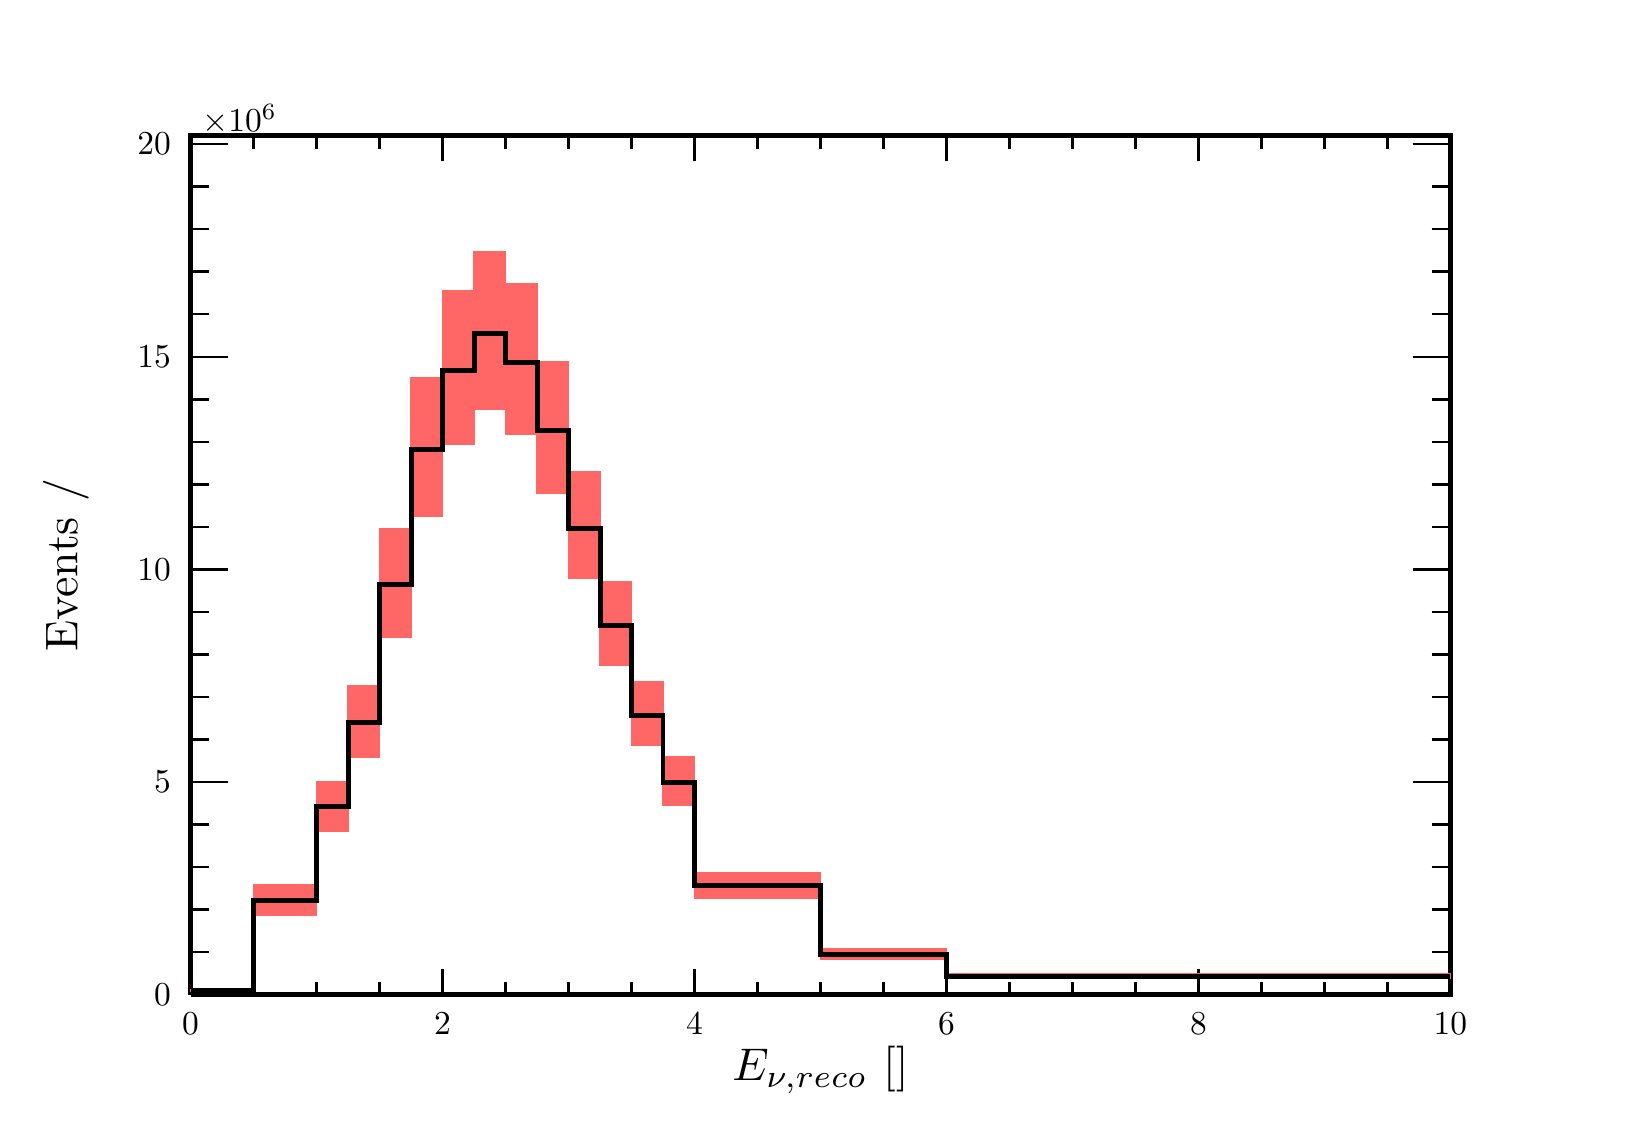
\begin{tikzpicture}
\pgfdeclareplotmark{cross} {
\pgfpathmoveto{\pgfpoint{-0.3\pgfplotmarksize}{\pgfplotmarksize}}
\pgfpathlineto{\pgfpoint{+0.3\pgfplotmarksize}{\pgfplotmarksize}}
\pgfpathlineto{\pgfpoint{+0.3\pgfplotmarksize}{0.3\pgfplotmarksize}}
\pgfpathlineto{\pgfpoint{+1\pgfplotmarksize}{0.3\pgfplotmarksize}}
\pgfpathlineto{\pgfpoint{+1\pgfplotmarksize}{-0.3\pgfplotmarksize}}
\pgfpathlineto{\pgfpoint{+0.3\pgfplotmarksize}{-0.3\pgfplotmarksize}}
\pgfpathlineto{\pgfpoint{+0.3\pgfplotmarksize}{-1.\pgfplotmarksize}}
\pgfpathlineto{\pgfpoint{-0.3\pgfplotmarksize}{-1.\pgfplotmarksize}}
\pgfpathlineto{\pgfpoint{-0.3\pgfplotmarksize}{-0.3\pgfplotmarksize}}
\pgfpathlineto{\pgfpoint{-1.\pgfplotmarksize}{-0.3\pgfplotmarksize}}
\pgfpathlineto{\pgfpoint{-1.\pgfplotmarksize}{0.3\pgfplotmarksize}}
\pgfpathlineto{\pgfpoint{-0.3\pgfplotmarksize}{0.3\pgfplotmarksize}}
\pgfpathclose
\pgfusepathqstroke
}
\pgfdeclareplotmark{cross*} {
\pgfpathmoveto{\pgfpoint{-0.3\pgfplotmarksize}{\pgfplotmarksize}}
\pgfpathlineto{\pgfpoint{+0.3\pgfplotmarksize}{\pgfplotmarksize}}
\pgfpathlineto{\pgfpoint{+0.3\pgfplotmarksize}{0.3\pgfplotmarksize}}
\pgfpathlineto{\pgfpoint{+1\pgfplotmarksize}{0.3\pgfplotmarksize}}
\pgfpathlineto{\pgfpoint{+1\pgfplotmarksize}{-0.3\pgfplotmarksize}}
\pgfpathlineto{\pgfpoint{+0.3\pgfplotmarksize}{-0.3\pgfplotmarksize}}
\pgfpathlineto{\pgfpoint{+0.3\pgfplotmarksize}{-1.\pgfplotmarksize}}
\pgfpathlineto{\pgfpoint{-0.3\pgfplotmarksize}{-1.\pgfplotmarksize}}
\pgfpathlineto{\pgfpoint{-0.3\pgfplotmarksize}{-0.3\pgfplotmarksize}}
\pgfpathlineto{\pgfpoint{-1.\pgfplotmarksize}{-0.3\pgfplotmarksize}}
\pgfpathlineto{\pgfpoint{-1.\pgfplotmarksize}{0.3\pgfplotmarksize}}
\pgfpathlineto{\pgfpoint{-0.3\pgfplotmarksize}{0.3\pgfplotmarksize}}
\pgfpathclose
\pgfusepathqfillstroke
}
\pgfdeclareplotmark{newstar} {
\pgfpathmoveto{\pgfqpoint{0pt}{\pgfplotmarksize}}
\pgfpathlineto{\pgfqpointpolar{44}{0.5\pgfplotmarksize}}
\pgfpathlineto{\pgfqpointpolar{18}{\pgfplotmarksize}}
\pgfpathlineto{\pgfqpointpolar{-20}{0.5\pgfplotmarksize}}
\pgfpathlineto{\pgfqpointpolar{-54}{\pgfplotmarksize}}
\pgfpathlineto{\pgfqpointpolar{-90}{0.5\pgfplotmarksize}}
\pgfpathlineto{\pgfqpointpolar{234}{\pgfplotmarksize}}
\pgfpathlineto{\pgfqpointpolar{198}{0.5\pgfplotmarksize}}
\pgfpathlineto{\pgfqpointpolar{162}{\pgfplotmarksize}}
\pgfpathlineto{\pgfqpointpolar{134}{0.5\pgfplotmarksize}}
\pgfpathclose
\pgfusepathqstroke
}
\pgfdeclareplotmark{newstar*} {
\pgfpathmoveto{\pgfqpoint{0pt}{\pgfplotmarksize}}
\pgfpathlineto{\pgfqpointpolar{44}{0.5\pgfplotmarksize}}
\pgfpathlineto{\pgfqpointpolar{18}{\pgfplotmarksize}}
\pgfpathlineto{\pgfqpointpolar{-20}{0.5\pgfplotmarksize}}
\pgfpathlineto{\pgfqpointpolar{-54}{\pgfplotmarksize}}
\pgfpathlineto{\pgfqpointpolar{-90}{0.5\pgfplotmarksize}}
\pgfpathlineto{\pgfqpointpolar{234}{\pgfplotmarksize}}
\pgfpathlineto{\pgfqpointpolar{198}{0.5\pgfplotmarksize}}
\pgfpathlineto{\pgfqpointpolar{162}{\pgfplotmarksize}}
\pgfpathlineto{\pgfqpointpolar{134}{0.5\pgfplotmarksize}}
\pgfpathclose
\pgfusepathqfillstroke
}
\definecolor{c}{rgb}{0.999,0.999,0.999};
\draw [color=c, fill=c] (0,0) rectangle (20,13.639);
\draw [color=c, fill=c] (2,1.3639) rectangle (18,12.2751);
\definecolor{c}{rgb}{0,0,0};
\draw [c,line width=1.8] (2,1.3639) -- (2,12.2751) -- (18,12.2751) -- (18,1.3639) -- (2,1.3639);
\definecolor{c}{rgb}{0.999,0.999,0.999};
\draw [color=c, fill=c] (2,1.3639) rectangle (18,12.2751);
\definecolor{c}{rgb}{0,0,0};
\draw [c,line width=1.8] (2,1.3639) -- (2,12.2751) -- (18,12.2751) -- (18,1.3639) -- (2,1.3639);
\draw [c,line width=1.8] (2,1.41404) -- (2.8,1.41404) -- (2.8,2.55873) -- (3.6,2.55873) -- (3.6,3.75039) -- (4,3.75039) -- (4,4.82314) -- (4.4,4.82314) -- (4.4,6.57373) -- (4.8,6.57373) -- (4.8,8.28708) -- (5.2,8.28708) -- (5.2,9.29376) --
 (5.6,9.29376) -- (5.6,9.75711) -- (6,9.75711) -- (6,9.39589) -- (6.4,9.39589) -- (6.4,8.52387) -- (6.8,8.52387) -- (6.8,7.29096) -- (7.2,7.29096) -- (7.2,6.04917) -- (7.6,6.04917) -- (7.6,4.91319) -- (8,4.91319) -- (8,4.06482) -- (8.4,4.06482) --
 (8.4,2.74593) -- (10,2.74593) -- (10,1.87667) -- (11.6,1.87667) -- (11.6,1.59709) -- (18,1.59709);
\draw [c,line width=0.9] (2,1.3639) -- (18,1.3639);
\draw [c,line width=0.9] (2,1.69123) -- (2,1.3639);
\draw [c,line width=0.9] (2.8,1.52756) -- (2.8,1.3639);
\draw [c,line width=0.9] (3.6,1.52756) -- (3.6,1.3639);
\draw [c,line width=0.9] (4.4,1.52756) -- (4.4,1.3639);
\draw [c,line width=0.9] (5.2,1.69123) -- (5.2,1.3639);
\draw [c,line width=0.9] (6,1.52756) -- (6,1.3639);
\draw [c,line width=0.9] (6.8,1.52756) -- (6.8,1.3639);
\draw [c,line width=0.9] (7.6,1.52756) -- (7.6,1.3639);
\draw [c,line width=0.9] (8.4,1.69123) -- (8.4,1.3639);
\draw [c,line width=0.9] (9.2,1.52756) -- (9.2,1.3639);
\draw [c,line width=0.9] (10,1.52756) -- (10,1.3639);
\draw [c,line width=0.9] (10.8,1.52756) -- (10.8,1.3639);
\draw [c,line width=0.9] (11.6,1.69123) -- (11.6,1.3639);
\draw [c,line width=0.9] (12.4,1.52756) -- (12.4,1.3639);
\draw [c,line width=0.9] (13.2,1.52756) -- (13.2,1.3639);
\draw [c,line width=0.9] (14,1.52756) -- (14,1.3639);
\draw [c,line width=0.9] (14.8,1.69123) -- (14.8,1.3639);
\draw [c,line width=0.9] (15.6,1.52756) -- (15.6,1.3639);
\draw [c,line width=0.9] (16.4,1.52756) -- (16.4,1.3639);
\draw [c,line width=0.9] (17.2,1.52756) -- (17.2,1.3639);
\draw [c,line width=0.9] (18,1.69123) -- (18,1.3639);
\draw [anchor=base] (2,0.859255) node[scale=1.20912, color=c, rotate=0]{0};
\draw [anchor=base] (5.2,0.859255) node[scale=1.20912, color=c, rotate=0]{2};
\draw [anchor=base] (8.4,0.859255) node[scale=1.20912, color=c, rotate=0]{4};
\draw [anchor=base] (11.6,0.859255) node[scale=1.20912, color=c, rotate=0]{6};
\draw [anchor=base] (14.8,0.859255) node[scale=1.20912, color=c, rotate=0]{8};
\draw [anchor=base] (18,0.859255) node[scale=1.20912, color=c, rotate=0]{10};
\draw (10,0.403714) node[scale=1.65459, color=c, rotate=0]{$E_{\nu, \text{reco}}$ [\si{\GeV}]};
\draw [c,line width=0.9] (2,12.2751) -- (18,12.2751);
\draw [c,line width=0.9] (2,11.9477) -- (2,12.2751);
\draw [c,line width=0.9] (2.8,12.1114) -- (2.8,12.2751);
\draw [c,line width=0.9] (3.6,12.1114) -- (3.6,12.2751);
\draw [c,line width=0.9] (4.4,12.1114) -- (4.4,12.2751);
\draw [c,line width=0.9] (5.2,11.9477) -- (5.2,12.2751);
\draw [c,line width=0.9] (6,12.1114) -- (6,12.2751);
\draw [c,line width=0.9] (6.8,12.1114) -- (6.8,12.2751);
\draw [c,line width=0.9] (7.6,12.1114) -- (7.6,12.2751);
\draw [c,line width=0.9] (8.4,11.9477) -- (8.4,12.2751);
\draw [c,line width=0.9] (9.2,12.1114) -- (9.2,12.2751);
\draw [c,line width=0.9] (10,12.1114) -- (10,12.2751);
\draw [c,line width=0.9] (10.8,12.1114) -- (10.8,12.2751);
\draw [c,line width=0.9] (11.6,11.9477) -- (11.6,12.2751);
\draw [c,line width=0.9] (12.4,12.1114) -- (12.4,12.2751);
\draw [c,line width=0.9] (13.2,12.1114) -- (13.2,12.2751);
\draw [c,line width=0.9] (14,12.1114) -- (14,12.2751);
\draw [c,line width=0.9] (14.8,11.9477) -- (14.8,12.2751);
\draw [c,line width=0.9] (15.6,12.1114) -- (15.6,12.2751);
\draw [c,line width=0.9] (16.4,12.1114) -- (16.4,12.2751);
\draw [c,line width=0.9] (17.2,12.1114) -- (17.2,12.2751);
\draw [c,line width=0.9] (18,11.9477) -- (18,12.2751);
\draw [c,line width=0.9] (2,1.3639) -- (2,12.2751);
\draw [c,line width=0.9] (2.48,1.3639) -- (2,1.3639);
\draw [c,line width=0.9] (2.24,1.90408) -- (2,1.90408);
\draw [c,line width=0.9] (2.24,2.44427) -- (2,2.44427);
\draw [c,line width=0.9] (2.24,2.98445) -- (2,2.98445);
\draw [c,line width=0.9] (2.24,3.52464) -- (2,3.52464);
\draw [c,line width=0.9] (2.48,4.06482) -- (2,4.06482);
\draw [c,line width=0.9] (2.24,4.60501) -- (2,4.60501);
\draw [c,line width=0.9] (2.24,5.14519) -- (2,5.14519);
\draw [c,line width=0.9] (2.24,5.68538) -- (2,5.68538);
\draw [c,line width=0.9] (2.24,6.22556) -- (2,6.22556);
\draw [c,line width=0.9] (2.48,6.76575) -- (2,6.76575);
\draw [c,line width=0.9] (2.24,7.30593) -- (2,7.30593);
\draw [c,line width=0.9] (2.24,7.84612) -- (2,7.84612);
\draw [c,line width=0.9] (2.24,8.3863) -- (2,8.3863);
\draw [c,line width=0.9] (2.24,8.92649) -- (2,8.92649);
\draw [c,line width=0.9] (2.48,9.46667) -- (2,9.46667);
\draw [c,line width=0.9] (2.24,10.0069) -- (2,10.0069);
\draw [c,line width=0.9] (2.24,10.547) -- (2,10.547);
\draw [c,line width=0.9] (2.24,11.0872) -- (2,11.0872);
\draw [c,line width=0.9] (2.24,11.6274) -- (2,11.6274);
\draw [c,line width=0.9] (2.48,12.1676) -- (2,12.1676);
\draw [c,line width=0.9] (2.48,12.1676) -- (2,12.1676);
\draw [anchor= east] (1.9,1.3639) node[scale=1.20912, color=c, rotate=0]{0};
\draw [anchor= east] (1.9,4.06482) node[scale=1.20912, color=c, rotate=0]{5};
\draw [anchor= east] (1.9,6.76575) node[scale=1.20912, color=c, rotate=0]{10};
\draw [anchor= east] (1.9,9.46667) node[scale=1.20912, color=c, rotate=0]{15};
\draw [anchor= east] (1.9,12.1676) node[scale=1.20912, color=c, rotate=0]{20};
\draw [anchor=base west] (2,12.3296) node[scale=1.20912, color=c, rotate=0]{$\times10^{6}$};
\draw (0.416,6.81948) node[scale=1.65459, color=c, rotate=90]{Events / \si{\GeV}};
\draw [c,line width=0.9] (18,1.3639) -- (18,12.2751);
\draw [c,line width=0.9] (17.52,1.3639) -- (18,1.3639);
\draw [c,line width=0.9] (17.76,1.90408) -- (18,1.90408);
\draw [c,line width=0.9] (17.76,2.44427) -- (18,2.44427);
\draw [c,line width=0.9] (17.76,2.98445) -- (18,2.98445);
\draw [c,line width=0.9] (17.76,3.52464) -- (18,3.52464);
\draw [c,line width=0.9] (17.52,4.06482) -- (18,4.06482);
\draw [c,line width=0.9] (17.76,4.60501) -- (18,4.60501);
\draw [c,line width=0.9] (17.76,5.14519) -- (18,5.14519);
\draw [c,line width=0.9] (17.76,5.68538) -- (18,5.68538);
\draw [c,line width=0.9] (17.76,6.22556) -- (18,6.22556);
\draw [c,line width=0.9] (17.52,6.76575) -- (18,6.76575);
\draw [c,line width=0.9] (17.76,7.30593) -- (18,7.30593);
\draw [c,line width=0.9] (17.76,7.84612) -- (18,7.84612);
\draw [c,line width=0.9] (17.76,8.3863) -- (18,8.3863);
\draw [c,line width=0.9] (17.76,8.92649) -- (18,8.92649);
\draw [c,line width=0.9] (17.52,9.46667) -- (18,9.46667);
\draw [c,line width=0.9] (17.76,10.0069) -- (18,10.0069);
\draw [c,line width=0.9] (17.76,10.547) -- (18,10.547);
\draw [c,line width=0.9] (17.76,11.0872) -- (18,11.0872);
\draw [c,line width=0.9] (17.76,11.6274) -- (18,11.6274);
\draw [c,line width=0.9] (17.52,12.1676) -- (18,12.1676);
\draw [c,line width=0.9] (17.52,12.1676) -- (18,12.1676);
\definecolor{c}{rgb}{1,0.4,0.4};
\draw [color=c, fill=c] (2,1.40191) rectangle (2.8,1.42724);
\draw [color=c, fill=c] (2.8,2.37459) rectangle (3.6,2.75935);
\draw [color=c, fill=c] (3.6,3.44297) rectangle (4,4.07616);
\draw [color=c, fill=c] (4,4.37496) rectangle (4.4,5.29674);
\draw [color=c, fill=c] (4.4,5.90504) rectangle (4.8,7.28627);
\draw [color=c, fill=c] (4.8,7.43852) rectangle (5.2,9.19798);
\draw [color=c, fill=c] (5.2,8.35719) rectangle (5.6,10.3065);
\draw [color=c, fill=c] (5.6,8.79266) rectangle (6,10.8084);
\draw [color=c, fill=c] (6,8.48593) rectangle (6.4,10.3952);
\draw [color=c, fill=c] (6.4,7.73428) rectangle (6.8,9.39958);
\draw [color=c, fill=c] (6.8,6.64608) rectangle (7.2,8.0101);
\draw [color=c, fill=c] (7.2,5.54659) rectangle (7.6,6.61171);
\draw [color=c, fill=c] (7.6,4.53405) rectangle (8,5.33873);
\draw [color=c, fill=c] (8,3.77119) rectangle (8.4,4.39406);
\draw [color=c, fill=c] (8.4,2.5868) rectangle (10,2.9214);
\draw [color=c, fill=c] (10,1.81411) rectangle (11.6,1.94488);
\draw [color=c, fill=c] (11.6,1.56714) rectangle (18,1.62917);
\definecolor{c}{rgb}{0,0,0};
\draw [c,line width=1.8] (2,1.41404) -- (2.8,1.41404) -- (2.8,2.55873) -- (3.6,2.55873) -- (3.6,3.75039) -- (4,3.75039) -- (4,4.82314) -- (4.4,4.82314) -- (4.4,6.57373) -- (4.8,6.57373) -- (4.8,8.28708) -- (5.2,8.28708) -- (5.2,9.29376) --
 (5.6,9.29376) -- (5.6,9.75711) -- (6,9.75711) -- (6,9.39589) -- (6.4,9.39589) -- (6.4,8.52387) -- (6.8,8.52387) -- (6.8,7.29096) -- (7.2,7.29096) -- (7.2,6.04917) -- (7.6,6.04917) -- (7.6,4.91319) -- (8,4.91319) -- (8,4.06482) -- (8.4,4.06482) --
 (8.4,2.74593) -- (10,2.74593) -- (10,1.87667) -- (11.6,1.87667) -- (11.6,1.59709) -- (18,1.59709);
\end{tikzpicture}
	
		\end{adjustbox}
	\end{minipage}
	\caption[One-dimensional DUNE ND event rates used in the long-baseline analysis with $\pm1\sigma$ systematic error band. The full MC statistics are used for these plots (with a scaling factor) with no fluctuations so the statistical uncertainty is not shown.]{One-dimensional DUNE ND event rates used in the long-baseline. The red band indicates the $\pm1\sigma$ systematic error band. Left: Event rate with the beam in FHC mode. Right: Event rate with the beam in RHC mode.}
	\label{fig:ndEventRatesWithError}
\end{figure}


In these fits Gaussian penalty terms on \thetai{12}, \deltami{21} and $\rho$ are applied (since DUNE will not be able to constrain these parameters).
The width and central values of these penalty terms are taken from the NuFit 4.0 global fit~\cite{nufit4}.
A penalty term on \thetai{13} may also be included.
However in the studies included in this chapter, it is not.
DUNE will eventually be able to constrain \thetai{13} with a similar precision to existing reactor experiments. 
However, this is expected to take around 15 years of running~\cite{tdrVol2}.
The other oscillation parameters, \ssthetai{23}, \deltami{32} and \dcp are allowed to vary freely.

In a typical oscillation analysis the compatibility of a particular set of oscillation parameters is evaluated using a negative log-likelihood ratio,
In the high statistics limit for Poisson-distributed data, this log-likelihood ratio converges to a $\chi^{2}$ and is given by~\cite{pdg2018}:
\begin{align}
	\chi^{2} &= -2 \log \mathcal{L} \\
	& = 2 \sum_{i}^{N_{\text{bins}}} \left[ M_{i} - D_{i} + D_{i} \ln \left( \frac{D_{i}}{M_{i}} \right) \right]
\end{align}
where $M_{i}$ and $D_{i}$ are the Monte Carlo expectation and observed count for the $i$th histogram bin respectively.

The $M_{i}$ for oscillated FD predictions are generated using simulated events where both the true and reconstructed properties of the neutrino interaction are known.
These are then used to fill 2D histograms (with the second axis being the true neutrino energy) for each oscillation channel ($\nu_{\alpha} \rightarrow \nu_{\beta}$).
These are then reweighted by the oscillation probability as a function of true energy, $P_{\alpha\beta}(E)$, to give the result
\begin{equation}
	M_{i} = \sum_{\alpha}^{e, \mu} \sum_{\beta}^{e, \mu, \tau} \sum_{j} P_{\alpha\beta}(E_{j}) M_{ij}^{\alpha\beta} \, .	
\end{equation}

The systematic parameters detailed in \citesec{sec:dune_lbl:systs} are included as nuisance parameters in the fit. 
These can have an arbitrary effect on the MC predictions and can affect different channels in different ways.
These parameters are profiled over in order to minimise the value of \chisquare and are prevented from moving too far from their expected values by gaussian penalty terms.
These penalty terms reflect our prior knowledge of what constitutes a likely variation in a given parameter.
To determine $M_{i}$ for a given set of systematic parameters, $M_{ij}^{\alpha\beta}$ is evaluated for each systematic parameter at $\pm1,2,3\sigma$ and an interpolation is used.

Including the systematic parameters and the covariance matrix gives $\chi^{2}$ for a given set of oscillation parameters, $\bm{\theta}$, and nuisance parameters, $\vb{x}$, as
\begin{align}
	\chi^{2} \left( \bm{\theta}, \vb{x} \right) &= -2 \log \mathcal{L} \left( \bm{\theta}, \vb{x} \right) \\
	&= 2 \sum_{i}^{N_{\text{bins}}} \left[ M_{i} (\bm{\theta}, \vb{x}) - D_{i} + D_{i} \ln \left( \frac{D_{i}}{M_{i}(\bm{\theta}, \vb{x})} \right) \right] + \sum_{j}^{N_{\text{systs}}} \left[ \frac{\Delta x_{j}}{\sigma_{j}} \right]^{2} \nonumber \\
	&+ \sum_{k}^{N^{\text{ND}}_{\text{bins}}} \sum_{l}^{ N_{\text{bins}}^{\text{ND}} } \left(  M_{k} (\vb{x}) - D_{k} \right) V_{kl}^{-1} \left( M_{l}(\vb{x}) - D_{l} \right) \, ,
\end{align}
where $M_{i}(\bm{\theta}, \vb{x})$ is the Monte Carlo expectation for a given set of $\bm{\theta}$ and $\vb{x}$ for the $i$th bin. 
$V_{kl}$ is the ND covariance matrix discussed in \citesec{sec:dune_lbl:systs:det}.
$\Delta x_{j}$ is the difference between the nominal and current value of the $j$th nuisance parameter and $\sigma_{j}$ is the prior uncertainty on said parameter.
The best fit values for the $\bm{\theta}$ and $\vb{x}$ occur at the minimum value of $\chi^{2}$.

The $D_{i}$ may or may not have Poisson fluctuations added depending on the type of study in question.
The fits utilised in this chapter are all Asimov studies~\cite{asimov}.
In these fits, the fake dataset is the same as the nominal Monte Carlo up to some scaling exposure and there are no throws of oscillation parameters, the systematic parameters or the bin statistics.
These fits provide the median sensitivity without the need to run many toy fits with statistical and systematic fluctuations.

In order to avoid reporting a false minimum $\chi^{2}$ as the true one, each fit is repeated at multiple sets of oscillation parameters. 
The values of \dcp tested are $-\pi$, $-\pi/2$, 0 and $\pi/2$. 
Additionally, both neutrino mass hierarchies are tested along with both octants of \thetai{23}.
From these, the fit which provides the lowest \chisquare is selected as the best fit point.

\subsection{Constraints on systematic parameters}

\citefig{fig:systConstraints} shows the systematics used in the DUNE long-baseline analysis.
For each parameter, the ratio of the post-fit to pre-fit uncertainties is shown for a 15 year staged exposure (\SI{1104}{\kilo\tonne\mega\watt\year}).
The constraints with just the FD are shown in red, while the green lines show the constraints with both the ND and FD samples.
The constraints are divided up depending on if they fall into the category of detector, flux or cross-section uncertainties.

\begin{figure}[h]
	\centering
	\includegraphics[width=.8\linewidth]{files/figures/dune_lbl/constraintsWithLines}
	\caption[DUNE systematic constraints with and without a near detector constraint]{Ratio of post-fit to pre-fit systematic constraints for a 15 year staged exposure. The constraints with (green) and without a ND constraint (red) are shown. The systematics are separated by category. Taken from~\cite{Abi:2020qib}.}
	\label{fig:systConstraints}
\end{figure}

For the detector systematics, one can see that the vast majority are not well constrained, either by the FD samples or with the additional ND samples.
Given that most of these parameters affect particles in the FD only it is reassuring to see that the addition of ND samples does not increase the constraints on most of these parameters.

The flux parameters are labelled as ``flux~$i$'', representing the $i\text{th}$ principal component of the matrix described in \citesec{sec:dune_lbl:systs:flux}.
One can see that most of the flux components are not constrained at all by the FD samples but with the inclusion of the ND, all become noticeably more constrained.

The level at which various cross-section parameters are constrained shows significant variation. 
For the most part (similar to the flux systematics), these parameters are not well constrained by the FD only, showing the utility of the ND.


\subsection{Mass hierarchy}
\label{sec:dune_lbl:sensitivities:mh}

DUNE's sensitivity to the neutrino mass hierarchy is measured using the statistic $\Delta \chisquare = \chi^{2}_{\text{B}} - \chi^{2}_{\text{A}}$, where $A$ and $B$ are two possible hypotheses.
This provides a measure of how well the data can exclude hypothesis $B$ in favour of $A$.
In the case of the neutrino mass hierarchy, the relevant question is to what level DUNE can exclude the inverted hierarchy in favour of the normal hierarchy (in the case of true normal hierarchy), $\chi^{2}_{\text{IH}} - \chi^{2}_{\text{NH}}$, and vice versa if the hierarchy is truly inverted.

This is repeated for various true values of \dcp, for both hierarchies in \citefig{fig:mhSens}.
For each \dcp point, $\Delta \chisquare$ is calculated by first calculating $\chi^{2}_{\text{true}}$ (where this can be either the normal or inverted hierarchy) and then calculating the \chisquare value for the same value of \dcp but with the hierarchy fixed to the incorrect value.
The square root of $\Delta \chisquare$ is then taken to provide a crude significance.

\begin{figure}[h]
	\begin{adjustbox}{max totalsize=.6\linewidth, center}
		\input{files/figures/dune_lbl/mh_sens_both}
	\end{adjustbox}
	\caption[DUNE sensitivity to the neutrino mass hierarchy as a function of true \dcp.]{DUNE sensitivities to the neutrino mass hierarchy as a function of true \dcp for a 7 year staged exposure. The black line shows the statistics-only case. The blue line shows the case where only the detector systematics are used. The red line shows the case where all systematics are used. Solid lines show the case for true normal mass hierarchy while dashed lines show the case for true inverted mass hierarchy. The two horizontal dashed lines are at $\sqrt{\Delta\chi^{2}} = 3, 5$ and represent important milestones in determining the mass hierarchy.}
	\label{fig:mhSens}
\end{figure}

\citefig{fig:mhSens} shows the results of this in the statistics-only case (for 7 years of staged running - equivalent to an exposure of \SI{336}{\kilo\tonne\mega\watt\year}), with just the detector systematics and also all the systematics included.
It is immediately apparent that DUNE will be highly sensitive to the neutrino mass hierarchy, surpassing the common particle physics threshold of $\sqrt{\Delta \chisquare} = 5$ at all values of \dcp and for both true hierarchies.
One can see that the addition of detector systematics reduces the sensitivity somewhat, with remaining systematics reducing it further.
However, it is clear that, even with a fairly substantial increase in systematic uncertainties, DUNE will still be able to quickly resolve the neutrino mass hierarchy.
This excellent ability to resolve the mass hierarchy stems from DUNE's long baseline which increases the size of matter effects on the oscillations. 
Since these matter effects are dependent on the true neutrino mass hierarchy, a longer baseline allows a quicker determination of the true mass hierarchy.

\citefig{fig:mhSensExp} illustrates just how quickly DUNE will be able to resolve the mass hierarchy.
\citefig{fig:mhSensExp} shows the value of $\sqrt{\Delta\chisquare}$ in the case of true normal neutrino mass hierarchy and $\dcpTrue = \pi/2$ as a function of far detector exposure. 
Looking at \citefig{fig:mhSens}, one can see that this is the value at which DUNE is least sensitive to the mass hierarchy and thus a worst-case scenario for DUNE to make this measurement.
Therefore, regardless of the choice of \dcp, one can see that DUNE would pass the $\sqrt{\Delta\chisquare}=3$ threshold after an exposure of roughly \SI{22}{\kilo\tonne\mega\watt\year}.
Similarly, the $\sqrt{\Delta\chisquare}=5$ threshold is passed after an exposure of roughly \SI{78}{\kilo\tonne\mega\watt\year}.
Given that the full DUNE FD is expected to have a fiducial mass of \SI{40}{\kilo\tonne} and an initial beam power of \SI{1.2}{\mega\watt}, the required exposure for definitive discovery of the mass hierachy could be accumulated in less than 2 years.

\begin{figure}[h]
	\begin{adjustbox}{max totalsize=.6\linewidth, center}
		\begin{tikzpicture}
\pgfdeclareplotmark{cross} {
\pgfpathmoveto{\pgfpoint{-0.3\pgfplotmarksize}{\pgfplotmarksize}}
\pgfpathlineto{\pgfpoint{+0.3\pgfplotmarksize}{\pgfplotmarksize}}
\pgfpathlineto{\pgfpoint{+0.3\pgfplotmarksize}{0.3\pgfplotmarksize}}
\pgfpathlineto{\pgfpoint{+1\pgfplotmarksize}{0.3\pgfplotmarksize}}
\pgfpathlineto{\pgfpoint{+1\pgfplotmarksize}{-0.3\pgfplotmarksize}}
\pgfpathlineto{\pgfpoint{+0.3\pgfplotmarksize}{-0.3\pgfplotmarksize}}
\pgfpathlineto{\pgfpoint{+0.3\pgfplotmarksize}{-1.\pgfplotmarksize}}
\pgfpathlineto{\pgfpoint{-0.3\pgfplotmarksize}{-1.\pgfplotmarksize}}
\pgfpathlineto{\pgfpoint{-0.3\pgfplotmarksize}{-0.3\pgfplotmarksize}}
\pgfpathlineto{\pgfpoint{-1.\pgfplotmarksize}{-0.3\pgfplotmarksize}}
\pgfpathlineto{\pgfpoint{-1.\pgfplotmarksize}{0.3\pgfplotmarksize}}
\pgfpathlineto{\pgfpoint{-0.3\pgfplotmarksize}{0.3\pgfplotmarksize}}
\pgfpathclose
\pgfusepathqstroke
}
\pgfdeclareplotmark{cross*} {
\pgfpathmoveto{\pgfpoint{-0.3\pgfplotmarksize}{\pgfplotmarksize}}
\pgfpathlineto{\pgfpoint{+0.3\pgfplotmarksize}{\pgfplotmarksize}}
\pgfpathlineto{\pgfpoint{+0.3\pgfplotmarksize}{0.3\pgfplotmarksize}}
\pgfpathlineto{\pgfpoint{+1\pgfplotmarksize}{0.3\pgfplotmarksize}}
\pgfpathlineto{\pgfpoint{+1\pgfplotmarksize}{-0.3\pgfplotmarksize}}
\pgfpathlineto{\pgfpoint{+0.3\pgfplotmarksize}{-0.3\pgfplotmarksize}}
\pgfpathlineto{\pgfpoint{+0.3\pgfplotmarksize}{-1.\pgfplotmarksize}}
\pgfpathlineto{\pgfpoint{-0.3\pgfplotmarksize}{-1.\pgfplotmarksize}}
\pgfpathlineto{\pgfpoint{-0.3\pgfplotmarksize}{-0.3\pgfplotmarksize}}
\pgfpathlineto{\pgfpoint{-1.\pgfplotmarksize}{-0.3\pgfplotmarksize}}
\pgfpathlineto{\pgfpoint{-1.\pgfplotmarksize}{0.3\pgfplotmarksize}}
\pgfpathlineto{\pgfpoint{-0.3\pgfplotmarksize}{0.3\pgfplotmarksize}}
\pgfpathclose
\pgfusepathqfillstroke
}
\pgfdeclareplotmark{newstar} {
\pgfpathmoveto{\pgfqpoint{0pt}{\pgfplotmarksize}}
\pgfpathlineto{\pgfqpointpolar{44}{0.5\pgfplotmarksize}}
\pgfpathlineto{\pgfqpointpolar{18}{\pgfplotmarksize}}
\pgfpathlineto{\pgfqpointpolar{-20}{0.5\pgfplotmarksize}}
\pgfpathlineto{\pgfqpointpolar{-54}{\pgfplotmarksize}}
\pgfpathlineto{\pgfqpointpolar{-90}{0.5\pgfplotmarksize}}
\pgfpathlineto{\pgfqpointpolar{234}{\pgfplotmarksize}}
\pgfpathlineto{\pgfqpointpolar{198}{0.5\pgfplotmarksize}}
\pgfpathlineto{\pgfqpointpolar{162}{\pgfplotmarksize}}
\pgfpathlineto{\pgfqpointpolar{134}{0.5\pgfplotmarksize}}
\pgfpathclose
\pgfusepathqstroke
}
\pgfdeclareplotmark{newstar*} {
\pgfpathmoveto{\pgfqpoint{0pt}{\pgfplotmarksize}}
\pgfpathlineto{\pgfqpointpolar{44}{0.5\pgfplotmarksize}}
\pgfpathlineto{\pgfqpointpolar{18}{\pgfplotmarksize}}
\pgfpathlineto{\pgfqpointpolar{-20}{0.5\pgfplotmarksize}}
\pgfpathlineto{\pgfqpointpolar{-54}{\pgfplotmarksize}}
\pgfpathlineto{\pgfqpointpolar{-90}{0.5\pgfplotmarksize}}
\pgfpathlineto{\pgfqpointpolar{234}{\pgfplotmarksize}}
\pgfpathlineto{\pgfqpointpolar{198}{0.5\pgfplotmarksize}}
\pgfpathlineto{\pgfqpointpolar{162}{\pgfplotmarksize}}
\pgfpathlineto{\pgfqpointpolar{134}{0.5\pgfplotmarksize}}
\pgfpathclose
\pgfusepathqfillstroke
}
\definecolor{c}{rgb}{1,1,1};
\draw [color=c, fill=c] (0,0) rectangle (20,13.639);
\draw [color=c, fill=c] (3.23782,1.7765) rectangle (18.5387,12.2923);
\definecolor{c}{rgb}{0,0,0};
\draw [c,line width=0.9] (3.23782,1.7765) -- (3.23782,12.2923) -- (18.5387,12.2923) -- (18.5387,1.7765) -- (3.23782,1.7765);
\definecolor{c}{rgb}{1,1,1};
\draw [color=c, fill=c] (3.23782,1.7765) rectangle (18.5387,12.2923);
\definecolor{c}{rgb}{0,0,0};
\draw [c,line width=0.9] (3.23782,1.7765) -- (3.23782,12.2923) -- (18.5387,12.2923) -- (18.5387,1.7765) -- (3.23782,1.7765);
\draw [c,line width=0.9] (3.23782,1.7765) -- (18.5387,1.7765);
\draw [c,line width=0.9] (4.81227,2.08954) -- (4.81227,1.7765);
\draw [c,line width=0.9] (5.33483,1.93302) -- (5.33483,1.7765);
\draw [c,line width=0.9] (5.85738,1.93302) -- (5.85738,1.7765);
\draw [c,line width=0.9] (6.37993,1.93302) -- (6.37993,1.7765);
\draw [c,line width=0.9] (6.90248,2.08954) -- (6.90248,1.7765);
\draw [c,line width=0.9] (7.42504,1.93302) -- (7.42504,1.7765);
\draw [c,line width=0.9] (7.94759,1.93302) -- (7.94759,1.7765);
\draw [c,line width=0.9] (8.47014,1.93302) -- (8.47014,1.7765);
\draw [c,line width=0.9] (8.99269,2.08954) -- (8.99269,1.7765);
\draw [c,line width=0.9] (9.51525,1.93302) -- (9.51525,1.7765);
\draw [c,line width=0.9] (10.0378,1.93302) -- (10.0378,1.7765);
\draw [c,line width=0.9] (10.5604,1.93302) -- (10.5604,1.7765);
\draw [c,line width=0.9] (11.0829,2.08954) -- (11.0829,1.7765);
\draw [c,line width=0.9] (11.6055,1.93302) -- (11.6055,1.7765);
\draw [c,line width=0.9] (12.128,1.93302) -- (12.128,1.7765);
\draw [c,line width=0.9] (12.6506,1.93302) -- (12.6506,1.7765);
\draw [c,line width=0.9] (13.1731,2.08954) -- (13.1731,1.7765);
\draw [c,line width=0.9] (13.6957,1.93302) -- (13.6957,1.7765);
\draw [c,line width=0.9] (14.2182,1.93302) -- (14.2182,1.7765);
\draw [c,line width=0.9] (14.7408,1.93302) -- (14.7408,1.7765);
\draw [c,line width=0.9] (15.2633,2.08954) -- (15.2633,1.7765);
\draw [c,line width=0.9] (15.7859,1.93302) -- (15.7859,1.7765);
\draw [c,line width=0.9] (16.3084,1.93302) -- (16.3084,1.7765);
\draw [c,line width=0.9] (16.831,1.93302) -- (16.831,1.7765);
\draw [c,line width=0.9] (17.3535,2.08954) -- (17.3535,1.7765);
\draw [c,line width=0.9] (4.81227,2.08954) -- (4.81227,1.7765);
\draw [c,line width=0.9] (4.28972,1.93302) -- (4.28972,1.7765);
\draw [c,line width=0.9] (3.76717,1.93302) -- (3.76717,1.7765);
\draw [c,line width=0.9] (3.24462,1.93302) -- (3.24462,1.7765);
\draw [c,line width=0.9] (17.3535,2.08954) -- (17.3535,1.7765);
\draw [c,line width=0.9] (17.8761,1.93302) -- (17.8761,1.7765);
\draw [c,line width=0.9] (18.3986,1.93302) -- (18.3986,1.7765);
\draw [anchor=base] (4.81227,1.16275) node[scale=1.52731, color=c, rotate=0]{20};
\draw [anchor=base] (6.90248,1.16275) node[scale=1.52731, color=c, rotate=0]{40};
\draw [anchor=base] (8.99269,1.16275) node[scale=1.52731, color=c, rotate=0]{60};
\draw [anchor=base] (11.0829,1.16275) node[scale=1.52731, color=c, rotate=0]{80};
\draw [anchor=base] (13.1731,1.16275) node[scale=1.52731, color=c, rotate=0]{100};
\draw [anchor=base] (15.2633,1.16275) node[scale=1.52731, color=c, rotate=0]{120};
\draw [anchor=base] (17.3535,1.16275) node[scale=1.52731, color=c, rotate=0]{140};
\draw [anchor= east] (18.5387,0.576275) node[scale=1.52731, color=c, rotate=0]{Exposure [\si{\kilo\tonne\mega\watt\year}] };
\draw [c,line width=0.9] (3.23782,12.2923) -- (18.5387,12.2923);
\draw [c,line width=0.9] (4.81227,11.9792) -- (4.81227,12.2923);
\draw [c,line width=0.9] (5.33483,12.1357) -- (5.33483,12.2923);
\draw [c,line width=0.9] (5.85738,12.1357) -- (5.85738,12.2923);
\draw [c,line width=0.9] (6.37993,12.1357) -- (6.37993,12.2923);
\draw [c,line width=0.9] (6.90248,11.9792) -- (6.90248,12.2923);
\draw [c,line width=0.9] (7.42504,12.1357) -- (7.42504,12.2923);
\draw [c,line width=0.9] (7.94759,12.1357) -- (7.94759,12.2923);
\draw [c,line width=0.9] (8.47014,12.1357) -- (8.47014,12.2923);
\draw [c,line width=0.9] (8.99269,11.9792) -- (8.99269,12.2923);
\draw [c,line width=0.9] (9.51525,12.1357) -- (9.51525,12.2923);
\draw [c,line width=0.9] (10.0378,12.1357) -- (10.0378,12.2923);
\draw [c,line width=0.9] (10.5604,12.1357) -- (10.5604,12.2923);
\draw [c,line width=0.9] (11.0829,11.9792) -- (11.0829,12.2923);
\draw [c,line width=0.9] (11.6055,12.1357) -- (11.6055,12.2923);
\draw [c,line width=0.9] (12.128,12.1357) -- (12.128,12.2923);
\draw [c,line width=0.9] (12.6506,12.1357) -- (12.6506,12.2923);
\draw [c,line width=0.9] (13.1731,11.9792) -- (13.1731,12.2923);
\draw [c,line width=0.9] (13.6957,12.1357) -- (13.6957,12.2923);
\draw [c,line width=0.9] (14.2182,12.1357) -- (14.2182,12.2923);
\draw [c,line width=0.9] (14.7408,12.1357) -- (14.7408,12.2923);
\draw [c,line width=0.9] (15.2633,11.9792) -- (15.2633,12.2923);
\draw [c,line width=0.9] (15.7859,12.1357) -- (15.7859,12.2923);
\draw [c,line width=0.9] (16.3084,12.1357) -- (16.3084,12.2923);
\draw [c,line width=0.9] (16.831,12.1357) -- (16.831,12.2923);
\draw [c,line width=0.9] (17.3535,11.9792) -- (17.3535,12.2923);
\draw [c,line width=0.9] (4.81227,11.9792) -- (4.81227,12.2923);
\draw [c,line width=0.9] (4.28972,12.1357) -- (4.28972,12.2923);
\draw [c,line width=0.9] (3.76717,12.1357) -- (3.76717,12.2923);
\draw [c,line width=0.9] (3.24462,12.1357) -- (3.24462,12.2923);
\draw [c,line width=0.9] (17.3535,11.9792) -- (17.3535,12.2923);
\draw [c,line width=0.9] (17.8761,12.1357) -- (17.8761,12.2923);
\draw [c,line width=0.9] (18.3986,12.1357) -- (18.3986,12.2923);
\draw [c,line width=0.9] (3.23782,1.7765) -- (3.23782,12.2923);
\draw [c,line width=0.9] (3.70043,1.7765) -- (3.23782,1.7765);
\draw [c,line width=0.9] (3.46912,2.07695) -- (3.23782,2.07695);
\draw [c,line width=0.9] (3.46912,2.3774) -- (3.23782,2.3774);
\draw [c,line width=0.9] (3.46912,2.67786) -- (3.23782,2.67786);
\draw [c,line width=0.9] (3.46912,2.97831) -- (3.23782,2.97831);
\draw [c,line width=0.9] (3.70043,3.27876) -- (3.23782,3.27876);
\draw [c,line width=0.9] (3.46912,3.57921) -- (3.23782,3.57921);
\draw [c,line width=0.9] (3.46912,3.87966) -- (3.23782,3.87966);
\draw [c,line width=0.9] (3.46912,4.18011) -- (3.23782,4.18011);
\draw [c,line width=0.9] (3.46912,4.48056) -- (3.23782,4.48056);
\draw [c,line width=0.9] (3.70043,4.78101) -- (3.23782,4.78101);
\draw [c,line width=0.9] (3.46912,5.08146) -- (3.23782,5.08146);
\draw [c,line width=0.9] (3.46912,5.38191) -- (3.23782,5.38191);
\draw [c,line width=0.9] (3.46912,5.68236) -- (3.23782,5.68236);
\draw [c,line width=0.9] (3.46912,5.98281) -- (3.23782,5.98281);
\draw [c,line width=0.9] (3.70043,6.28326) -- (3.23782,6.28326);
\draw [c,line width=0.9] (3.46912,6.58371) -- (3.23782,6.58371);
\draw [c,line width=0.9] (3.46912,6.88416) -- (3.23782,6.88416);
\draw [c,line width=0.9] (3.46912,7.18461) -- (3.23782,7.18461);
\draw [c,line width=0.9] (3.46912,7.48506) -- (3.23782,7.48506);
\draw [c,line width=0.9] (3.70043,7.78551) -- (3.23782,7.78551);
\draw [c,line width=0.9] (3.46912,8.08596) -- (3.23782,8.08596);
\draw [c,line width=0.9] (3.46912,8.38641) -- (3.23782,8.38641);
\draw [c,line width=0.9] (3.46912,8.68686) -- (3.23782,8.68686);
\draw [c,line width=0.9] (3.46912,8.98731) -- (3.23782,8.98731);
\draw [c,line width=0.9] (3.70043,9.28776) -- (3.23782,9.28776);
\draw [c,line width=0.9] (3.46912,9.58821) -- (3.23782,9.58821);
\draw [c,line width=0.9] (3.46912,9.88866) -- (3.23782,9.88866);
\draw [c,line width=0.9] (3.46912,10.1891) -- (3.23782,10.1891);
\draw [c,line width=0.9] (3.46912,10.4896) -- (3.23782,10.4896);
\draw [c,line width=0.9] (3.70043,10.79) -- (3.23782,10.79);
\draw [c,line width=0.9] (3.46912,11.0905) -- (3.23782,11.0905);
\draw [c,line width=0.9] (3.46912,11.3909) -- (3.23782,11.3909);
\draw [c,line width=0.9] (3.46912,11.6914) -- (3.23782,11.6914);
\draw [c,line width=0.9] (3.46912,11.9918) -- (3.23782,11.9918);
\draw [c,line width=0.9] (3.70043,12.2923) -- (3.23782,12.2923);
\draw [anchor= east] (3.13782,1.7765) node[scale=1.52731, color=c, rotate=0]{0};
\draw [anchor= east] (3.13782,3.27876) node[scale=1.52731, color=c, rotate=0]{1};
\draw [anchor= east] (3.13782,4.78101) node[scale=1.52731, color=c, rotate=0]{2};
\draw [anchor= east] (3.13782,6.28326) node[scale=1.52731, color=c, rotate=0]{3};
\draw [anchor= east] (3.13782,7.78551) node[scale=1.52731, color=c, rotate=0]{4};
\draw [anchor= east] (3.13782,9.28776) node[scale=1.52731, color=c, rotate=0]{5};
\draw [anchor= east] (3.13782,10.79) node[scale=1.52731, color=c, rotate=0]{6};
\draw [anchor= east] (3.13782,12.2923) node[scale=1.52731, color=c, rotate=0]{7};
\draw [anchor= east] (1.47782,12.2923) node[scale=1.52731, color=c, rotate=90]{$\sqrt{ \Delta \chi^{2} }$};
\draw [c,line width=0.9] (18.5387,1.7765) -- (18.5387,12.2923);
\draw [c,line width=0.9] (18.0761,1.7765) -- (18.5387,1.7765);
\draw [c,line width=0.9] (18.3074,2.07695) -- (18.5387,2.07695);
\draw [c,line width=0.9] (18.3074,2.3774) -- (18.5387,2.3774);
\draw [c,line width=0.9] (18.3074,2.67786) -- (18.5387,2.67786);
\draw [c,line width=0.9] (18.3074,2.97831) -- (18.5387,2.97831);
\draw [c,line width=0.9] (18.0761,3.27876) -- (18.5387,3.27876);
\draw [c,line width=0.9] (18.3074,3.57921) -- (18.5387,3.57921);
\draw [c,line width=0.9] (18.3074,3.87966) -- (18.5387,3.87966);
\draw [c,line width=0.9] (18.3074,4.18011) -- (18.5387,4.18011);
\draw [c,line width=0.9] (18.3074,4.48056) -- (18.5387,4.48056);
\draw [c,line width=0.9] (18.0761,4.78101) -- (18.5387,4.78101);
\draw [c,line width=0.9] (18.3074,5.08146) -- (18.5387,5.08146);
\draw [c,line width=0.9] (18.3074,5.38191) -- (18.5387,5.38191);
\draw [c,line width=0.9] (18.3074,5.68236) -- (18.5387,5.68236);
\draw [c,line width=0.9] (18.3074,5.98281) -- (18.5387,5.98281);
\draw [c,line width=0.9] (18.0761,6.28326) -- (18.5387,6.28326);
\draw [c,line width=0.9] (18.3074,6.58371) -- (18.5387,6.58371);
\draw [c,line width=0.9] (18.3074,6.88416) -- (18.5387,6.88416);
\draw [c,line width=0.9] (18.3074,7.18461) -- (18.5387,7.18461);
\draw [c,line width=0.9] (18.3074,7.48506) -- (18.5387,7.48506);
\draw [c,line width=0.9] (18.0761,7.78551) -- (18.5387,7.78551);
\draw [c,line width=0.9] (18.3074,8.08596) -- (18.5387,8.08596);
\draw [c,line width=0.9] (18.3074,8.38641) -- (18.5387,8.38641);
\draw [c,line width=0.9] (18.3074,8.68686) -- (18.5387,8.68686);
\draw [c,line width=0.9] (18.3074,8.98731) -- (18.5387,8.98731);
\draw [c,line width=0.9] (18.0761,9.28776) -- (18.5387,9.28776);
\draw [c,line width=0.9] (18.3074,9.58821) -- (18.5387,9.58821);
\draw [c,line width=0.9] (18.3074,9.88866) -- (18.5387,9.88866);
\draw [c,line width=0.9] (18.3074,10.1891) -- (18.5387,10.1891);
\draw [c,line width=0.9] (18.3074,10.4896) -- (18.5387,10.4896);
\draw [c,line width=0.9] (18.0761,10.79) -- (18.5387,10.79);
\draw [c,line width=0.9] (18.3074,11.0905) -- (18.5387,11.0905);
\draw [c,line width=0.9] (18.3074,11.3909) -- (18.5387,11.3909);
\draw [c,line width=0.9] (18.3074,11.6914) -- (18.5387,11.6914);
\draw [c,line width=0.9] (18.3074,11.9918) -- (18.5387,11.9918);
\draw [c,line width=0.9] (18.0761,12.2923) -- (18.5387,12.2923);
\draw [c,line width=1.8] (3.24462,3.7028) -- (3.76717,4.49967) -- (4.28972,5.11044) -- (4.81227,5.62477) -- (5.33483,6.07739) -- (5.85738,6.48614) -- (6.37993,6.86157) -- (6.90248,7.21067) -- (7.42504,7.53817) -- (7.94759,7.84759) --
 (8.47014,8.14157) -- (8.99269,8.42215) -- (9.51525,8.69097) -- (10.0378,8.94936) -- (10.5604,9.1984) -- (11.0829,9.43901) -- (11.6055,9.67195) -- (12.128,9.8979) -- (12.6506,10.1174) -- (13.1731,10.331) -- (13.6957,10.539) -- (14.2182,10.742) --
 (14.7408,10.9402) -- (15.2633,11.1339) -- (15.7859,11.3235) -- (16.3084,11.509) -- (16.831,11.6909) -- (17.3535,11.8692) -- (17.8761,12.0442) -- (18.3986,12.216);
\definecolor{c}{rgb}{0,0,1};
\draw [c,line width=1.8] (3.24462,3.69876) -- (3.76717,4.49035) -- (4.28972,5.09621) -- (4.81227,5.6058) -- (5.33483,6.05384) -- (5.85738,6.45821) -- (6.37993,6.82946) -- (6.90248,7.17446) -- (7.42504,7.498) -- (7.94759,7.80335) -- (8.47014,8.09341)
 -- (8.99269,8.37029) -- (9.51525,8.63541) -- (10.0378,8.89015) -- (10.5604,9.1356) -- (11.0829,9.37247) -- (11.6055,9.60189) -- (12.128,9.82434) -- (12.6506,10.0404) -- (13.1731,10.2505) -- (13.6957,10.4553) -- (14.2182,10.6549) -- (14.7408,10.8498)
 -- (15.2633,11.0402) -- (15.7859,11.2264) -- (16.3084,11.4087) -- (16.831,11.5873) -- (17.3535,11.7624) -- (17.8761,11.9342) -- (18.3986,12.1028);
\definecolor{c}{rgb}{1,0,0};
\draw [c,line width=1.8] (3.24462,3.69813) -- (3.76717,4.4892) -- (4.28972,5.09363) -- (4.81227,5.60212) -- (5.33483,6.04902) -- (5.85738,6.45214) -- (6.37993,6.82206) -- (6.90248,7.16566) -- (7.42504,7.48775) -- (7.94759,7.79181) --
 (8.47014,8.08046) -- (8.99269,8.35575) -- (9.51525,8.61932) -- (10.0378,8.87248) -- (10.5604,9.11631) -- (11.0829,9.35174) -- (11.6055,9.57952) -- (12.128,9.80032) -- (12.6506,10.0147) -- (13.1731,10.2232) -- (13.6957,10.4262) -- (14.2182,10.624) --
 (14.7408,10.8172) -- (15.2633,11.0058) -- (15.7859,11.1903) -- (16.3084,11.3708) -- (16.831,11.5476) -- (17.3535,11.7209) -- (17.8761,11.8909) -- (18.3986,12.0577);
\definecolor{c}{rgb}{0,0,0};
\draw [c,dash pattern=on 2.40pt off 2.40pt ,line width=1.8] (3.24462,6.28326) -- (18.3986,6.28326);
\draw [c,dash pattern=on 2.40pt off 2.40pt ,line width=1.8] (3.24462,9.28776) -- (18.3986,9.28776);
\definecolor{c}{rgb}{1,1,1};
\draw [color=c, fill=c] (5.01433,2.29226) rectangle (18.1089,5.78797);
\definecolor{c}{rgb}{0,0,0};
\draw [anchor=base west] (8.28797,4.94317) node[scale=1.84551, color=c, rotate=0]{No systematics};
\draw [c,line width=1.8] (5.50537,5.20535) -- (7.79692,5.20535);
\draw [anchor=base west] (8.28797,3.77794) node[scale=1.84551, color=c, rotate=0]{Detector systematics only};
\definecolor{c}{rgb}{0,0,1};
\draw [c,line width=1.8] (5.50537,4.04011) -- (7.79692,4.04011);
\definecolor{c}{rgb}{0,0,0};
\draw [anchor=base west] (8.28797,2.6127) node[scale=1.84551, color=c, rotate=0]{All systematics};
\definecolor{c}{rgb}{1,0,0};
\draw [c,line width=1.8] (5.50537,2.87488) -- (7.79692,2.87488);
\end{tikzpicture}

	\end{adjustbox}
	\caption[DUNE's sensitivity to the neutrino mass hierarchy as a function of exposure]{DUNE's sensitivity to the neutrino mass hierarchy as a function of exposure in the case of true normal hierarchy and $\dcp=\pi/2$.}
	\label{fig:mhSensExp}
\end{figure}

One can also see that the addition of the systematics does little here to reduce DUNE's sensitivity to the mass ordering.

\subsection{Charge-parity symmetry violation}
\label{sec:dune_lbl:sensitivities:cpv}

In a similar manner to the mass hierarchy, DUNE's sensitivity to CP-violation in the lepton sector is calculated using the likelihood ratio, $\Delta \chisquare$.
In this case DUNE is attempting to exclude the models where $\dcp = 0$ or $\pi$ (CP-conserving values of \dcp).
Therefore, $\Delta \chisquare = \chi^{2}_{\dcp=0,\pi} - \chi^{2}_{\text{CPV}}$, where $\chi^{2}_{\text{CPV}}$ is the \chisquare value at the \dcp point tested and $\chisquare_{\dcp=0,\pi} = \min(\chisquare_{\dcp=0},~\chisquare_{\dcp=\pi})$.
$\chisquare_{\dcp=0}$ is evaluated by taking as the Monte Carlo expectation the same oscillation and nuisance parameters as the data but with \dcp fixed at 0.
A similar procedure is used to evaluate $\chisquare_{\dcp=\pi}$.
One can see that this distribution will necessarily be constrained to fall to $\Delta \chisquare = 0$ at CP conserving values of \dcp.

\citefig{fig:cpvSens} shows the resulting CPV sensitivity as a function of true \dcp.
Here, once again, the square root of $\Delta\chisquare$ has been taken in order to calculate a significance.
\citefigL{fig:cpvSens}, shows the CPV sensitivity in the case of a true normal neutrino mass hierarchy while \citefigR{fig:cpvSens} shows the same distribution in the case of a true inverted mass hierarchy.
The double-humped structure visible in both \citefig{fig:cpvSens} left and right, is a result of the aforementioned constraint on $\Delta\chisquare$ at CP conserving values.

\begin{figure}[h]
	\begin{minipage}[t]{.5\linewidth}
		\begin{adjustbox}{max totalsize=\linewidth, center}
			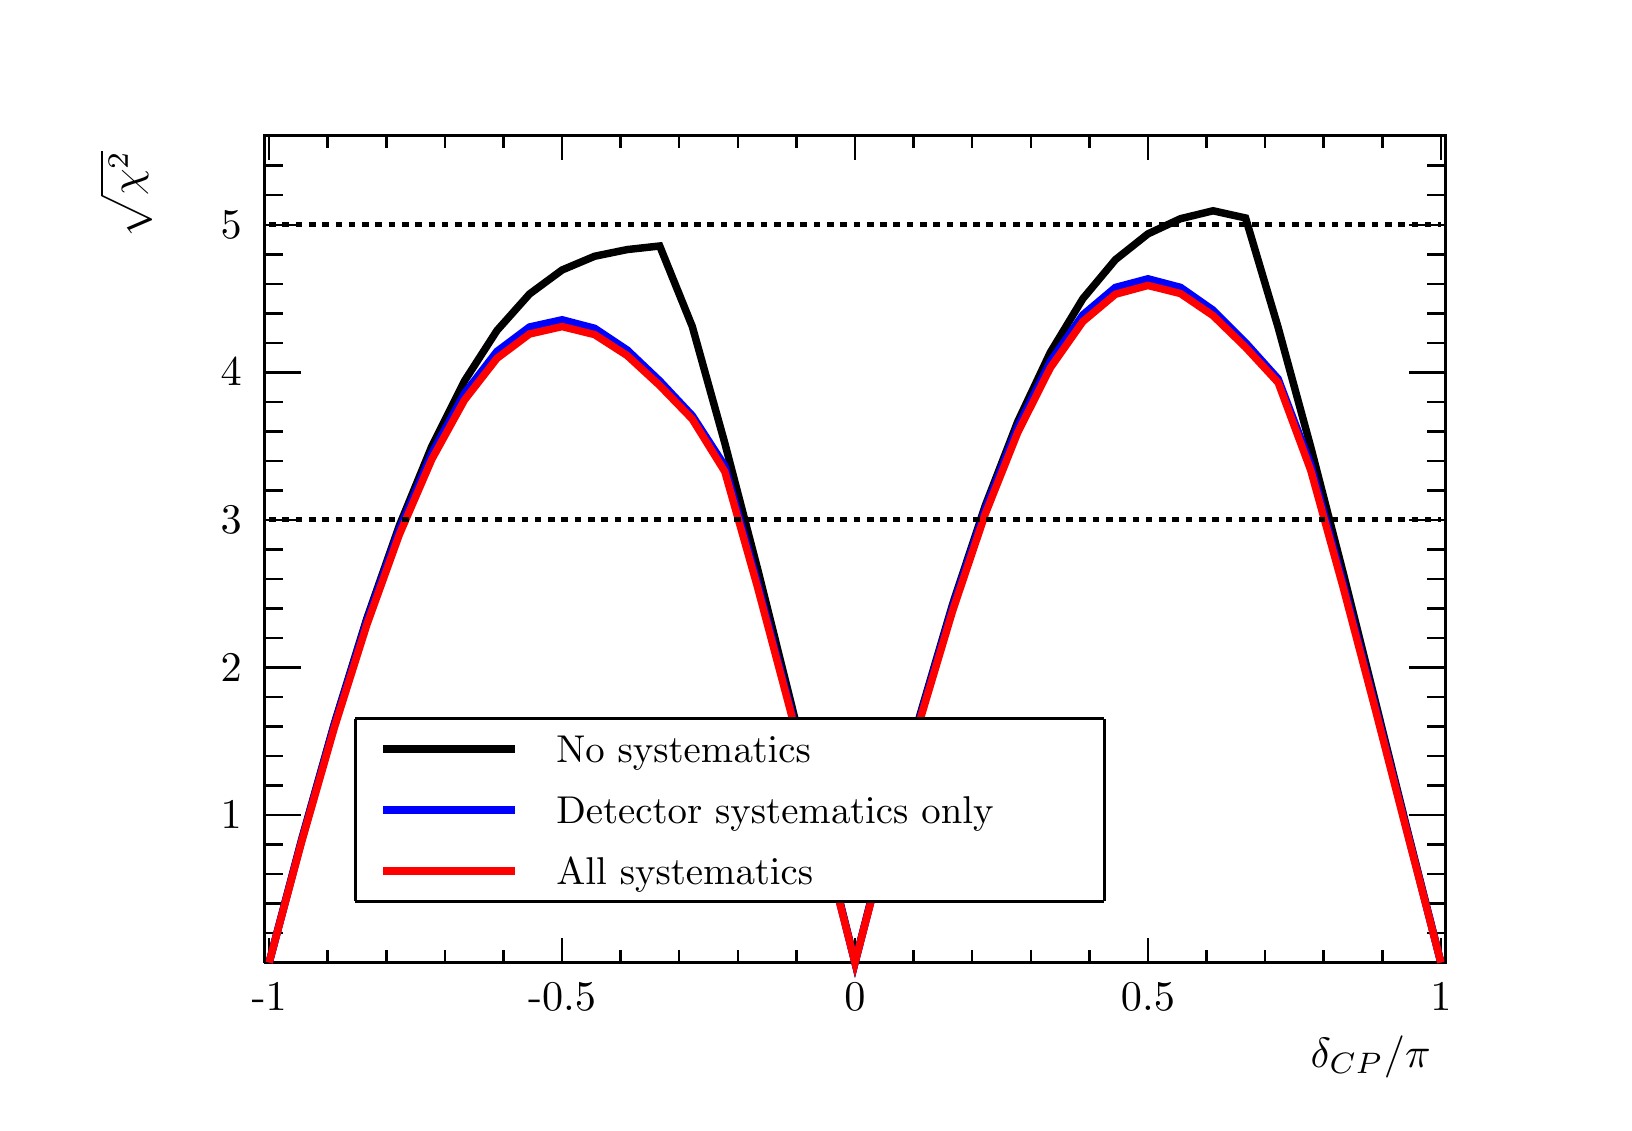
\begin{tikzpicture}
\pgfdeclareplotmark{cross} {
\pgfpathmoveto{\pgfpoint{-0.3\pgfplotmarksize}{\pgfplotmarksize}}
\pgfpathlineto{\pgfpoint{+0.3\pgfplotmarksize}{\pgfplotmarksize}}
\pgfpathlineto{\pgfpoint{+0.3\pgfplotmarksize}{0.3\pgfplotmarksize}}
\pgfpathlineto{\pgfpoint{+1\pgfplotmarksize}{0.3\pgfplotmarksize}}
\pgfpathlineto{\pgfpoint{+1\pgfplotmarksize}{-0.3\pgfplotmarksize}}
\pgfpathlineto{\pgfpoint{+0.3\pgfplotmarksize}{-0.3\pgfplotmarksize}}
\pgfpathlineto{\pgfpoint{+0.3\pgfplotmarksize}{-1.\pgfplotmarksize}}
\pgfpathlineto{\pgfpoint{-0.3\pgfplotmarksize}{-1.\pgfplotmarksize}}
\pgfpathlineto{\pgfpoint{-0.3\pgfplotmarksize}{-0.3\pgfplotmarksize}}
\pgfpathlineto{\pgfpoint{-1.\pgfplotmarksize}{-0.3\pgfplotmarksize}}
\pgfpathlineto{\pgfpoint{-1.\pgfplotmarksize}{0.3\pgfplotmarksize}}
\pgfpathlineto{\pgfpoint{-0.3\pgfplotmarksize}{0.3\pgfplotmarksize}}
\pgfpathclose
\pgfusepathqstroke
}
\pgfdeclareplotmark{cross*} {
\pgfpathmoveto{\pgfpoint{-0.3\pgfplotmarksize}{\pgfplotmarksize}}
\pgfpathlineto{\pgfpoint{+0.3\pgfplotmarksize}{\pgfplotmarksize}}
\pgfpathlineto{\pgfpoint{+0.3\pgfplotmarksize}{0.3\pgfplotmarksize}}
\pgfpathlineto{\pgfpoint{+1\pgfplotmarksize}{0.3\pgfplotmarksize}}
\pgfpathlineto{\pgfpoint{+1\pgfplotmarksize}{-0.3\pgfplotmarksize}}
\pgfpathlineto{\pgfpoint{+0.3\pgfplotmarksize}{-0.3\pgfplotmarksize}}
\pgfpathlineto{\pgfpoint{+0.3\pgfplotmarksize}{-1.\pgfplotmarksize}}
\pgfpathlineto{\pgfpoint{-0.3\pgfplotmarksize}{-1.\pgfplotmarksize}}
\pgfpathlineto{\pgfpoint{-0.3\pgfplotmarksize}{-0.3\pgfplotmarksize}}
\pgfpathlineto{\pgfpoint{-1.\pgfplotmarksize}{-0.3\pgfplotmarksize}}
\pgfpathlineto{\pgfpoint{-1.\pgfplotmarksize}{0.3\pgfplotmarksize}}
\pgfpathlineto{\pgfpoint{-0.3\pgfplotmarksize}{0.3\pgfplotmarksize}}
\pgfpathclose
\pgfusepathqfillstroke
}
\pgfdeclareplotmark{newstar} {
\pgfpathmoveto{\pgfqpoint{0pt}{\pgfplotmarksize}}
\pgfpathlineto{\pgfqpointpolar{44}{0.5\pgfplotmarksize}}
\pgfpathlineto{\pgfqpointpolar{18}{\pgfplotmarksize}}
\pgfpathlineto{\pgfqpointpolar{-20}{0.5\pgfplotmarksize}}
\pgfpathlineto{\pgfqpointpolar{-54}{\pgfplotmarksize}}
\pgfpathlineto{\pgfqpointpolar{-90}{0.5\pgfplotmarksize}}
\pgfpathlineto{\pgfqpointpolar{234}{\pgfplotmarksize}}
\pgfpathlineto{\pgfqpointpolar{198}{0.5\pgfplotmarksize}}
\pgfpathlineto{\pgfqpointpolar{162}{\pgfplotmarksize}}
\pgfpathlineto{\pgfqpointpolar{134}{0.5\pgfplotmarksize}}
\pgfpathclose
\pgfusepathqstroke
}
\pgfdeclareplotmark{newstar*} {
\pgfpathmoveto{\pgfqpoint{0pt}{\pgfplotmarksize}}
\pgfpathlineto{\pgfqpointpolar{44}{0.5\pgfplotmarksize}}
\pgfpathlineto{\pgfqpointpolar{18}{\pgfplotmarksize}}
\pgfpathlineto{\pgfqpointpolar{-20}{0.5\pgfplotmarksize}}
\pgfpathlineto{\pgfqpointpolar{-54}{\pgfplotmarksize}}
\pgfpathlineto{\pgfqpointpolar{-90}{0.5\pgfplotmarksize}}
\pgfpathlineto{\pgfqpointpolar{234}{\pgfplotmarksize}}
\pgfpathlineto{\pgfqpointpolar{198}{0.5\pgfplotmarksize}}
\pgfpathlineto{\pgfqpointpolar{162}{\pgfplotmarksize}}
\pgfpathlineto{\pgfqpointpolar{134}{0.5\pgfplotmarksize}}
\pgfpathclose
\pgfusepathqfillstroke
}
\definecolor{c}{rgb}{1,1,1};
\draw [color=c, fill=c] (0,0) rectangle (20,13.639);
\draw [color=c, fill=c] (3,1.77307) rectangle (18,12.2751);
\definecolor{c}{rgb}{0,0,0};
\draw [c,line width=0.9] (3,1.77307) -- (3,12.2751) -- (18,12.2751) -- (18,1.77307) -- (3,1.77307);
\definecolor{c}{rgb}{1,1,1};
\draw [color=c, fill=c] (3,1.77307) rectangle (18,12.2751);
\definecolor{c}{rgb}{0,0,0};
\draw [c,line width=0.9] (3,1.77307) -- (3,12.2751) -- (18,12.2751) -- (18,1.77307) -- (3,1.77307);
\draw [c,line width=0.9] (3,1.77307) -- (18,1.77307);
\draw [c,line width=0.9] (3.05952,2.07994) -- (3.05952,1.77307);
\draw [c,line width=0.9] (3.80357,1.9265) -- (3.80357,1.77307);
\draw [c,line width=0.9] (4.54762,1.9265) -- (4.54762,1.77307);
\draw [c,line width=0.9] (5.29167,1.9265) -- (5.29167,1.77307);
\draw [c,line width=0.9] (6.03571,1.9265) -- (6.03571,1.77307);
\draw [c,line width=0.9] (6.77976,2.07994) -- (6.77976,1.77307);
\draw [c,line width=0.9] (7.52381,1.9265) -- (7.52381,1.77307);
\draw [c,line width=0.9] (8.26786,1.9265) -- (8.26786,1.77307);
\draw [c,line width=0.9] (9.0119,1.9265) -- (9.0119,1.77307);
\draw [c,line width=0.9] (9.75595,1.9265) -- (9.75595,1.77307);
\draw [c,line width=0.9] (10.5,2.07994) -- (10.5,1.77307);
\draw [c,line width=0.9] (11.244,1.9265) -- (11.244,1.77307);
\draw [c,line width=0.9] (11.9881,1.9265) -- (11.9881,1.77307);
\draw [c,line width=0.9] (12.7321,1.9265) -- (12.7321,1.77307);
\draw [c,line width=0.9] (13.4762,1.9265) -- (13.4762,1.77307);
\draw [c,line width=0.9] (14.2202,2.07994) -- (14.2202,1.77307);
\draw [c,line width=0.9] (14.9643,1.9265) -- (14.9643,1.77307);
\draw [c,line width=0.9] (15.7083,1.9265) -- (15.7083,1.77307);
\draw [c,line width=0.9] (16.4524,1.9265) -- (16.4524,1.77307);
\draw [c,line width=0.9] (17.1964,1.9265) -- (17.1964,1.77307);
\draw [c,line width=0.9] (17.9405,2.07994) -- (17.9405,1.77307);
\draw [c,line width=0.9] (3.05952,2.07994) -- (3.05952,1.77307);
\draw [c,line width=0.9] (17.9405,2.07994) -- (17.9405,1.77307);
\draw [anchor=base] (3.05952,1.15931) node[scale=1.52731, color=c, rotate=0]{-1};
\draw [anchor=base] (6.77976,1.15931) node[scale=1.52731, color=c, rotate=0]{-0.5};
\draw [anchor=base] (10.5,1.15931) node[scale=1.52731, color=c, rotate=0]{0};
\draw [anchor=base] (14.2202,1.15931) node[scale=1.52731, color=c, rotate=0]{0.5};
\draw [anchor=base] (17.9405,1.15931) node[scale=1.52731, color=c, rotate=0]{1};
\draw [anchor= east] (18,0.572837) node[scale=1.52731, color=c, rotate=0]{$\delta_{CP} / \pi$};
\draw [c,line width=0.9] (3,12.2751) -- (18,12.2751);
\draw [c,line width=0.9] (3.05952,11.9682) -- (3.05952,12.2751);
\draw [c,line width=0.9] (3.80357,12.1216) -- (3.80357,12.2751);
\draw [c,line width=0.9] (4.54762,12.1216) -- (4.54762,12.2751);
\draw [c,line width=0.9] (5.29167,12.1216) -- (5.29167,12.2751);
\draw [c,line width=0.9] (6.03571,12.1216) -- (6.03571,12.2751);
\draw [c,line width=0.9] (6.77976,11.9682) -- (6.77976,12.2751);
\draw [c,line width=0.9] (7.52381,12.1216) -- (7.52381,12.2751);
\draw [c,line width=0.9] (8.26786,12.1216) -- (8.26786,12.2751);
\draw [c,line width=0.9] (9.0119,12.1216) -- (9.0119,12.2751);
\draw [c,line width=0.9] (9.75595,12.1216) -- (9.75595,12.2751);
\draw [c,line width=0.9] (10.5,11.9682) -- (10.5,12.2751);
\draw [c,line width=0.9] (11.244,12.1216) -- (11.244,12.2751);
\draw [c,line width=0.9] (11.9881,12.1216) -- (11.9881,12.2751);
\draw [c,line width=0.9] (12.7321,12.1216) -- (12.7321,12.2751);
\draw [c,line width=0.9] (13.4762,12.1216) -- (13.4762,12.2751);
\draw [c,line width=0.9] (14.2202,11.9682) -- (14.2202,12.2751);
\draw [c,line width=0.9] (14.9643,12.1216) -- (14.9643,12.2751);
\draw [c,line width=0.9] (15.7083,12.1216) -- (15.7083,12.2751);
\draw [c,line width=0.9] (16.4524,12.1216) -- (16.4524,12.2751);
\draw [c,line width=0.9] (17.1964,12.1216) -- (17.1964,12.2751);
\draw [c,line width=0.9] (17.9405,11.9682) -- (17.9405,12.2751);
\draw [c,line width=0.9] (3.05952,11.9682) -- (3.05952,12.2751);
\draw [c,line width=0.9] (17.9405,11.9682) -- (17.9405,12.2751);
\draw [c,line width=0.9] (3,1.77307) -- (3,12.2751);
\draw [c,line width=0.9] (3.462,3.64567) -- (3,3.64567);
\draw [c,line width=0.9] (3.231,4.02052) -- (3,4.02052);
\draw [c,line width=0.9] (3.231,4.39538) -- (3,4.39538);
\draw [c,line width=0.9] (3.231,4.77024) -- (3,4.77024);
\draw [c,line width=0.9] (3.231,5.14509) -- (3,5.14509);
\draw [c,line width=0.9] (3.462,5.51995) -- (3,5.51995);
\draw [c,line width=0.9] (3.231,5.89481) -- (3,5.89481);
\draw [c,line width=0.9] (3.231,6.26967) -- (3,6.26967);
\draw [c,line width=0.9] (3.231,6.64452) -- (3,6.64452);
\draw [c,line width=0.9] (3.231,7.01938) -- (3,7.01938);
\draw [c,line width=0.9] (3.462,7.39424) -- (3,7.39424);
\draw [c,line width=0.9] (3.231,7.76909) -- (3,7.76909);
\draw [c,line width=0.9] (3.231,8.14395) -- (3,8.14395);
\draw [c,line width=0.9] (3.231,8.51881) -- (3,8.51881);
\draw [c,line width=0.9] (3.231,8.89367) -- (3,8.89367);
\draw [c,line width=0.9] (3.462,9.26852) -- (3,9.26852);
\draw [c,line width=0.9] (3.231,9.64338) -- (3,9.64338);
\draw [c,line width=0.9] (3.231,10.0182) -- (3,10.0182);
\draw [c,line width=0.9] (3.231,10.3931) -- (3,10.3931);
\draw [c,line width=0.9] (3.231,10.768) -- (3,10.768);
\draw [c,line width=0.9] (3.462,11.1428) -- (3,11.1428);
\draw [c,line width=0.9] (3.462,3.64567) -- (3,3.64567);
\draw [c,line width=0.9] (3.231,3.27081) -- (3,3.27081);
\draw [c,line width=0.9] (3.231,2.89595) -- (3,2.89595);
\draw [c,line width=0.9] (3.231,2.52109) -- (3,2.52109);
\draw [c,line width=0.9] (3.231,2.14624) -- (3,2.14624);
\draw [c,line width=0.9] (3.462,11.1428) -- (3,11.1428);
\draw [c,line width=0.9] (3.231,11.5177) -- (3,11.5177);
\draw [c,line width=0.9] (3.231,11.8925) -- (3,11.8925);
\draw [c,line width=0.9] (3.231,12.2674) -- (3,12.2674);
\draw [anchor= east] (2.9,3.64567) node[scale=1.52731, color=c, rotate=0]{1};
\draw [anchor= east] (2.9,5.51995) node[scale=1.52731, color=c, rotate=0]{2};
\draw [anchor= east] (2.9,7.39424) node[scale=1.52731, color=c, rotate=0]{3};
\draw [anchor= east] (2.9,9.26852) node[scale=1.52731, color=c, rotate=0]{4};
\draw [anchor= east] (2.9,11.1428) node[scale=1.52731, color=c, rotate=0]{5};
\draw [anchor= east] (1.24,12.2751) node[scale=1.52731, color=c, rotate=90]{$\sqrt{ \chi^{2} }$};
\draw [c,line width=0.9] (18,1.77307) -- (18,12.2751);
\draw [c,line width=0.9] (17.538,3.64567) -- (18,3.64567);
\draw [c,line width=0.9] (17.769,4.02052) -- (18,4.02052);
\draw [c,line width=0.9] (17.769,4.39538) -- (18,4.39538);
\draw [c,line width=0.9] (17.769,4.77024) -- (18,4.77024);
\draw [c,line width=0.9] (17.769,5.14509) -- (18,5.14509);
\draw [c,line width=0.9] (17.538,5.51995) -- (18,5.51995);
\draw [c,line width=0.9] (17.769,5.89481) -- (18,5.89481);
\draw [c,line width=0.9] (17.769,6.26967) -- (18,6.26967);
\draw [c,line width=0.9] (17.769,6.64452) -- (18,6.64452);
\draw [c,line width=0.9] (17.769,7.01938) -- (18,7.01938);
\draw [c,line width=0.9] (17.538,7.39424) -- (18,7.39424);
\draw [c,line width=0.9] (17.769,7.76909) -- (18,7.76909);
\draw [c,line width=0.9] (17.769,8.14395) -- (18,8.14395);
\draw [c,line width=0.9] (17.769,8.51881) -- (18,8.51881);
\draw [c,line width=0.9] (17.769,8.89367) -- (18,8.89367);
\draw [c,line width=0.9] (17.538,9.26852) -- (18,9.26852);
\draw [c,line width=0.9] (17.769,9.64338) -- (18,9.64338);
\draw [c,line width=0.9] (17.769,10.0182) -- (18,10.0182);
\draw [c,line width=0.9] (17.769,10.3931) -- (18,10.3931);
\draw [c,line width=0.9] (17.769,10.768) -- (18,10.768);
\draw [c,line width=0.9] (17.538,11.1428) -- (18,11.1428);
\draw [c,line width=0.9] (17.538,3.64567) -- (18,3.64567);
\draw [c,line width=0.9] (17.769,3.27081) -- (18,3.27081);
\draw [c,line width=0.9] (17.769,2.89595) -- (18,2.89595);
\draw [c,line width=0.9] (17.769,2.52109) -- (18,2.52109);
\draw [c,line width=0.9] (17.769,2.14624) -- (18,2.14624);
\draw [c,line width=0.9] (17.538,11.1428) -- (18,11.1428);
\draw [c,line width=0.9] (17.769,11.5177) -- (18,11.5177);
\draw [c,line width=0.9] (17.769,11.8925) -- (18,11.8925);
\draw [c,line width=0.9] (17.769,12.2674) -- (18,12.2674);
\draw [c,line width=2.7] (3.05952,1.77307) -- (3.47288,3.33785) -- (3.88624,4.80397) -- (4.2996,6.1401) -- (4.71296,7.32189) -- (5.12632,8.33136) -- (5.53968,9.15795) -- (5.95304,9.79956) -- (6.3664,10.2637) -- (6.77976,10.5684) -- (7.19312,10.7429)
 -- (7.60648,10.8278) -- (8.01984,10.8733) -- (8.4332,9.85149) -- (8.84656,8.37) -- (9.25992,6.78334) -- (9.67328,5.12821) -- (10.0866,3.44506) -- (10.5,1.77307) -- (10.9134,3.39288) -- (11.3267,4.9214) -- (11.7401,6.32506) -- (12.1534,7.57311) --
 (12.5668,8.64304) -- (12.9802,9.5211) -- (13.3935,10.2038) -- (13.8069,10.6991) -- (14.2202,11.0271) -- (14.6336,11.2198) -- (15.047,11.3204) -- (15.4603,11.2289) -- (15.8737,9.83928) -- (16.287,8.32379) -- (16.7004,6.71988) -- (17.1138,5.06682) --
 (17.5271,3.40434) -- (17.9405,1.77307);
\definecolor{c}{rgb}{0,0,1};
\draw [c,line width=2.7] (3.05952,1.77307) -- (3.47288,3.32667) -- (3.88624,4.7871) -- (4.2996,6.11229) -- (4.71296,7.27285) -- (5.12632,8.24169) -- (5.53968,8.99948) -- (5.95304,9.53465) -- (6.3664,9.84443) -- (6.77976,9.93602) -- (7.19312,9.82806)
 -- (7.60648,9.55298) -- (8.01984,9.15979) -- (8.4332,8.71931) -- (8.84656,8.08045) -- (9.25992,6.60367) -- (9.67328,5.03153) -- (10.0866,3.40685) -- (10.5,1.77307) -- (10.9134,3.37158) -- (11.3267,4.89142) -- (11.7401,6.29078) -- (12.1534,7.53012)
 -- (12.5668,8.57744) -- (12.9802,9.40606) -- (13.3935,9.99829) -- (13.8069,10.3467) -- (14.2202,10.4564) -- (14.6336,10.3479) -- (15.047,10.0589) -- (15.4603,9.64583) -- (15.8737,9.18555) -- (16.287,8.09798) -- (16.7004,6.58937) -- (17.1138,5.00291)
 -- (17.5271,3.38226) -- (17.9405,1.77307);
\definecolor{c}{rgb}{1,0,0};
\draw [c,line width=2.7] (3.05952,1.77307) -- (3.47288,3.30852) -- (3.88624,4.75063) -- (4.2996,6.06105) -- (4.71296,7.20812) -- (5.12632,8.16611) -- (5.53968,8.91607) -- (5.95304,9.44675) -- (6.3664,9.75556) -- (6.77976,9.84976) -- (7.19312,9.7479)
 -- (7.60648,9.48214) -- (8.01984,9.10131) -- (8.4332,8.67462) -- (8.84656,8.00828) -- (9.25992,6.54804) -- (9.67328,4.99419) -- (10.0866,3.38759) -- (10.5,1.77307) -- (10.9134,3.35307) -- (11.3267,4.85678) -- (11.7401,6.24109) -- (12.1534,7.46813)
 -- (12.5668,8.50501) -- (12.9802,9.32593) -- (13.3935,9.91346) -- (13.8069,10.2604) -- (14.2202,10.3721) -- (14.6336,10.2691) -- (15.047,9.98875) -- (15.4603,9.58682) -- (15.8737,9.13908) -- (16.287,8.0275) -- (16.7004,6.53519) -- (17.1138,4.96565)
 -- (17.5271,3.36292) -- (17.9405,1.77307);
\definecolor{c}{rgb}{0,0,0};
\draw [c,dash pattern=on 2.40pt off 2.40pt ,line width=1.8] (3.05952,7.39424) -- (17.9405,7.39424);
\draw [c,dash pattern=on 2.40pt off 2.40pt ,line width=1.8] (3.05952,11.1428) -- (17.9405,11.1428);
\definecolor{c}{rgb}{1,1,1};
\draw [color=c, fill=c] (4.15473,2.55014) rectangle (13.6676,4.87106);
\definecolor{c}{rgb}{0,0,0};
\draw [c,line width=0.9] (4.15473,2.55014) -- (13.6676,2.55014);
\draw [c,line width=0.9] (13.6676,2.55014) -- (13.6676,4.87106);
\draw [c,line width=0.9] (13.6676,4.87106) -- (4.15473,4.87106);
\draw [c,line width=0.9] (4.15473,4.87106) -- (4.15473,2.55014);
\draw [anchor=base west] (6.53295,4.31017) node[scale=1.40004, color=c, rotate=0]{No systematics};
\definecolor{c}{rgb}{1,1,1};
\draw [c, fill=c] (4.51146,4.21347) -- (6.17622,4.21347) -- (6.17622,4.75501) -- (4.51146,4.75501);
\definecolor{c}{rgb}{0,0,0};
\draw [c,line width=2.7] (4.51146,4.48424) -- (6.17622,4.48424);
\foreach \P in {(5.34384,4.48424)}{\draw[mark options={color=c,fill=c},mark size=2.402402pt, line width=0.000000pt, mark=*,mark size=1pt] plot coordinates {\P};}
\draw [anchor=base west] (6.53295,3.53653) node[scale=1.40004, color=c, rotate=0]{Detector systematics only};
\definecolor{c}{rgb}{1,1,1};
\draw [c, fill=c] (4.51146,3.43983) -- (6.17622,3.43983) -- (6.17622,3.98138) -- (4.51146,3.98138);
\definecolor{c}{rgb}{0,0,1};
\draw [c,line width=2.7] (4.51146,3.7106) -- (6.17622,3.7106);
\foreach \P in {(5.34384,3.7106)}{\draw[mark options={color=c,fill=c},mark size=2.402402pt, line width=0.000000pt, mark=*,mark size=1pt] plot coordinates {\P};}
\definecolor{c}{rgb}{0,0,0};
\draw [anchor=base west] (6.53295,2.76289) node[scale=1.40004, color=c, rotate=0]{All systematics};
\definecolor{c}{rgb}{1,1,1};
\draw [c, fill=c] (4.51146,2.66619) -- (6.17622,2.66619) -- (6.17622,3.20774) -- (4.51146,3.20774);
\definecolor{c}{rgb}{1,0,0};
\draw [c,line width=2.7] (4.51146,2.93696) -- (6.17622,2.93696);
\foreach \P in {(5.34384,2.93696)}{\draw[mark options={color=c,fill=c},mark size=2.402402pt, line width=0.000000pt, mark=*,mark size=1pt] plot coordinates {\P};}
\end{tikzpicture}

		\end{adjustbox}
	\end{minipage}
	\hfill
	\begin{minipage}[t]{.5\linewidth}
		\begin{adjustbox}{max totalsize=\linewidth, center}
			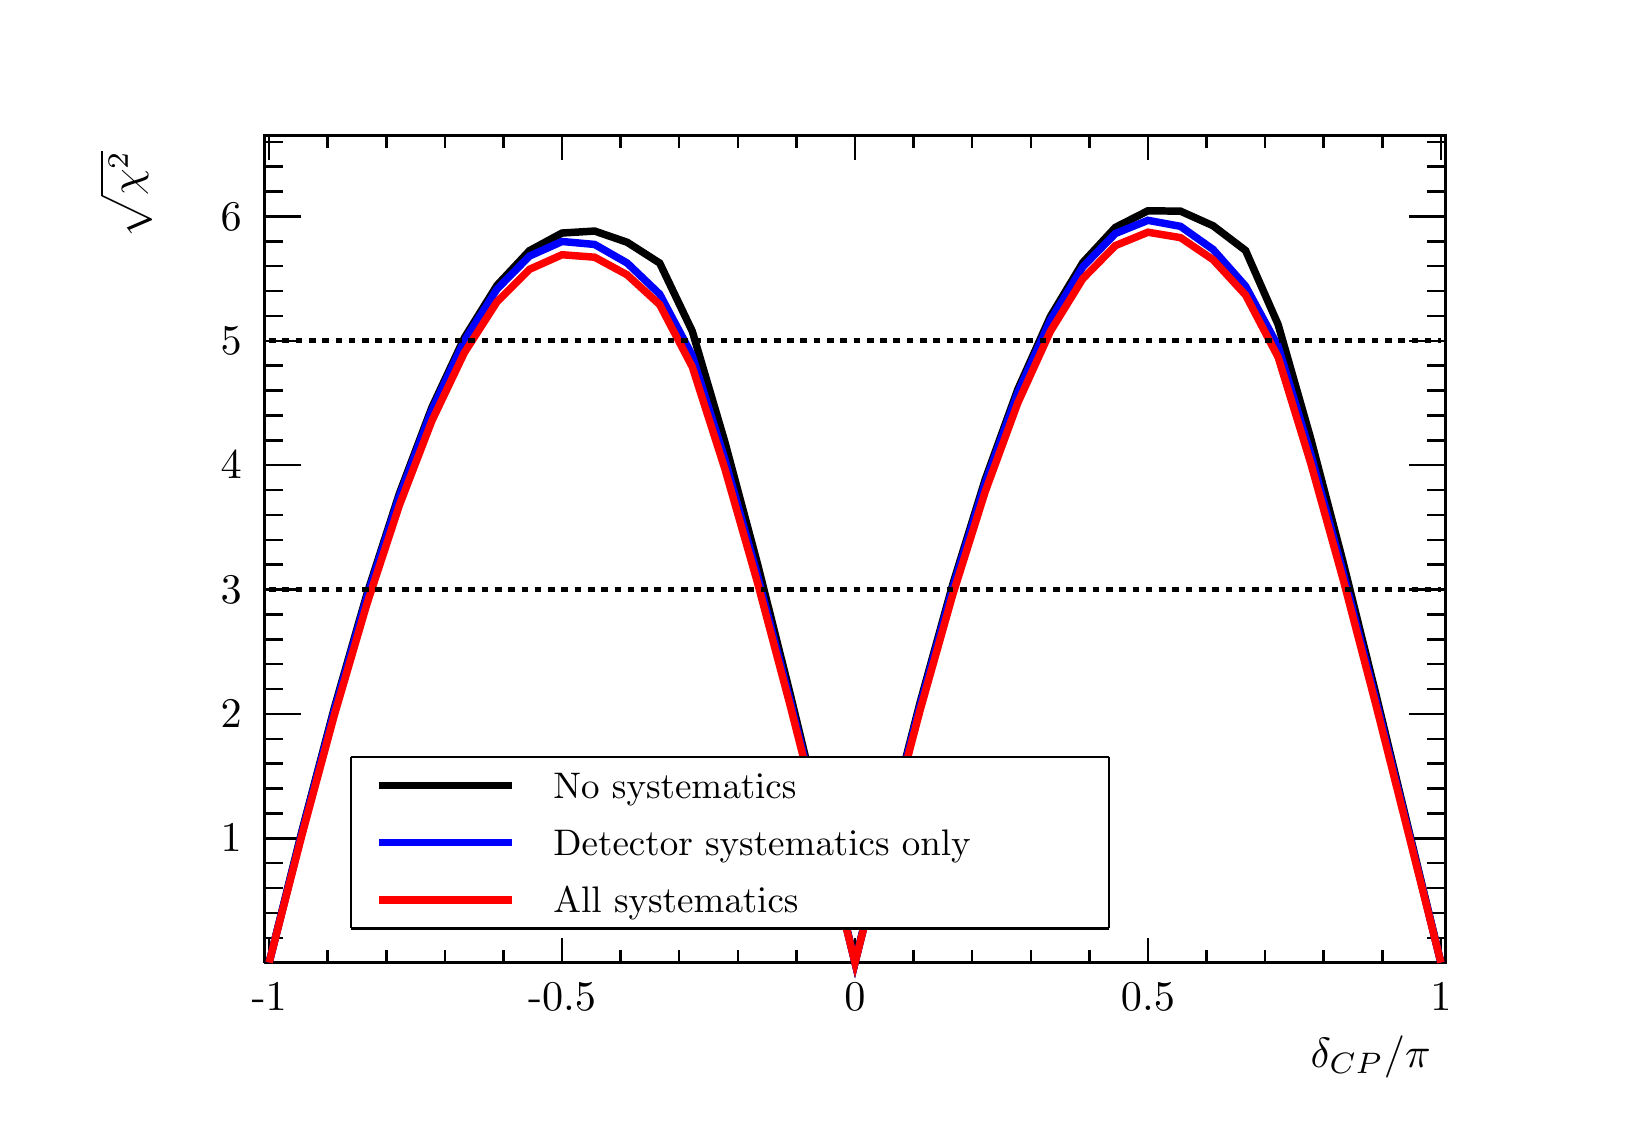
\begin{tikzpicture}
\pgfdeclareplotmark{cross} {
\pgfpathmoveto{\pgfpoint{-0.3\pgfplotmarksize}{\pgfplotmarksize}}
\pgfpathlineto{\pgfpoint{+0.3\pgfplotmarksize}{\pgfplotmarksize}}
\pgfpathlineto{\pgfpoint{+0.3\pgfplotmarksize}{0.3\pgfplotmarksize}}
\pgfpathlineto{\pgfpoint{+1\pgfplotmarksize}{0.3\pgfplotmarksize}}
\pgfpathlineto{\pgfpoint{+1\pgfplotmarksize}{-0.3\pgfplotmarksize}}
\pgfpathlineto{\pgfpoint{+0.3\pgfplotmarksize}{-0.3\pgfplotmarksize}}
\pgfpathlineto{\pgfpoint{+0.3\pgfplotmarksize}{-1.\pgfplotmarksize}}
\pgfpathlineto{\pgfpoint{-0.3\pgfplotmarksize}{-1.\pgfplotmarksize}}
\pgfpathlineto{\pgfpoint{-0.3\pgfplotmarksize}{-0.3\pgfplotmarksize}}
\pgfpathlineto{\pgfpoint{-1.\pgfplotmarksize}{-0.3\pgfplotmarksize}}
\pgfpathlineto{\pgfpoint{-1.\pgfplotmarksize}{0.3\pgfplotmarksize}}
\pgfpathlineto{\pgfpoint{-0.3\pgfplotmarksize}{0.3\pgfplotmarksize}}
\pgfpathclose
\pgfusepathqstroke
}
\pgfdeclareplotmark{cross*} {
\pgfpathmoveto{\pgfpoint{-0.3\pgfplotmarksize}{\pgfplotmarksize}}
\pgfpathlineto{\pgfpoint{+0.3\pgfplotmarksize}{\pgfplotmarksize}}
\pgfpathlineto{\pgfpoint{+0.3\pgfplotmarksize}{0.3\pgfplotmarksize}}
\pgfpathlineto{\pgfpoint{+1\pgfplotmarksize}{0.3\pgfplotmarksize}}
\pgfpathlineto{\pgfpoint{+1\pgfplotmarksize}{-0.3\pgfplotmarksize}}
\pgfpathlineto{\pgfpoint{+0.3\pgfplotmarksize}{-0.3\pgfplotmarksize}}
\pgfpathlineto{\pgfpoint{+0.3\pgfplotmarksize}{-1.\pgfplotmarksize}}
\pgfpathlineto{\pgfpoint{-0.3\pgfplotmarksize}{-1.\pgfplotmarksize}}
\pgfpathlineto{\pgfpoint{-0.3\pgfplotmarksize}{-0.3\pgfplotmarksize}}
\pgfpathlineto{\pgfpoint{-1.\pgfplotmarksize}{-0.3\pgfplotmarksize}}
\pgfpathlineto{\pgfpoint{-1.\pgfplotmarksize}{0.3\pgfplotmarksize}}
\pgfpathlineto{\pgfpoint{-0.3\pgfplotmarksize}{0.3\pgfplotmarksize}}
\pgfpathclose
\pgfusepathqfillstroke
}
\pgfdeclareplotmark{newstar} {
\pgfpathmoveto{\pgfqpoint{0pt}{\pgfplotmarksize}}
\pgfpathlineto{\pgfqpointpolar{44}{0.5\pgfplotmarksize}}
\pgfpathlineto{\pgfqpointpolar{18}{\pgfplotmarksize}}
\pgfpathlineto{\pgfqpointpolar{-20}{0.5\pgfplotmarksize}}
\pgfpathlineto{\pgfqpointpolar{-54}{\pgfplotmarksize}}
\pgfpathlineto{\pgfqpointpolar{-90}{0.5\pgfplotmarksize}}
\pgfpathlineto{\pgfqpointpolar{234}{\pgfplotmarksize}}
\pgfpathlineto{\pgfqpointpolar{198}{0.5\pgfplotmarksize}}
\pgfpathlineto{\pgfqpointpolar{162}{\pgfplotmarksize}}
\pgfpathlineto{\pgfqpointpolar{134}{0.5\pgfplotmarksize}}
\pgfpathclose
\pgfusepathqstroke
}
\pgfdeclareplotmark{newstar*} {
\pgfpathmoveto{\pgfqpoint{0pt}{\pgfplotmarksize}}
\pgfpathlineto{\pgfqpointpolar{44}{0.5\pgfplotmarksize}}
\pgfpathlineto{\pgfqpointpolar{18}{\pgfplotmarksize}}
\pgfpathlineto{\pgfqpointpolar{-20}{0.5\pgfplotmarksize}}
\pgfpathlineto{\pgfqpointpolar{-54}{\pgfplotmarksize}}
\pgfpathlineto{\pgfqpointpolar{-90}{0.5\pgfplotmarksize}}
\pgfpathlineto{\pgfqpointpolar{234}{\pgfplotmarksize}}
\pgfpathlineto{\pgfqpointpolar{198}{0.5\pgfplotmarksize}}
\pgfpathlineto{\pgfqpointpolar{162}{\pgfplotmarksize}}
\pgfpathlineto{\pgfqpointpolar{134}{0.5\pgfplotmarksize}}
\pgfpathclose
\pgfusepathqfillstroke
}
\definecolor{c}{rgb}{1,1,1};
\draw [color=c, fill=c] (0,0) rectangle (20,13.639);
\draw [color=c, fill=c] (3,1.77307) rectangle (18,12.2751);
\definecolor{c}{rgb}{0,0,0};
\draw [c,line width=0.9] (3,1.77307) -- (3,12.2751) -- (18,12.2751) -- (18,1.77307) -- (3,1.77307);
\definecolor{c}{rgb}{1,1,1};
\draw [color=c, fill=c] (3,1.77307) rectangle (18,12.2751);
\definecolor{c}{rgb}{0,0,0};
\draw [c,line width=0.9] (3,1.77307) -- (3,12.2751) -- (18,12.2751) -- (18,1.77307) -- (3,1.77307);
\draw [c,line width=0.9] (3,1.77307) -- (18,1.77307);
\draw [c,line width=0.9] (3.05952,2.07994) -- (3.05952,1.77307);
\draw [c,line width=0.9] (3.80357,1.9265) -- (3.80357,1.77307);
\draw [c,line width=0.9] (4.54762,1.9265) -- (4.54762,1.77307);
\draw [c,line width=0.9] (5.29167,1.9265) -- (5.29167,1.77307);
\draw [c,line width=0.9] (6.03571,1.9265) -- (6.03571,1.77307);
\draw [c,line width=0.9] (6.77976,2.07994) -- (6.77976,1.77307);
\draw [c,line width=0.9] (7.52381,1.9265) -- (7.52381,1.77307);
\draw [c,line width=0.9] (8.26786,1.9265) -- (8.26786,1.77307);
\draw [c,line width=0.9] (9.0119,1.9265) -- (9.0119,1.77307);
\draw [c,line width=0.9] (9.75595,1.9265) -- (9.75595,1.77307);
\draw [c,line width=0.9] (10.5,2.07994) -- (10.5,1.77307);
\draw [c,line width=0.9] (11.244,1.9265) -- (11.244,1.77307);
\draw [c,line width=0.9] (11.9881,1.9265) -- (11.9881,1.77307);
\draw [c,line width=0.9] (12.7321,1.9265) -- (12.7321,1.77307);
\draw [c,line width=0.9] (13.4762,1.9265) -- (13.4762,1.77307);
\draw [c,line width=0.9] (14.2202,2.07994) -- (14.2202,1.77307);
\draw [c,line width=0.9] (14.9643,1.9265) -- (14.9643,1.77307);
\draw [c,line width=0.9] (15.7083,1.9265) -- (15.7083,1.77307);
\draw [c,line width=0.9] (16.4524,1.9265) -- (16.4524,1.77307);
\draw [c,line width=0.9] (17.1964,1.9265) -- (17.1964,1.77307);
\draw [c,line width=0.9] (17.9405,2.07994) -- (17.9405,1.77307);
\draw [c,line width=0.9] (3.05952,2.07994) -- (3.05952,1.77307);
\draw [c,line width=0.9] (17.9405,2.07994) -- (17.9405,1.77307);
\draw [anchor=base] (3.05952,1.15931) node[scale=1.52731, color=c, rotate=0]{-1};
\draw [anchor=base] (6.77976,1.15931) node[scale=1.52731, color=c, rotate=0]{-0.5};
\draw [anchor=base] (10.5,1.15931) node[scale=1.52731, color=c, rotate=0]{0};
\draw [anchor=base] (14.2202,1.15931) node[scale=1.52731, color=c, rotate=0]{0.5};
\draw [anchor=base] (17.9405,1.15931) node[scale=1.52731, color=c, rotate=0]{1};
\draw [anchor= east] (18,0.572837) node[scale=1.52731, color=c, rotate=0]{$\delta_{CP} / \pi$};
\draw [c,line width=0.9] (3,12.2751) -- (18,12.2751);
\draw [c,line width=0.9] (3.05952,11.9682) -- (3.05952,12.2751);
\draw [c,line width=0.9] (3.80357,12.1216) -- (3.80357,12.2751);
\draw [c,line width=0.9] (4.54762,12.1216) -- (4.54762,12.2751);
\draw [c,line width=0.9] (5.29167,12.1216) -- (5.29167,12.2751);
\draw [c,line width=0.9] (6.03571,12.1216) -- (6.03571,12.2751);
\draw [c,line width=0.9] (6.77976,11.9682) -- (6.77976,12.2751);
\draw [c,line width=0.9] (7.52381,12.1216) -- (7.52381,12.2751);
\draw [c,line width=0.9] (8.26786,12.1216) -- (8.26786,12.2751);
\draw [c,line width=0.9] (9.0119,12.1216) -- (9.0119,12.2751);
\draw [c,line width=0.9] (9.75595,12.1216) -- (9.75595,12.2751);
\draw [c,line width=0.9] (10.5,11.9682) -- (10.5,12.2751);
\draw [c,line width=0.9] (11.244,12.1216) -- (11.244,12.2751);
\draw [c,line width=0.9] (11.9881,12.1216) -- (11.9881,12.2751);
\draw [c,line width=0.9] (12.7321,12.1216) -- (12.7321,12.2751);
\draw [c,line width=0.9] (13.4762,12.1216) -- (13.4762,12.2751);
\draw [c,line width=0.9] (14.2202,11.9682) -- (14.2202,12.2751);
\draw [c,line width=0.9] (14.9643,12.1216) -- (14.9643,12.2751);
\draw [c,line width=0.9] (15.7083,12.1216) -- (15.7083,12.2751);
\draw [c,line width=0.9] (16.4524,12.1216) -- (16.4524,12.2751);
\draw [c,line width=0.9] (17.1964,12.1216) -- (17.1964,12.2751);
\draw [c,line width=0.9] (17.9405,11.9682) -- (17.9405,12.2751);
\draw [c,line width=0.9] (3.05952,11.9682) -- (3.05952,12.2751);
\draw [c,line width=0.9] (17.9405,11.9682) -- (17.9405,12.2751);
\draw [c,line width=0.9] (3,1.77307) -- (3,12.2751);
\draw [c,line width=0.9] (3.462,3.35114) -- (3,3.35114);
\draw [c,line width=0.9] (3.231,3.66704) -- (3,3.66704);
\draw [c,line width=0.9] (3.231,3.98294) -- (3,3.98294);
\draw [c,line width=0.9] (3.231,4.29884) -- (3,4.29884);
\draw [c,line width=0.9] (3.231,4.61474) -- (3,4.61474);
\draw [c,line width=0.9] (3.462,4.93064) -- (3,4.93064);
\draw [c,line width=0.9] (3.231,5.24654) -- (3,5.24654);
\draw [c,line width=0.9] (3.231,5.56244) -- (3,5.56244);
\draw [c,line width=0.9] (3.231,5.87834) -- (3,5.87834);
\draw [c,line width=0.9] (3.231,6.19424) -- (3,6.19424);
\draw [c,line width=0.9] (3.462,6.51014) -- (3,6.51014);
\draw [c,line width=0.9] (3.231,6.82604) -- (3,6.82604);
\draw [c,line width=0.9] (3.231,7.14194) -- (3,7.14194);
\draw [c,line width=0.9] (3.231,7.45784) -- (3,7.45784);
\draw [c,line width=0.9] (3.231,7.77373) -- (3,7.77373);
\draw [c,line width=0.9] (3.462,8.08963) -- (3,8.08963);
\draw [c,line width=0.9] (3.231,8.40553) -- (3,8.40553);
\draw [c,line width=0.9] (3.231,8.72143) -- (3,8.72143);
\draw [c,line width=0.9] (3.231,9.03733) -- (3,9.03733);
\draw [c,line width=0.9] (3.231,9.35323) -- (3,9.35323);
\draw [c,line width=0.9] (3.462,9.66913) -- (3,9.66913);
\draw [c,line width=0.9] (3.231,9.98503) -- (3,9.98503);
\draw [c,line width=0.9] (3.231,10.3009) -- (3,10.3009);
\draw [c,line width=0.9] (3.231,10.6168) -- (3,10.6168);
\draw [c,line width=0.9] (3.231,10.9327) -- (3,10.9327);
\draw [c,line width=0.9] (3.462,11.2486) -- (3,11.2486);
\draw [c,line width=0.9] (3.462,3.35114) -- (3,3.35114);
\draw [c,line width=0.9] (3.231,3.03524) -- (3,3.03524);
\draw [c,line width=0.9] (3.231,2.71934) -- (3,2.71934);
\draw [c,line width=0.9] (3.231,2.40344) -- (3,2.40344);
\draw [c,line width=0.9] (3.231,2.08754) -- (3,2.08754);
\draw [c,line width=0.9] (3.462,11.2486) -- (3,11.2486);
\draw [c,line width=0.9] (3.231,11.5645) -- (3,11.5645);
\draw [c,line width=0.9] (3.231,11.8804) -- (3,11.8804);
\draw [c,line width=0.9] (3.231,12.1963) -- (3,12.1963);
\draw [anchor= east] (2.9,3.35114) node[scale=1.52731, color=c, rotate=0]{1};
\draw [anchor= east] (2.9,4.93064) node[scale=1.52731, color=c, rotate=0]{2};
\draw [anchor= east] (2.9,6.51014) node[scale=1.52731, color=c, rotate=0]{3};
\draw [anchor= east] (2.9,8.08963) node[scale=1.52731, color=c, rotate=0]{4};
\draw [anchor= east] (2.9,9.66913) node[scale=1.52731, color=c, rotate=0]{5};
\draw [anchor= east] (2.9,11.2486) node[scale=1.52731, color=c, rotate=0]{6};
\draw [anchor= east] (1.24,12.2751) node[scale=1.52731, color=c, rotate=90]{$\sqrt{ \chi^{2} }$};
\draw [c,line width=0.9] (18,1.77307) -- (18,12.2751);
\draw [c,line width=0.9] (17.538,3.35114) -- (18,3.35114);
\draw [c,line width=0.9] (17.769,3.66704) -- (18,3.66704);
\draw [c,line width=0.9] (17.769,3.98294) -- (18,3.98294);
\draw [c,line width=0.9] (17.769,4.29884) -- (18,4.29884);
\draw [c,line width=0.9] (17.769,4.61474) -- (18,4.61474);
\draw [c,line width=0.9] (17.538,4.93064) -- (18,4.93064);
\draw [c,line width=0.9] (17.769,5.24654) -- (18,5.24654);
\draw [c,line width=0.9] (17.769,5.56244) -- (18,5.56244);
\draw [c,line width=0.9] (17.769,5.87834) -- (18,5.87834);
\draw [c,line width=0.9] (17.769,6.19424) -- (18,6.19424);
\draw [c,line width=0.9] (17.538,6.51014) -- (18,6.51014);
\draw [c,line width=0.9] (17.769,6.82604) -- (18,6.82604);
\draw [c,line width=0.9] (17.769,7.14194) -- (18,7.14194);
\draw [c,line width=0.9] (17.769,7.45784) -- (18,7.45784);
\draw [c,line width=0.9] (17.769,7.77373) -- (18,7.77373);
\draw [c,line width=0.9] (17.538,8.08963) -- (18,8.08963);
\draw [c,line width=0.9] (17.769,8.40553) -- (18,8.40553);
\draw [c,line width=0.9] (17.769,8.72143) -- (18,8.72143);
\draw [c,line width=0.9] (17.769,9.03733) -- (18,9.03733);
\draw [c,line width=0.9] (17.769,9.35323) -- (18,9.35323);
\draw [c,line width=0.9] (17.538,9.66913) -- (18,9.66913);
\draw [c,line width=0.9] (17.769,9.98503) -- (18,9.98503);
\draw [c,line width=0.9] (17.769,10.3009) -- (18,10.3009);
\draw [c,line width=0.9] (17.769,10.6168) -- (18,10.6168);
\draw [c,line width=0.9] (17.769,10.9327) -- (18,10.9327);
\draw [c,line width=0.9] (17.538,11.2486) -- (18,11.2486);
\draw [c,line width=0.9] (17.538,3.35114) -- (18,3.35114);
\draw [c,line width=0.9] (17.769,3.03524) -- (18,3.03524);
\draw [c,line width=0.9] (17.769,2.71934) -- (18,2.71934);
\draw [c,line width=0.9] (17.769,2.40344) -- (18,2.40344);
\draw [c,line width=0.9] (17.769,2.08754) -- (18,2.08754);
\draw [c,line width=0.9] (17.538,11.2486) -- (18,11.2486);
\draw [c,line width=0.9] (17.769,11.5645) -- (18,11.5645);
\draw [c,line width=0.9] (17.769,11.8804) -- (18,11.8804);
\draw [c,line width=0.9] (17.769,12.1963) -- (18,12.1963);
\draw [c,line width=2.7] (3.05952,1.77307) -- (3.47288,3.43116) -- (3.88624,5.00182) -- (4.2996,6.4452) -- (4.71296,7.7278) -- (5.12632,8.82218) -- (5.53968,9.708) -- (5.95304,10.373) -- (6.3664,10.8141) -- (6.77976,11.038) -- (7.19312,11.063) --
 (7.60648,10.9205) -- (8.01984,10.656) -- (8.4332,9.79109) -- (8.84656,8.38708) -- (9.25992,6.84323) -- (9.67328,5.19766) -- (10.0866,3.49229) -- (10.5,1.77307) -- (10.9134,3.46183) -- (11.3267,5.07613) -- (11.7401,6.57113) -- (12.1534,7.90723) --
 (12.5668,9.05057) -- (12.9802,9.97487) -- (13.3935,10.6632) -- (13.8069,11.1096) -- (14.2202,11.3204) -- (14.6336,11.3155) -- (15.047,11.1303) -- (15.4603,10.816) -- (15.8737,9.87595) -- (16.287,8.42903) -- (16.7004,6.85164) -- (17.1138,5.18634) --
 (17.5271,3.47788) -- (17.9405,1.77307);
\definecolor{c}{rgb}{0,0,1};
\draw [c,line width=2.7] (3.05952,1.77307) -- (3.47288,3.4123) -- (3.88624,4.97155) -- (4.2996,6.41047) -- (4.71296,7.69272) -- (5.12632,8.78711) -- (5.53968,9.67057) -- (5.95304,10.3257) -- (6.3664,10.7453) -- (6.77976,10.9303) -- (7.19312,10.8929)
 -- (7.60648,10.6569) -- (8.01984,10.2613) -- (8.4332,9.48296) -- (8.84656,8.16636) -- (9.25992,6.69708) -- (9.67328,5.11322) -- (10.0866,3.45713) -- (10.5,1.77307) -- (10.9134,3.43855) -- (11.3267,5.03785) -- (11.7401,6.52715) -- (12.1534,7.86237)
 -- (12.5668,9.00653) -- (12.9802,9.92945) -- (13.3935,10.6086) -- (13.8069,11.0318) -- (14.2202,11.1991) -- (14.6336,11.1228) -- (15.047,10.8297) -- (15.4603,10.3629) -- (15.8737,9.59968) -- (16.287,8.23334) -- (16.7004,6.72366) -- (17.1138,5.11329)
 -- (17.5271,3.44816) -- (17.9405,1.77307);
\definecolor{c}{rgb}{1,0,0};
\draw [c,line width=2.7] (3.05952,1.77307) -- (3.47288,3.38027) -- (3.88624,4.91019) -- (4.2996,6.32155) -- (4.71296,7.57896) -- (5.12632,8.65266) -- (5.53968,9.51941) -- (5.95304,10.1634) -- (6.3664,10.5771) -- (6.77976,10.7622) -- (7.19312,10.7308)
 -- (7.60648,10.5067) -- (8.01984,10.128) -- (8.4332,9.33814) -- (8.84656,8.04578) -- (9.25992,6.60409) -- (9.67328,5.05001) -- (10.0866,3.42455) -- (10.5,1.77307) -- (10.9134,3.40654) -- (11.3267,4.97764) -- (11.7401,6.4403) -- (12.1534,7.75289) --
 (12.5668,8.87865) -- (12.9802,9.78756) -- (13.3935,10.458) -- (13.8069,10.8783) -- (14.2202,11.048) -- (14.6336,10.9795) -- (15.047,10.6995) -- (15.4603,10.2503) -- (15.8737,9.46081) -- (16.287,8.11693) -- (16.7004,6.63336) -- (17.1138,5.05168) --
 (17.5271,3.41607) -- (17.9405,1.77307);
\definecolor{c}{rgb}{0,0,0};
\draw [c,dash pattern=on 2.40pt off 2.40pt ,line width=1.8] (3.05952,6.51014) -- (17.9405,6.51014);
\draw [c,dash pattern=on 2.40pt off 2.40pt ,line width=1.8] (3.05952,9.66913) -- (17.9405,9.66913);
\definecolor{c}{rgb}{1,1,1};
\draw [color=c, fill=c] (4.09742,2.2063) rectangle (13.7249,4.38395);
\definecolor{c}{rgb}{0,0,0};
\draw [c,line width=0.9] (4.09742,2.2063) -- (13.7249,2.2063);
\draw [c,line width=0.9] (13.7249,2.2063) -- (13.7249,4.38395);
\draw [c,line width=0.9] (13.7249,4.38395) -- (4.09742,4.38395);
\draw [c,line width=0.9] (4.09742,4.38395) -- (4.09742,2.2063);
\draw [anchor=base west] (6.5043,3.85769) node[scale=1.3364, color=c, rotate=0]{No systematics};
\draw [c,line width=2.7] (4.45845,4.02101) -- (6.14327,4.02101);
\draw [anchor=base west] (6.5043,3.13181) node[scale=1.3364, color=c, rotate=0]{Detector systematics only};
\definecolor{c}{rgb}{1,1,1};
\draw [c, fill=c] (4.45845,3.04107) -- (6.14327,3.04107) -- (6.14327,3.54919) -- (4.45845,3.54919);
\definecolor{c}{rgb}{0,0,1};
\draw [c,line width=2.7] (4.45845,3.29513) -- (6.14327,3.29513);
\foreach \P in {(5.30086,3.29513)}{\draw[mark options={color=c,fill=c},mark size=2.402402pt, line width=0.000000pt, mark=*,mark size=1pt] plot coordinates {\P};}
\definecolor{c}{rgb}{0,0,0};
\draw [anchor=base west] (6.5043,2.40592) node[scale=1.3364, color=c, rotate=0]{All systematics};
\definecolor{c}{rgb}{1,0,0};
\draw [c,line width=2.7] (4.45845,2.56925) -- (6.14327,2.56925);
\end{tikzpicture}

		\end{adjustbox}
	\end{minipage}
	\caption[DUNE sensitivities to CP-violation in the lepton sector as a function of true \dcp.]{DUNE sensitivities to CP-violation in the lepton sector as a function of true \dcp for 7 years of staged running. The black line shows the statistics-only case. The blue line shows the case where only the detector systematics are used. The red line shows the case where all systematics are used. Left: True normal neutrino mass hierarchy. Right: True inverted mass hierarchy.}
	\label{fig:cpvSens}
\end{figure}

Looking at \citefig{fig:cpvSens}, one can see that DUNE's sensitivity is slightly better in the case that the true neutrino mass hierarchy is inverted rather than normal.
In the case of the inverted hierarchy, after 7 years of running DUNE will have the potential to discover CPV if the true value of \dcp is near $-\pi/2$ or $\pi/2$ even with all systematics.
However, if the mass hierarchy is normal then DUNE's CPV discovery potential is lower. 
Under this 7 year running plan, DUNE will not reach the crucial $5\sigma$ discovery level when systematics are included. 
However, DUNE will still exceed the $3\sigma$ threshold for many values of \dcp with the full suite of systematics.

One interesting point that is observable in \citefig{fig:cpvSens} is that that most of the decrease in sensitivity from the statistics-only case occurs when only including the detector systematics.
Although there is a decrease from the blue to the red line upon the inclusion of the flux and cross-section systematics, it is much less substantial than the drop in sensitivity upon the inclusion of just the detector systematics.
It can therefore be assumed that in order for DUNE to reach its full potential, it will be very important to control the detector systematics.
